%---------------------------------------------------------------------
\subsection{Supplementary Results: Phylogenies and priors}
%---------------------------------------------------------------------
\subsubsection{\textit{Full} tree}
%---------------------------------------------------------------------

\begin{figure}[H]
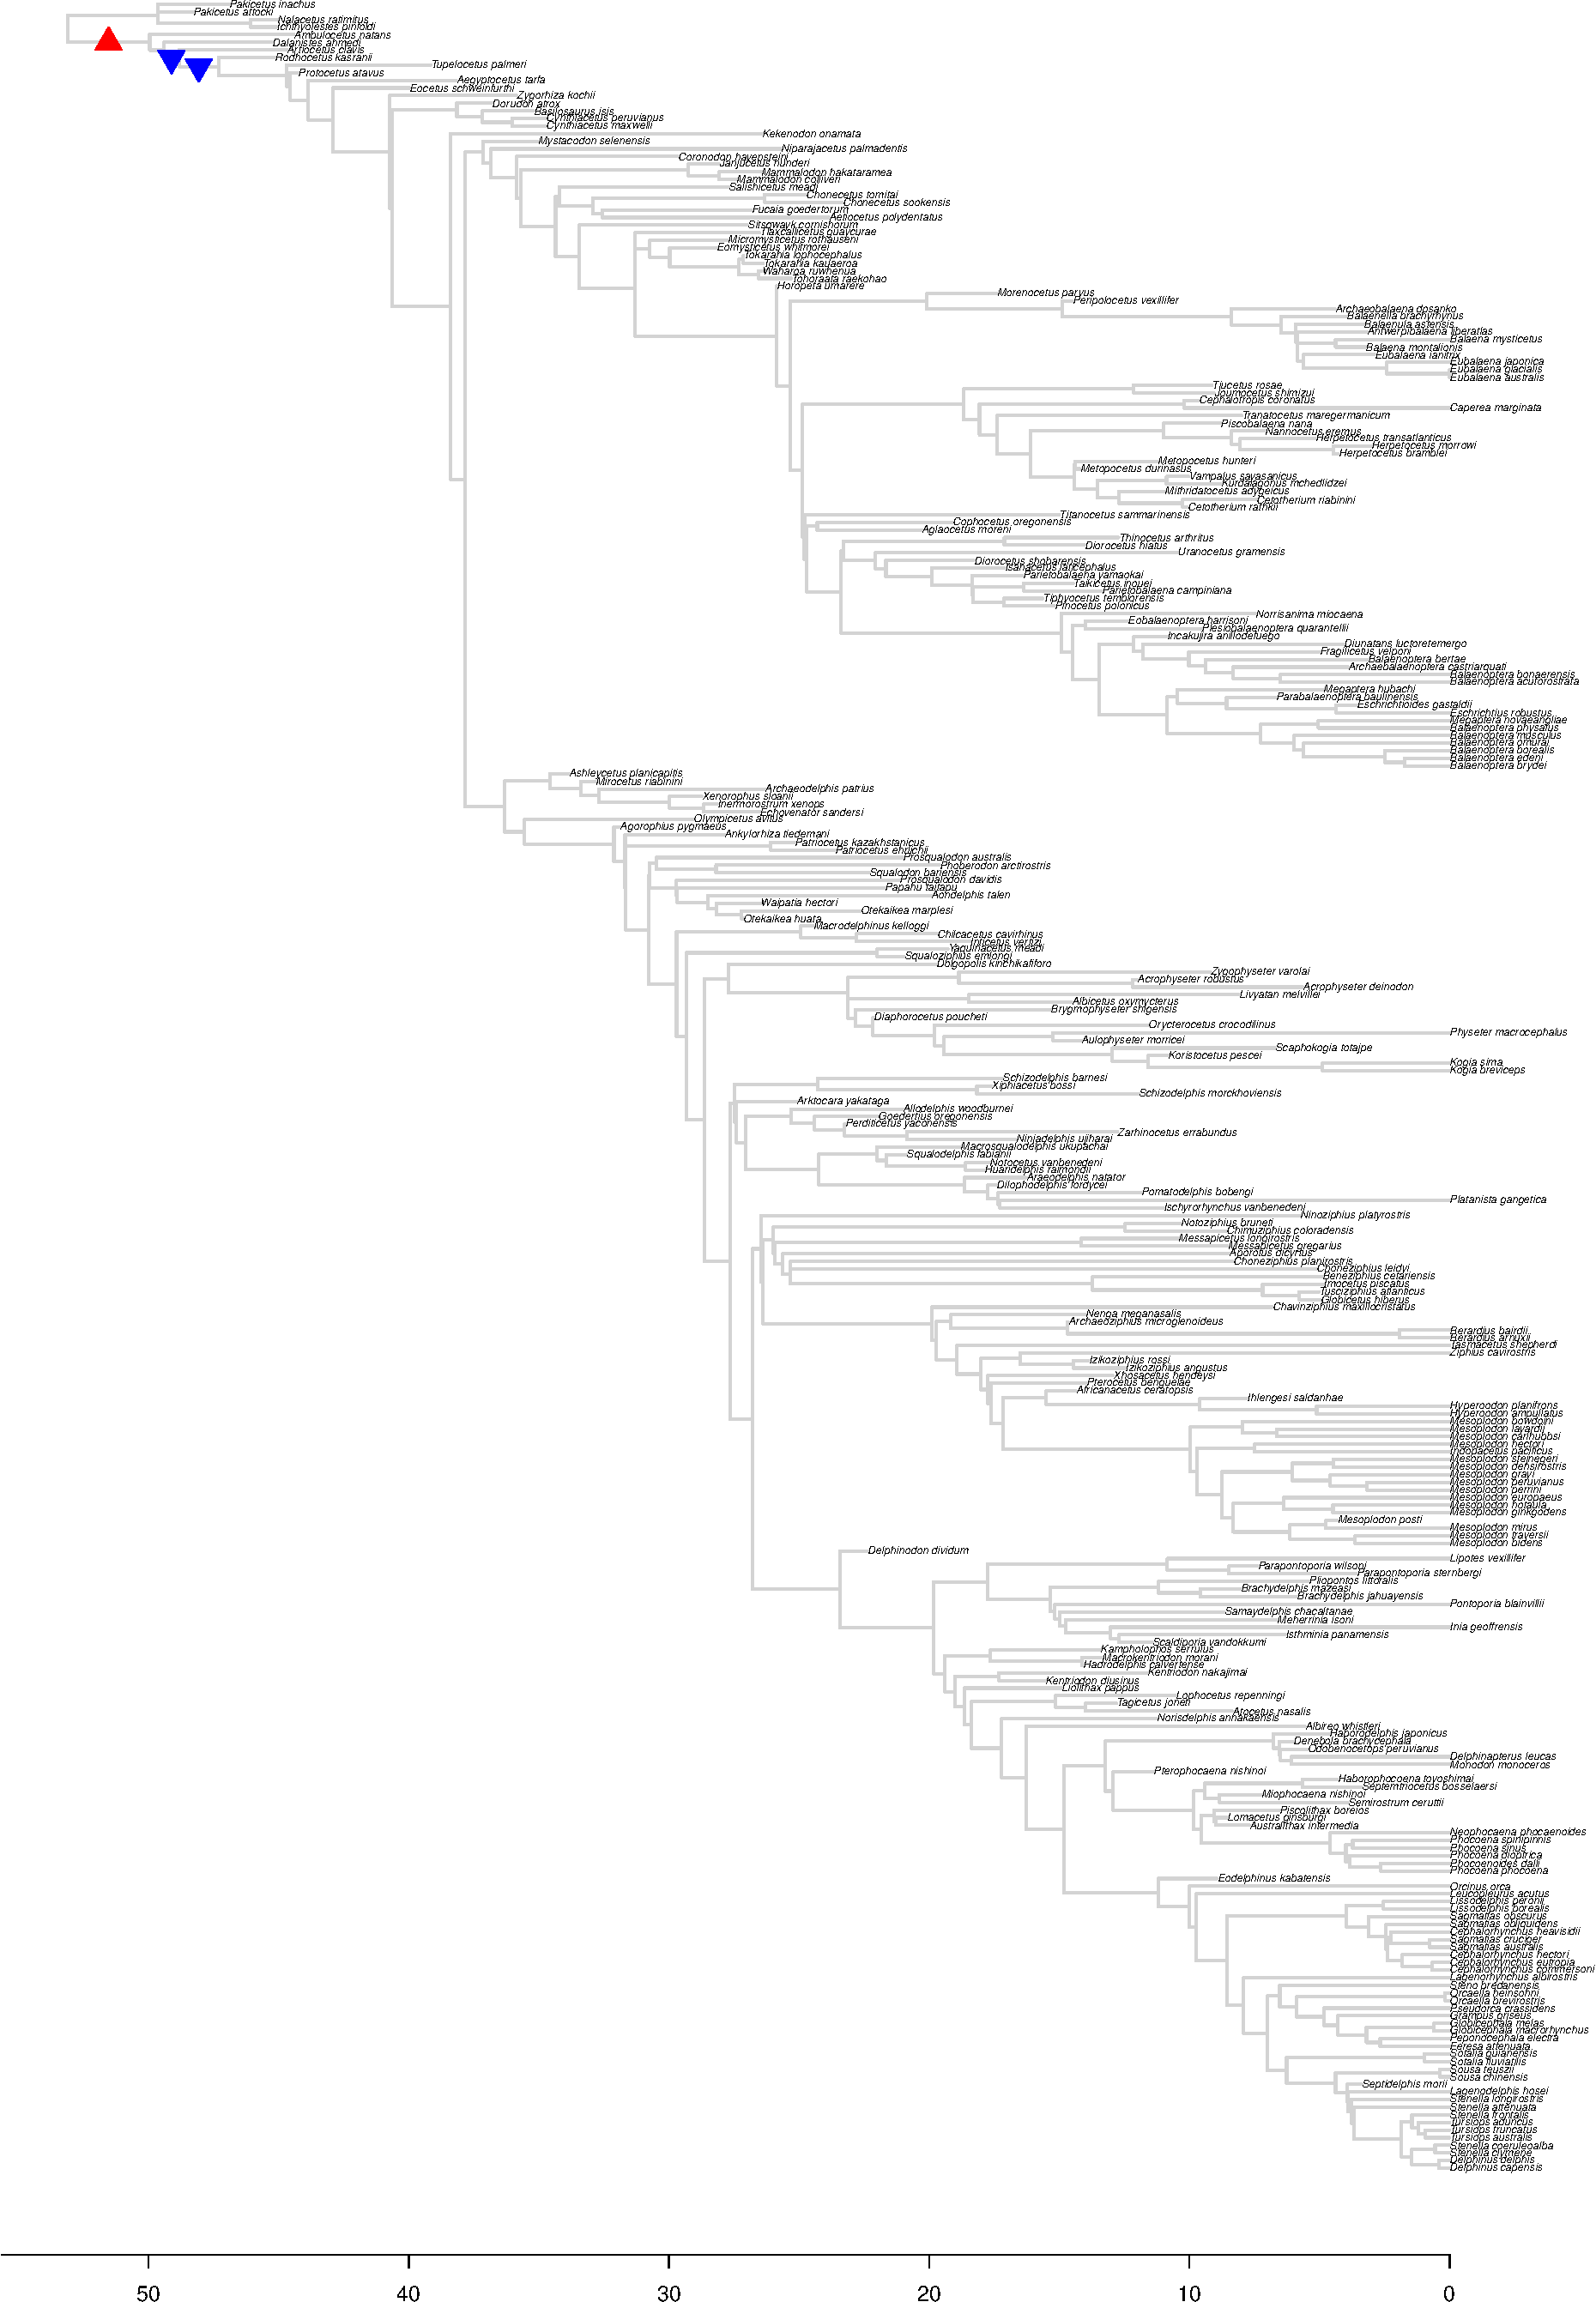
\includegraphics[width=0.8\textwidth]{img/plots-full-k5-1.pdf}
\caption{Results for \textit{bayou} fit for the \textit{Full} tree setting the average number of shifts in the prior distribution ($\lambda$) to 5. The triangles represent the position and direction of the shifts with posterior probability higher than 0.1, with upward triangles (in red) indicating increases in $\theta$, and downward triangles (in blue) indicating decreases in $\theta$.}
\label{fig:full-k5}
\end{figure}

\newpage

\begin{figure}[H]
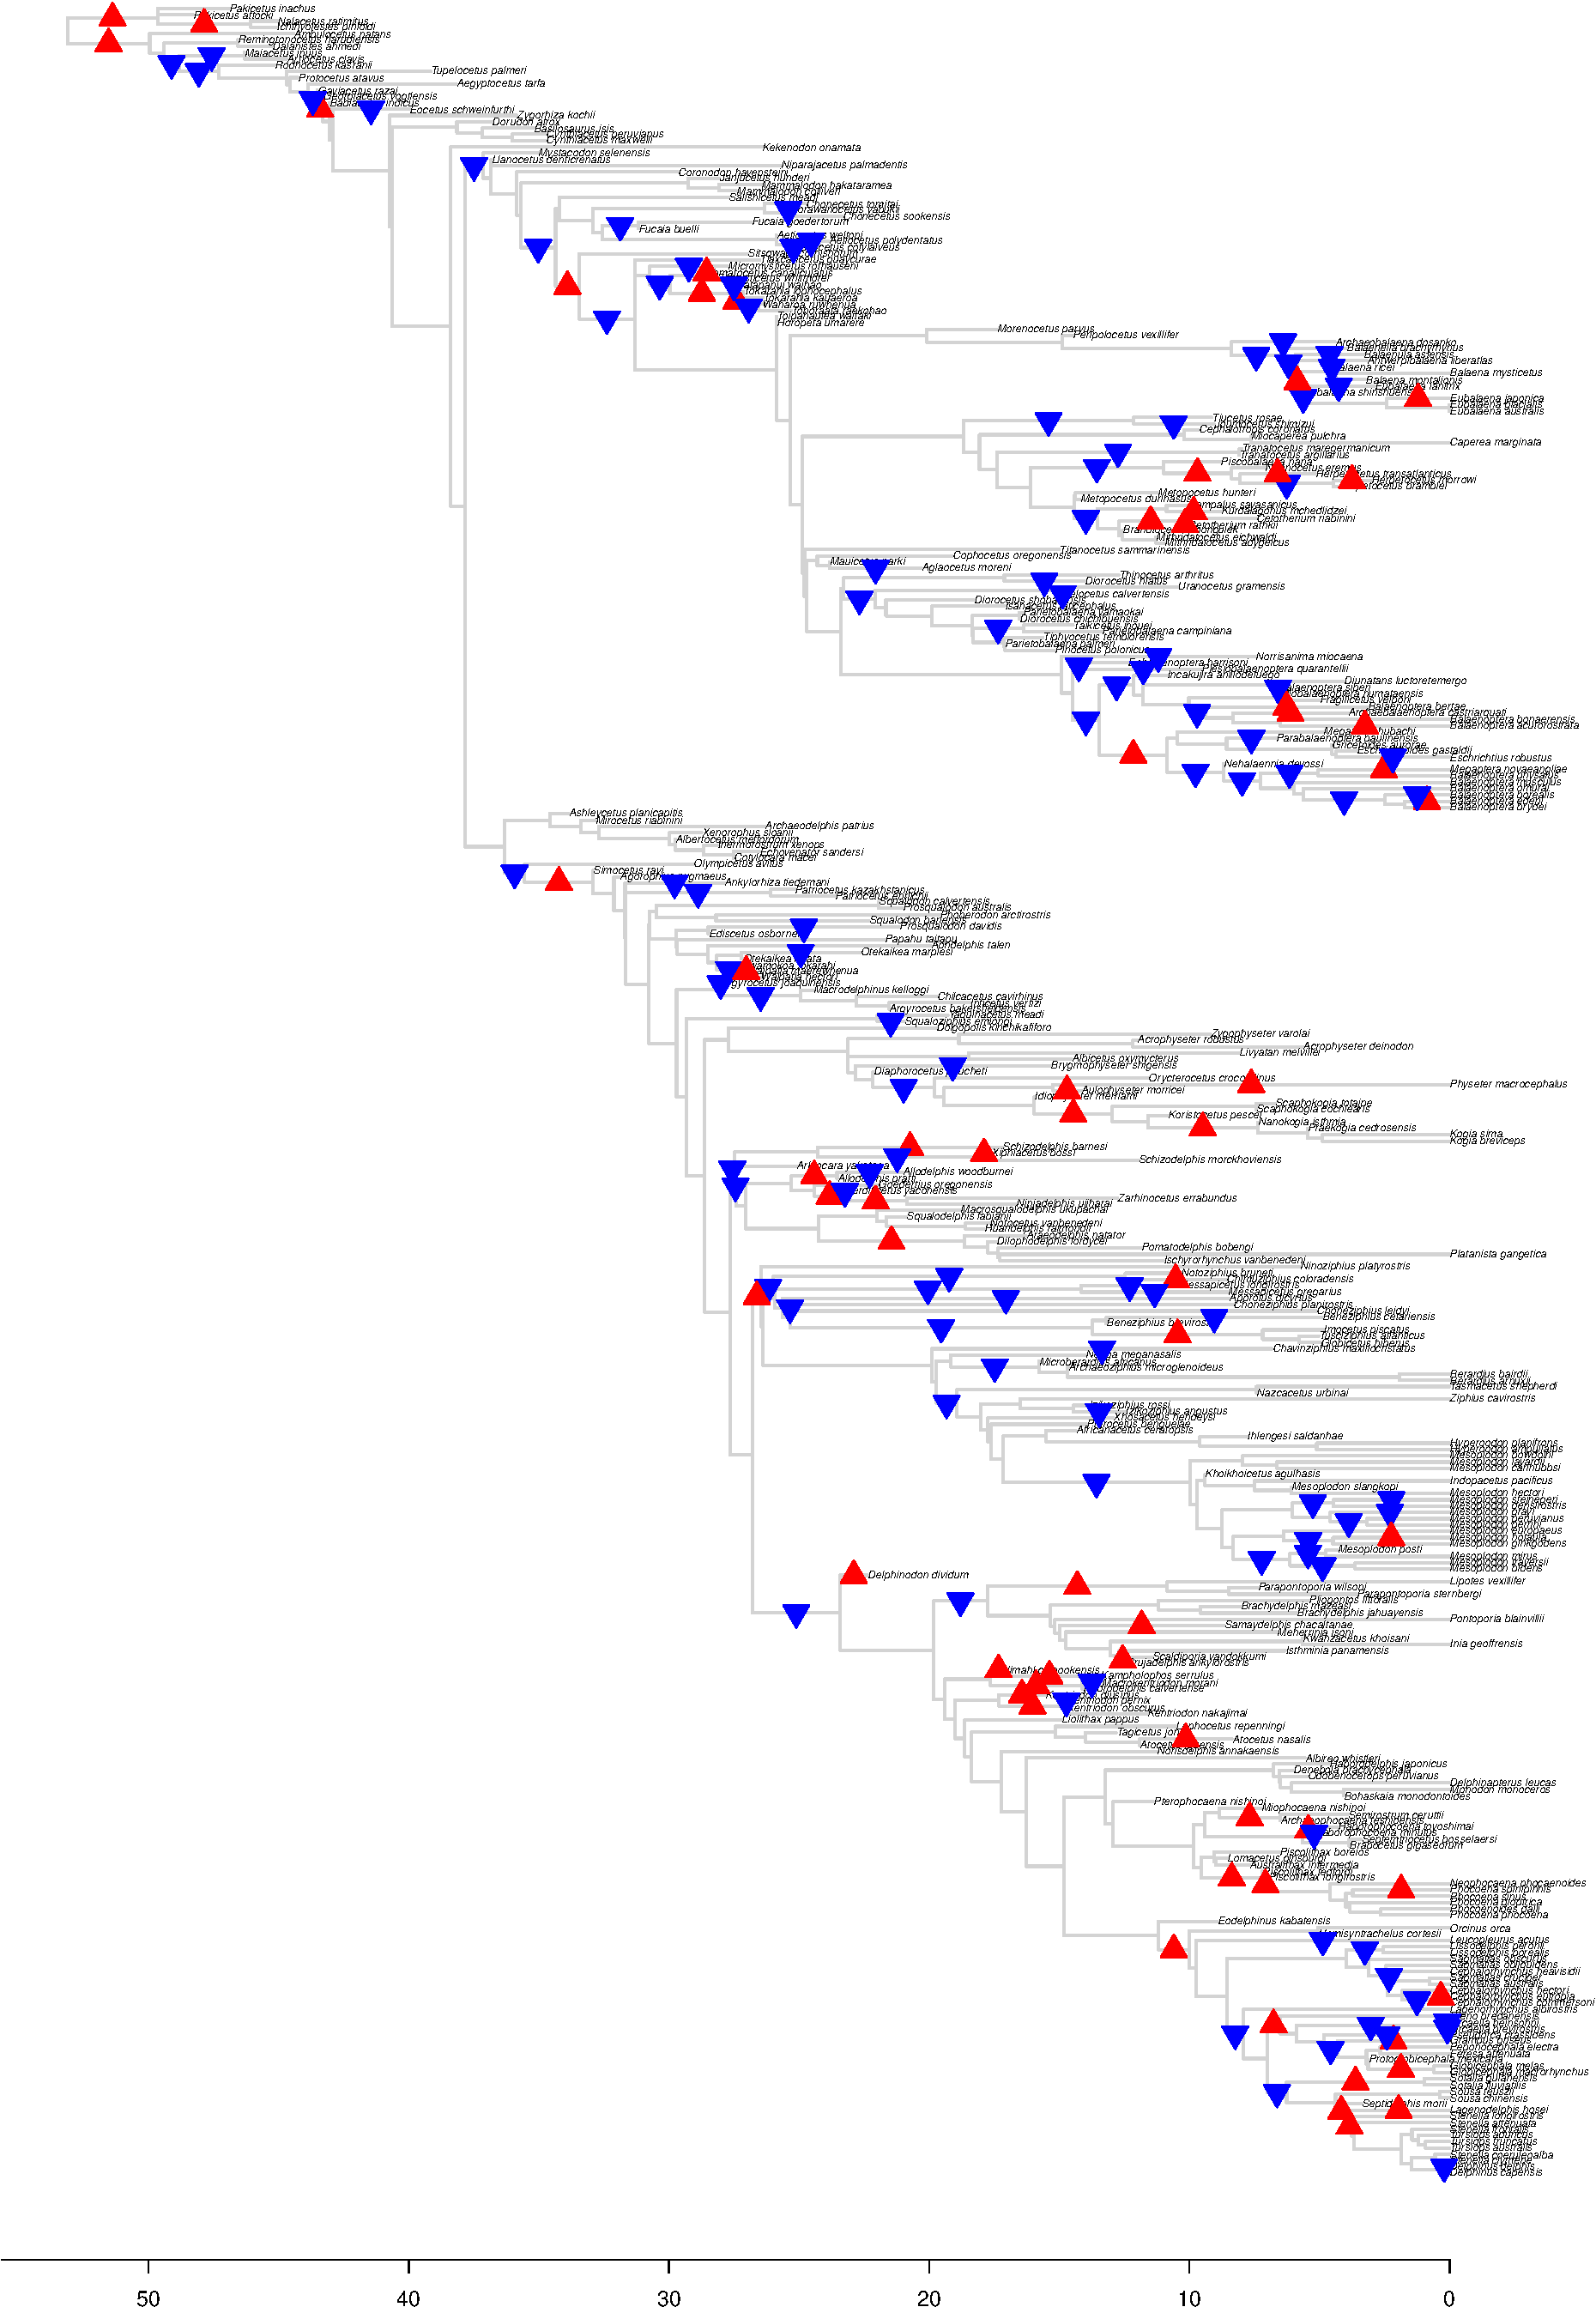
\includegraphics[width=0.9\textwidth]{img/plots-full-wZBL-k50-1.pdf}
\caption{Results for \textit{bayou} fit for the \textit{Full} tree setting the average number of shifts in the prior distribution ($\lambda$) to 50. The triangles represent the position and direction of the shifts with posterior probability higher than 0.1, with upward triangles (in red) indicating increases in $\theta$, and downward triangles (in blue) indicating decreases in $\theta$.}
\label{fig:full-k50}
\end{figure}

\newpage

\begin{figure}[H]
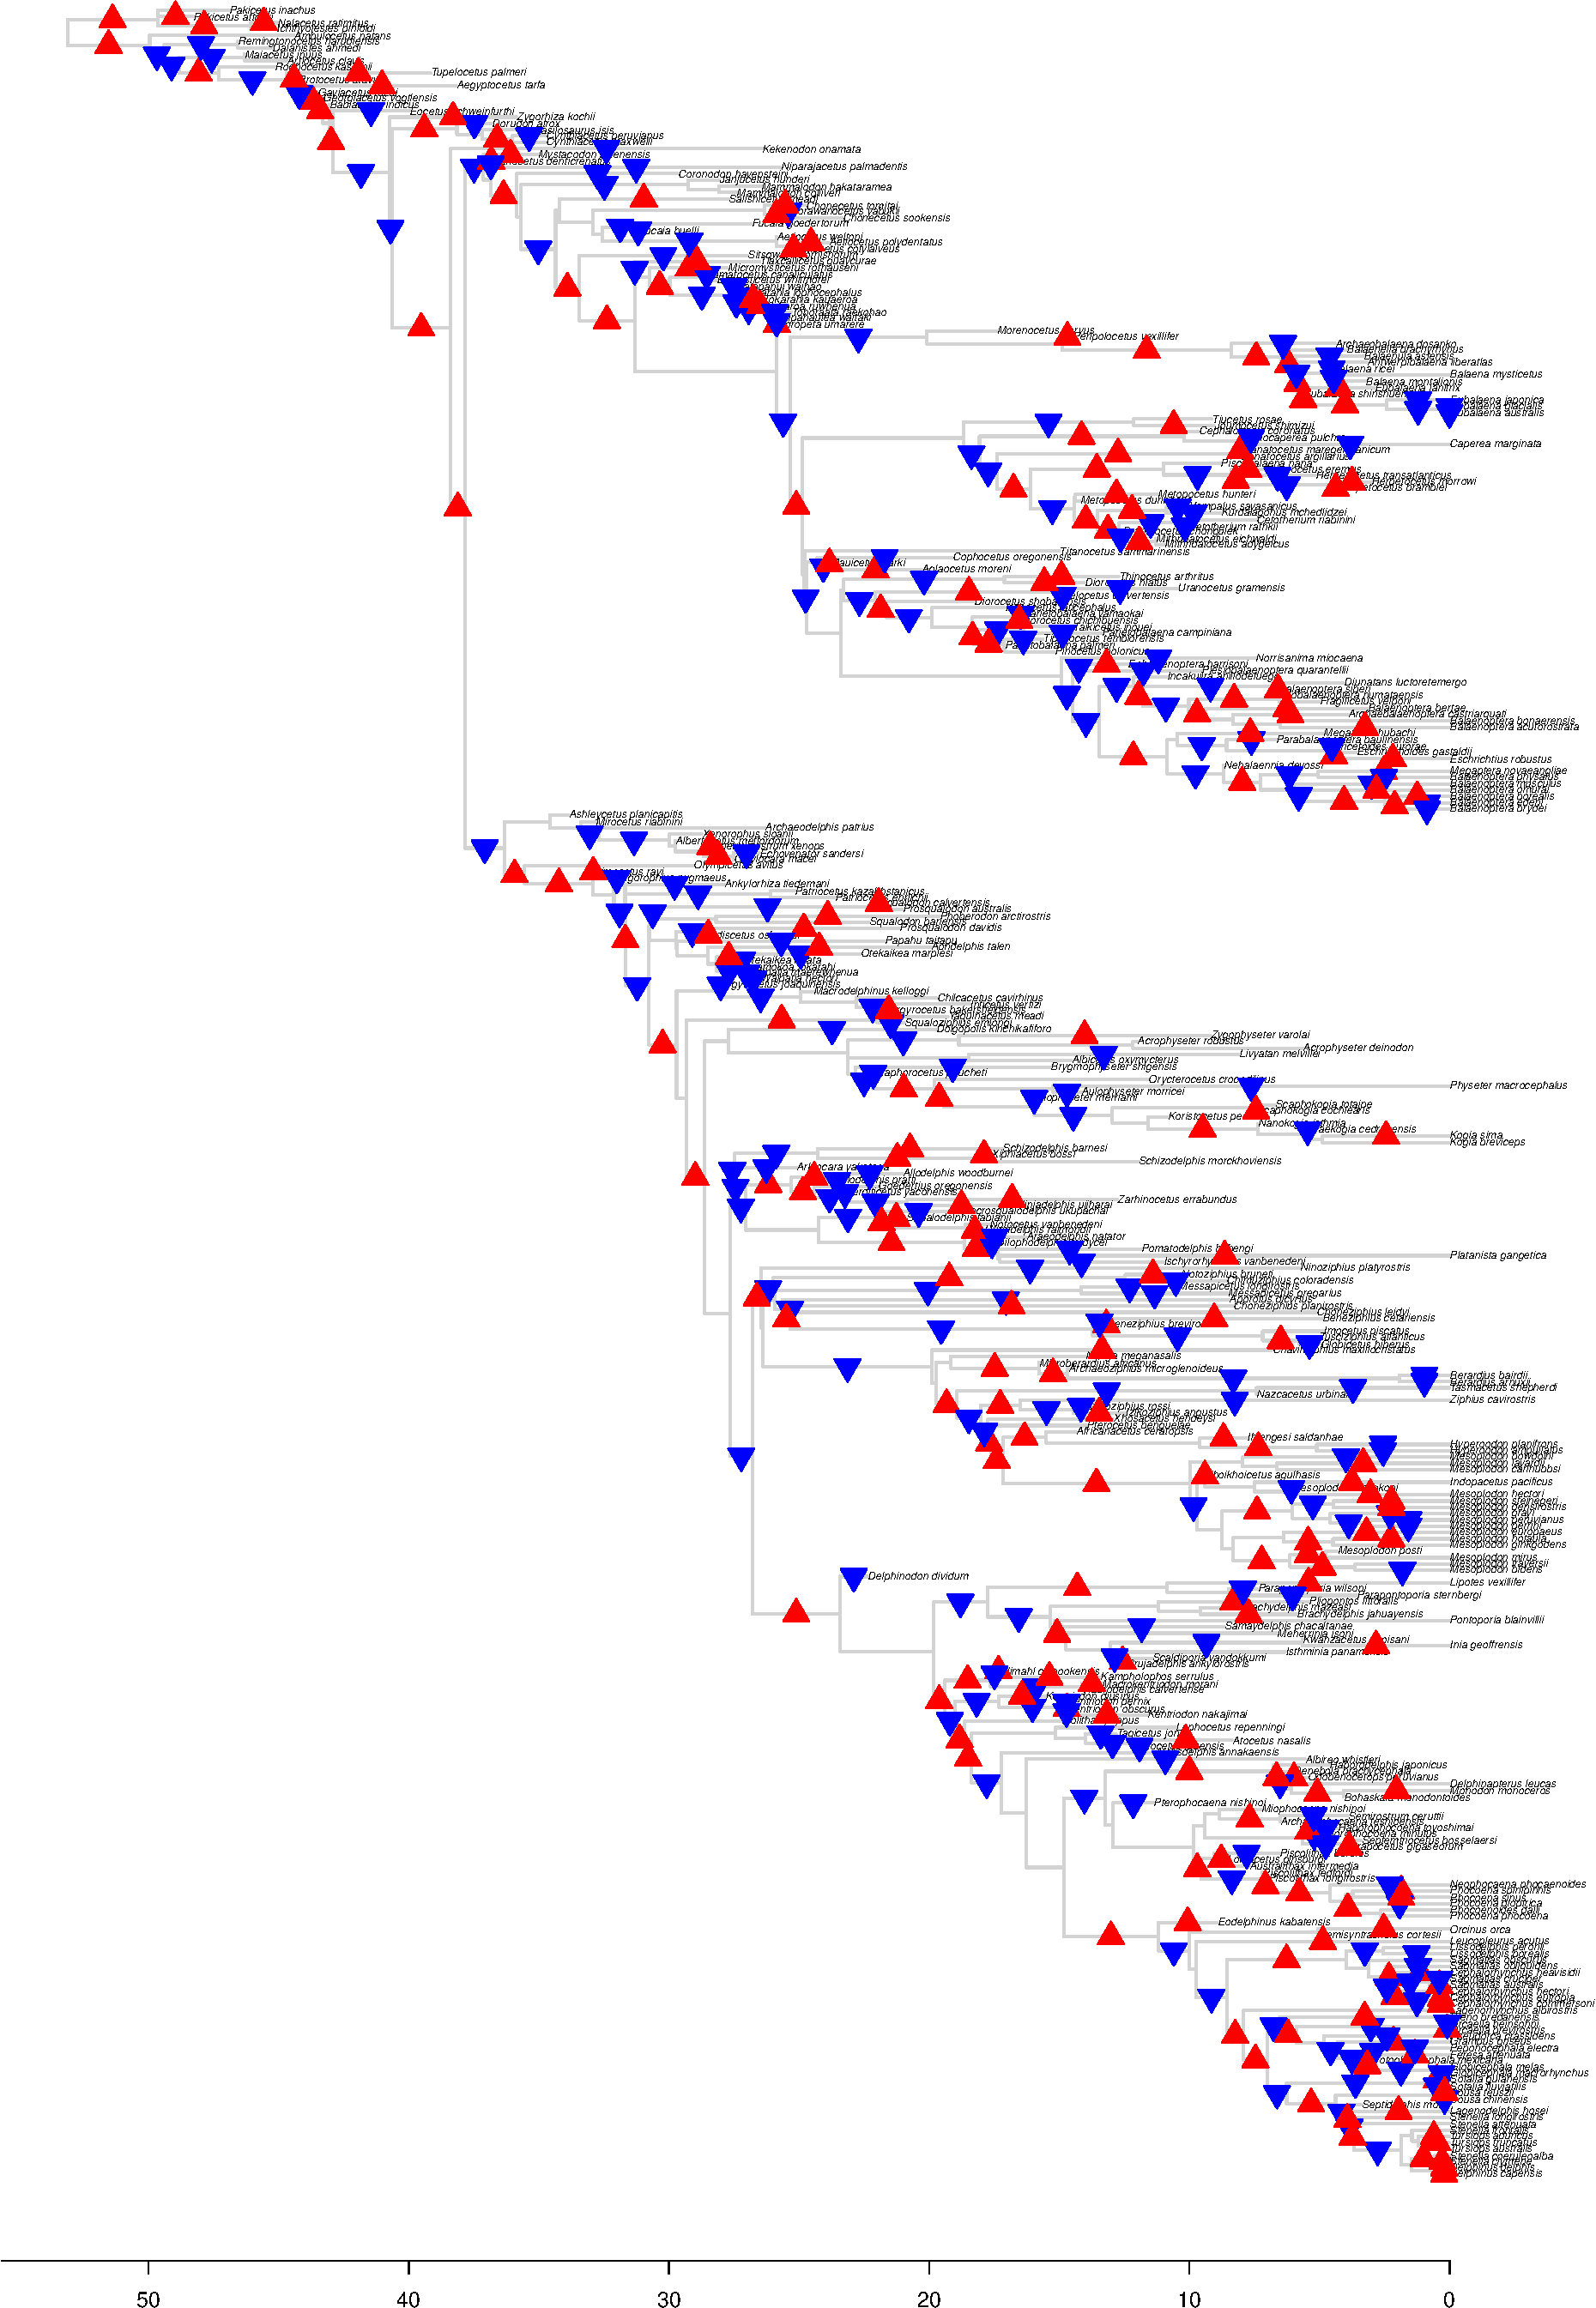
\includegraphics[width=0.9\textwidth]{img/plots-full-wZBL-k250-1.pdf}
\caption{Results for \textit{bayou} fit for the \textit{Full} tree setting the average number of shifts in the prior distribution ($\lambda$) to 250. The triangles represent the position and direction of the shifts with posterior probability higher than 0.1, with upward triangles (in red) indicating increases in $\theta$, and downward triangles (in blue) indicating decreases in $\theta$.}
\label{fig:full-k250}
\end{figure}

\newpage

\begin{figure}[H]
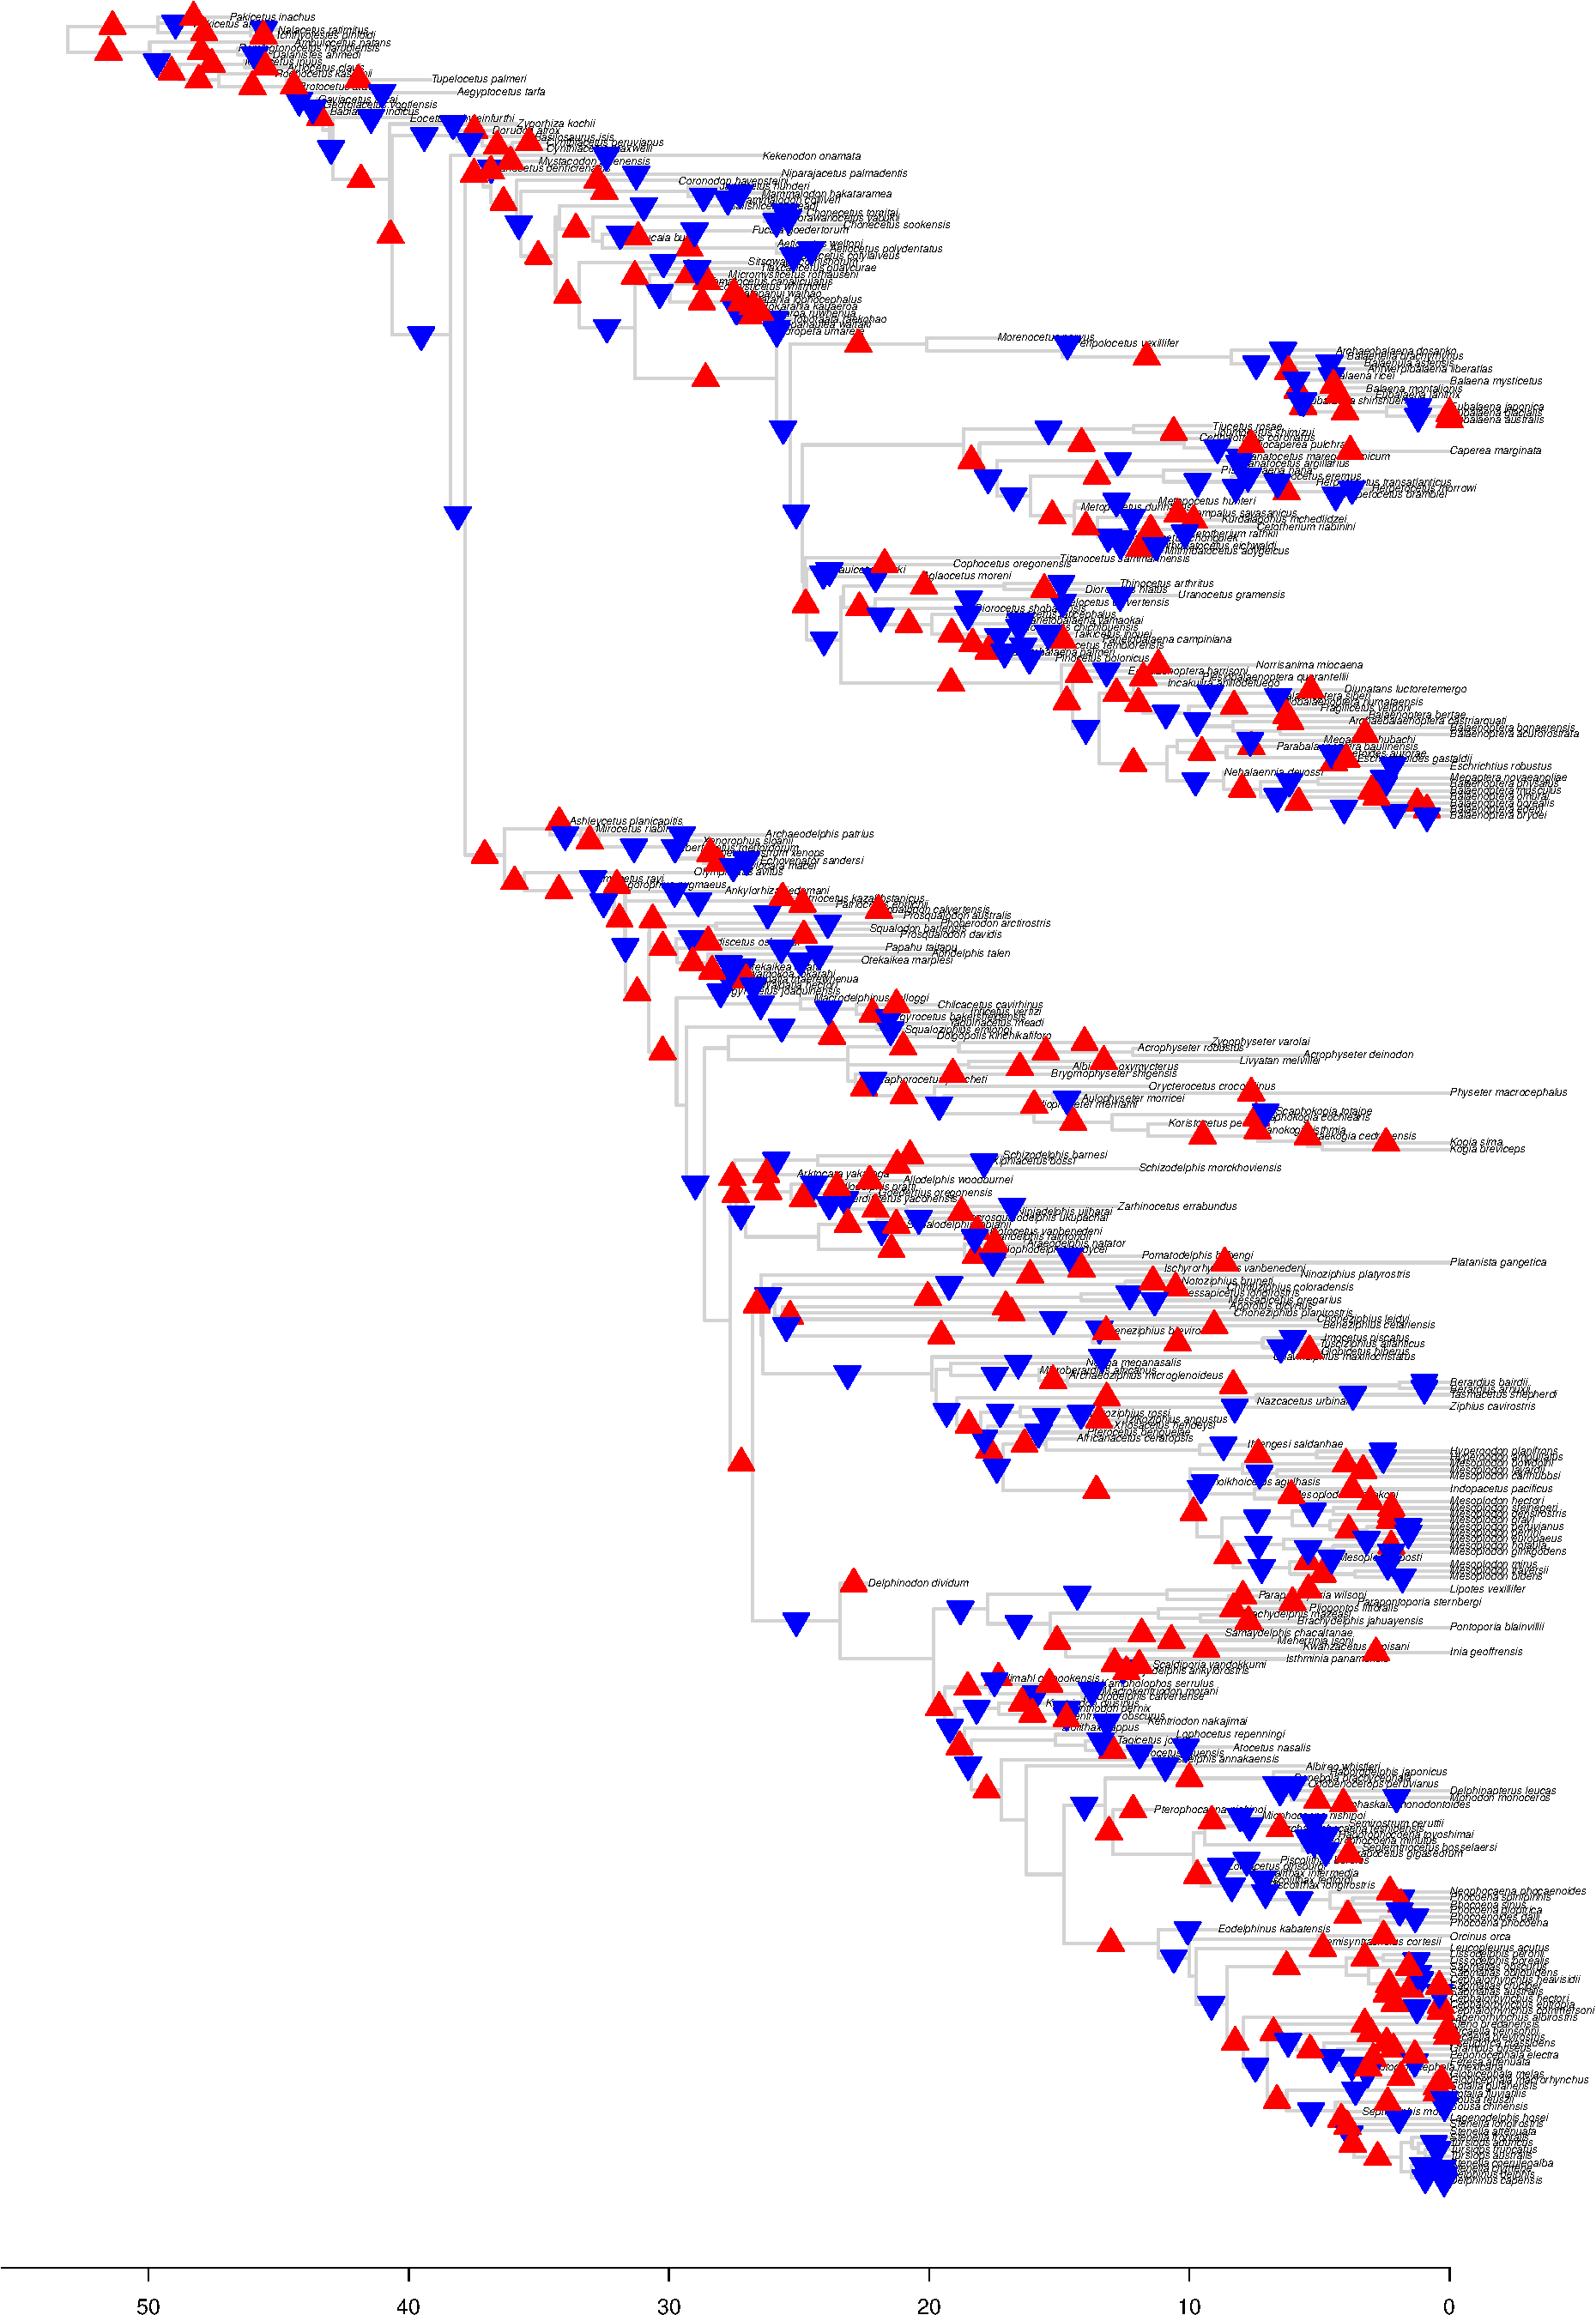
\includegraphics[width=0.9\textwidth]{img/plots-full-wZBL-k500-1.pdf}
\caption{Results for \textit{bayou} fit for the \textit{Full} tree setting the average number of shifts in the prior distribution ($\lambda$) to 500. The triangles represent the position and direction of the shifts with posterior probability higher than 0.1, with upward triangles (in red) indicating increases in $\theta$, and downward triangles (in blue) indicating decreases in $\theta$.}
\label{fig:full-k500}
\end{figure}

%---------------------------------------------------------------------
\subsubsection{\textit{No Archaeoceti} tree}
%---------------------------------------------------------------------

\begin{figure}[H]
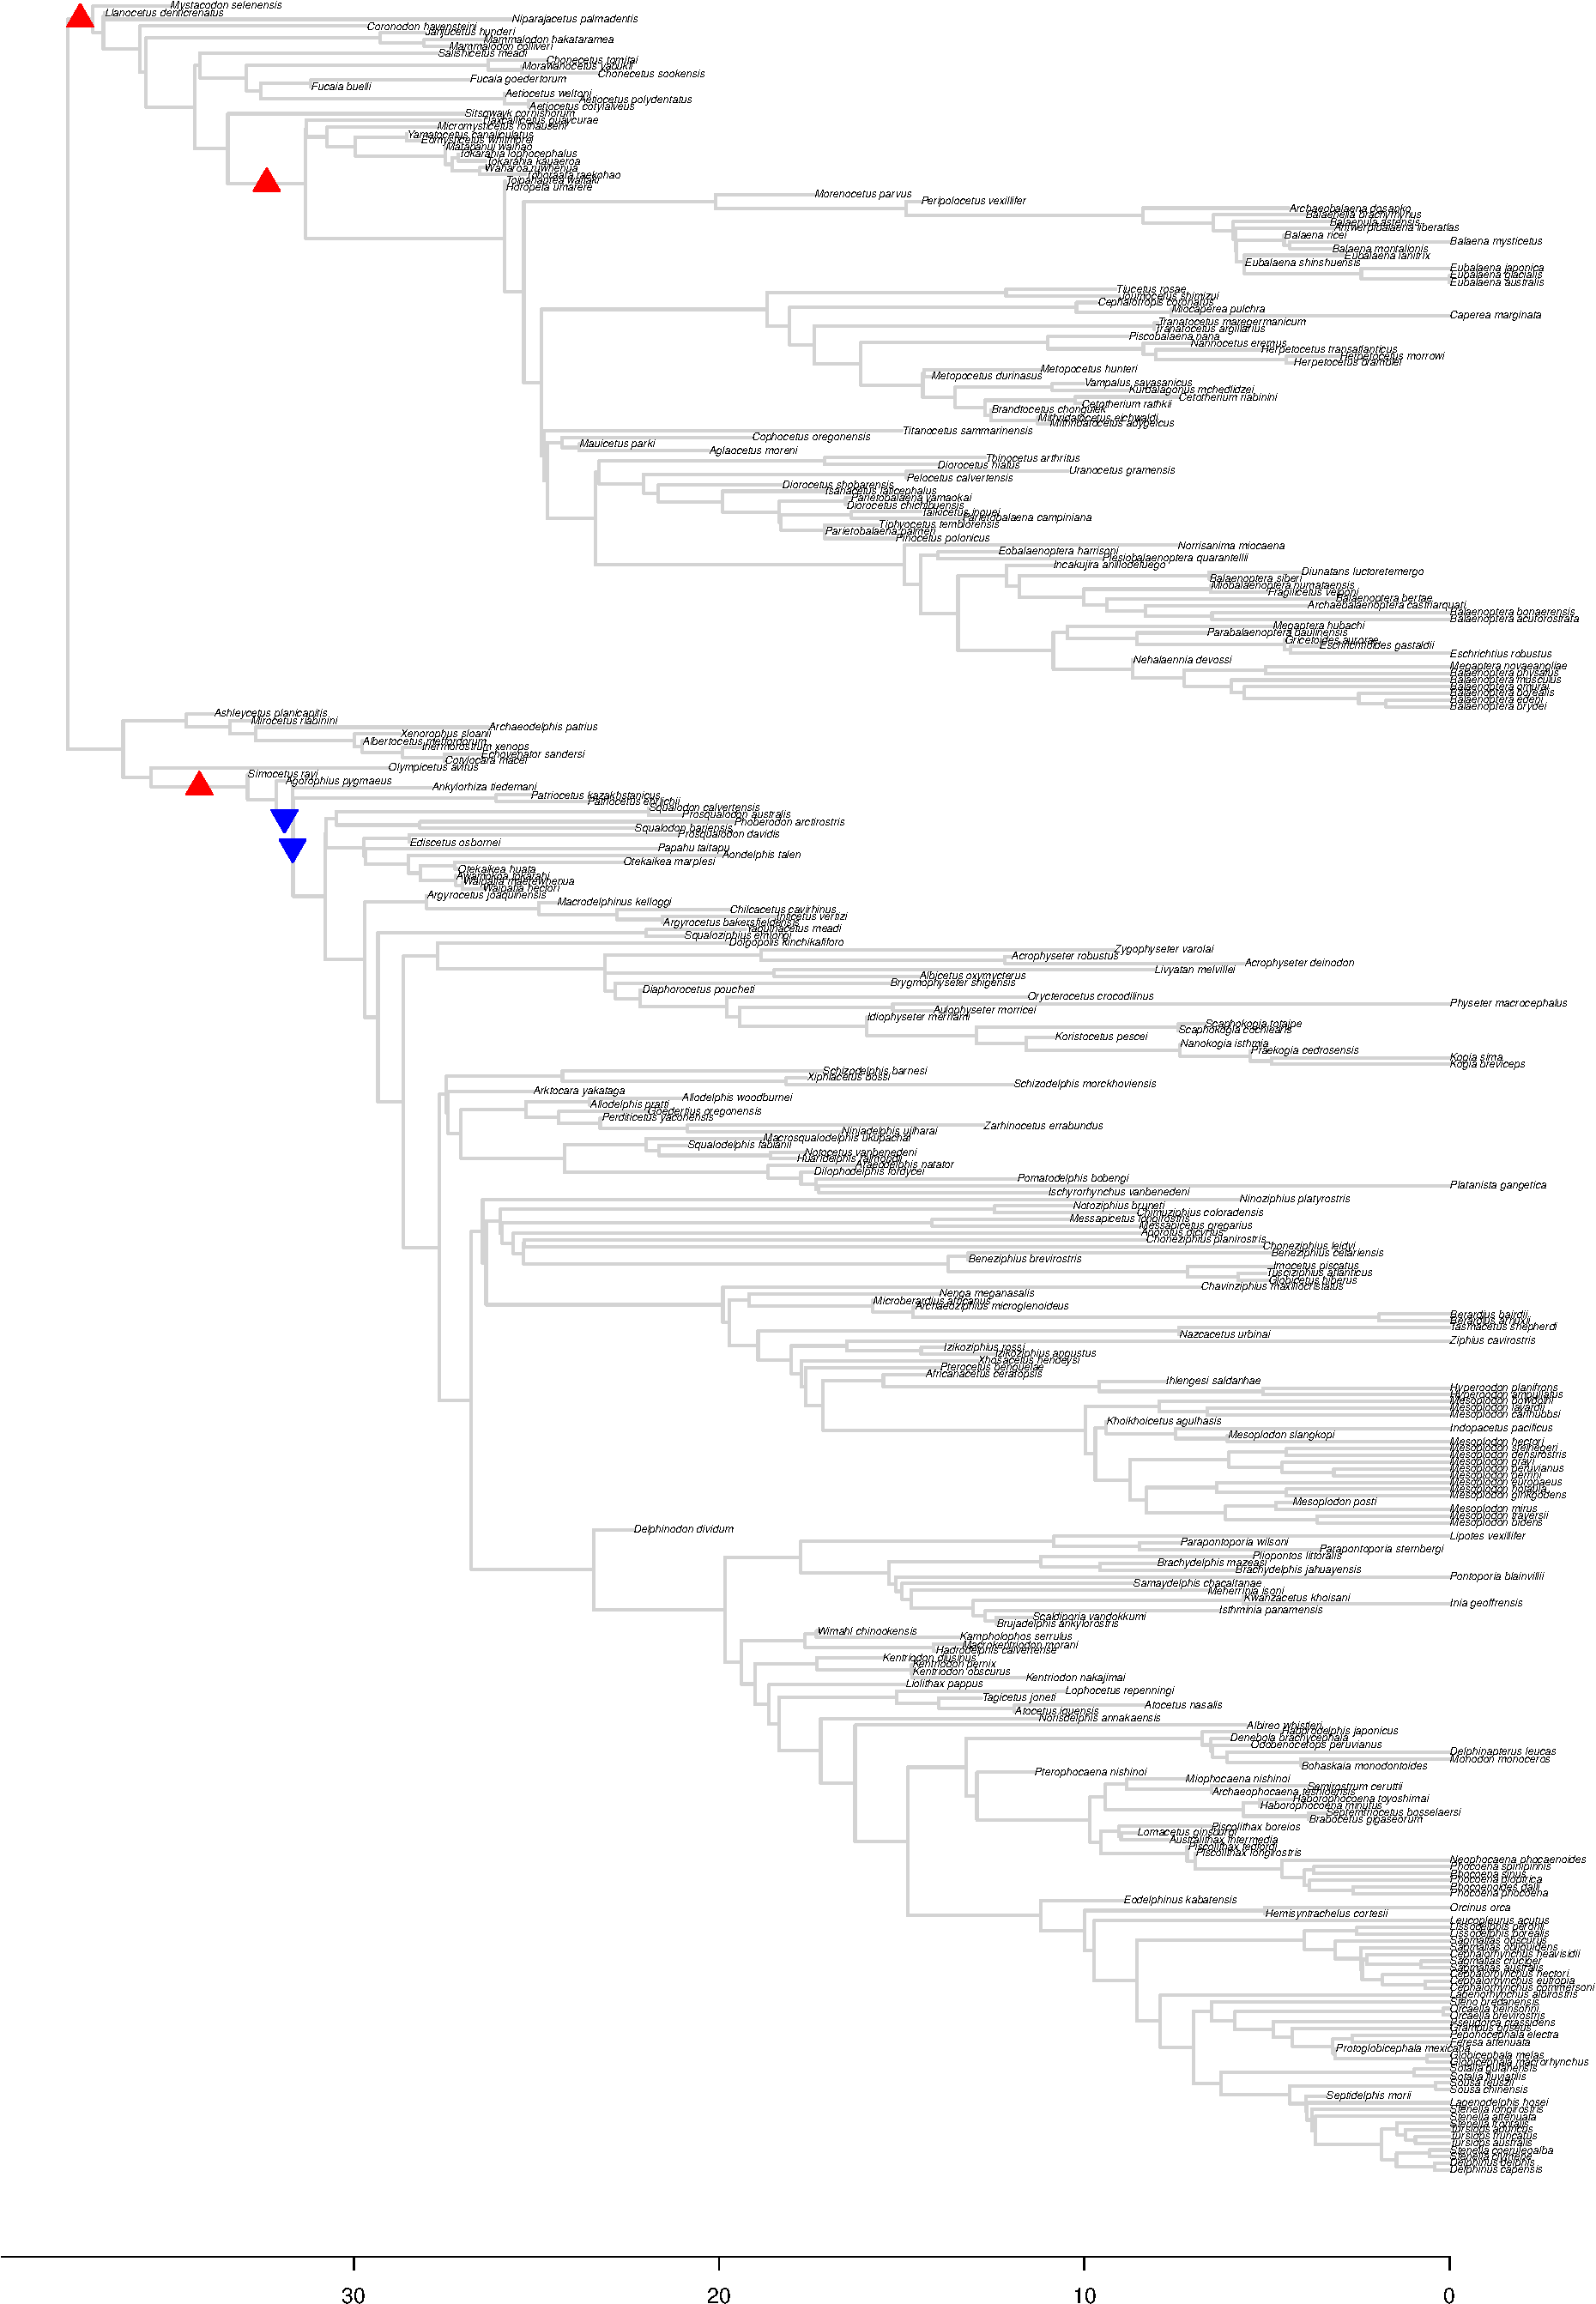
\includegraphics[width=0.9\textwidth]{img/plots-noarchaeo-wZBL-k5-1.pdf}
\caption{Results for \textit{bayou} fit for the \textit{No Archaeoceti} tree setting the average number of shifts in the prior distribution ($\lambda$) to 5. The triangles represent the position and direction of the shifts with posterior probability higher than 0.1, with upward triangles (in red) indicating increases in $\theta$, and downward triangles (in blue) indicating decreases in $\theta$.}
\label{fig:noarchaeo-k5}
\end{figure}

\newpage

\begin{figure}[H]
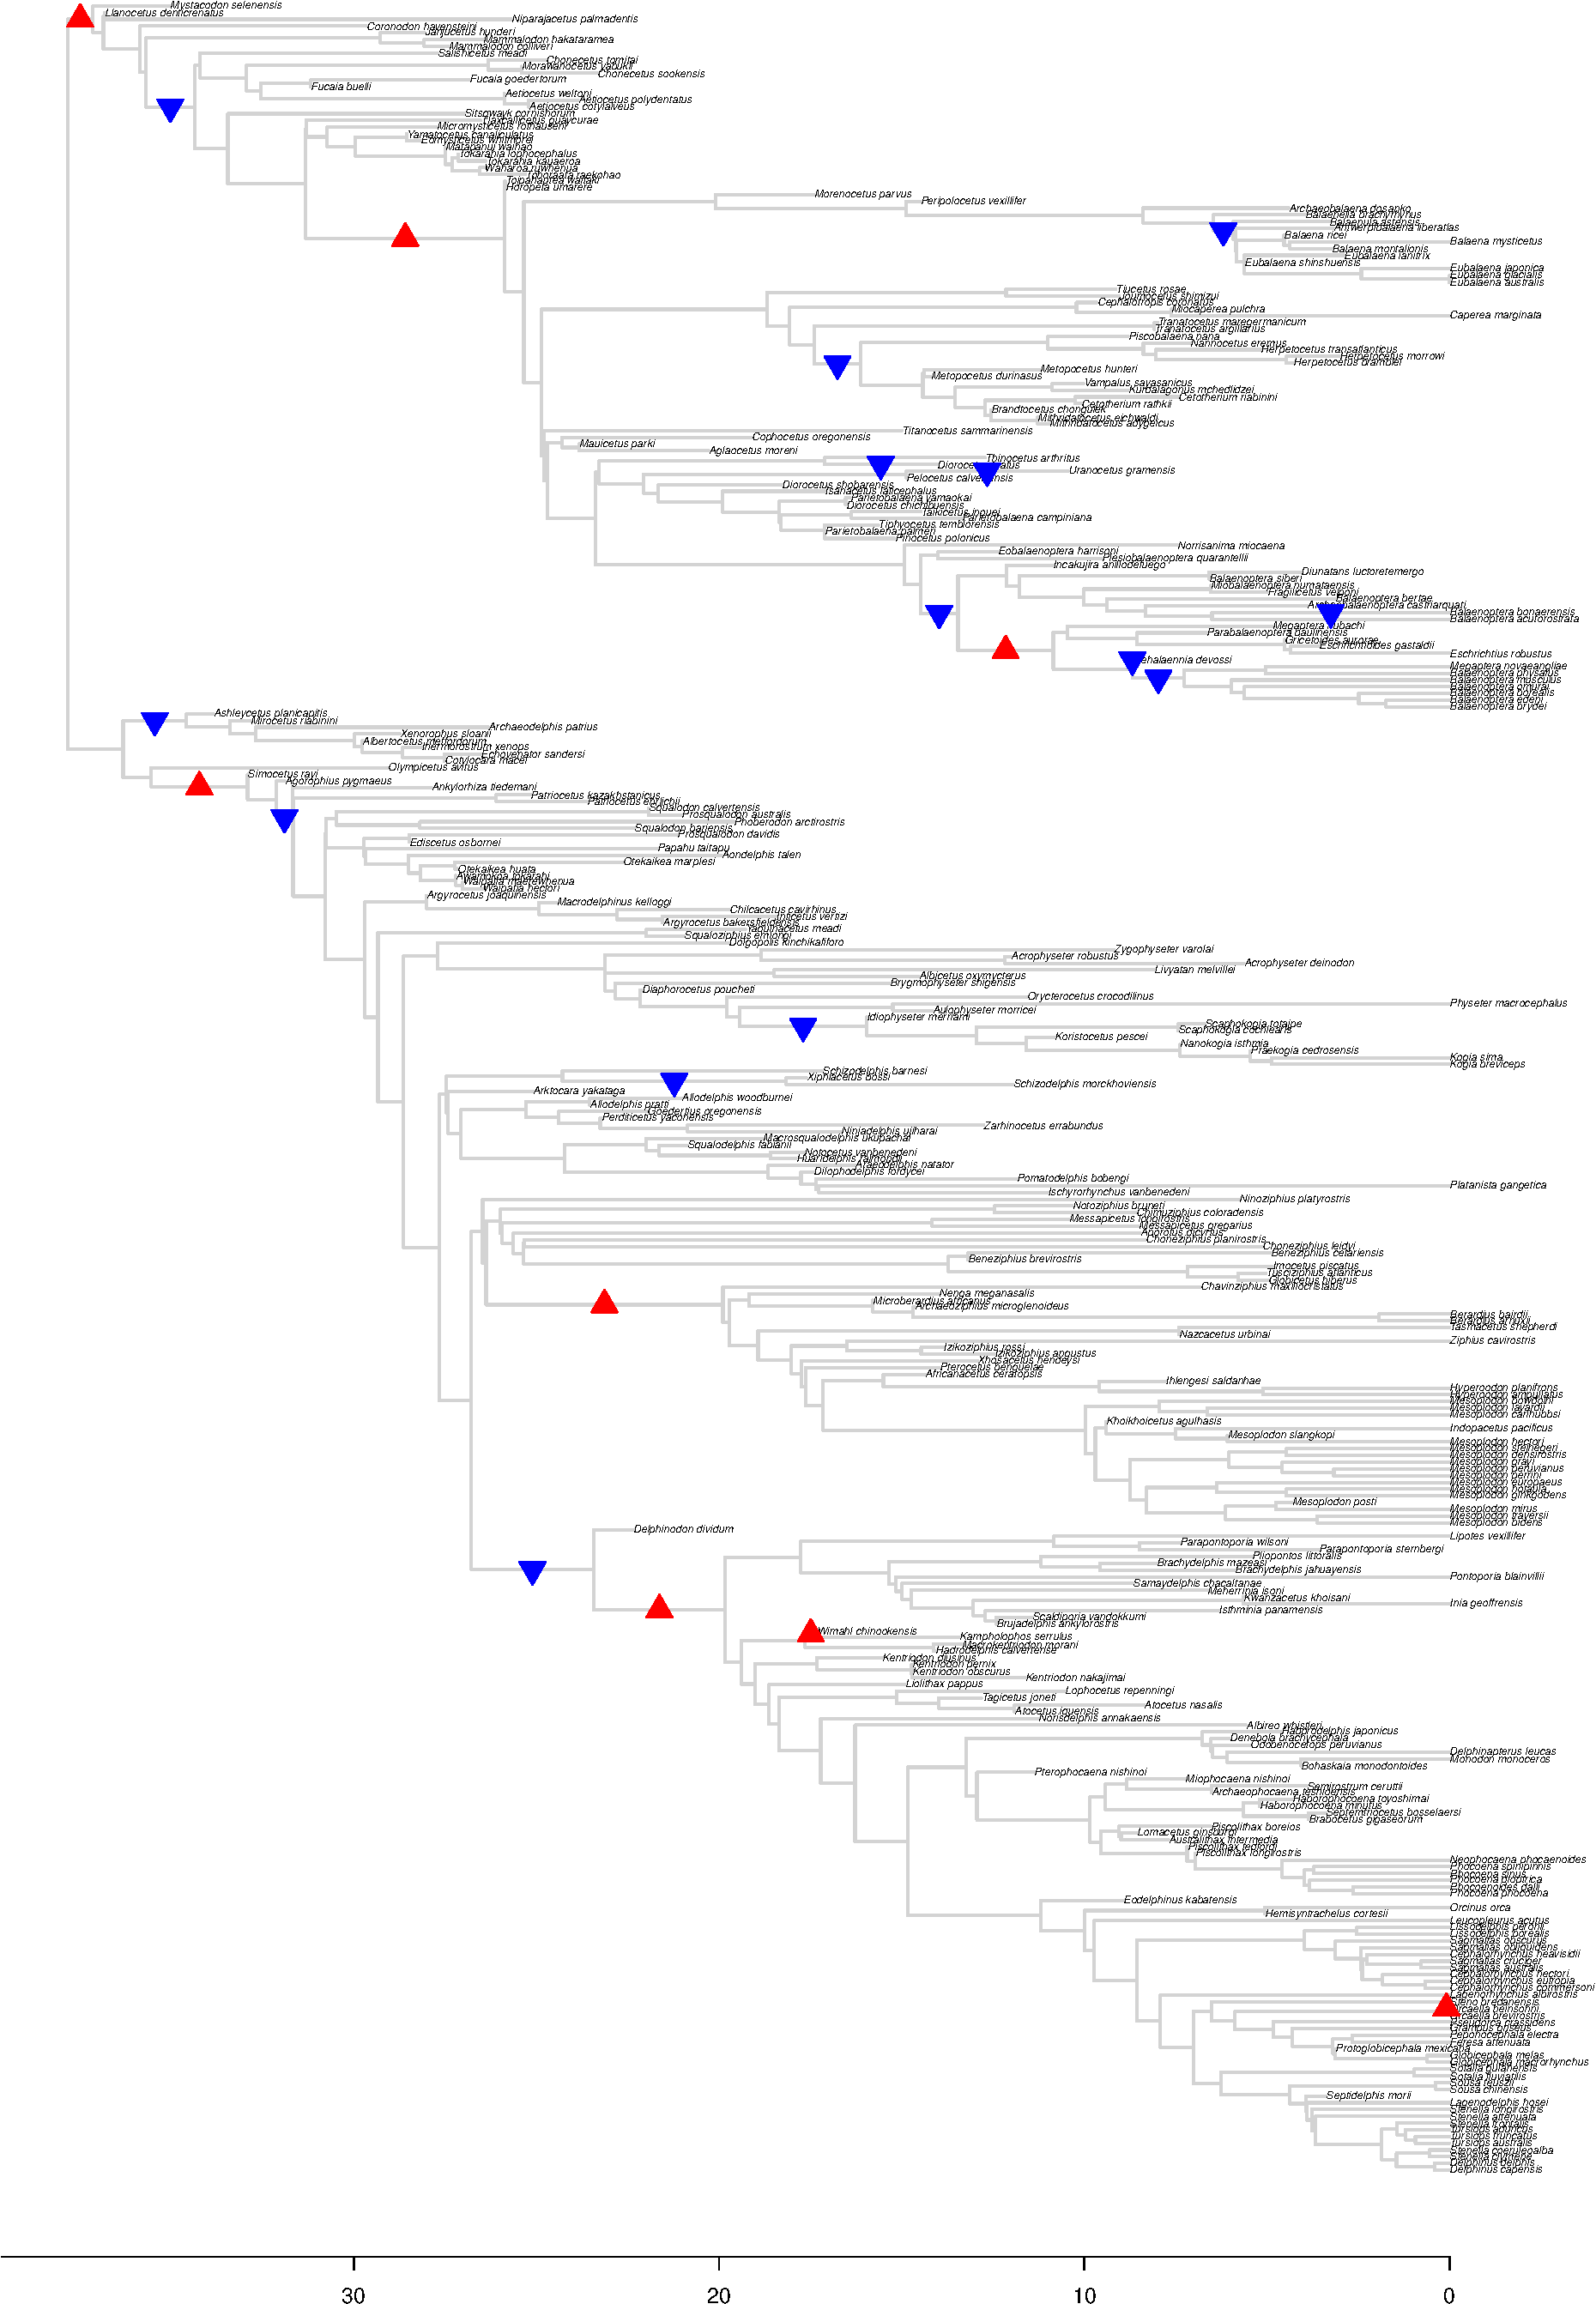
\includegraphics[width=0.9\textwidth]{img/plots-noarchaeo-wZBL-k15-1.pdf}
\caption{Results for \textit{bayou} fit for the \textit{No Archaeoceti} tree setting the average number of shifts in the prior distribution ($\lambda$) to 15. The triangles represent the position and direction of the shifts with posterior probability higher than 0.1, with upward triangles (in red) indicating increases in $\theta$, and downward triangles (in blue) indicating decreases in $\theta$.}
\label{fig:noarchaeo-k15}
\end{figure}

\newpage

\begin{figure}[H]
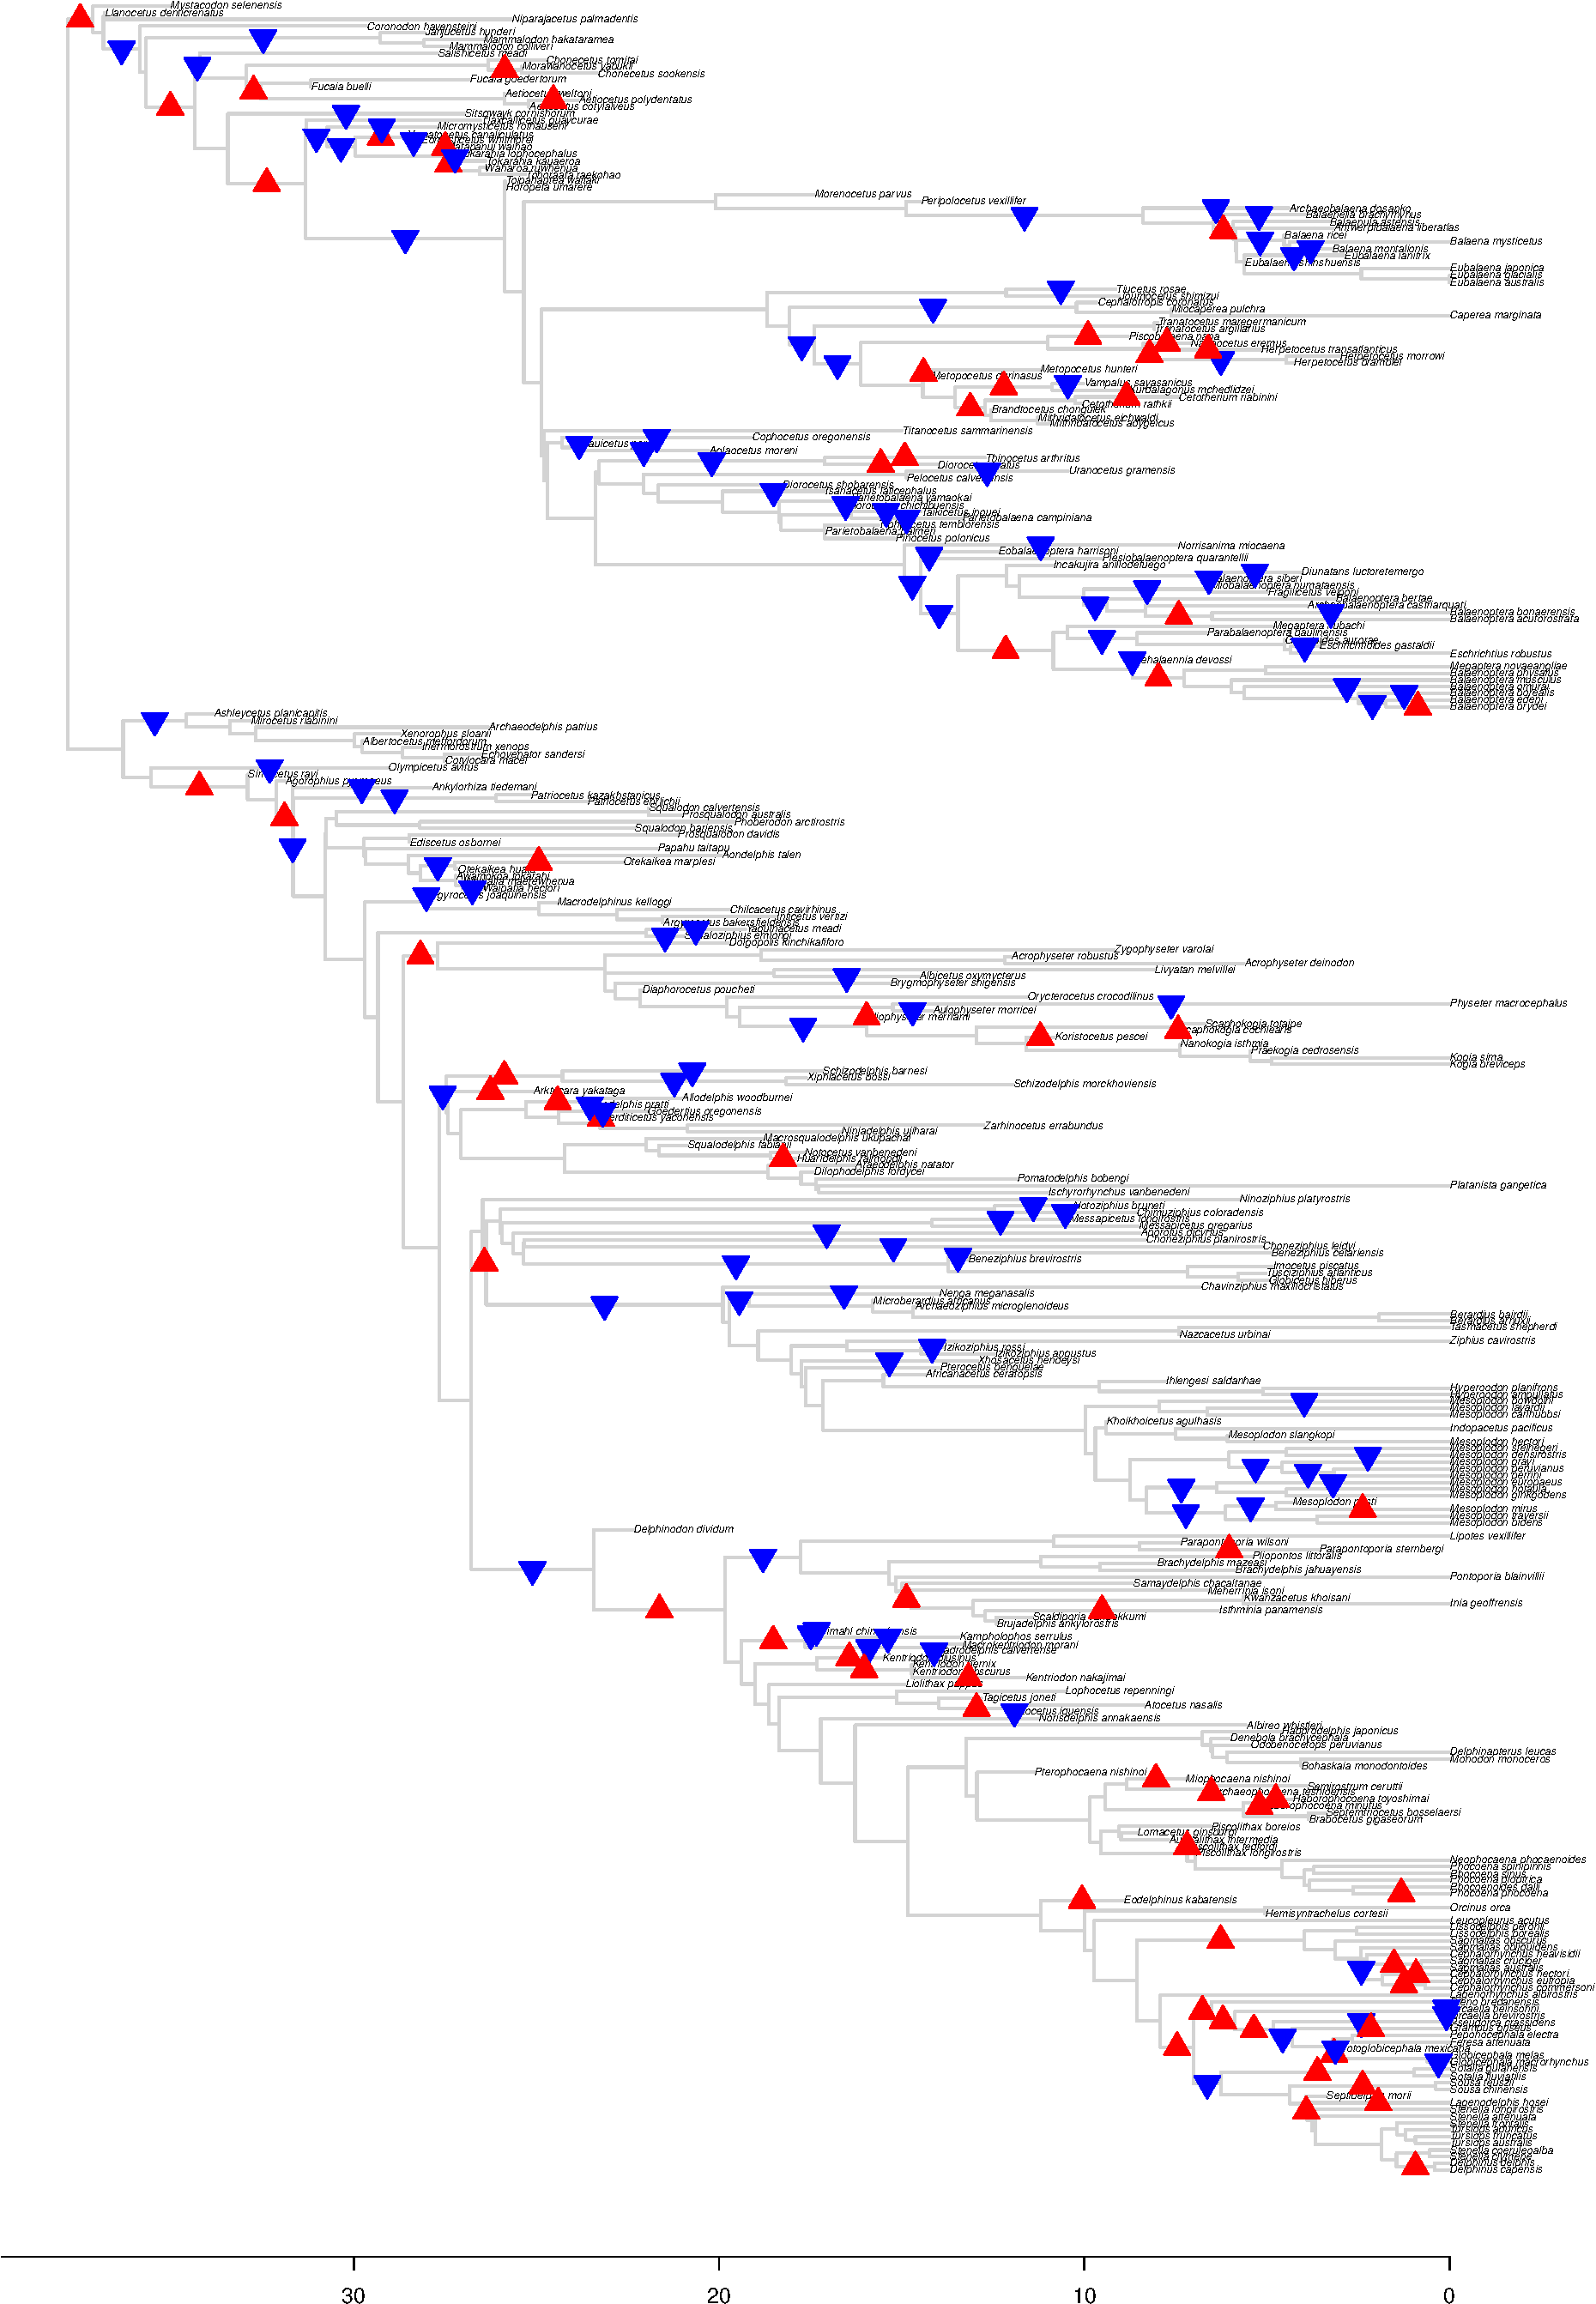
\includegraphics[width=0.9\textwidth]{img/plots-noarchaeo-wZBL-k50-1.pdf}
\caption{Results for \textit{bayou} fit for the \textit{No Archaeoceti} tree setting the average number of shifts in the prior distribution ($\lambda$) to 50. The triangles represent the position and direction of the shifts with posterior probability higher than 0.1, with upward triangles (in red) indicating increases in $\theta$, and downward triangles (in blue) indicating decreases in $\theta$.}
\label{fig:noarchaeo-k50}
\end{figure}

%---------------------------------------------------------------------
\subsubsection{\textit{No Extant} tree}
%---------------------------------------------------------------------

\begin{figure}[H]
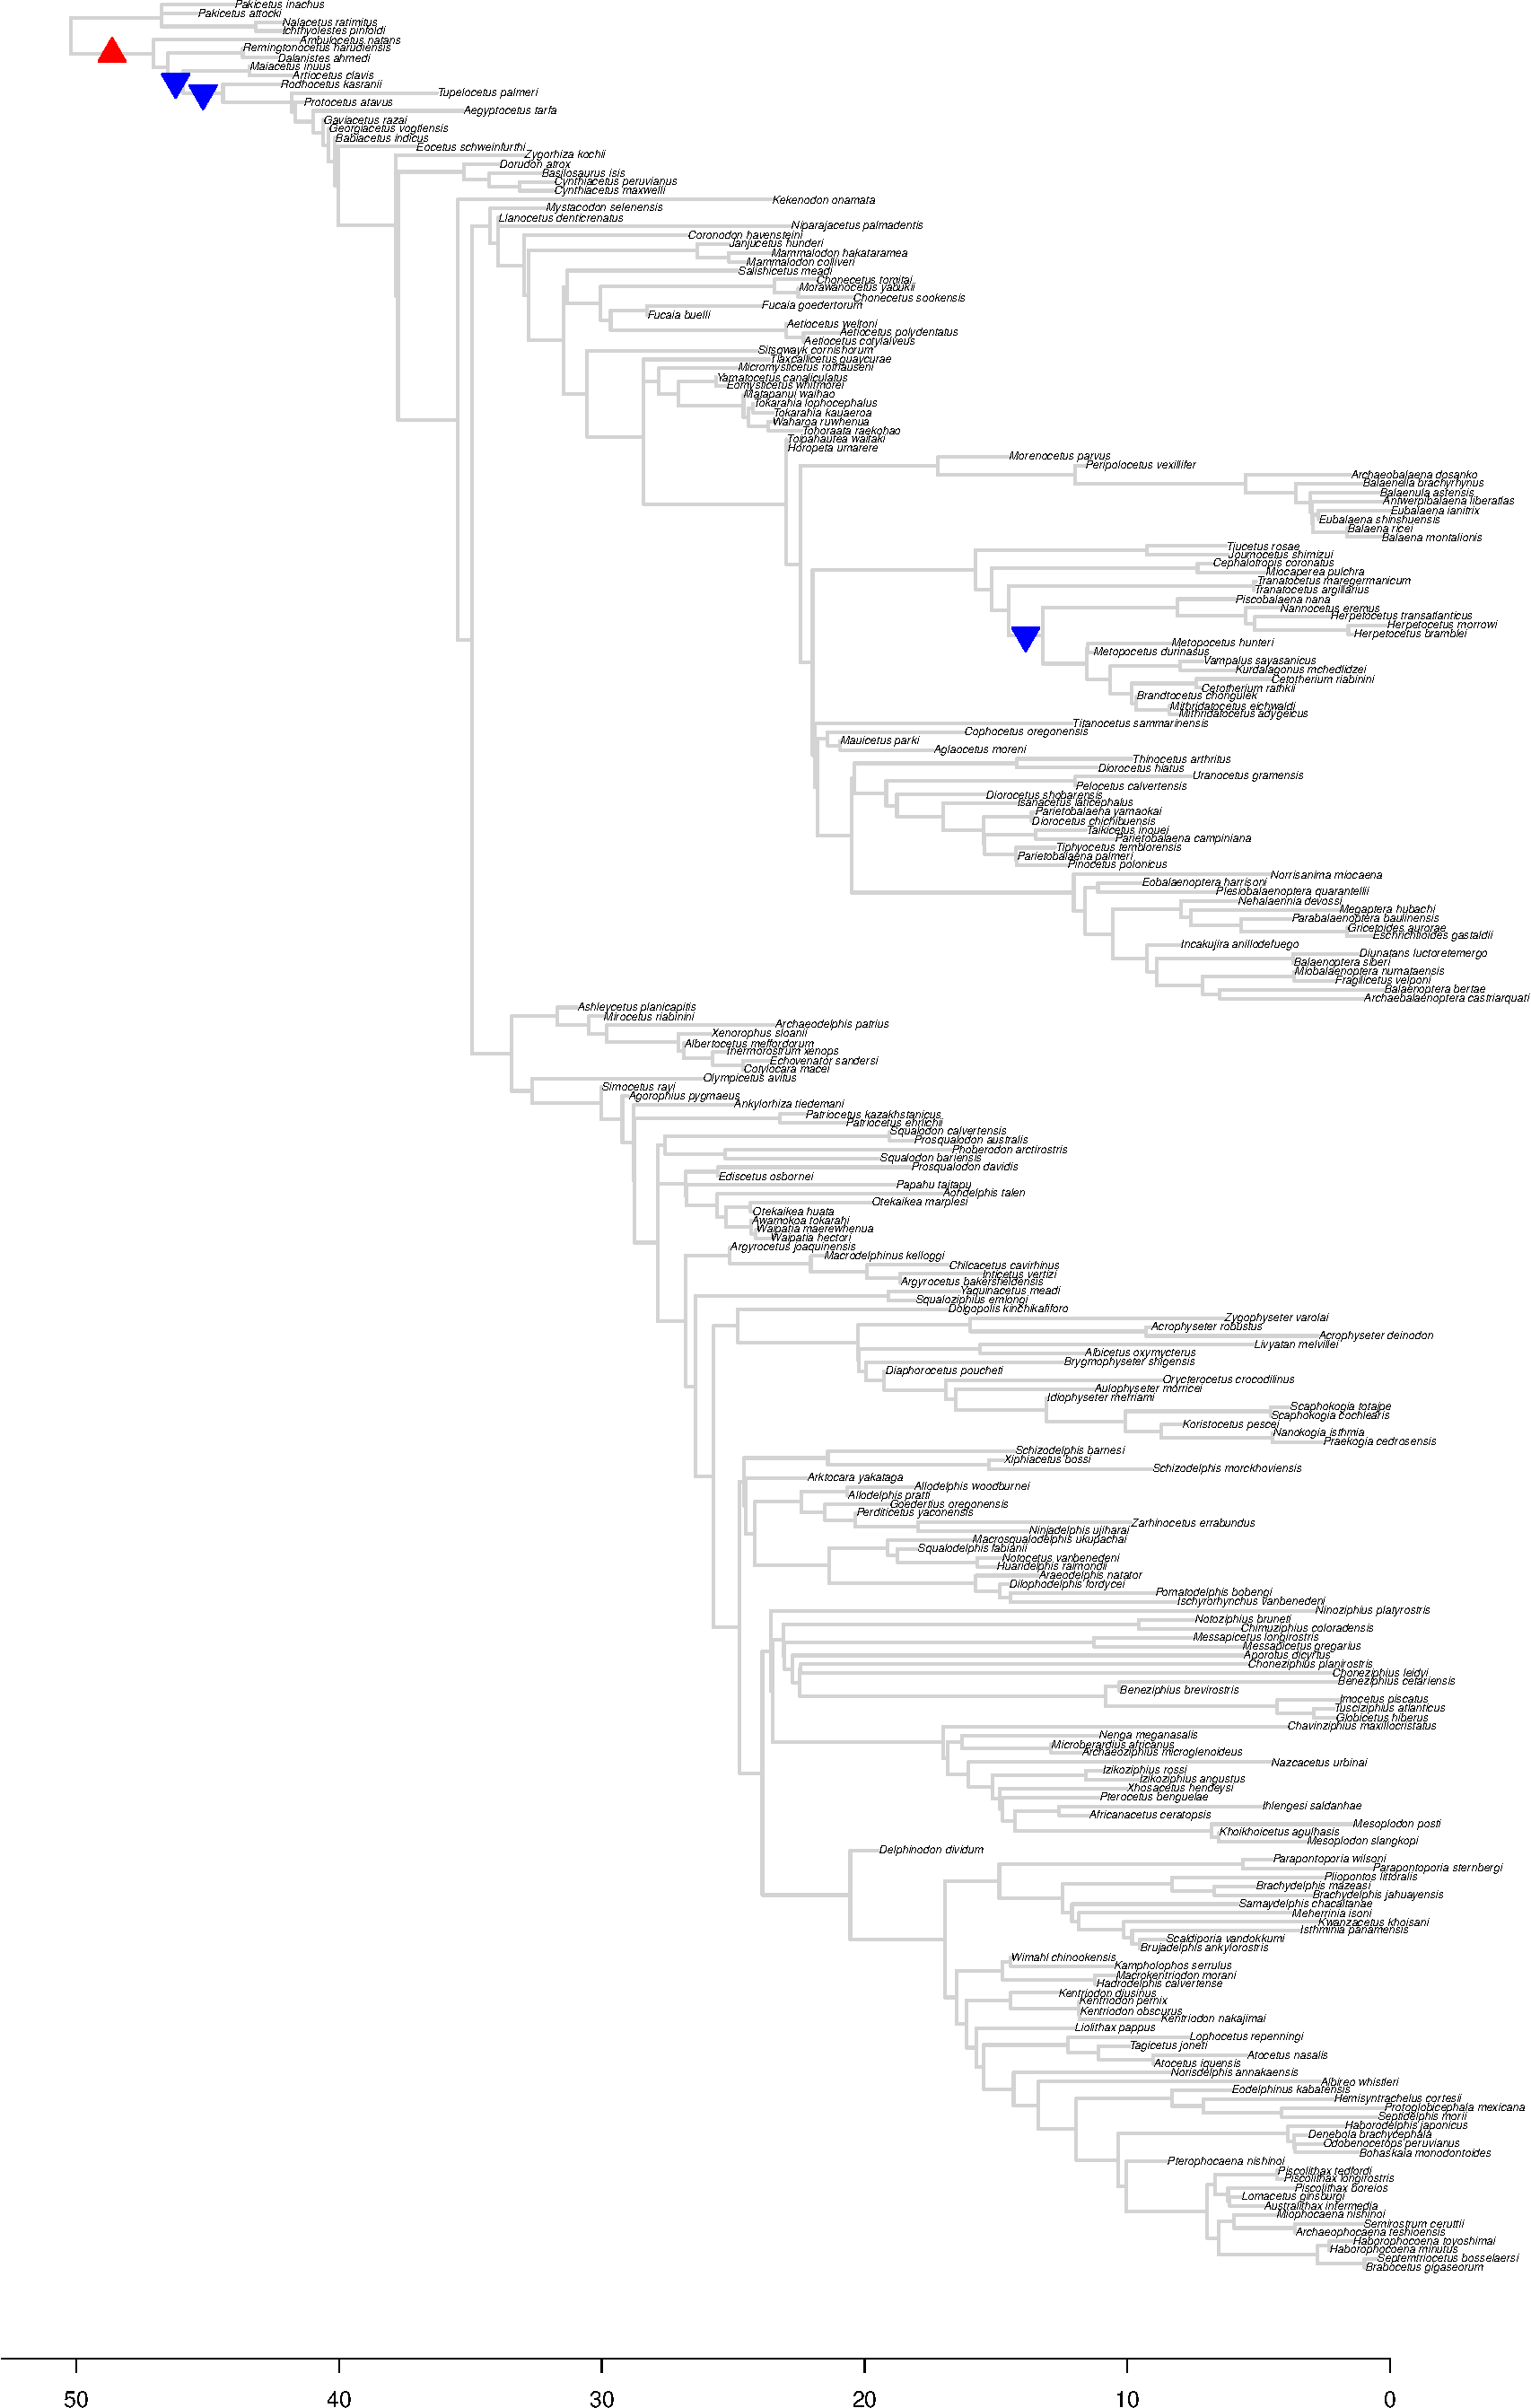
\includegraphics[width=0.8\textwidth]{img/plots-noextant-wZBL-k5-1.pdf}
\caption{Results for \textit{bayou} fit for the \textit{No Extant} tree setting the average number of shifts in the prior distribution ($\lambda$) to 5. The triangles represent the position and direction of the shifts with posterior probability higher than 0.1, with upward triangles (in red) indicating increases in $\theta$, and downward triangles (in blue) indicating decreases in $\theta$.}
\label{fig:noextant-k5}
\end{figure}

\newpage

\begin{figure}[H]
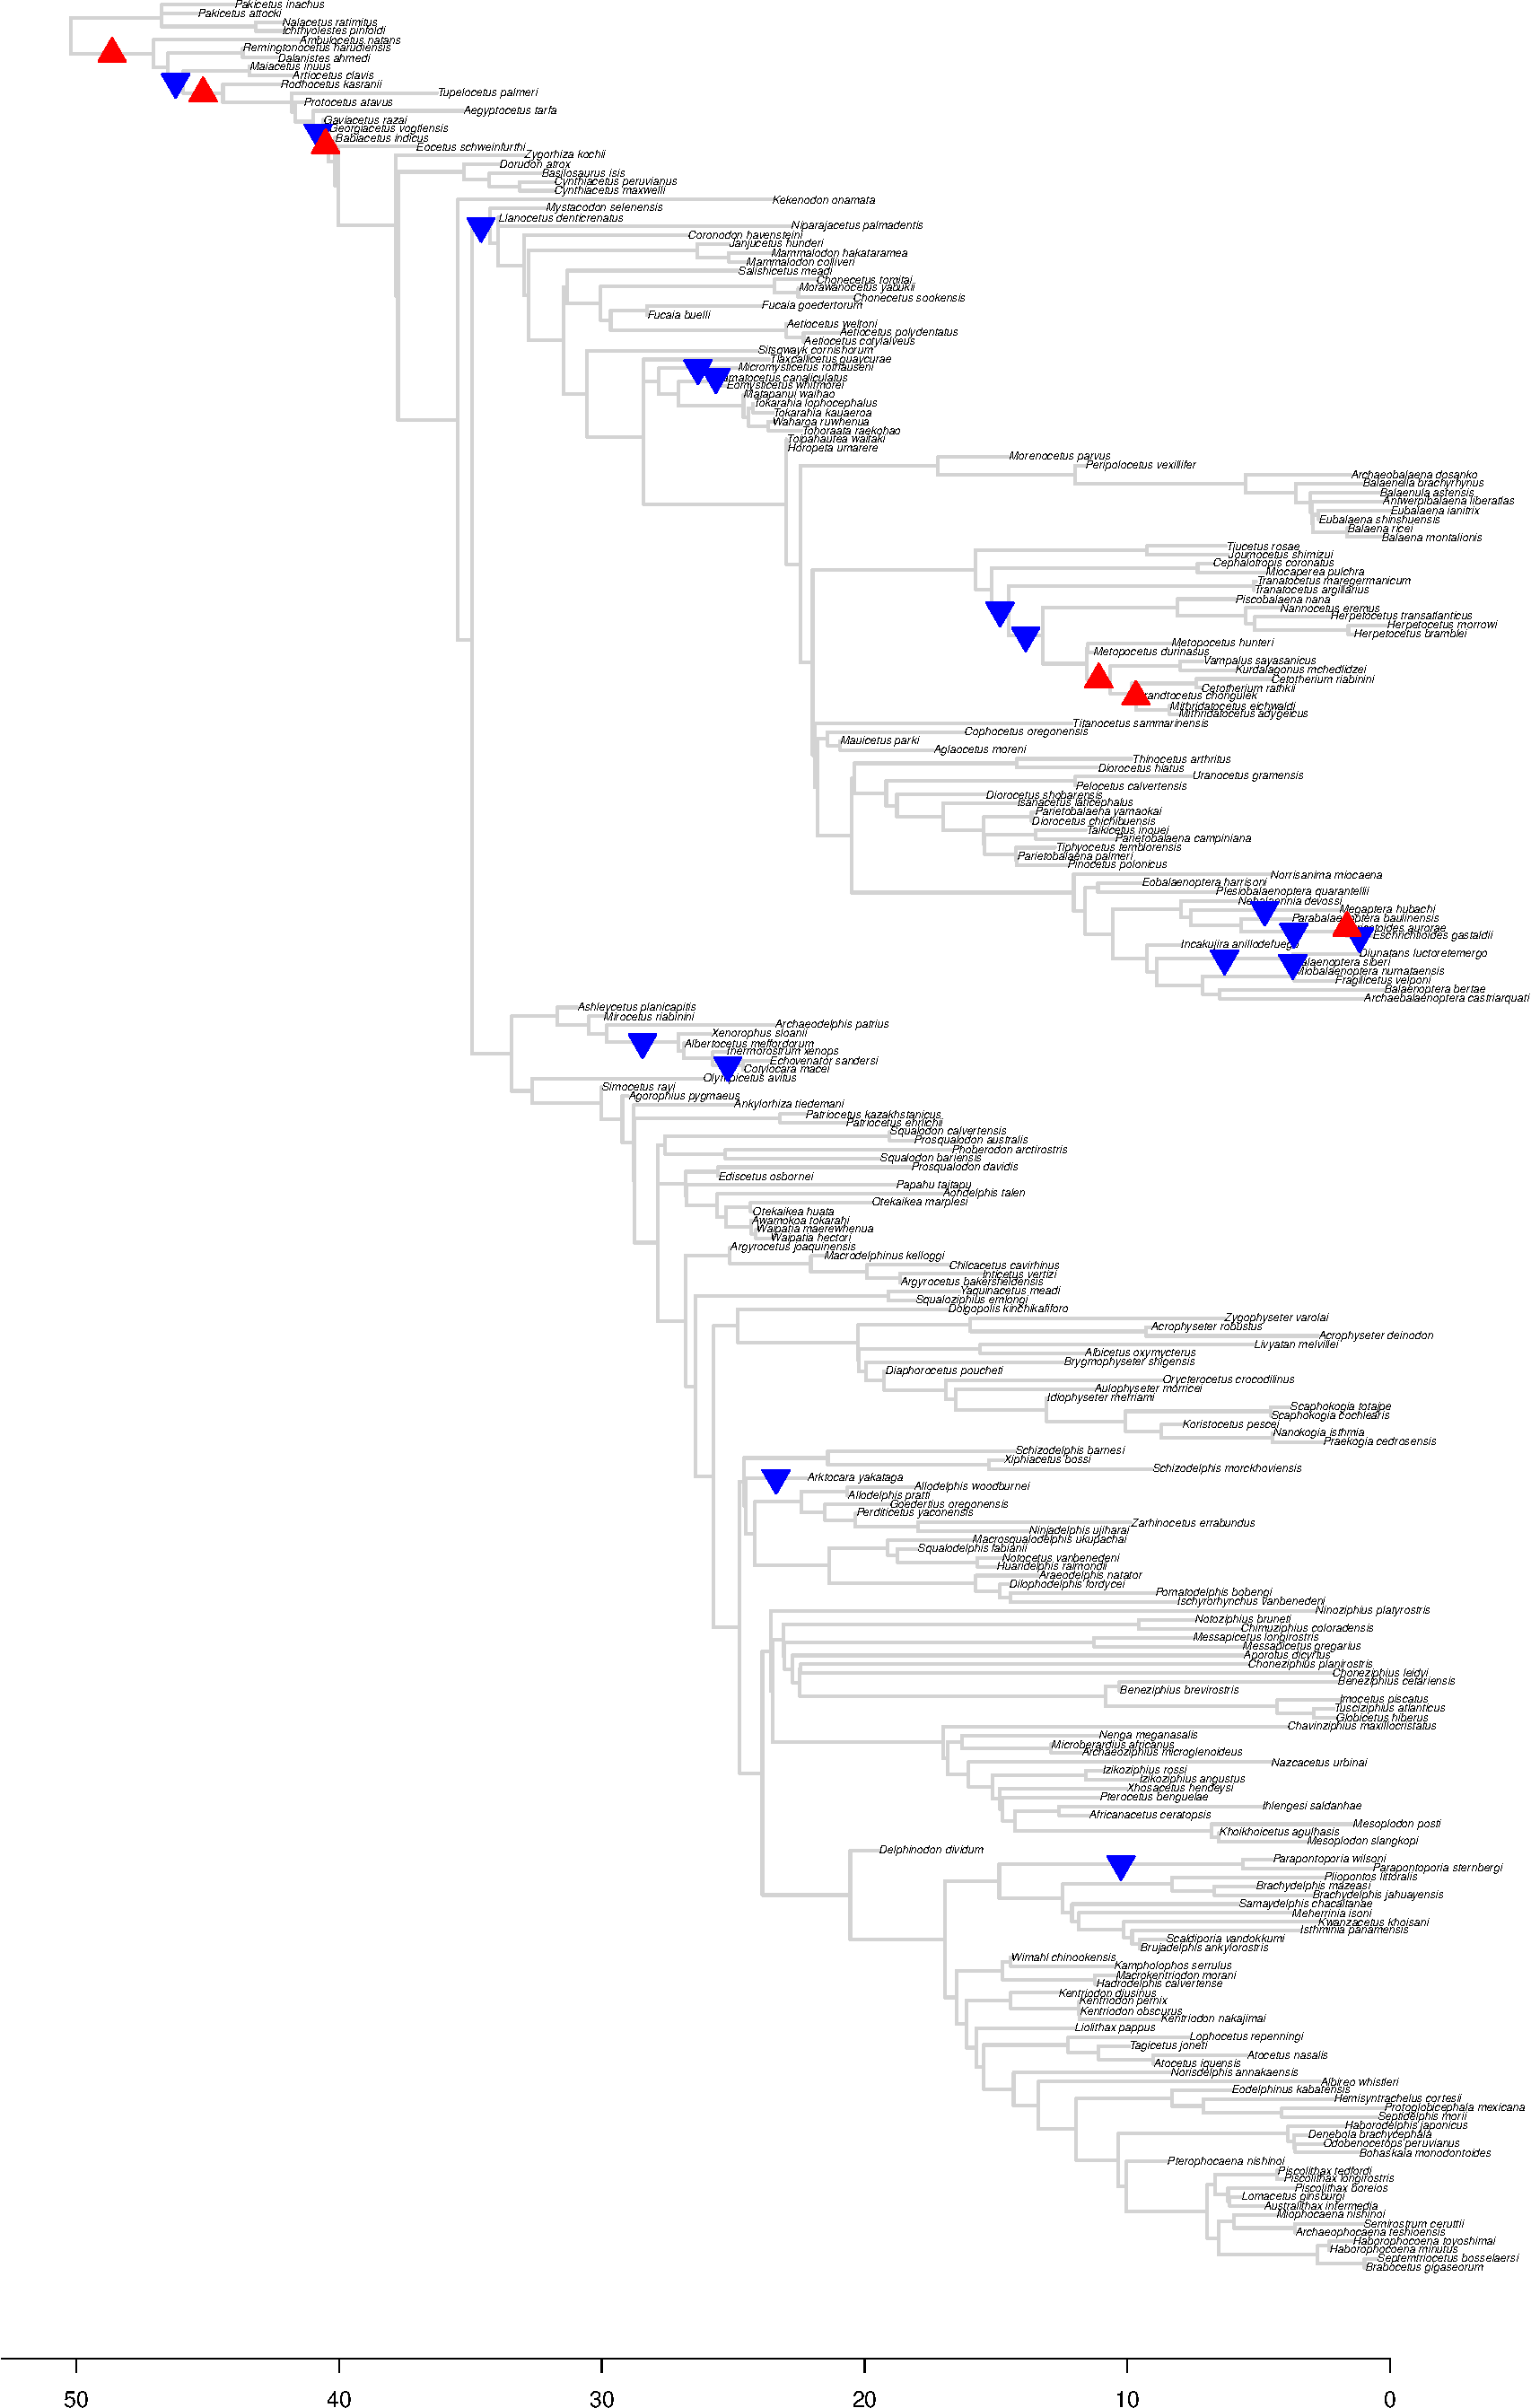
\includegraphics[width=0.9\textwidth]{img/plots-noextant-wZBL-k15-1.pdf}
\caption{Results for \textit{bayou} fit for the \textit{No Extant} tree setting the average number of shifts in the prior distribution ($\lambda$) to 15. The triangles represent the position and direction of the shifts with posterior probability higher than 0.1, with upward triangles (in red) indicating increases in $\theta$, and downward triangles (in blue) indicating decreases in $\theta$.}
\label{fig:noextant-k15}
\end{figure}

\newpage

\begin{figure}[H]
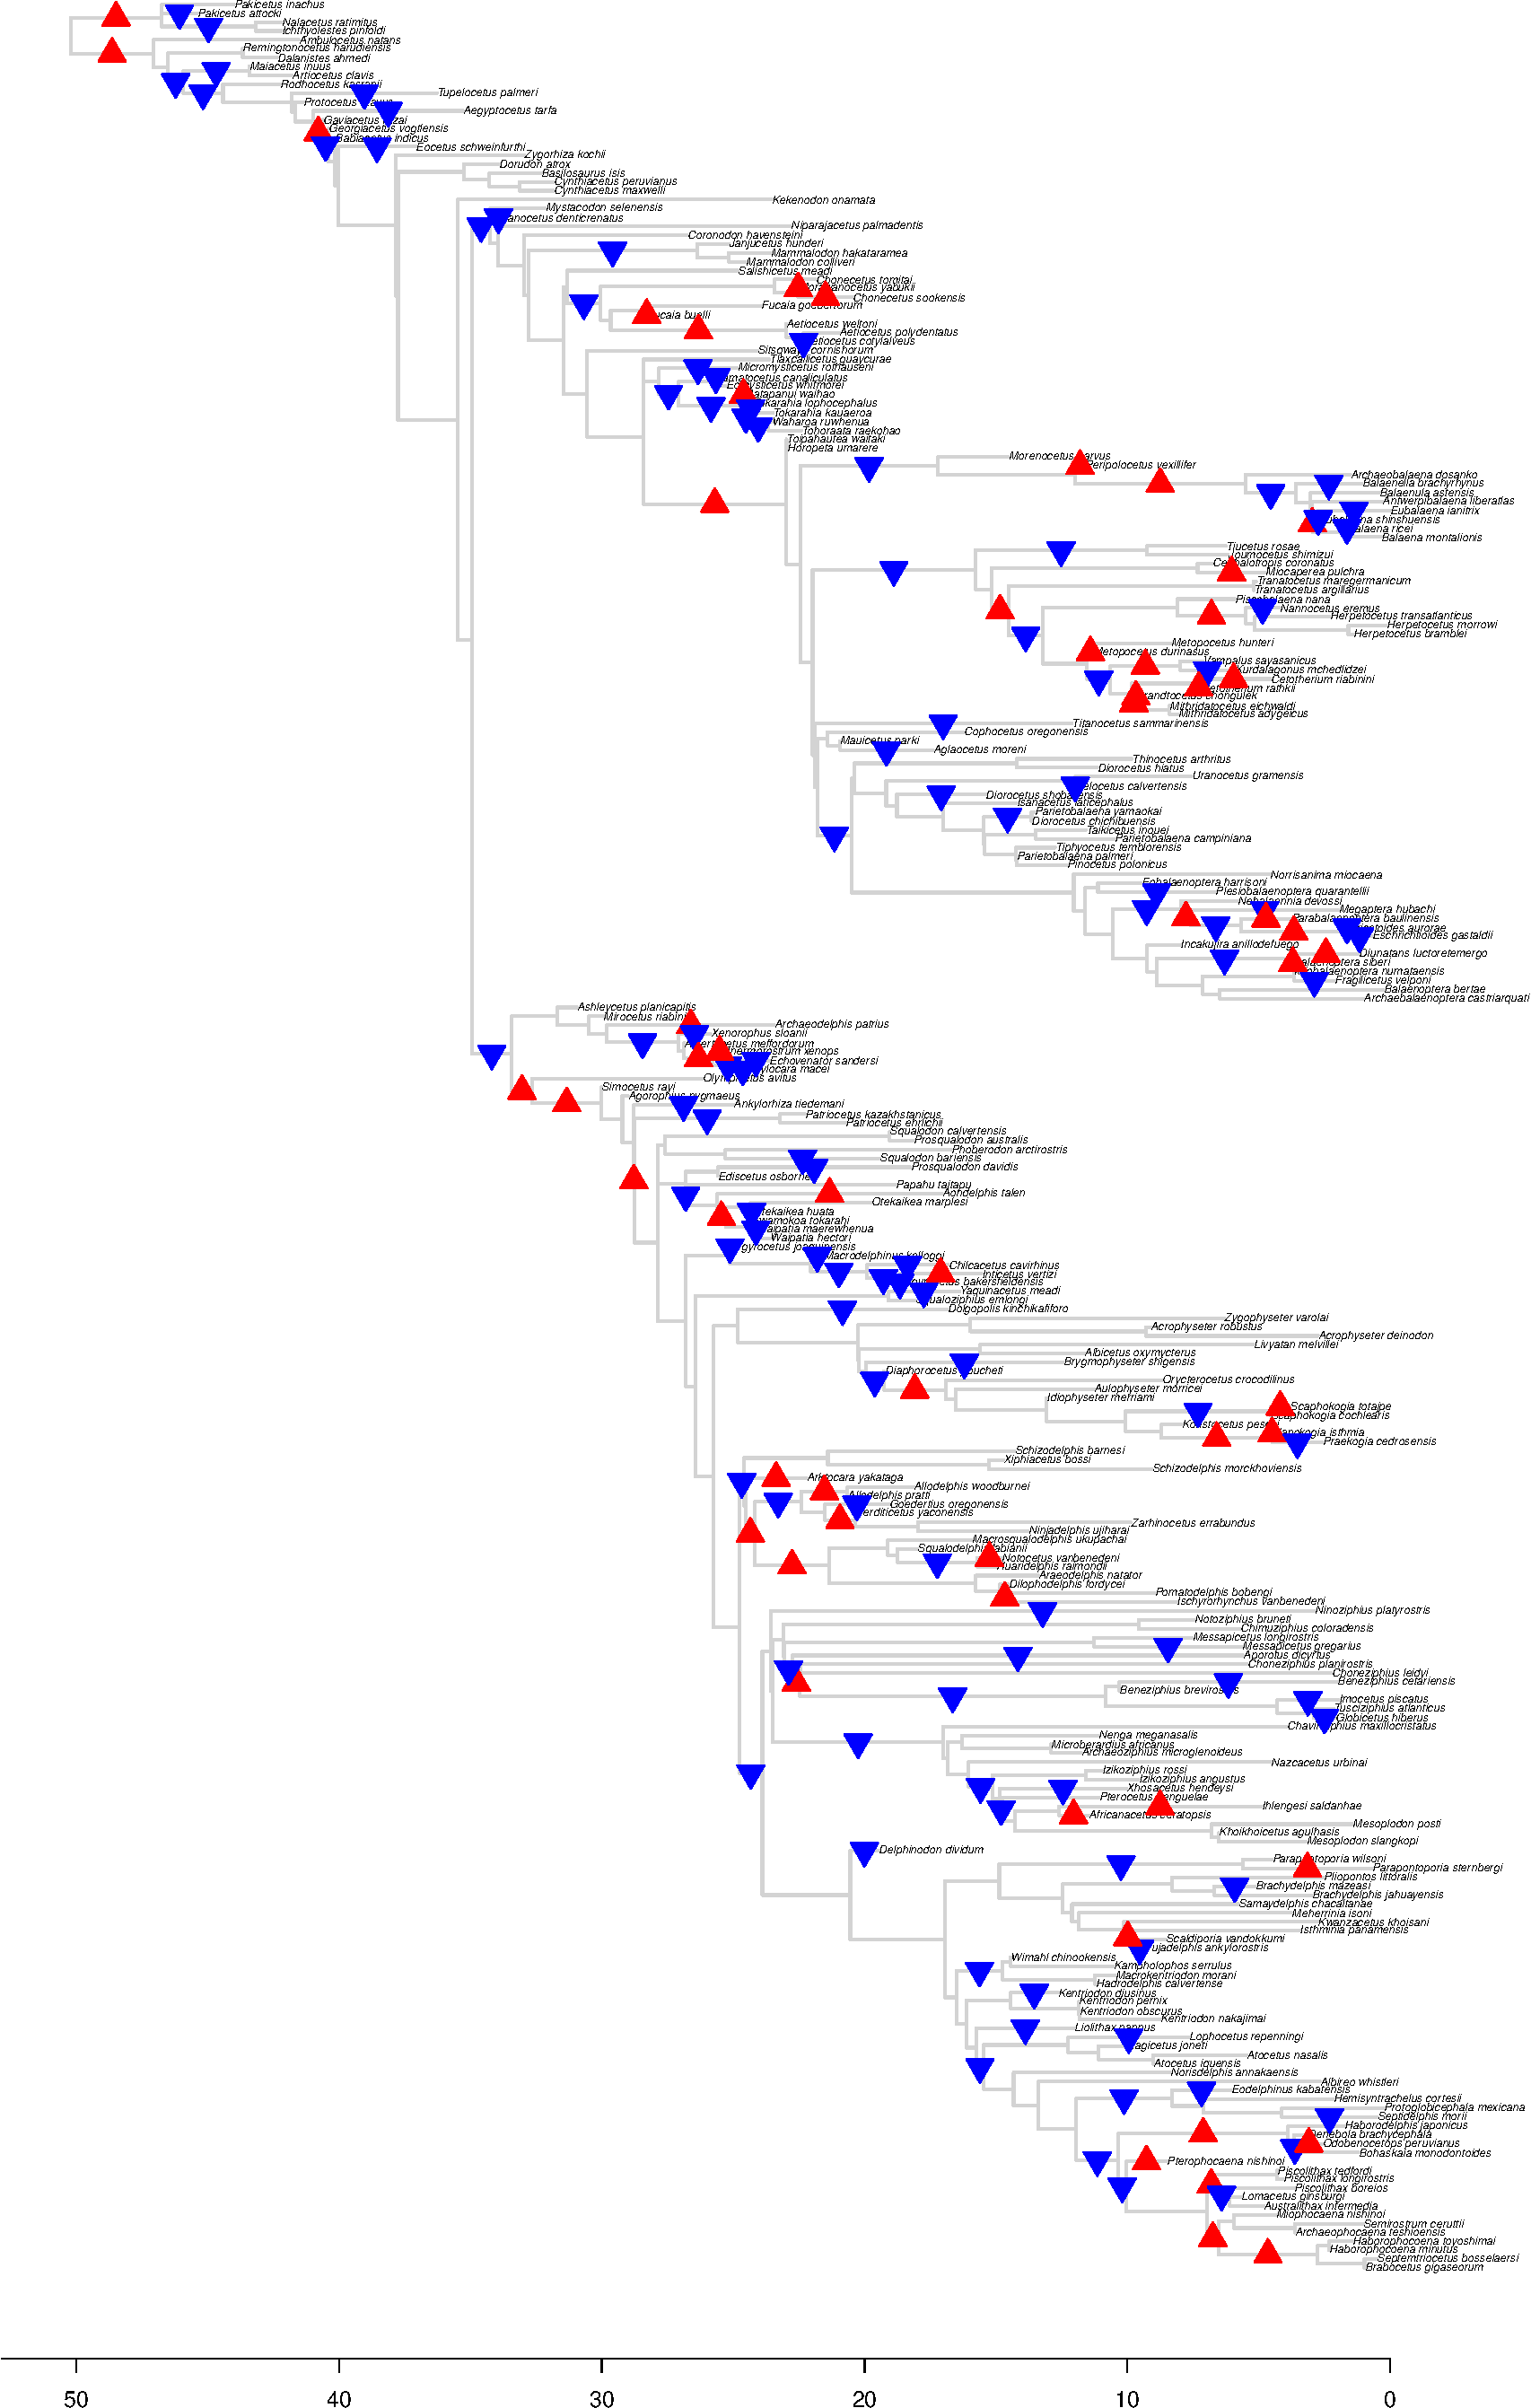
\includegraphics[width=0.9\textwidth]{img/plots-noextant-wZBL-k50-1.pdf}
\caption{Results for \textit{bayou} fit for the \textit{No Extant} tree setting the average number of shifts in the prior distribution ($\lambda$) to 50. The triangles represent the position and direction of the shifts with posterior probability higher than 0.1, with upward triangles (in red) indicating increases in $\theta$, and downward triangles (in blue) indicating decreases in $\theta$.}
\label{fig:noextant-k50}
\end{figure}

\newpage

\begin{figure}[H]
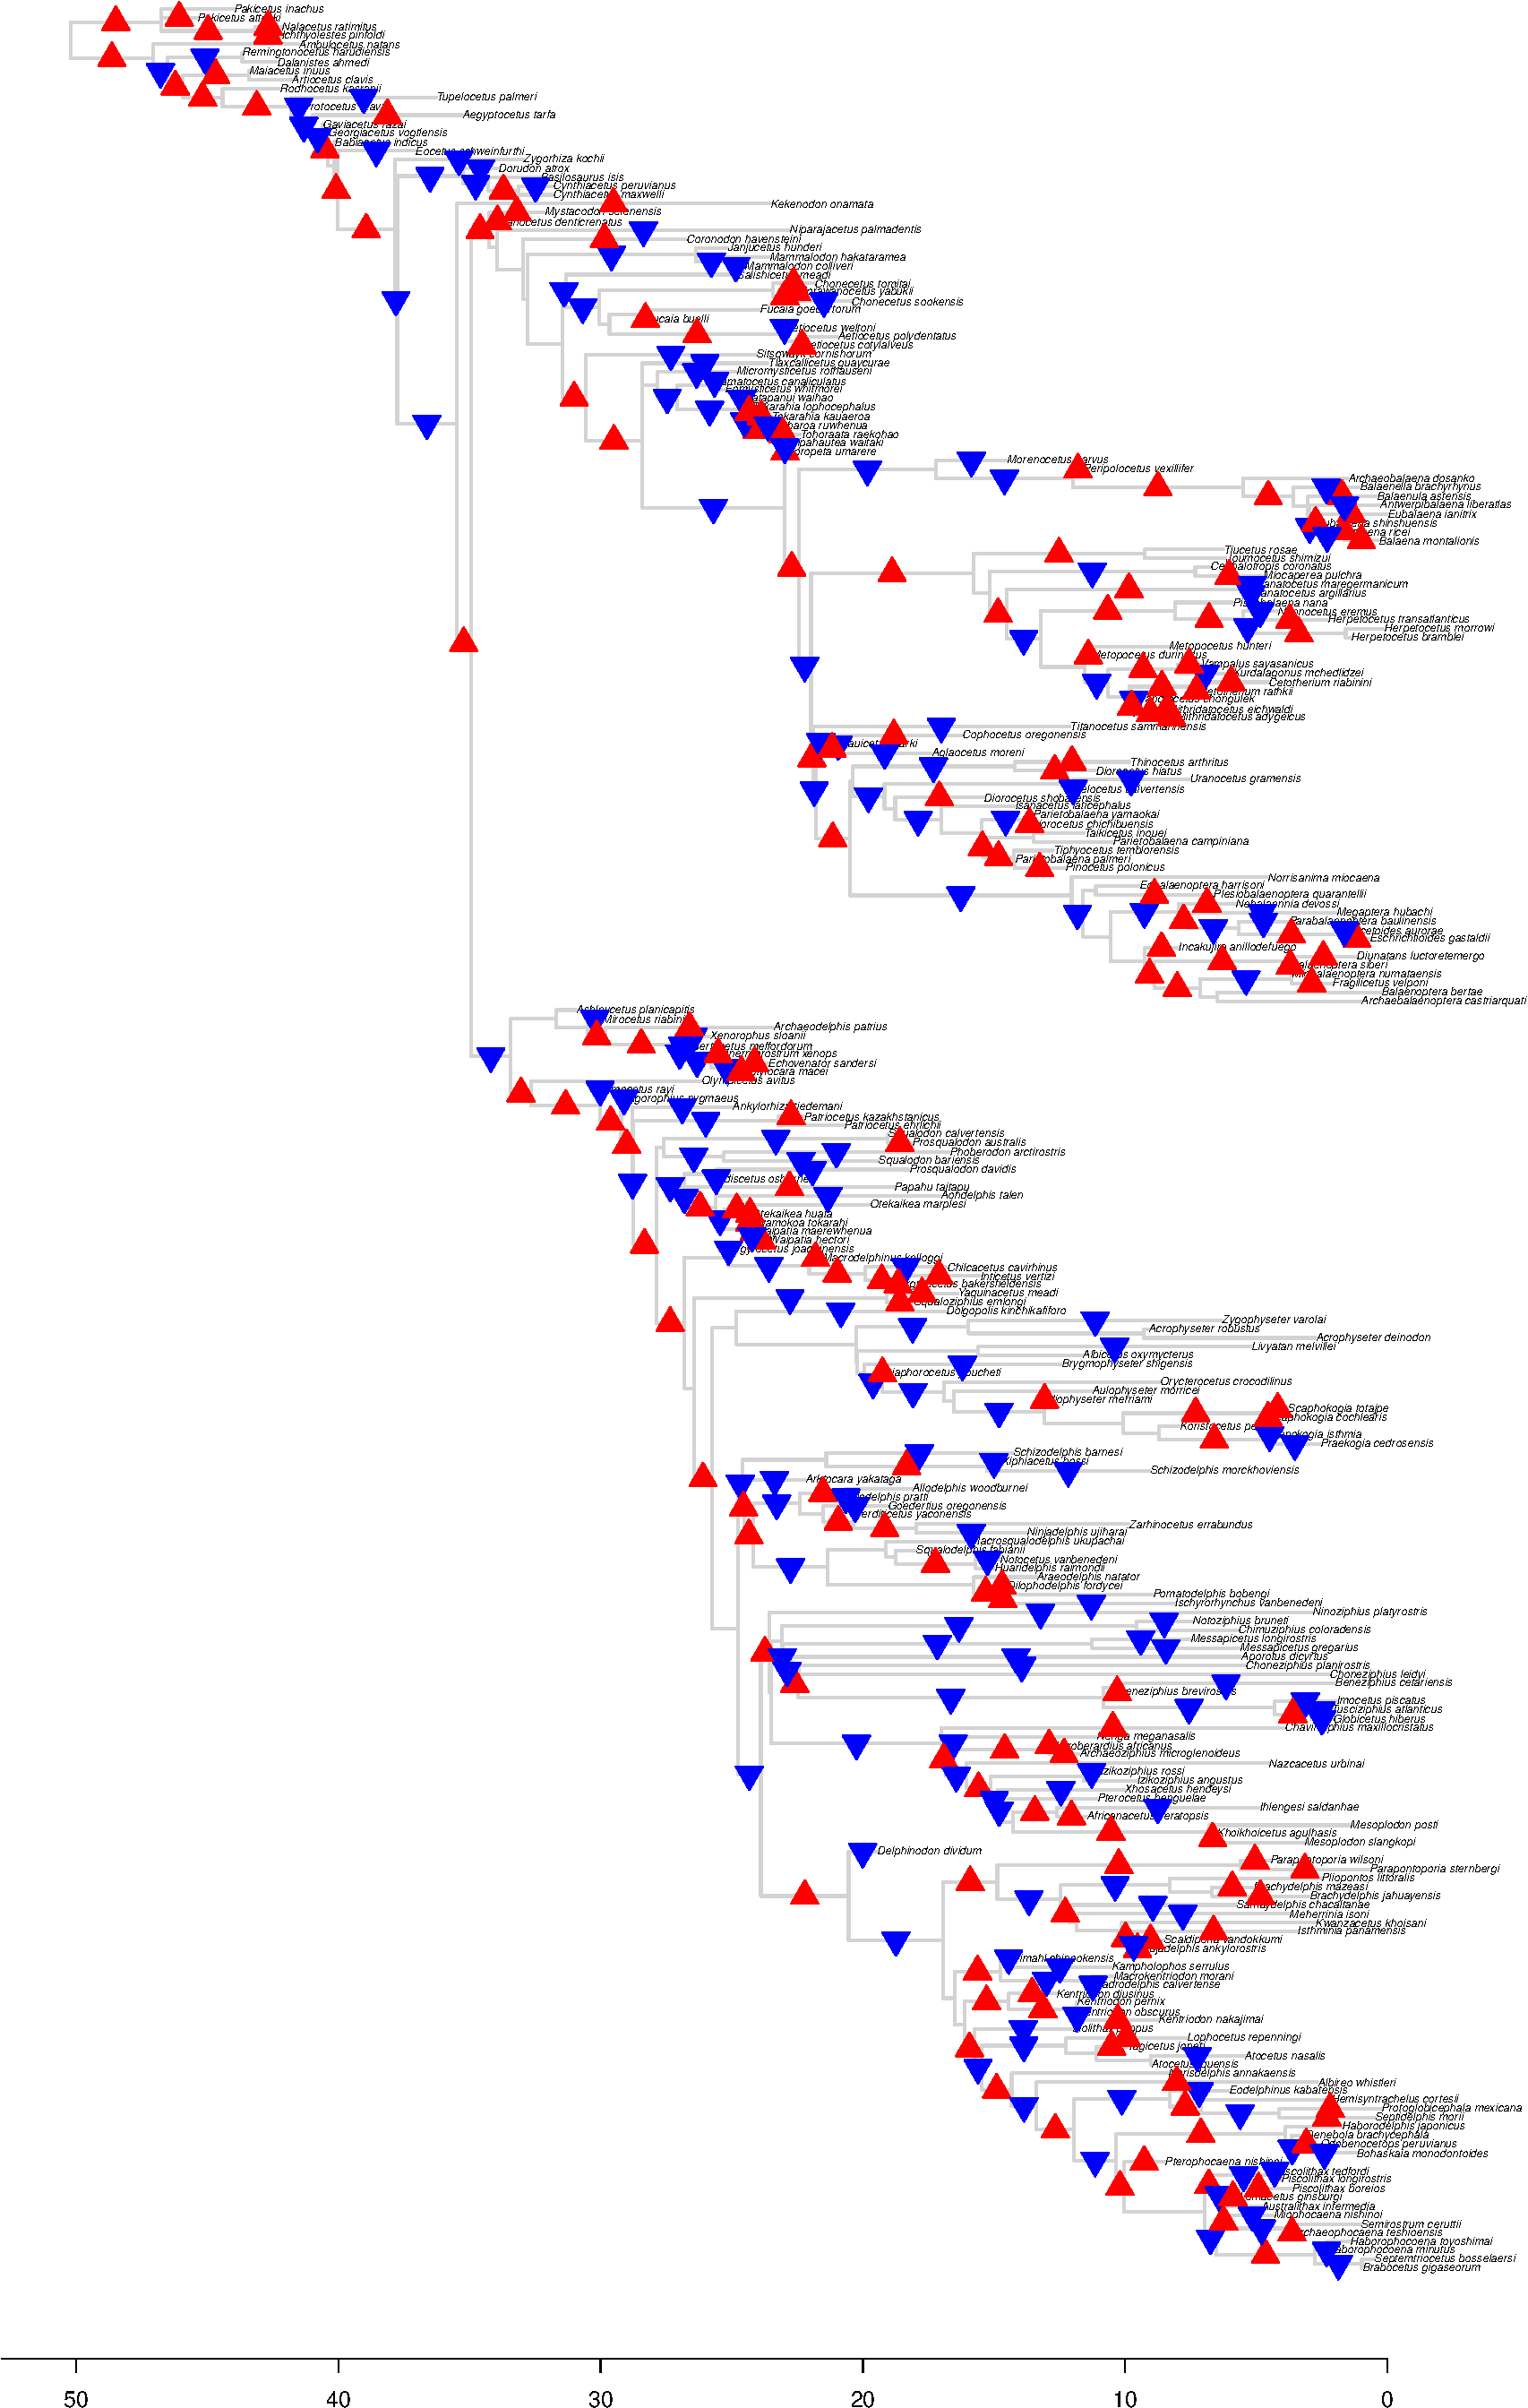
\includegraphics[width=0.9\textwidth]{img/plots-noextant-wZBL-k250-1.pdf}
\caption{Results for \textit{bayou} fit for the \textit{No Extant} tree setting the average number of shifts in the prior distribution ($\lambda$) to 250. The triangles represent the position and direction of the shifts with posterior probability higher than 0.1, with upward triangles (in red) indicating increases in $\theta$, and downward triangles (in blue) indicating decreases in $\theta$.}
\label{fig:noextant-k250}
\end{figure}

\newpage

\begin{figure}[H]
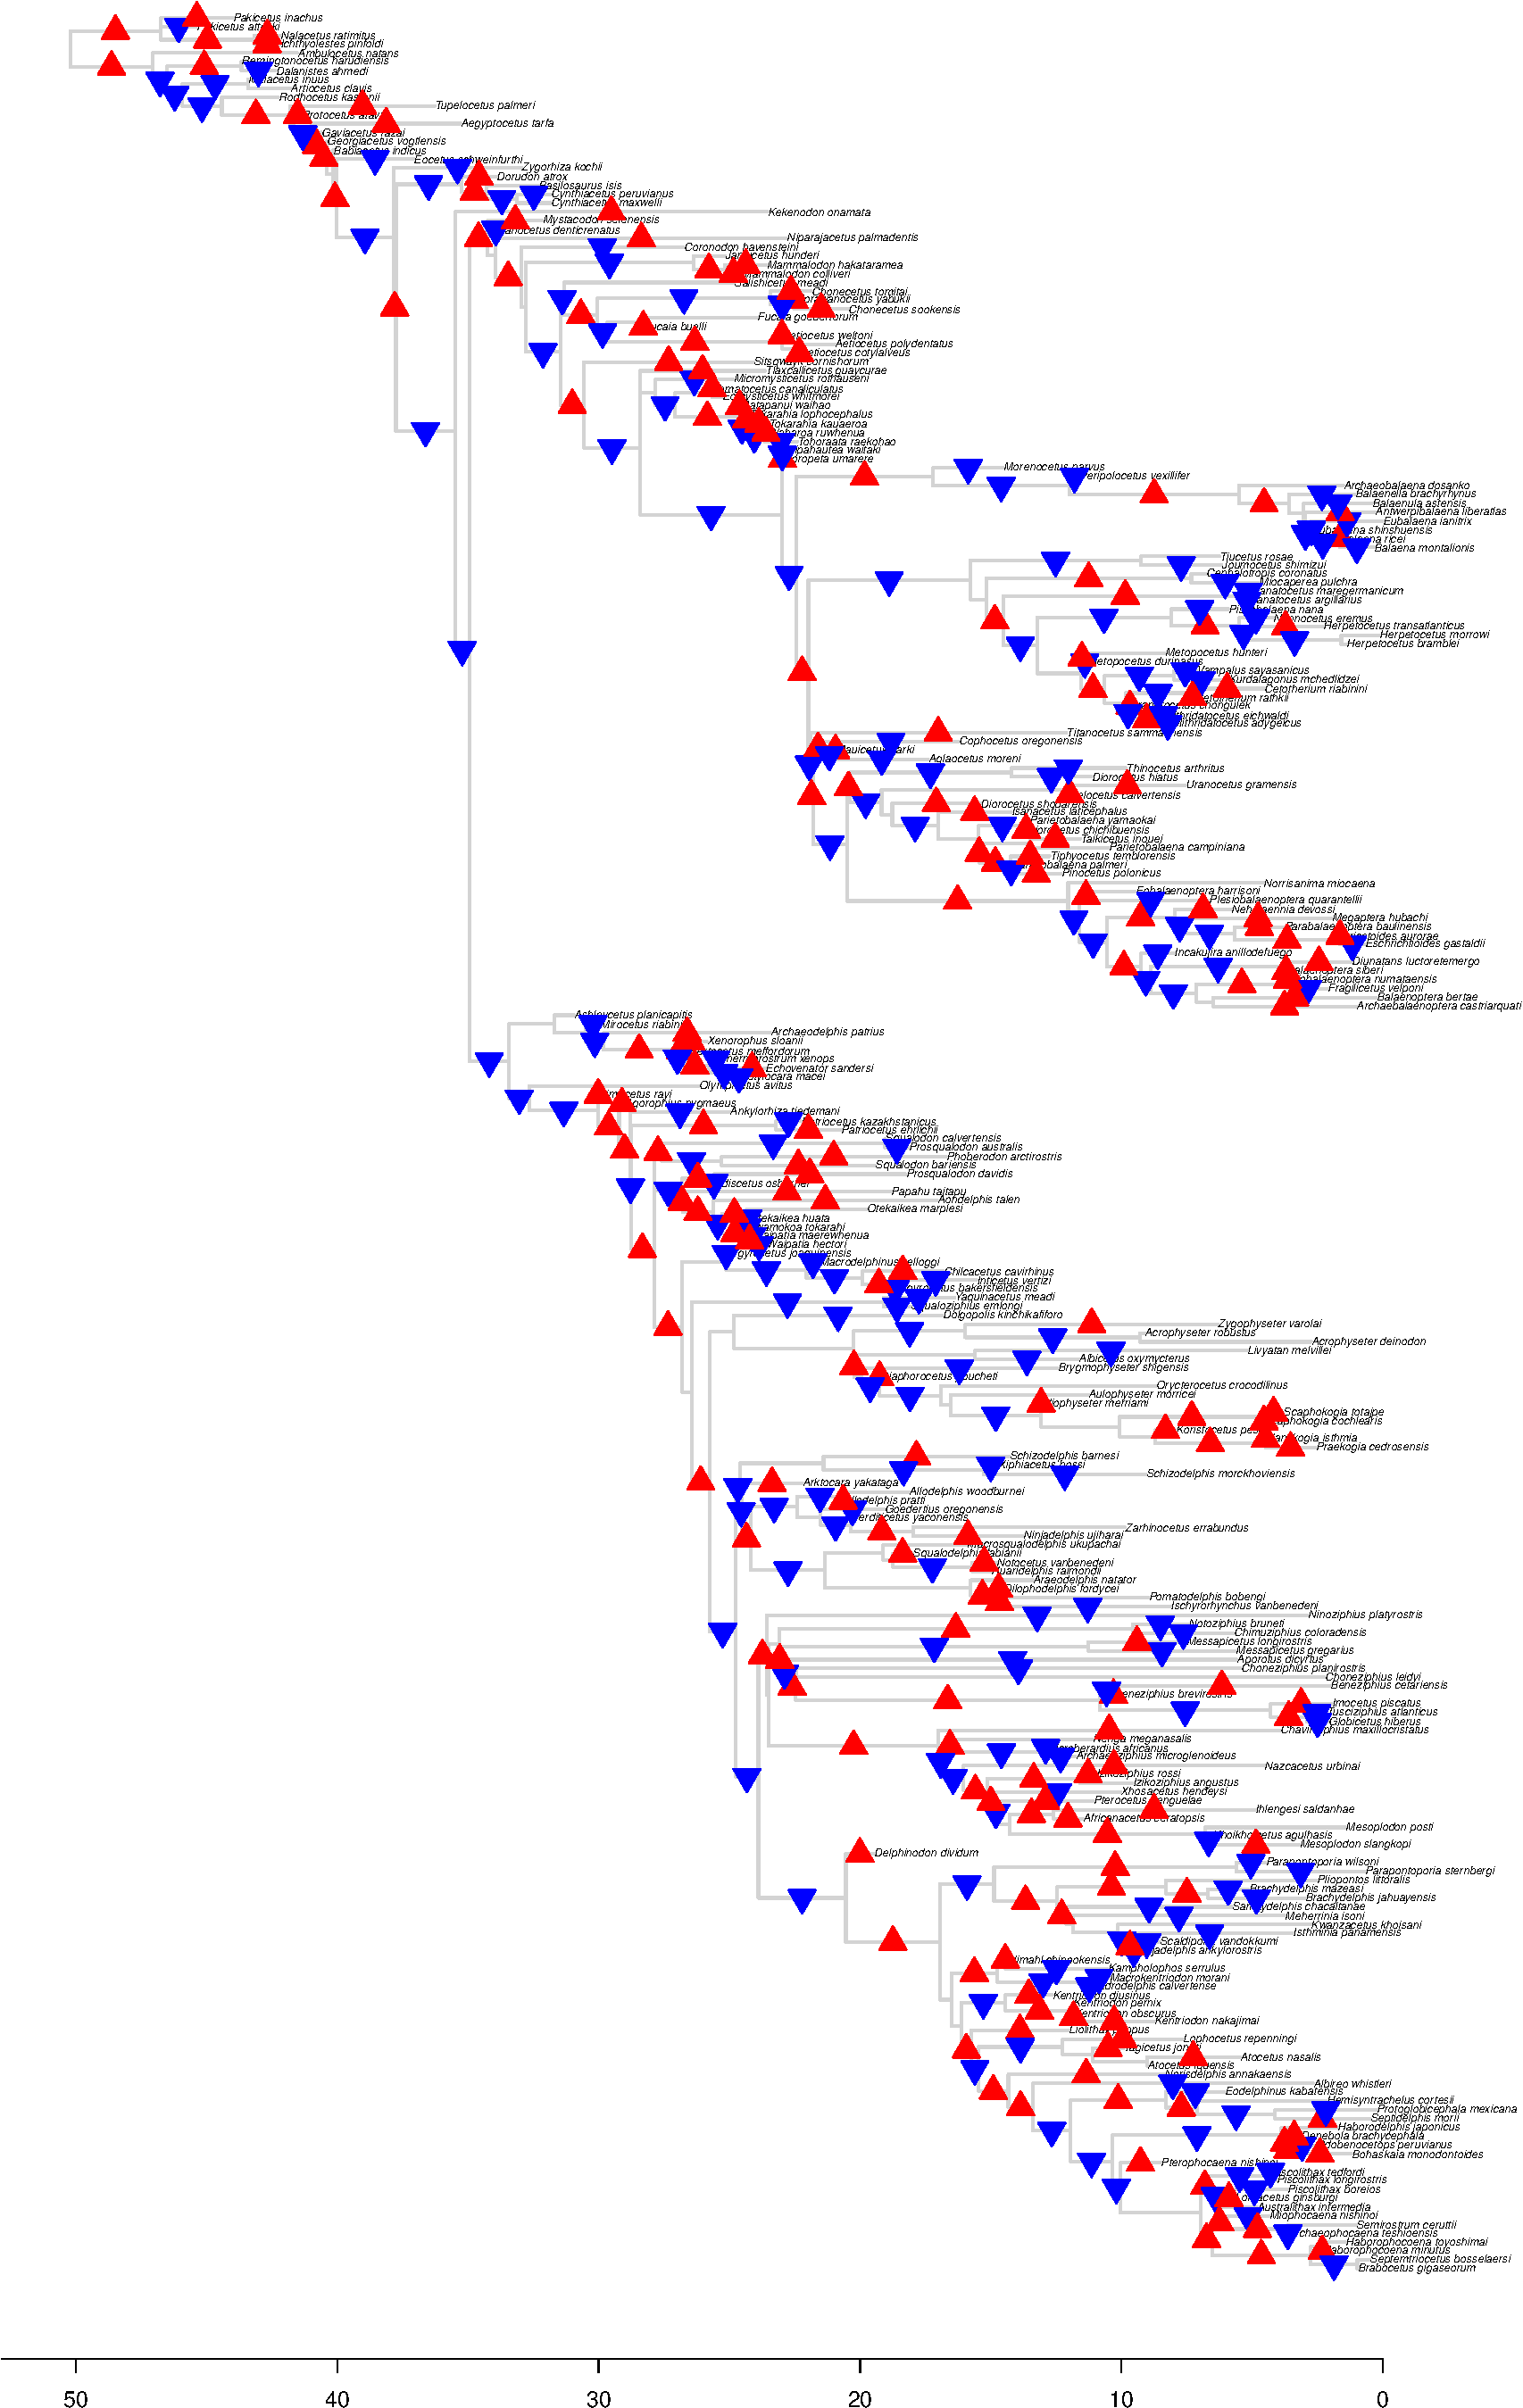
\includegraphics[width=0.9\textwidth]{img/plots-noextant-wZBL-k500-1.pdf}
\caption{Results for \textit{bayou} fit for the \textit{No Extant} tree setting the average number of shifts in the prior distribution ($\lambda$) to 500. The triangles represent the position and direction of the shifts with posterior probability higher than 0.1, with upward triangles (in red) indicating increases in $\theta$, and downward triangles (in blue) indicating decreases in $\theta$.}
\label{fig:noextant-k500}
\end{figure}

%---------------------------------------------------------------------
\subsubsection{\textit{No Imput} tree}
%---------------------------------------------------------------------

\begin{figure}[H]
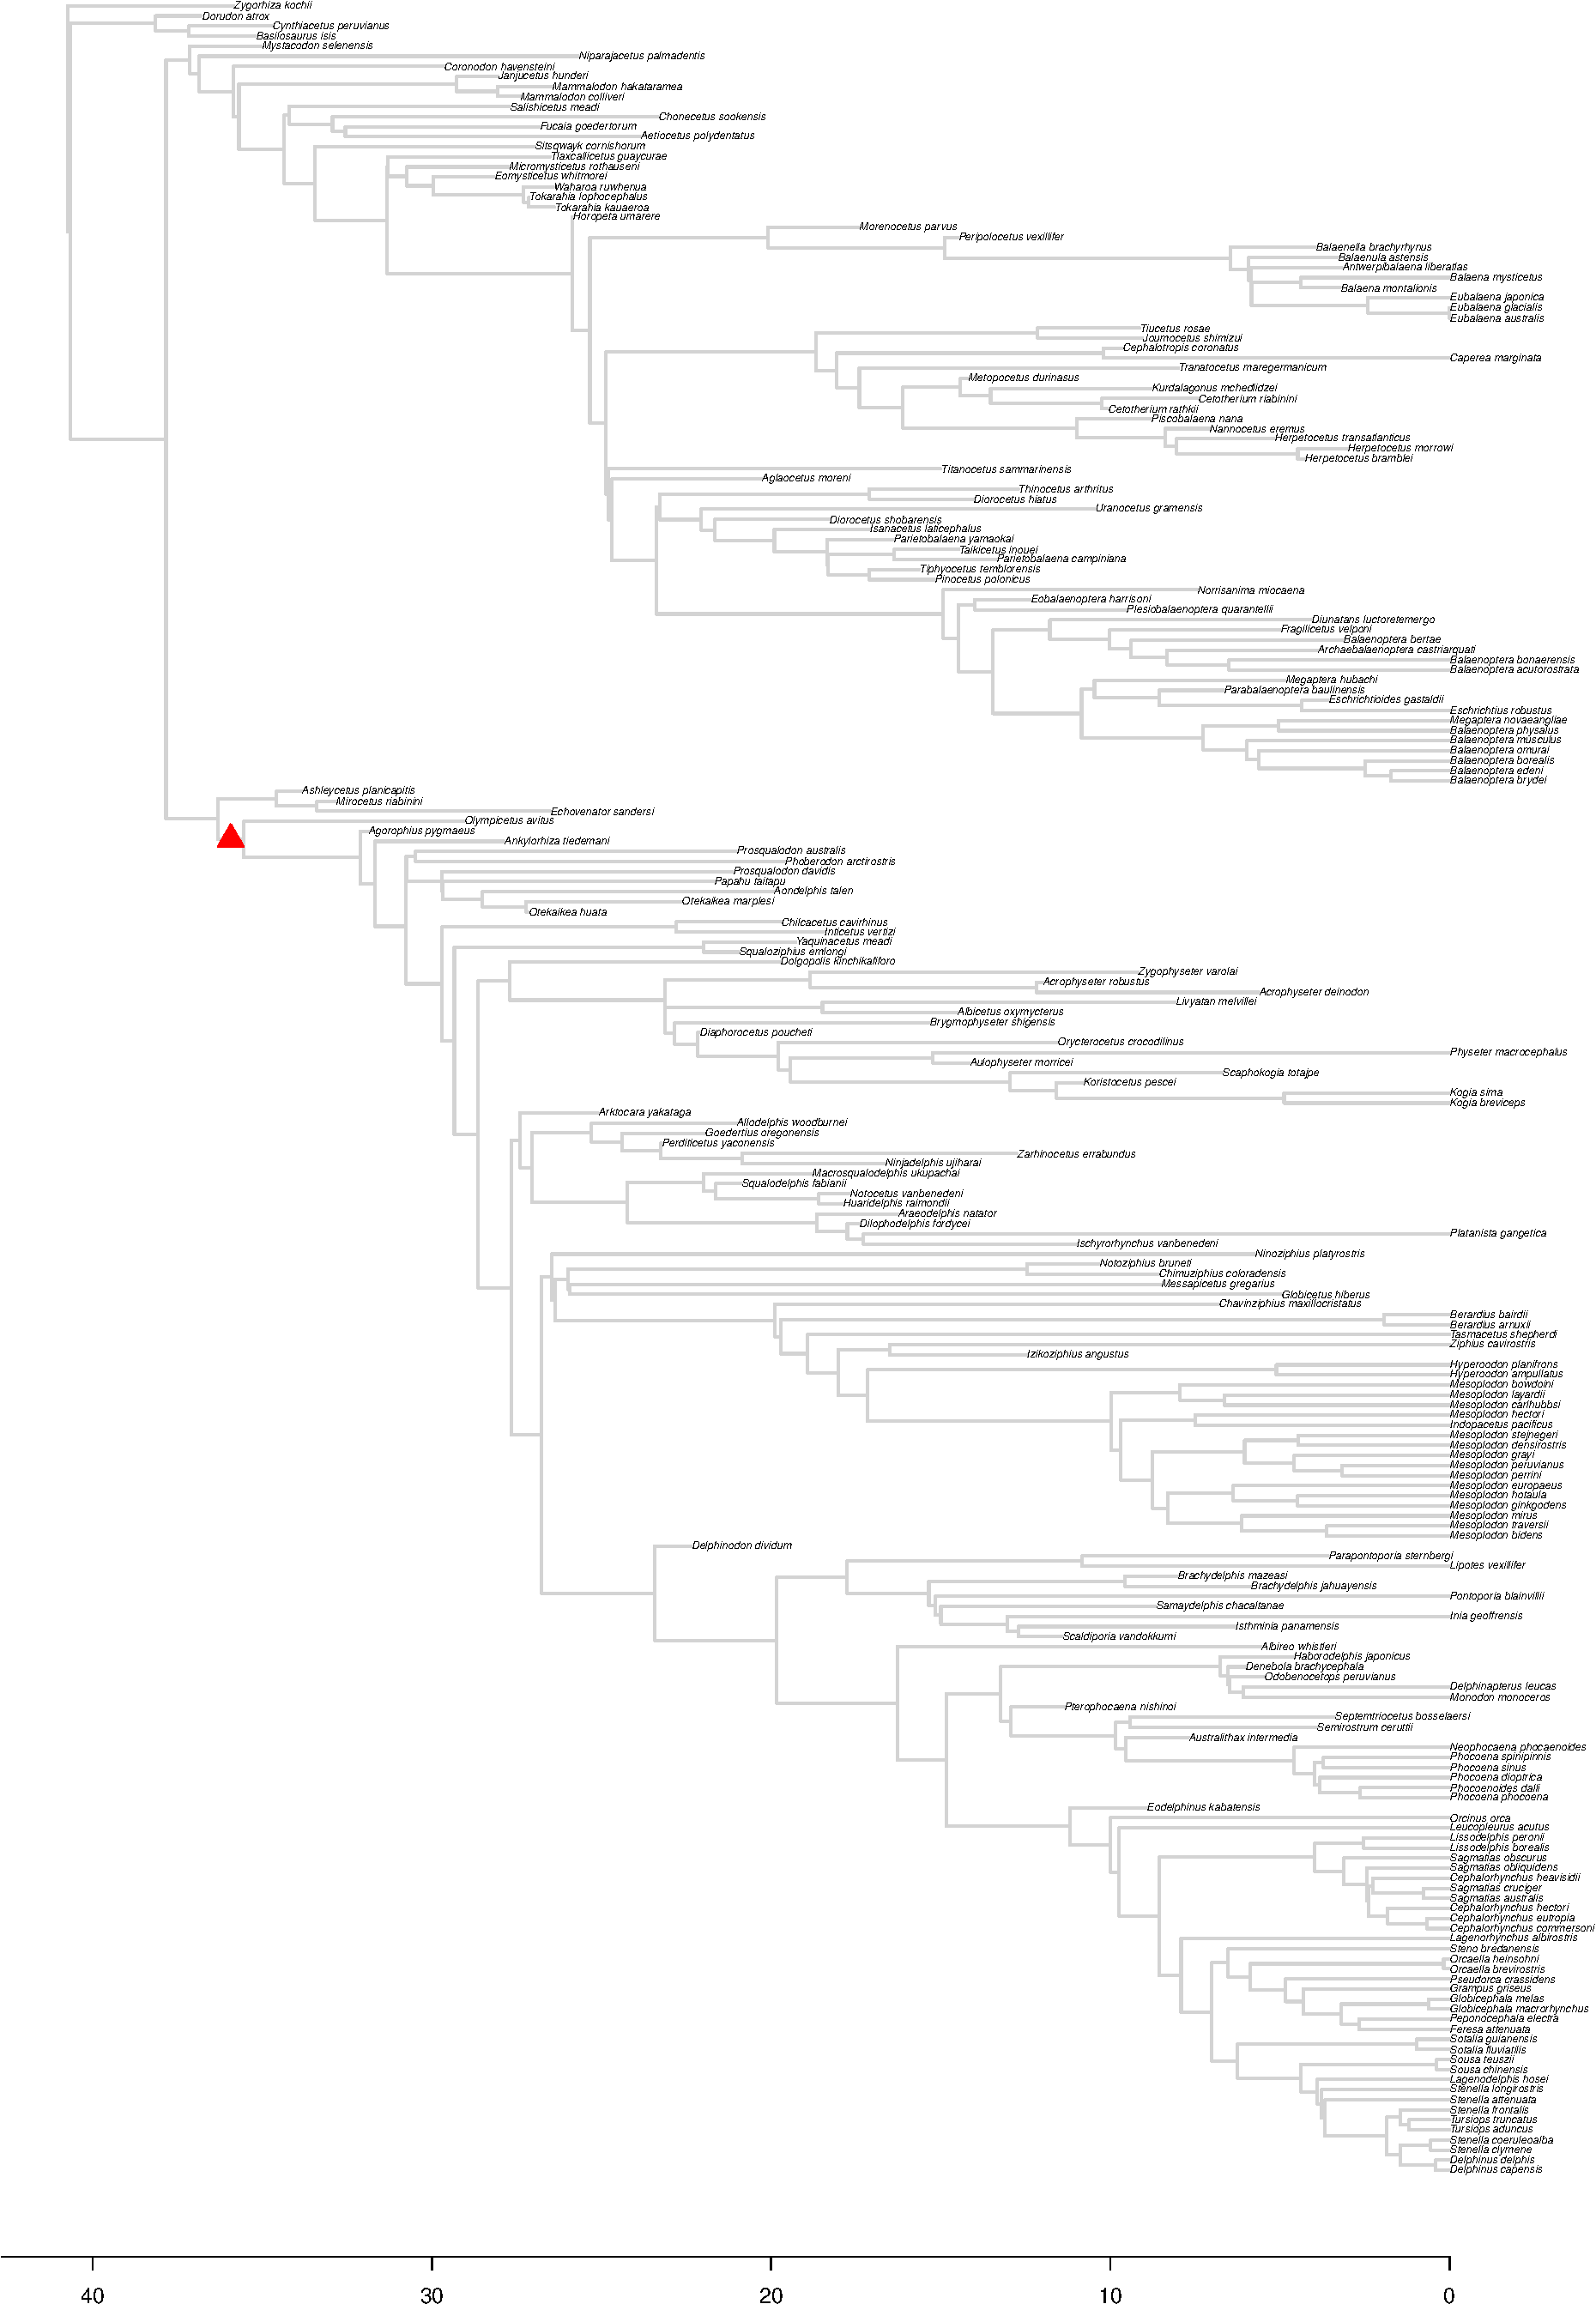
\includegraphics[width=0.8\textwidth]{img/plots-noimput-k5-1.pdf}
\caption{Results for \textit{bayou} fit for the \textit{No Imput} tree setting the average number of shifts in the prior distribution ($\lambda$) to 5. The triangles represent the position and direction of the shifts with posterior probability higher than 0.1, with upward triangles (in red) indicating increases in $\theta$, and downward triangles (in blue) indicating decreases in $\theta$.}
\label{fig:noimput-k5}
\end{figure}

\newpage

\begin{figure}[H]
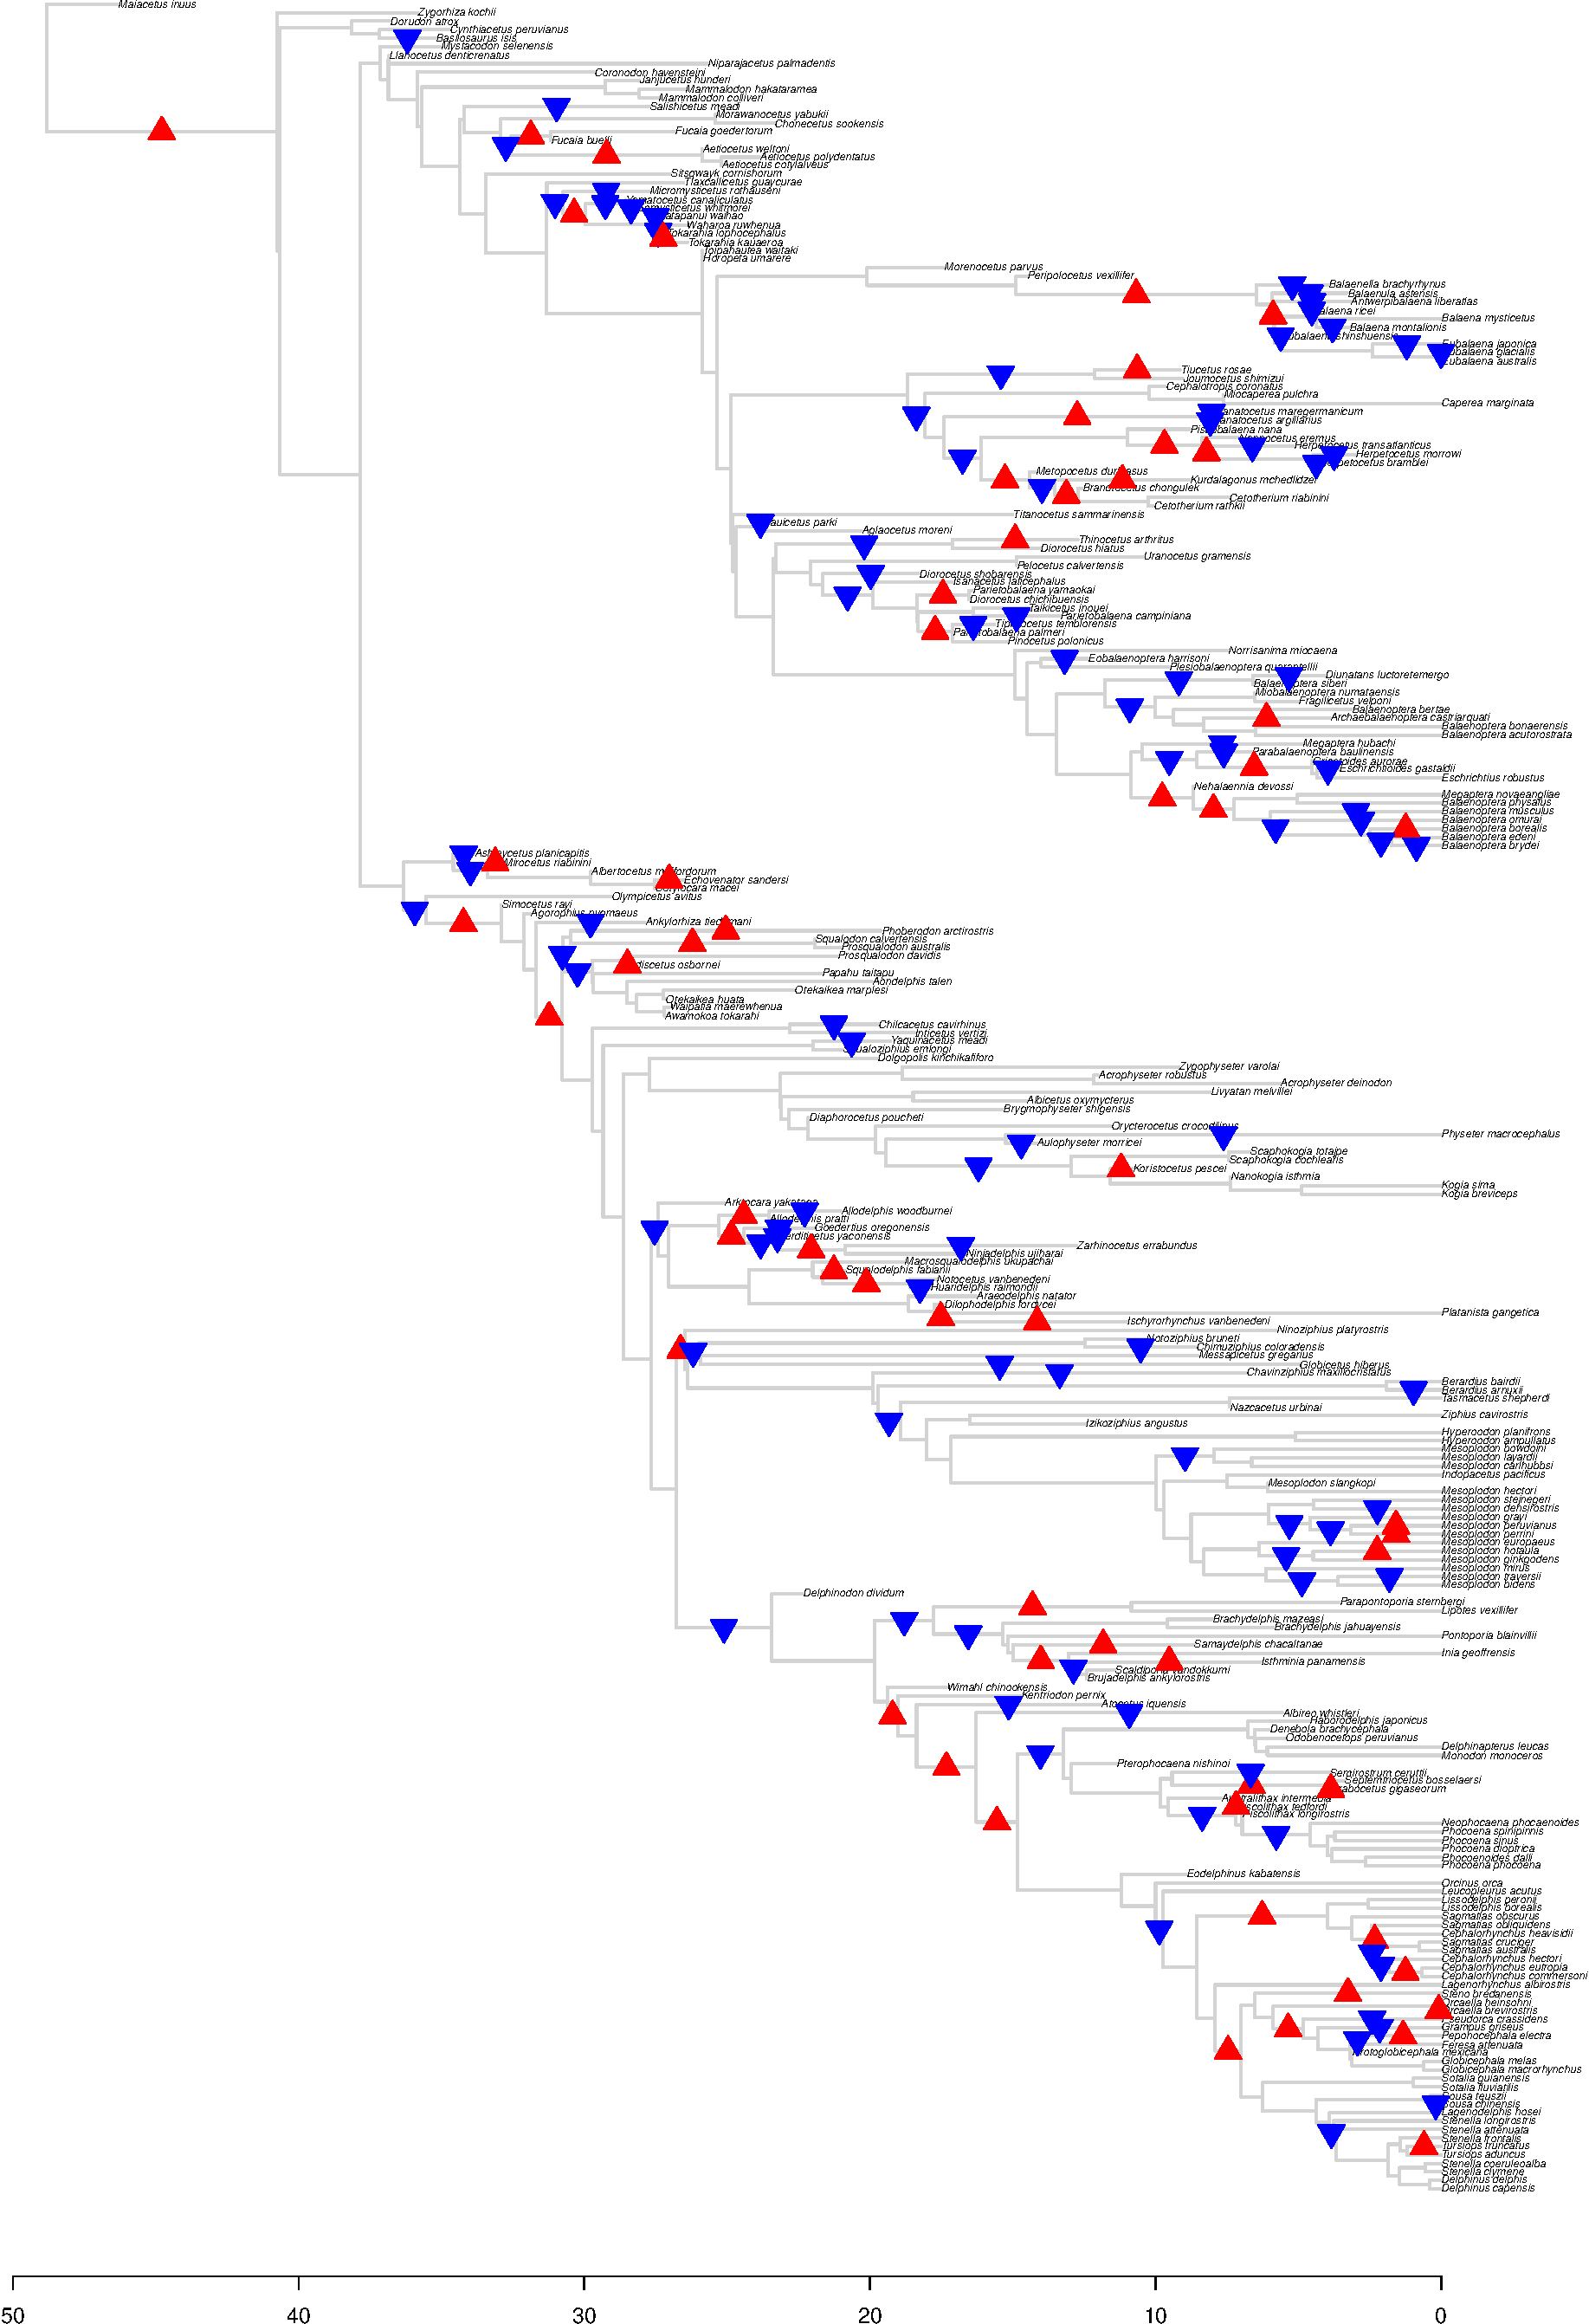
\includegraphics[width=0.9\textwidth]{img/plots-noimput-wZBL-k50-1.pdf}
\caption{Results for \textit{bayou} fit for the \textit{No Imput} tree setting the average number of shifts in the prior distribution ($\lambda$) to 50. The triangles represent the position and direction of the shifts with posterior probability higher than 0.1, with upward triangles (in red) indicating increases in $\theta$, and downward triangles (in blue) indicating decreases in $\theta$.}
\label{fig:noimput-k50}
\end{figure}

\newpage

\begin{figure}[H]
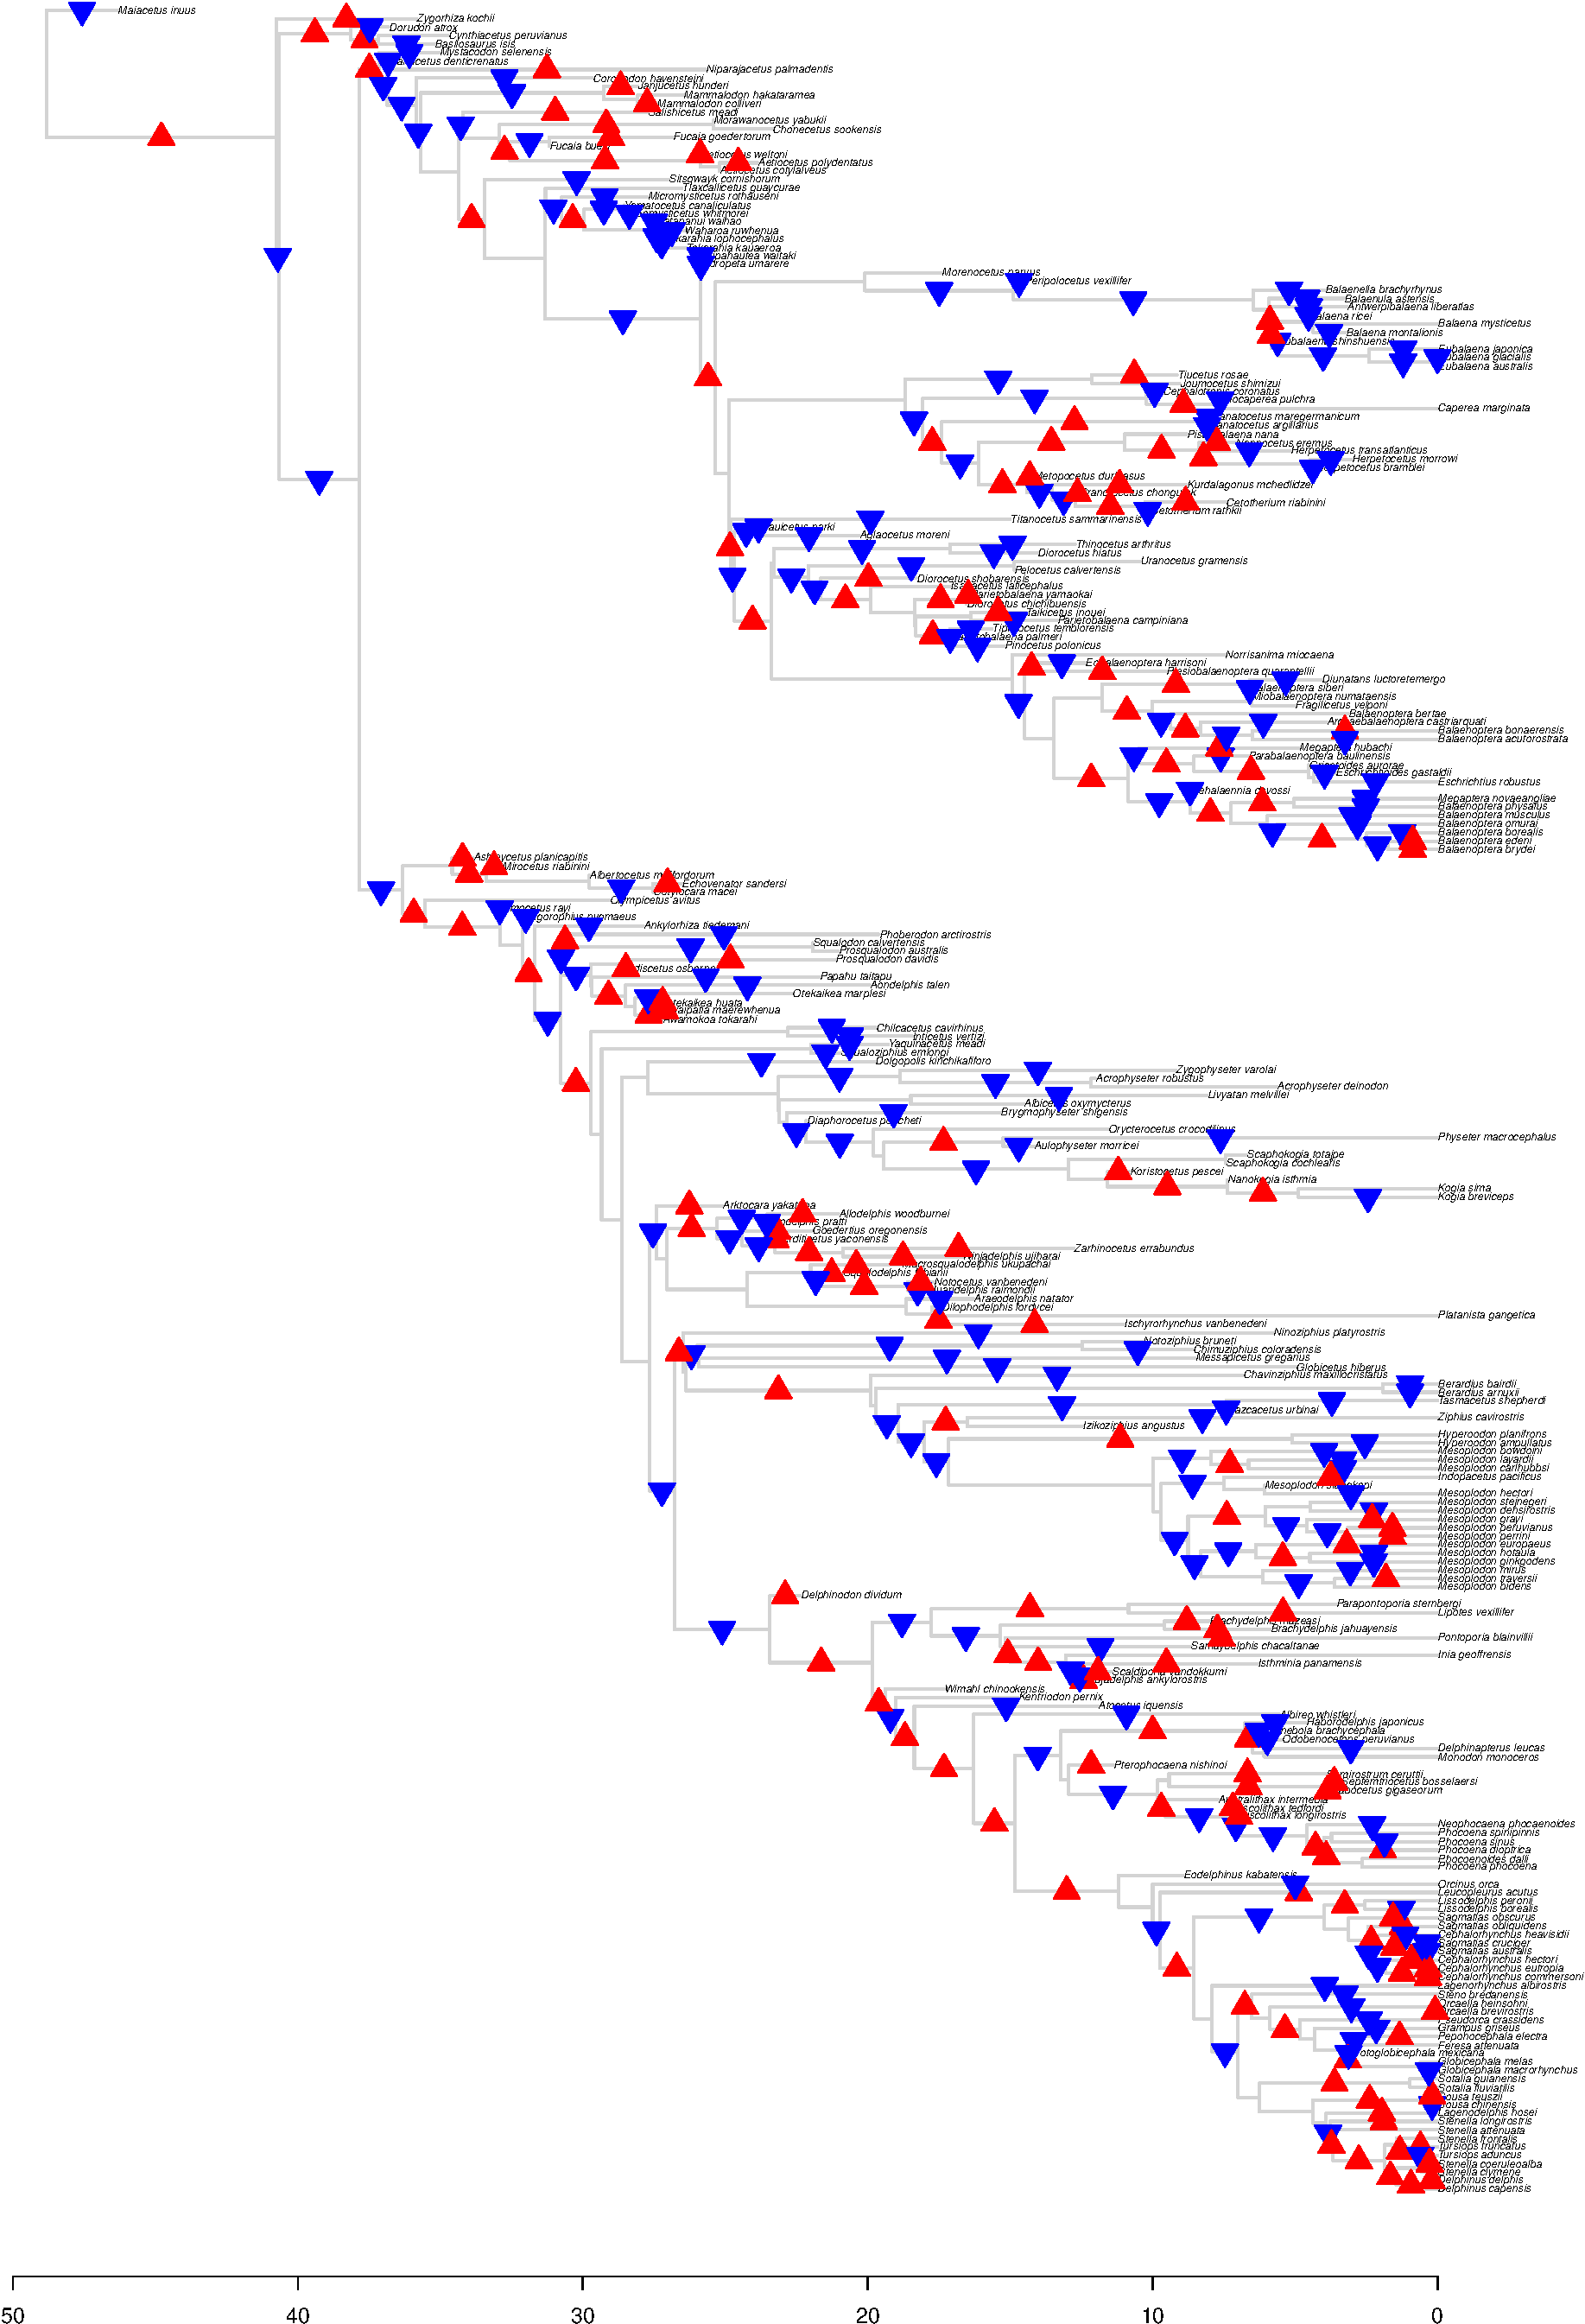
\includegraphics[width=0.9\textwidth]{img/plots-noimput-wZBL-k250-1.pdf}
\caption{Results for \textit{bayou} fit for the \textit{No Imput} tree setting the average number of shifts in the prior distribution ($\lambda$) to 250. The triangles represent the position and direction of the shifts with posterior probability higher than 0.1, with upward triangles (in red) indicating increases in $\theta$, and downward triangles (in blue) indicating decreases in $\theta$.}
\label{fig:noimput-k250}
\end{figure}

\newpage

\begin{figure}[H]
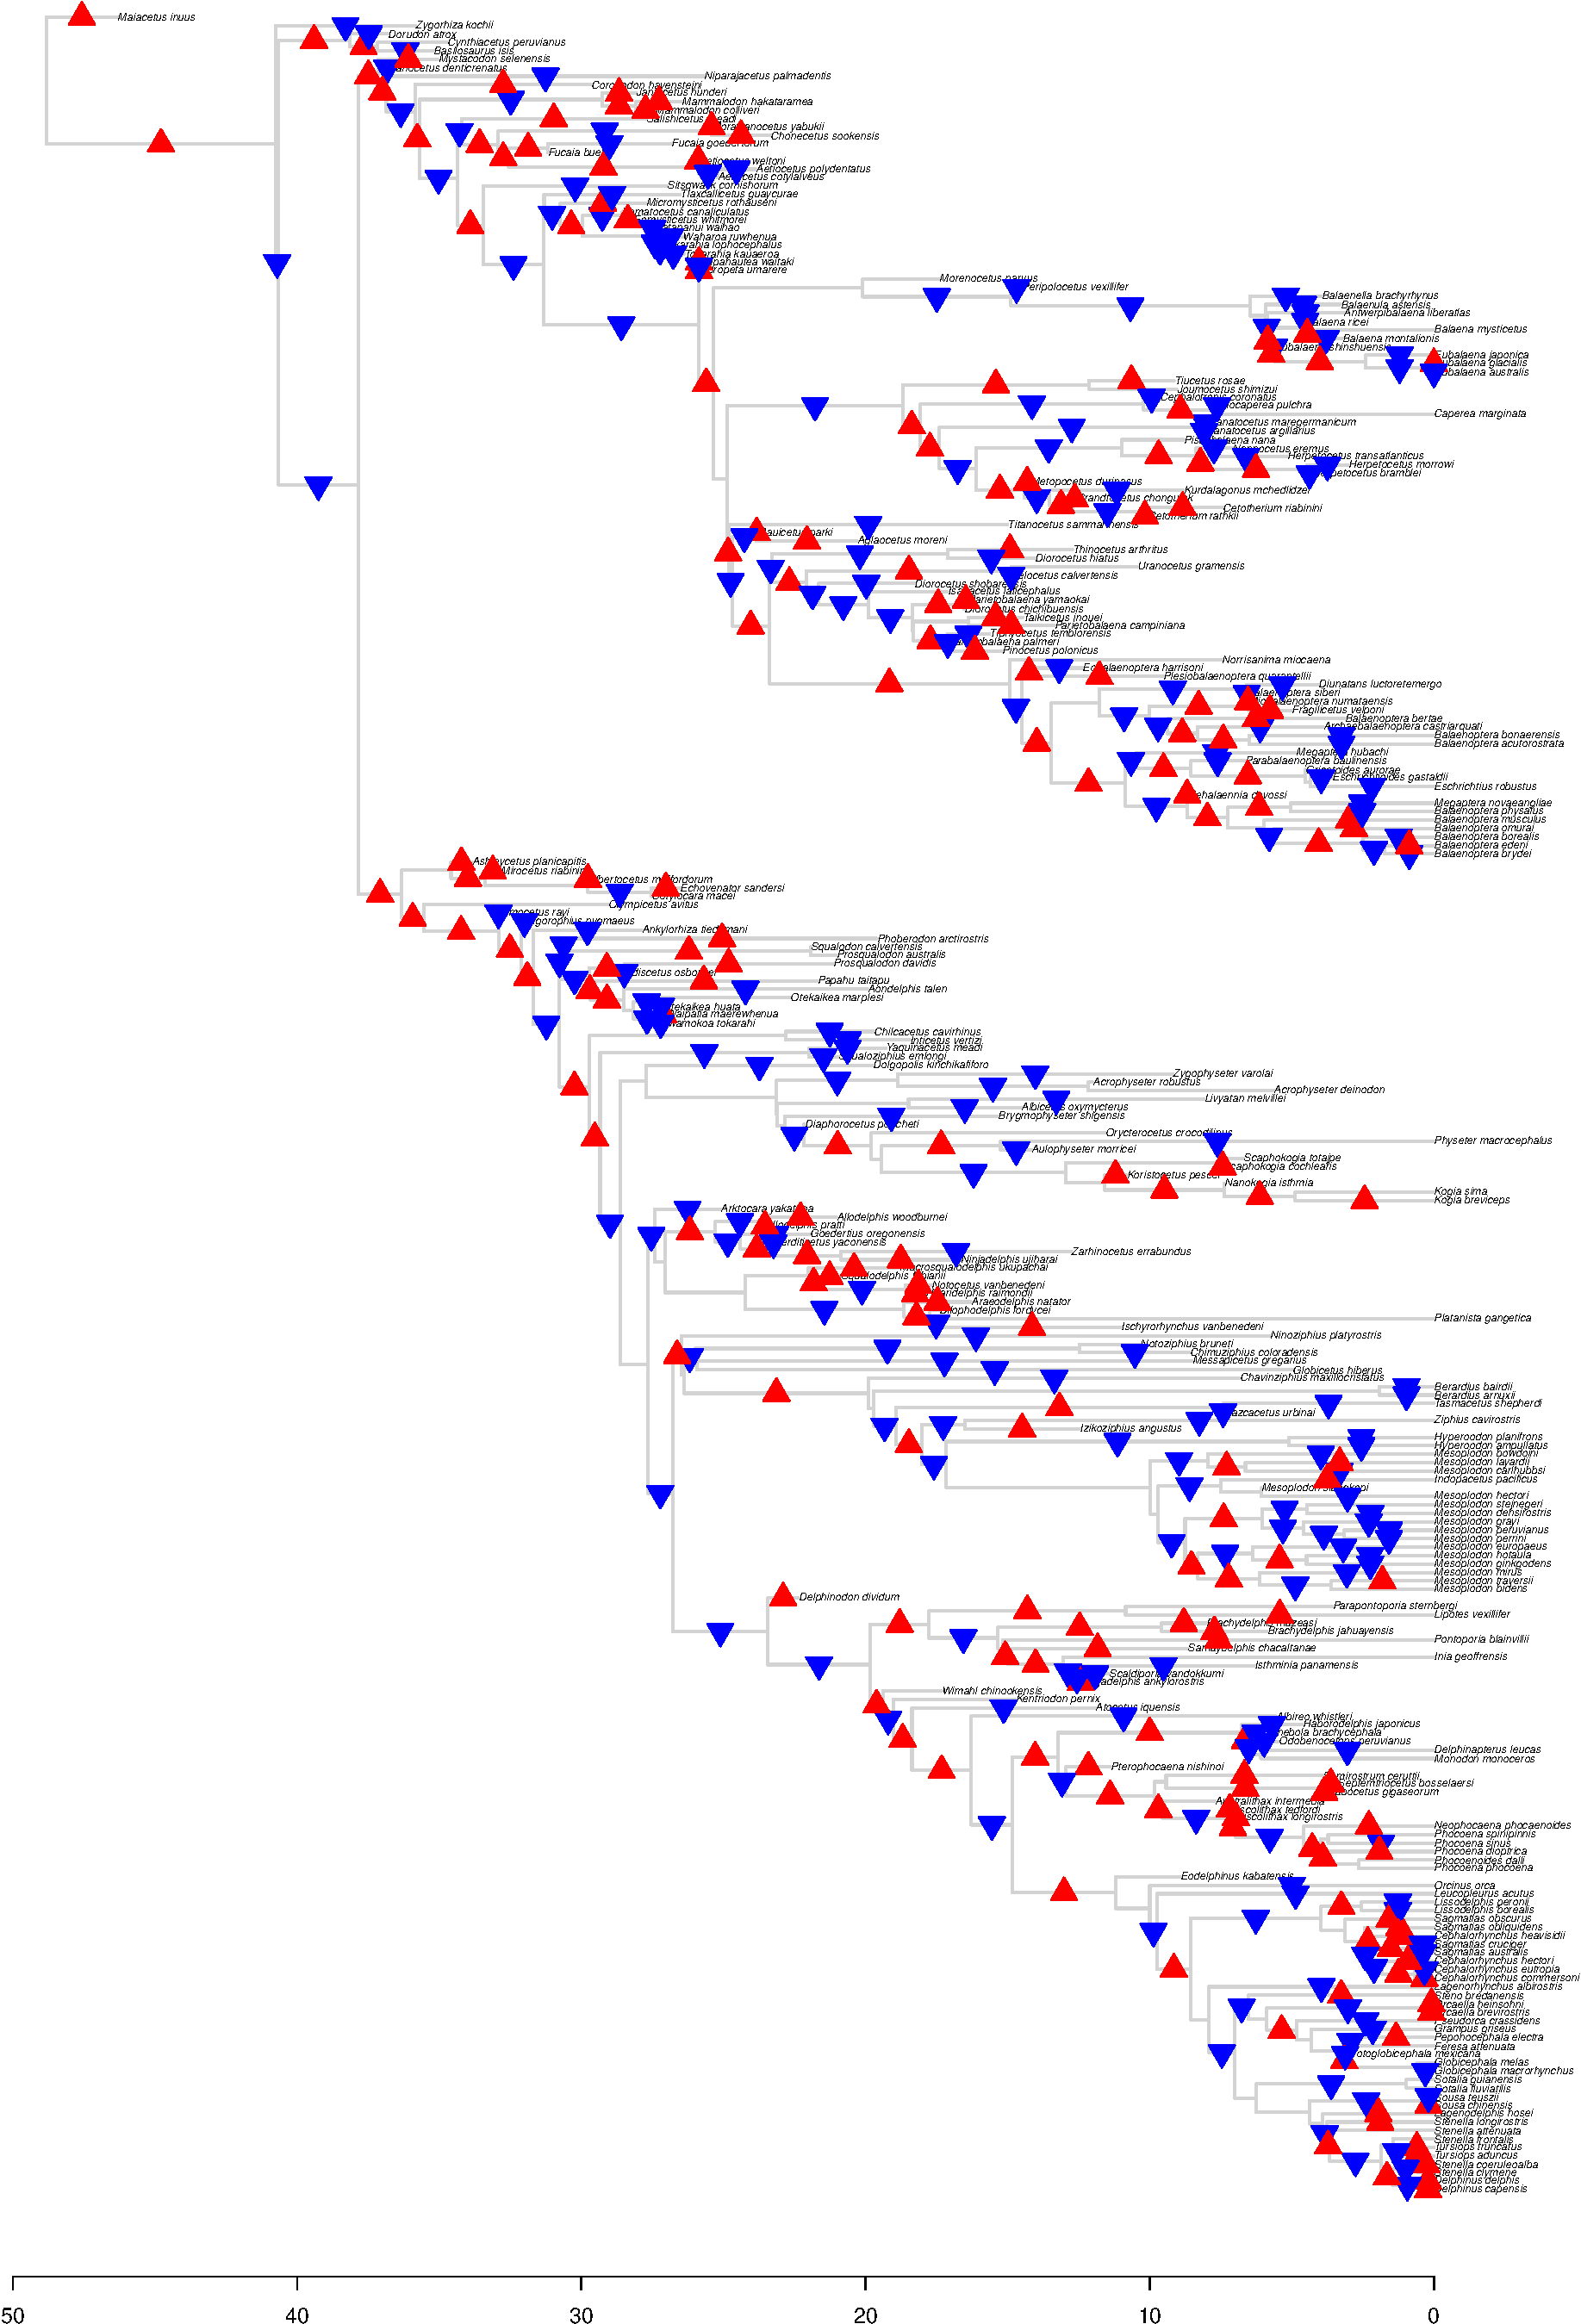
\includegraphics[width=0.9\textwidth]{img/plots-noimput-wZBL-k500-1.pdf}
\caption{Results for \textit{bayou} fit for the \textit{No Imput} tree setting the average number of shifts in the prior distribution ($\lambda$) to 500. The triangles represent the position and direction of the shifts with posterior probability higher than 0.1, with upward triangles (in red) indicating increases in $\theta$, and downward triangles (in blue) indicating decreases in $\theta$.}
\label{fig:noimput-k500}
\end{figure}

%---------------------------------------------------------------------
\subsubsection{\textit{Extant} tree}
%---------------------------------------------------------------------
\begin{figure}[H]
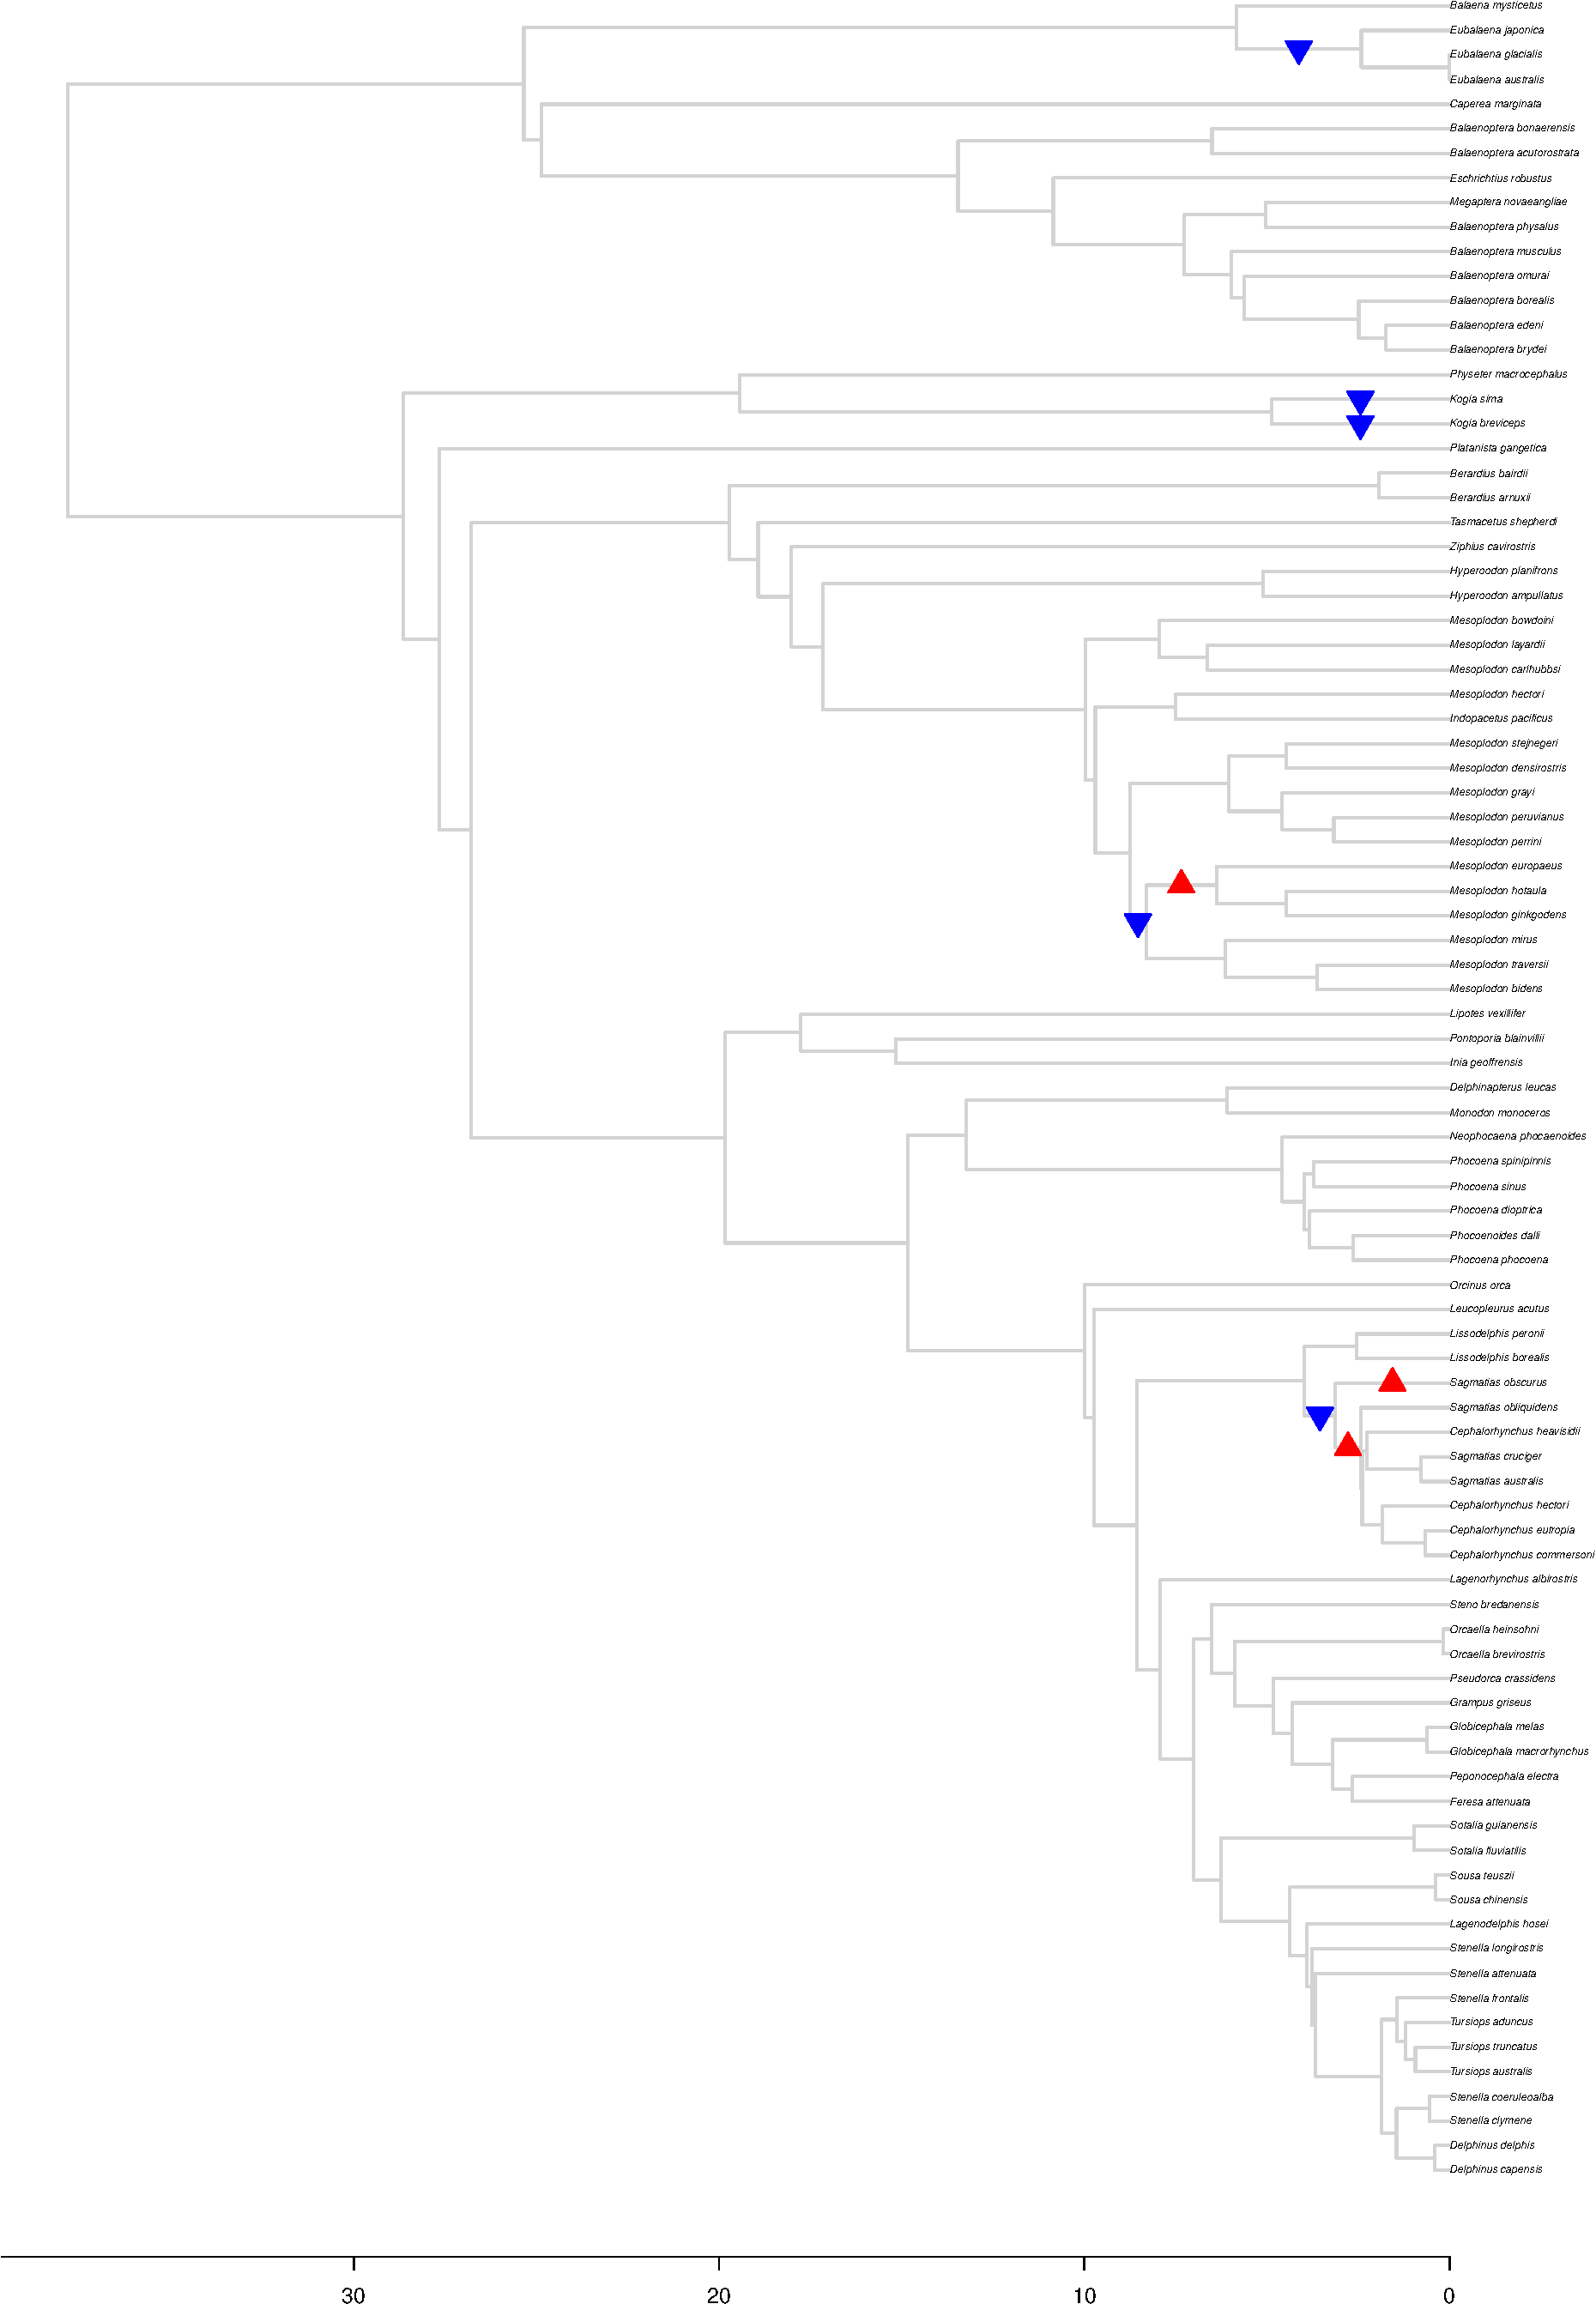
\includegraphics[width=0.9\textwidth]{img/plots-extant-k5-1.pdf}
\caption{Results for \textit{bayou} fit for the \textit{Extant} tree setting the average number of shifts in the prior distribution ($\lambda$) to 5. The triangles represent the position and direction of the shifts with posterior probability higher than 0.1, with upward triangles (in red) indicating increases in $\theta$, and downward triangles (in blue) indicating decreases in $\theta$..}
\label{fig:extant-k5}
\end{figure}

\newpage

\begin{figure}[H]
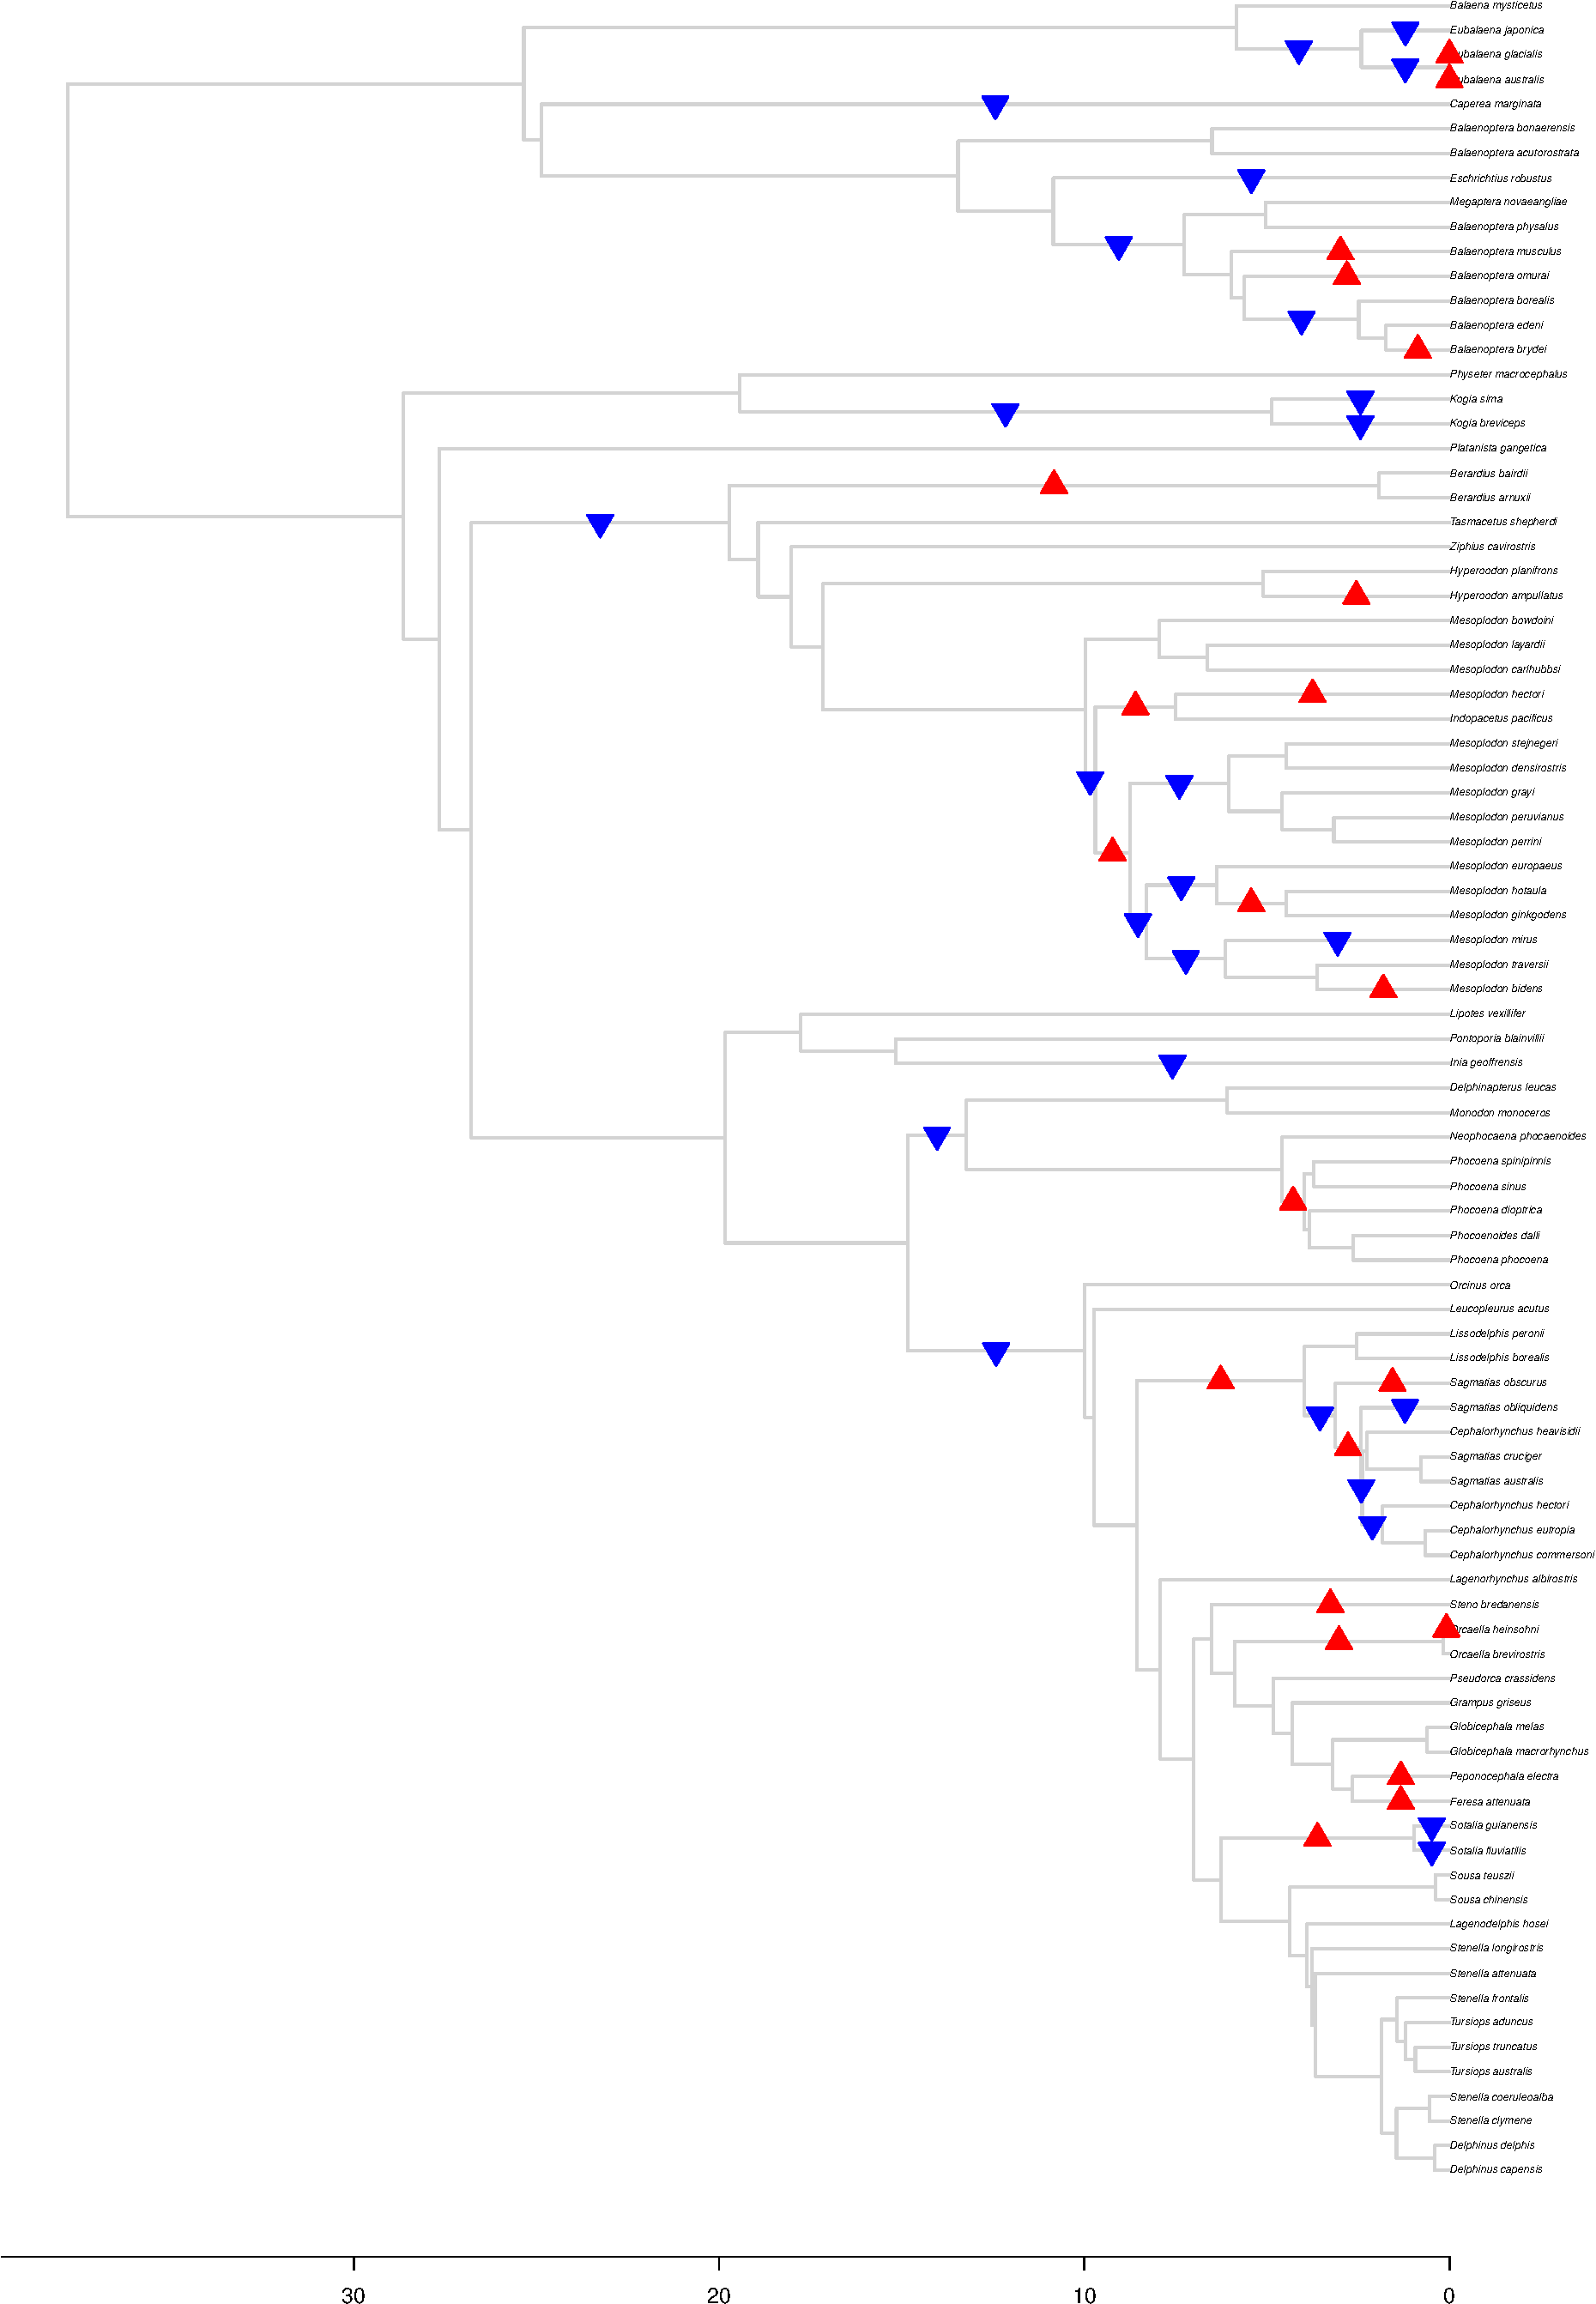
\includegraphics[width=0.9\textwidth]{img/plots-extant-k15-1.pdf}
\caption{Results for \textit{bayou} fit for the \textit{Extant} tree setting the average number of shifts in the prior distribution ($\lambda$) to 15. The triangles represent the position and direction of the shifts with posterior probability higher than 0.1, with upward triangles (in red) indicating increases in $\theta$, and downward triangles (in blue) indicating decreases in $\theta$.}
\label{fig:extant-k15}
\end{figure}

\newpage

\begin{figure}[H]
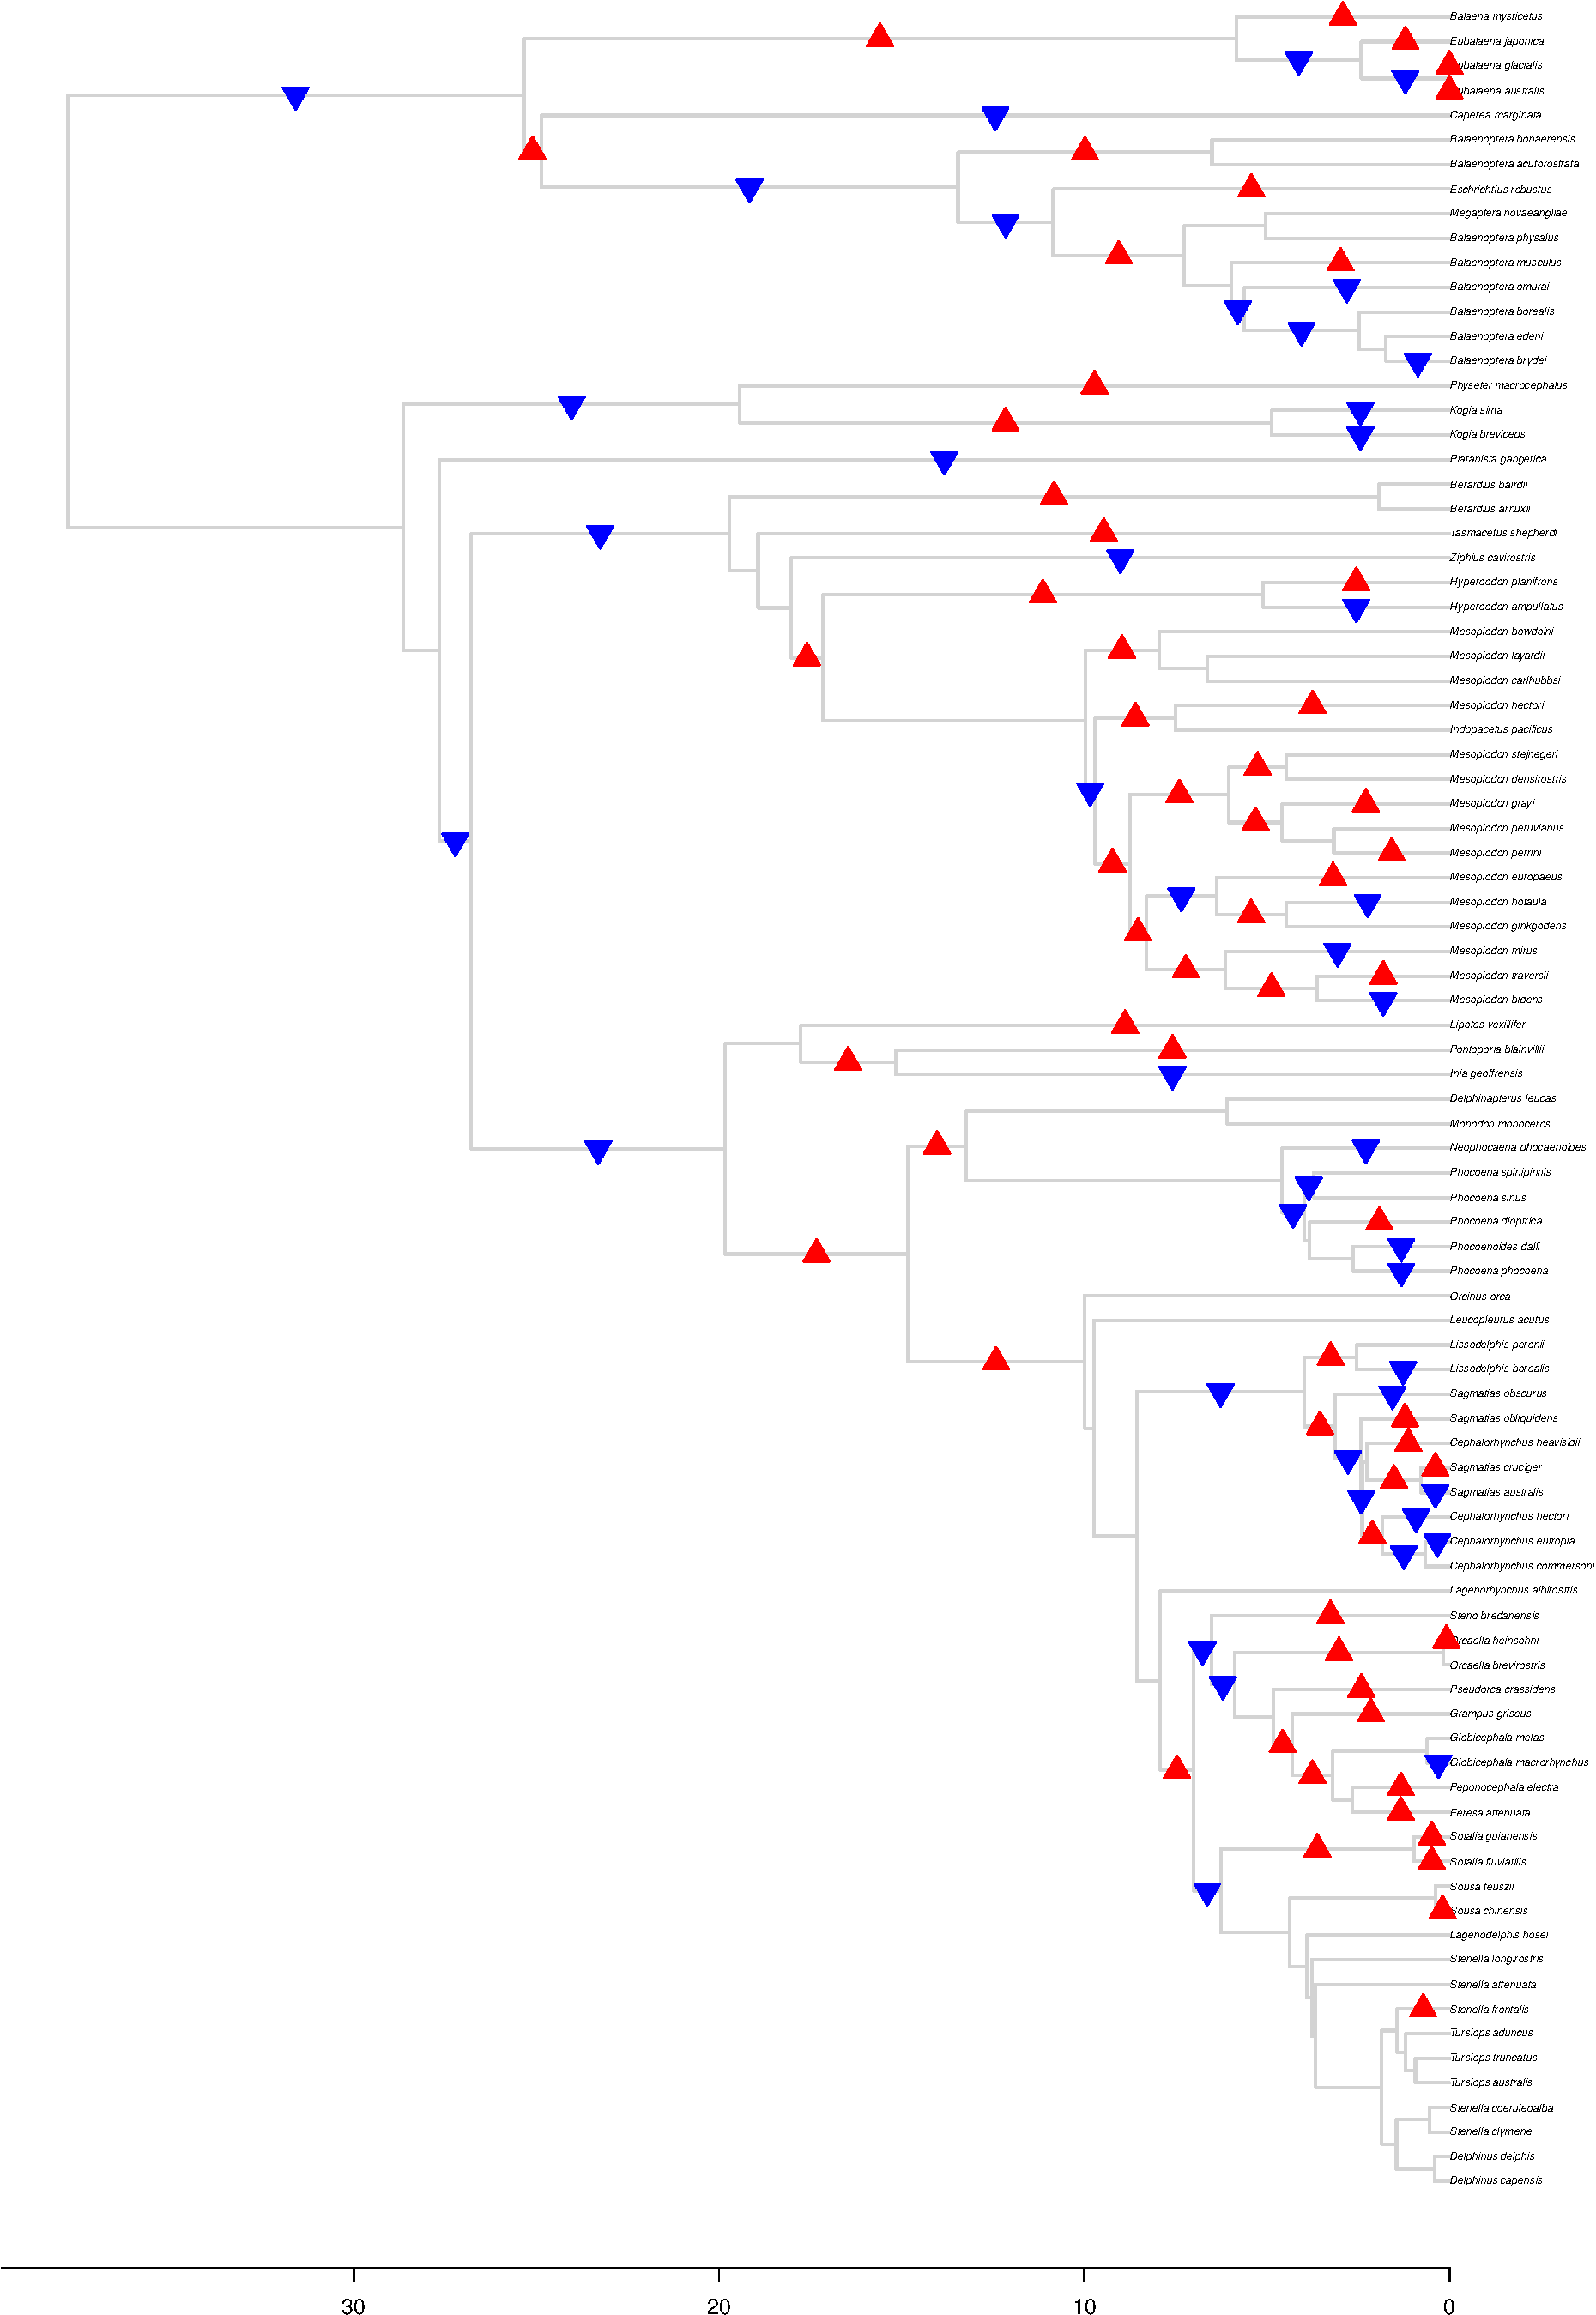
\includegraphics[width=0.9\textwidth]{img/plots-extant-k50-1.pdf}
\caption{Results for \textit{bayou} fit for the \textit{Extant} tree setting the average number of shifts in the prior distribution ($\lambda$) to 50. The triangles represent the position and direction of the shifts with posterior probability higher than 0.1, with upward triangles (in red) indicating increases in $\theta$, and downward triangles (in blue) indicating decreases in $\theta$.}
\label{fig:extant-k50}
\end{figure}

%---------------------------------------------------------------------
\subsubsection{\textit{Baleen} tree}
%---------------------------------------------------------------------
\begin{figure}[H]
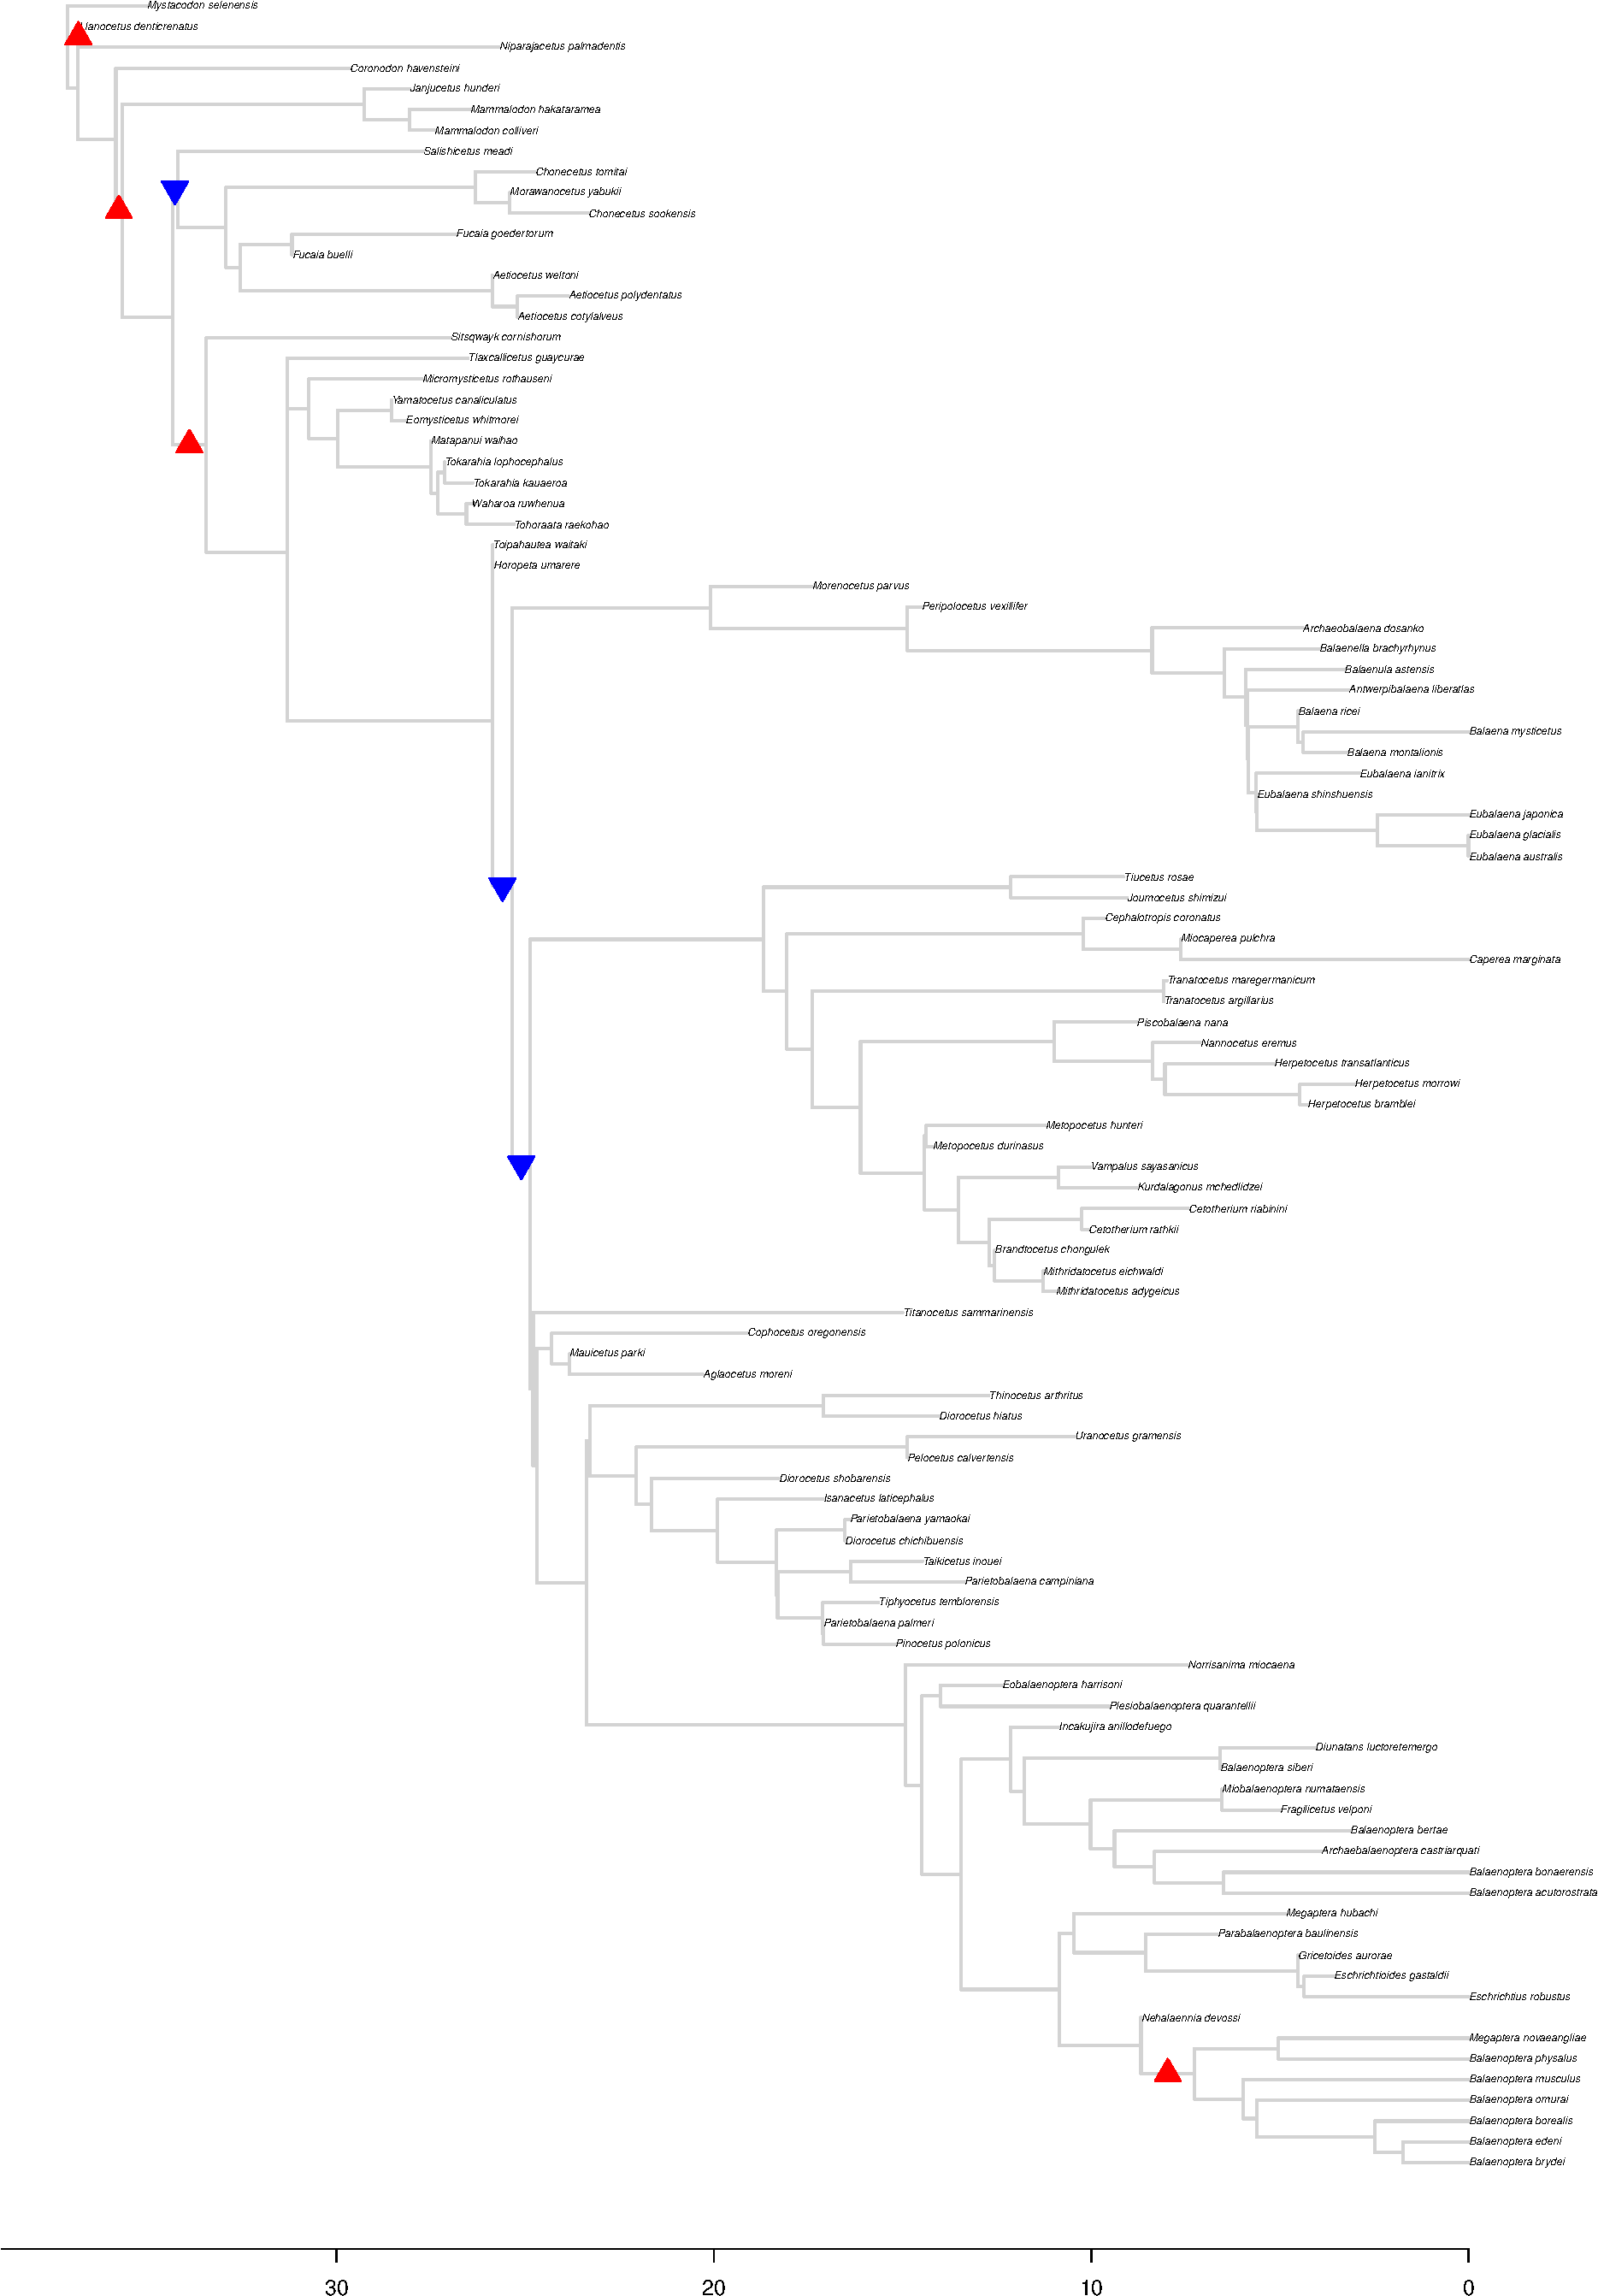
\includegraphics[width=0.9\textwidth]{img/plots-baleen-wZBL-k5-1.pdf}
\caption{Results for \textit{bayou} fit for the \textit{Baleen} tree setting the average number of shifts in the prior distribution ($\lambda$) to 5. The triangles represent the position and direction of the shifts with posterior probability higher than 0.1, with upward triangles (in red) indicating increases in $\theta$, and downward triangles (in blue) indicating decreases in $\theta$.}
\label{fig:baleen-k5}
\end{figure}

\newpage

\begin{figure}[H]
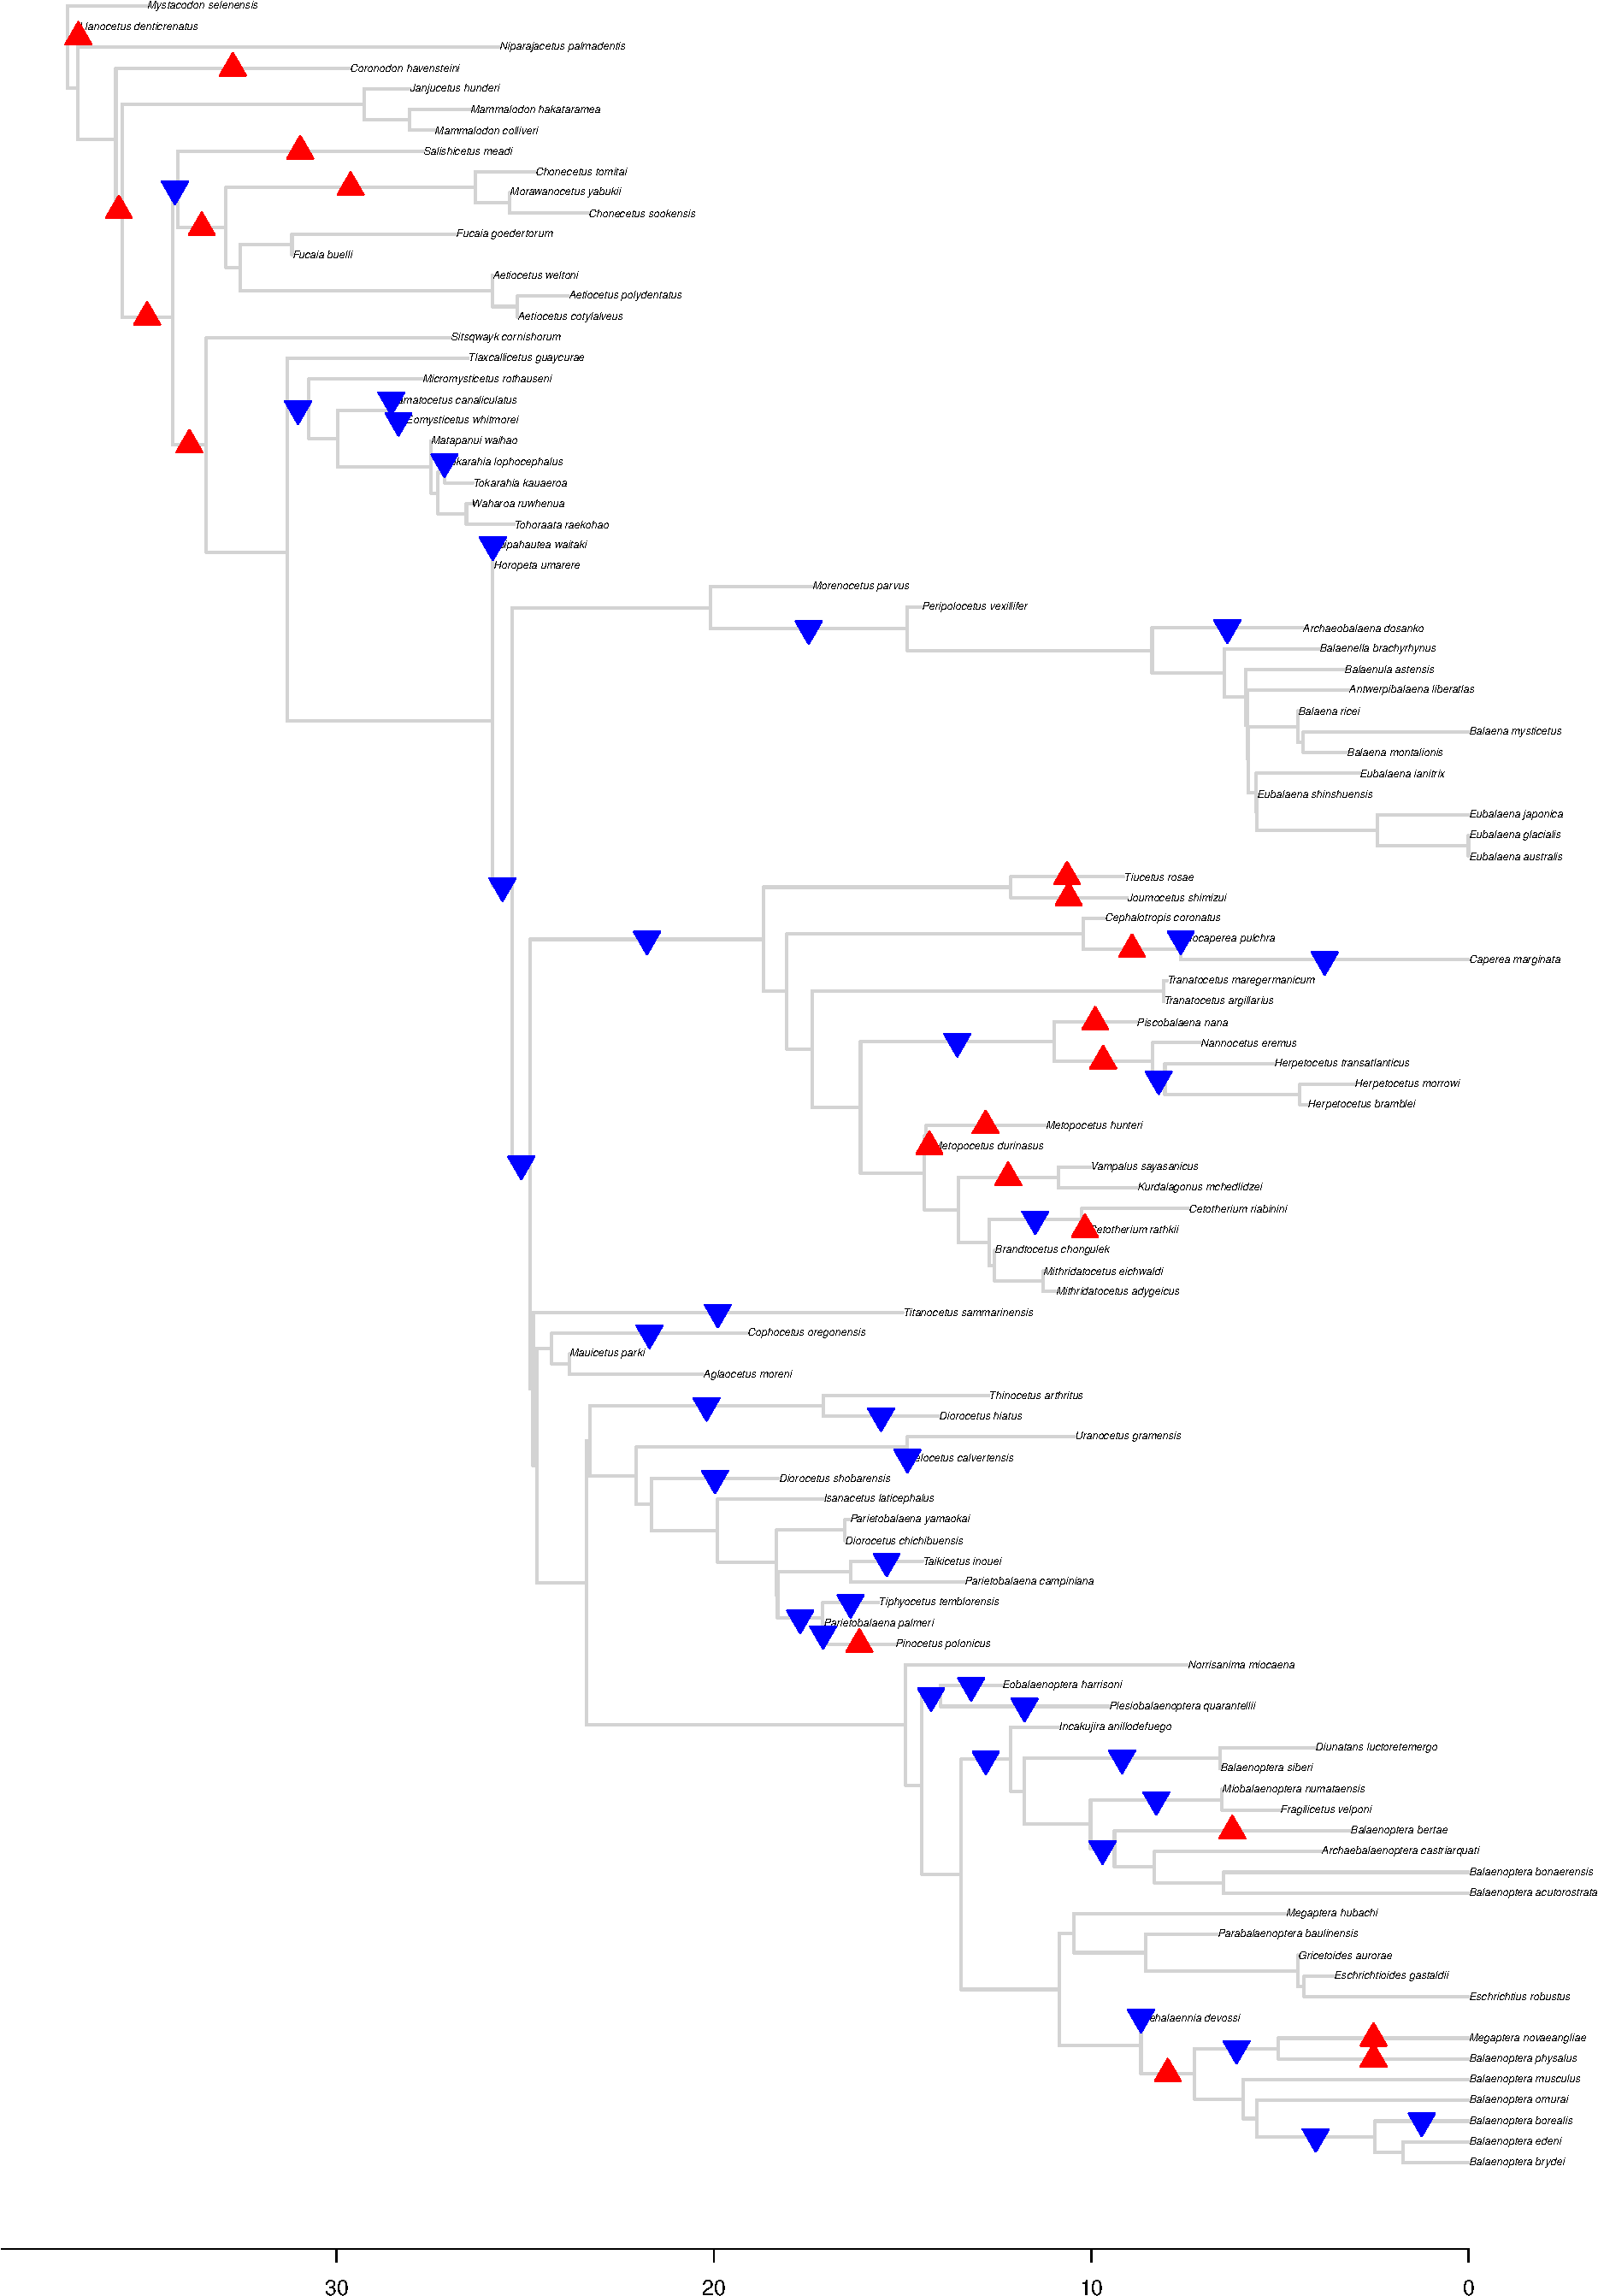
\includegraphics[width=0.9\textwidth]{img/plots-baleen-wZBL-k15-1.pdf}
\caption{Results for \textit{bayou} fit for the \textit{Baleen} tree setting the average number of shifts in the prior distribution ($\lambda$) to 15. The triangles represent the position and direction of the shifts with posterior probability higher than 0.1, with upward triangles (in red) indicating increases in $\theta$, and downward triangles (in blue) indicating decreases in $\theta$.}
\label{fig:baleen-k15}
\end{figure}

\newpage

\begin{figure}[H]
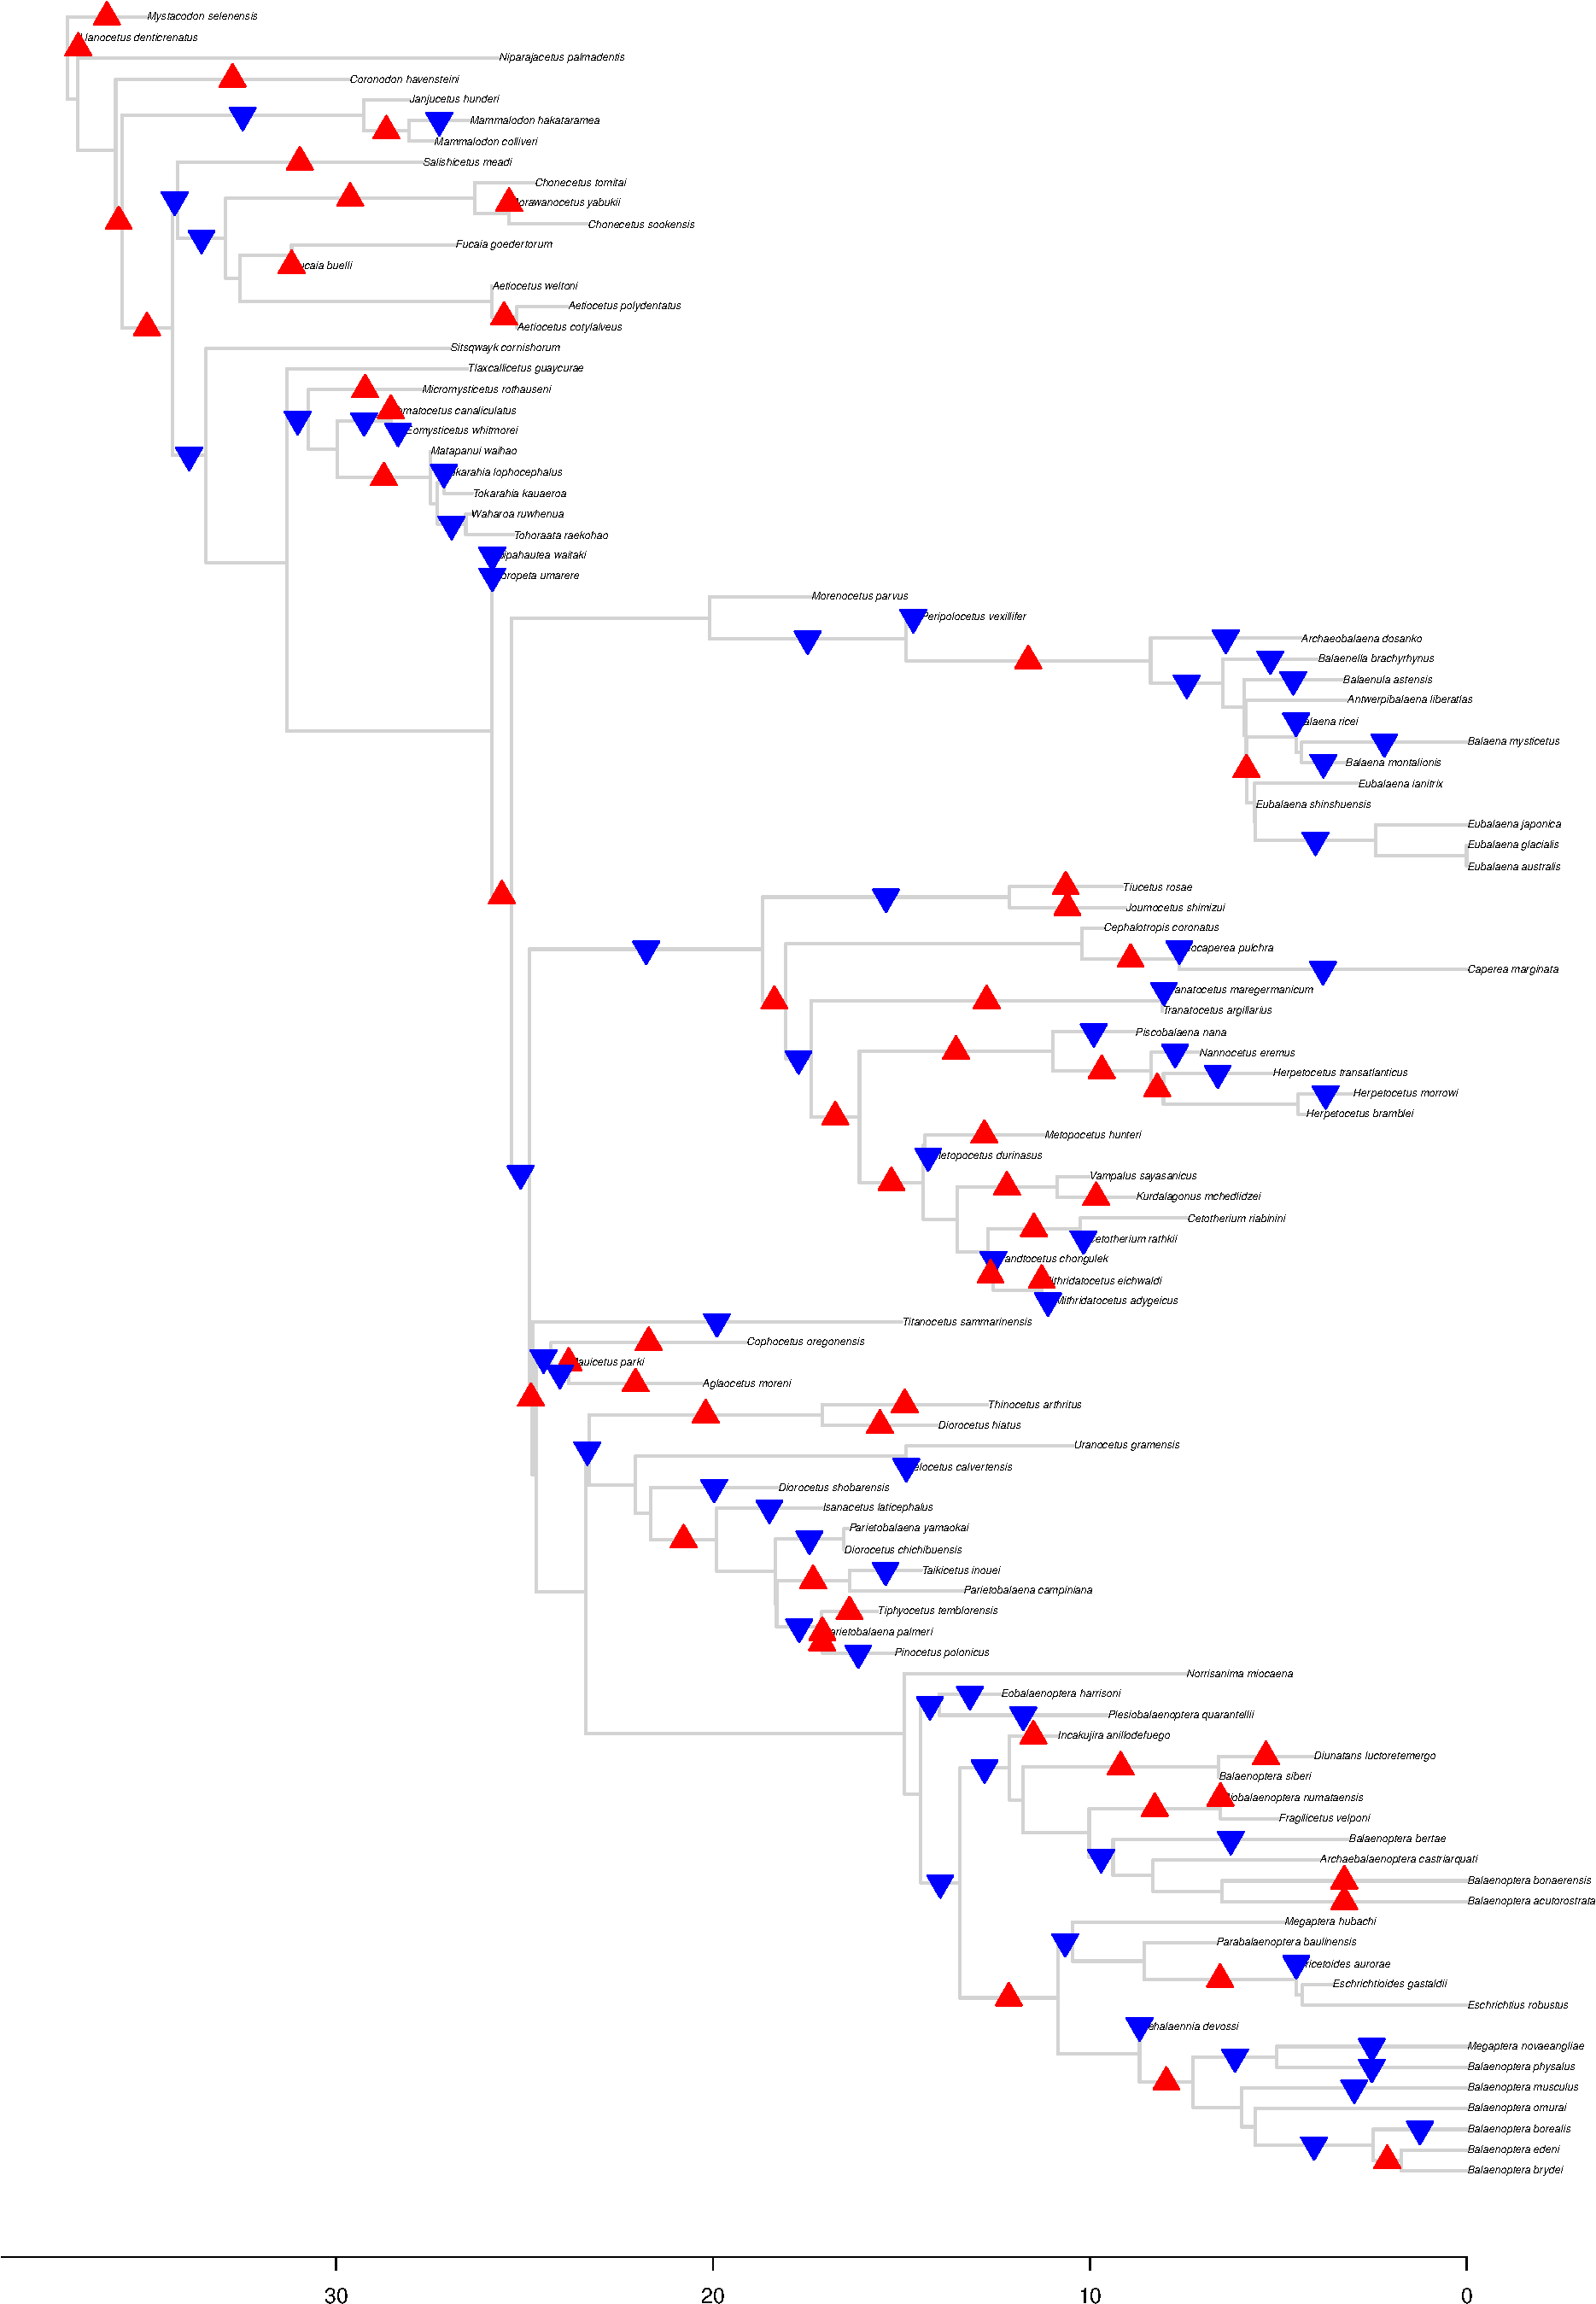
\includegraphics[width=0.9\textwidth]{img/plots-baleen-wZBL-k50-1.pdf}
\caption{Results for \textit{bayou} fit for the \textit{Baleen} tree setting the average number of shifts in the prior distribution ($\lambda$) to 50. The triangles represent the position and direction of the shifts with posterior probability higher than 0.1, with upward triangles (in red) indicating increases in $\theta$, and downward triangles (in blue) indicating decreases in $\theta$.}
\label{fig:baleen-k50}
\end{figure}

%---------------------------------------------------------------------
\subsubsection{\textit{Toothed} tree}
%---------------------------------------------------------------------

\begin{figure}[H]
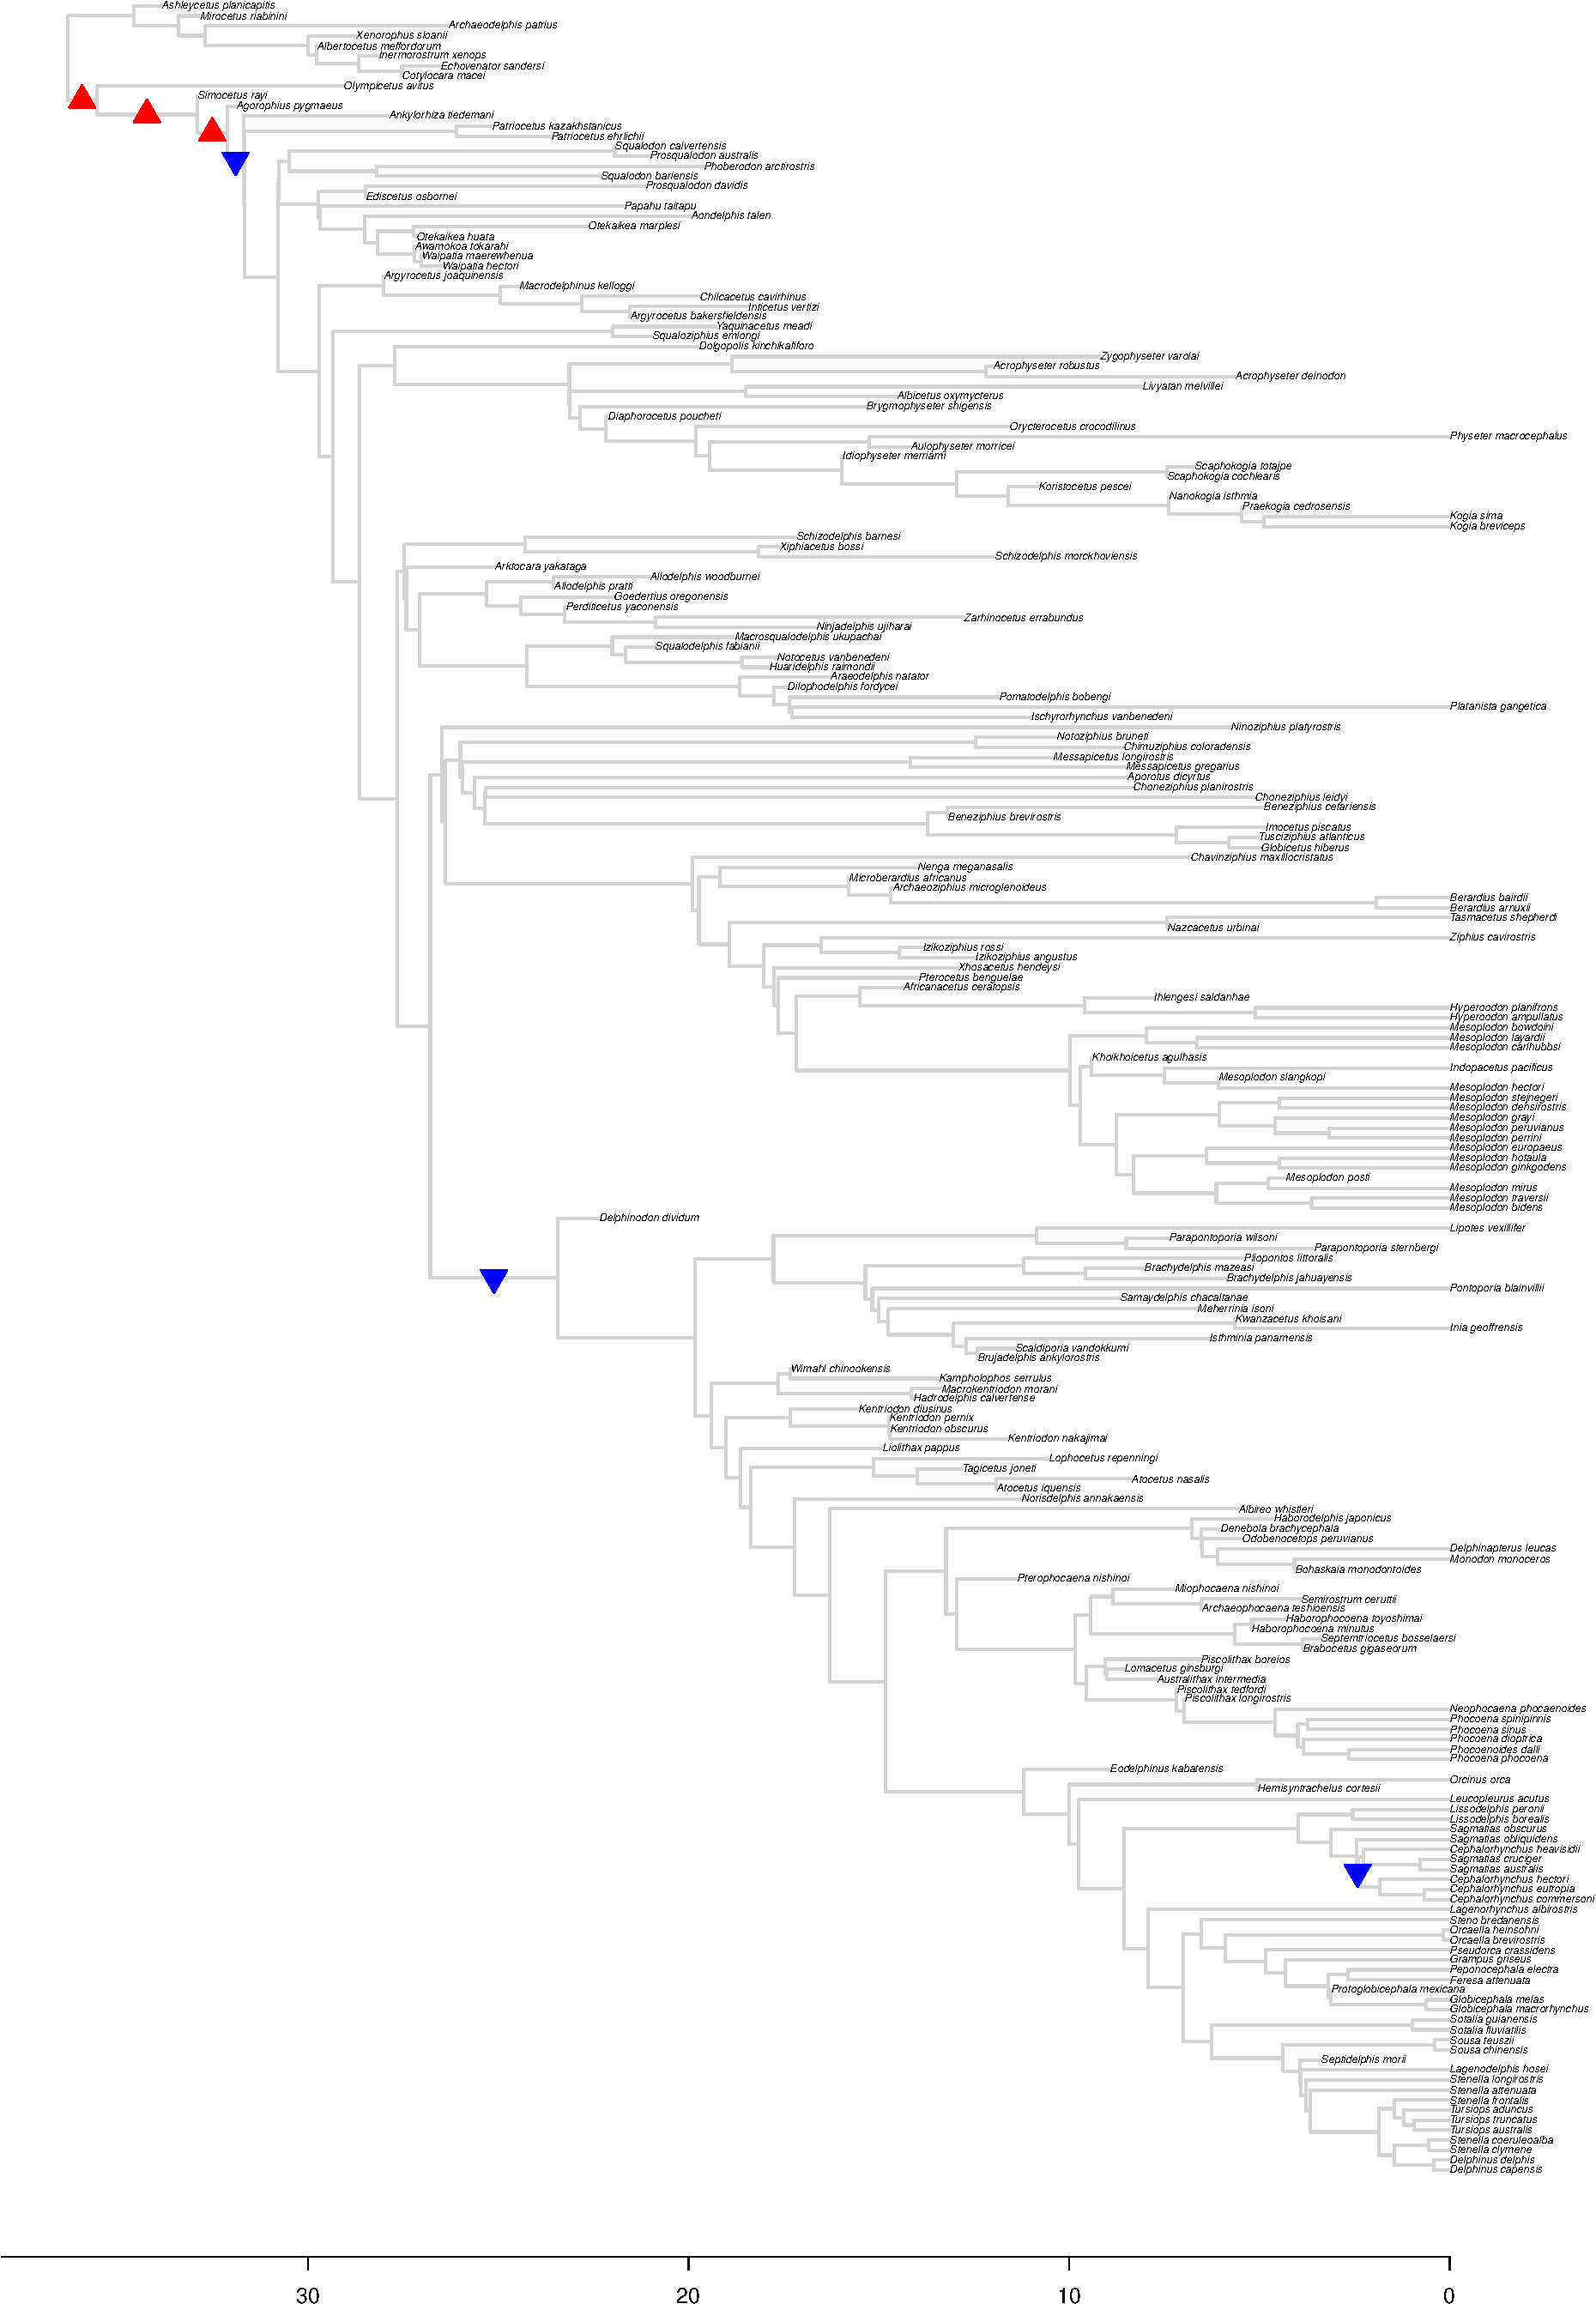
\includegraphics[width=0.9\textwidth]{img/plots-toothed-wZBL-k5-1.pdf}
\caption{Results for \textit{bayou} fit for the \textit{Toothed} tree setting the average number of shifts in the prior distribution ($\lambda$) to 5. The triangles represent the position and direction of the shifts with posterior probability higher than 0.1, with upward triangles (in red) indicating increases in $\theta$, and downward triangles (in blue) indicating decreases in $\theta$.}
\label{fig:toothed-k5}
\end{figure}

\newpage

\begin{figure}[H]
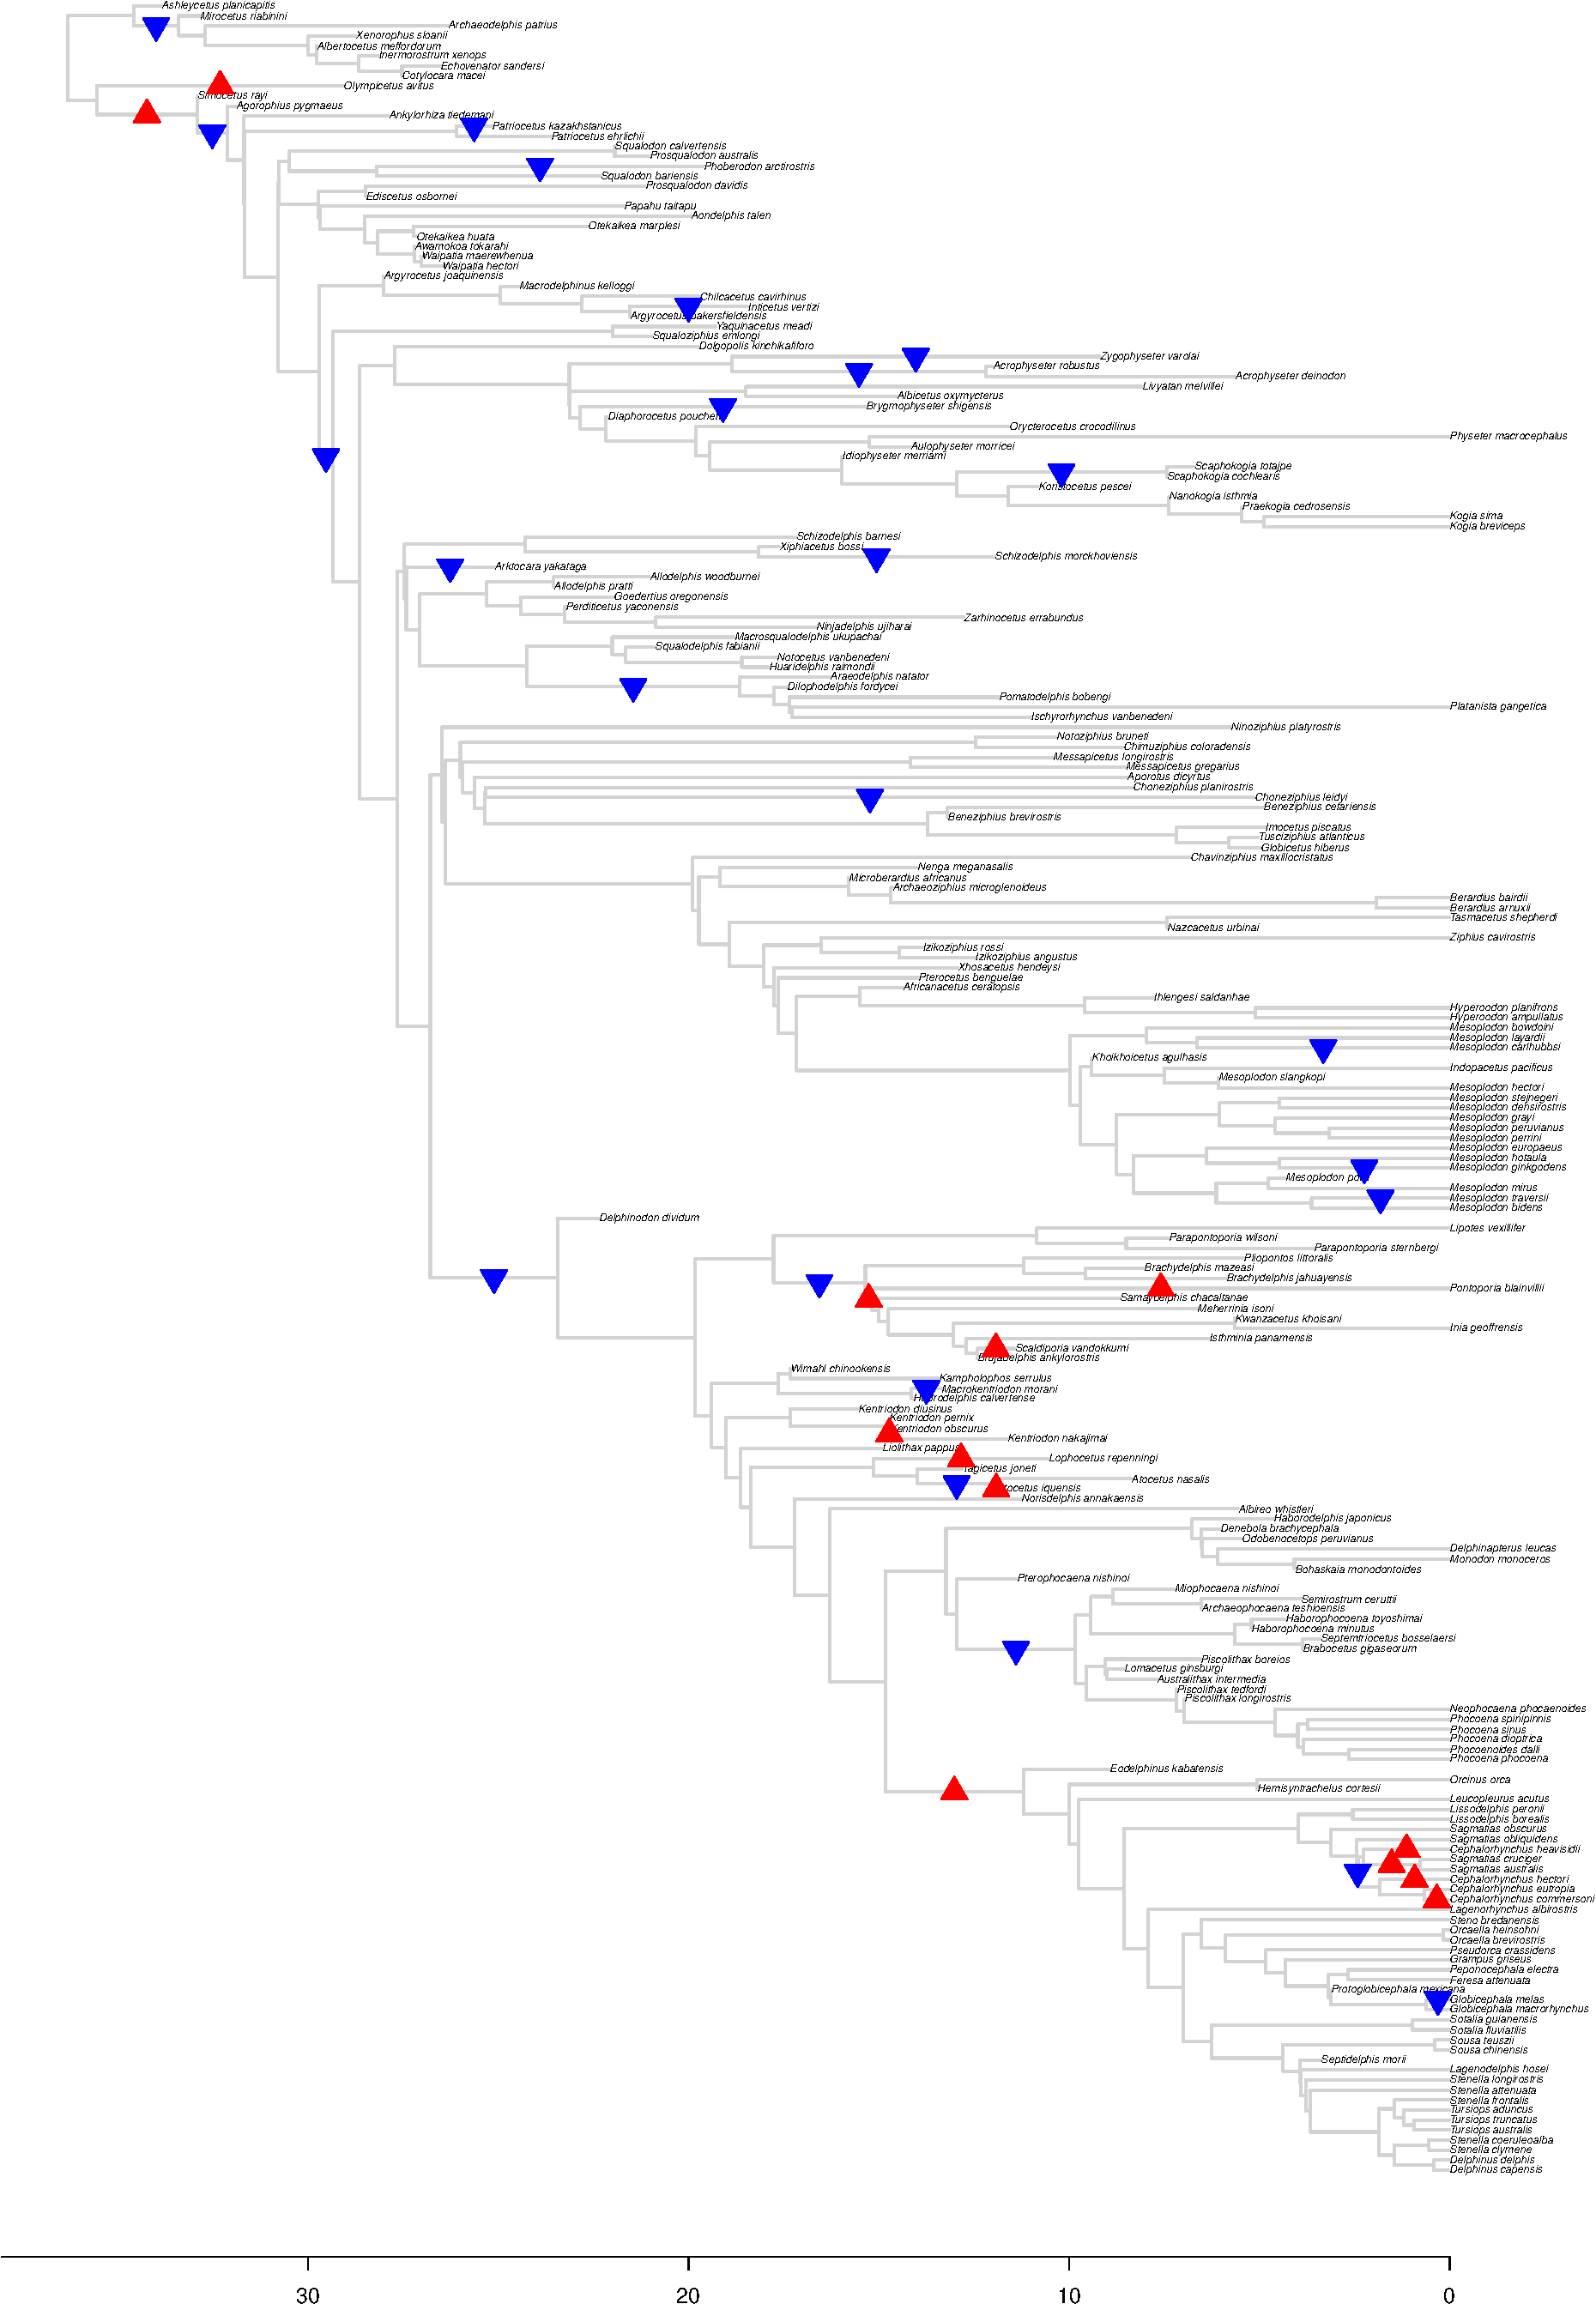
\includegraphics[width=0.9\textwidth]{img/plots-toothed-wZBL-k15-1.pdf}
\caption{Results for \textit{bayou} fit for the \textit{Toothed} tree setting the average number of shifts in the prior distribution ($\lambda$) to 15. The triangles represent the position and direction of the shifts with posterior probability higher than 0.1, with upward triangles (in red) indicating increases in $\theta$, and downward triangles (in blue) indicating decreases in $\theta$.}
\label{fig:toothed-k15}
\end{figure}

\newpage

\begin{figure}[H]
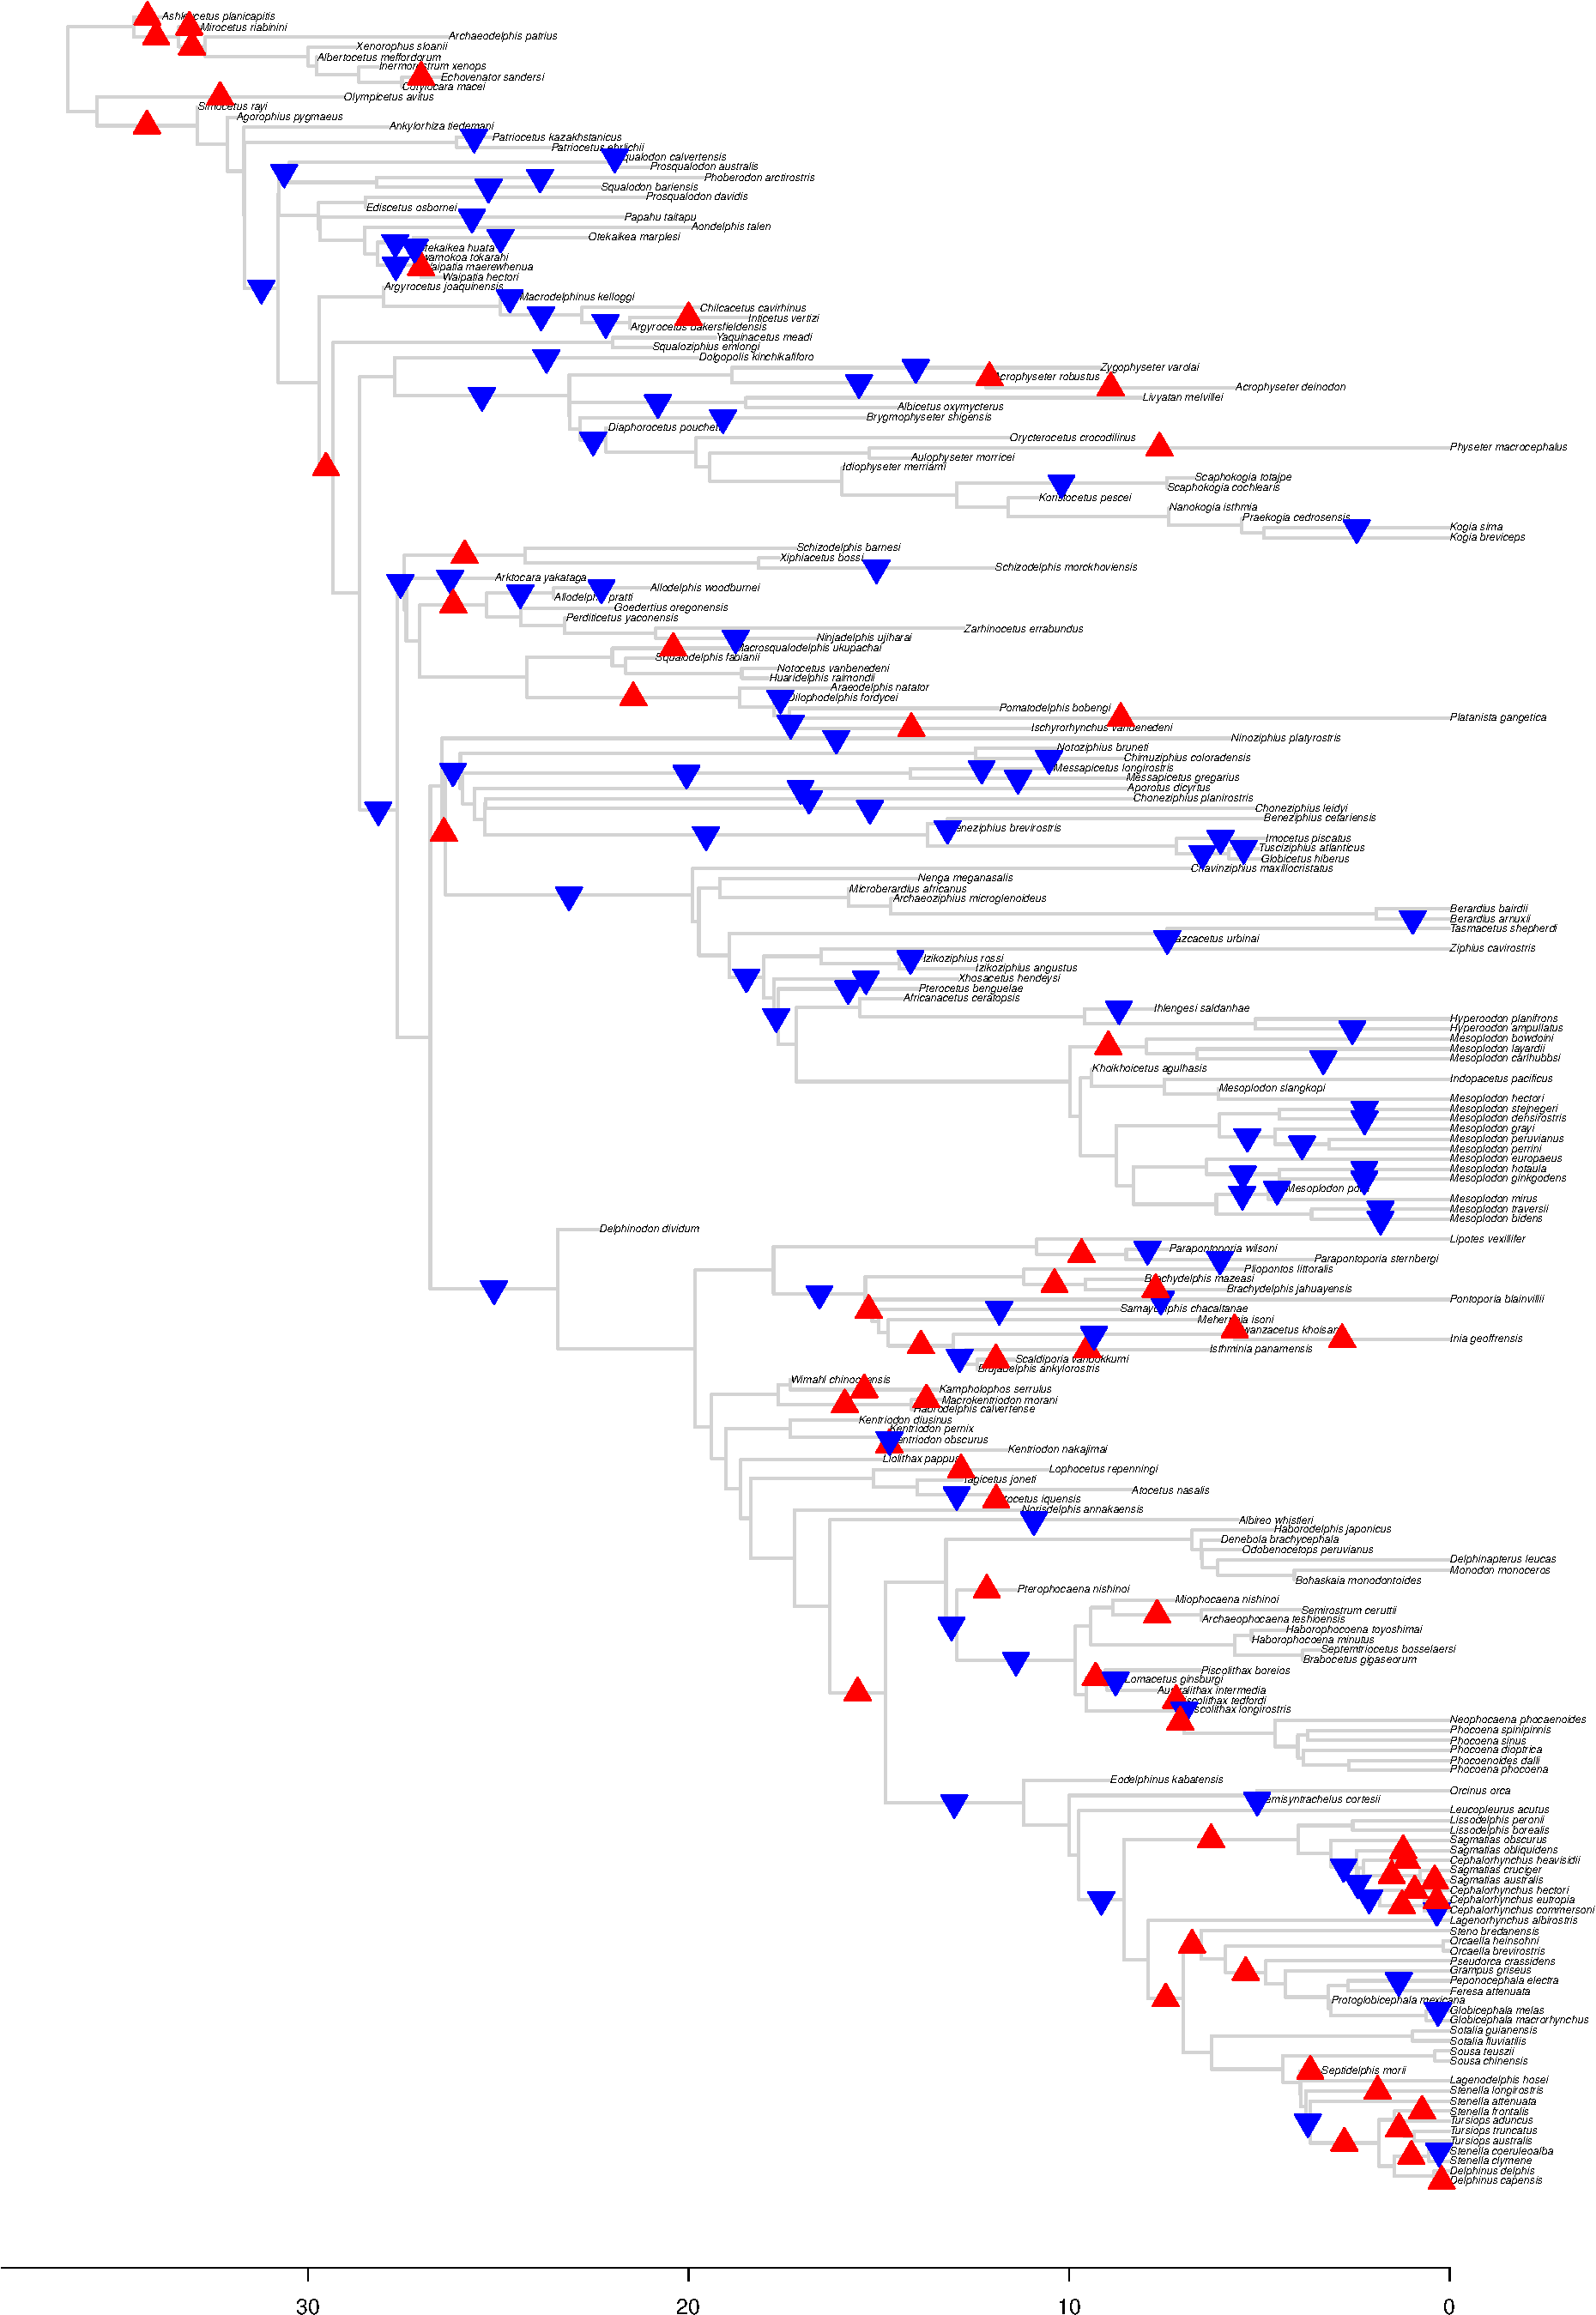
\includegraphics[width=0.9\textwidth]{img/plots-toothed-wZBL-k50-1.pdf}
\caption{Results for \textit{bayou} fit for the \textit{Toothed} tree setting the average number of shifts in the prior distribution ($\lambda$) to 50. The triangles represent the position and direction of the shifts with posterior probability higher than 0.1, with upward triangles (in red) indicating increases in $\theta$, and downward triangles (in blue) indicating decreases in $\theta$.}
\label{fig:toothed-k50}
\end{figure}

%---------------------------------------------------------------------
\subsection{Supplementary Results: Removing taxa with zero-length branches}
%---------------------------------------------------------------------
\subsubsection{\textit{Full} tree}
%---------------------------------------------------------------------

\begin{figure}[H]
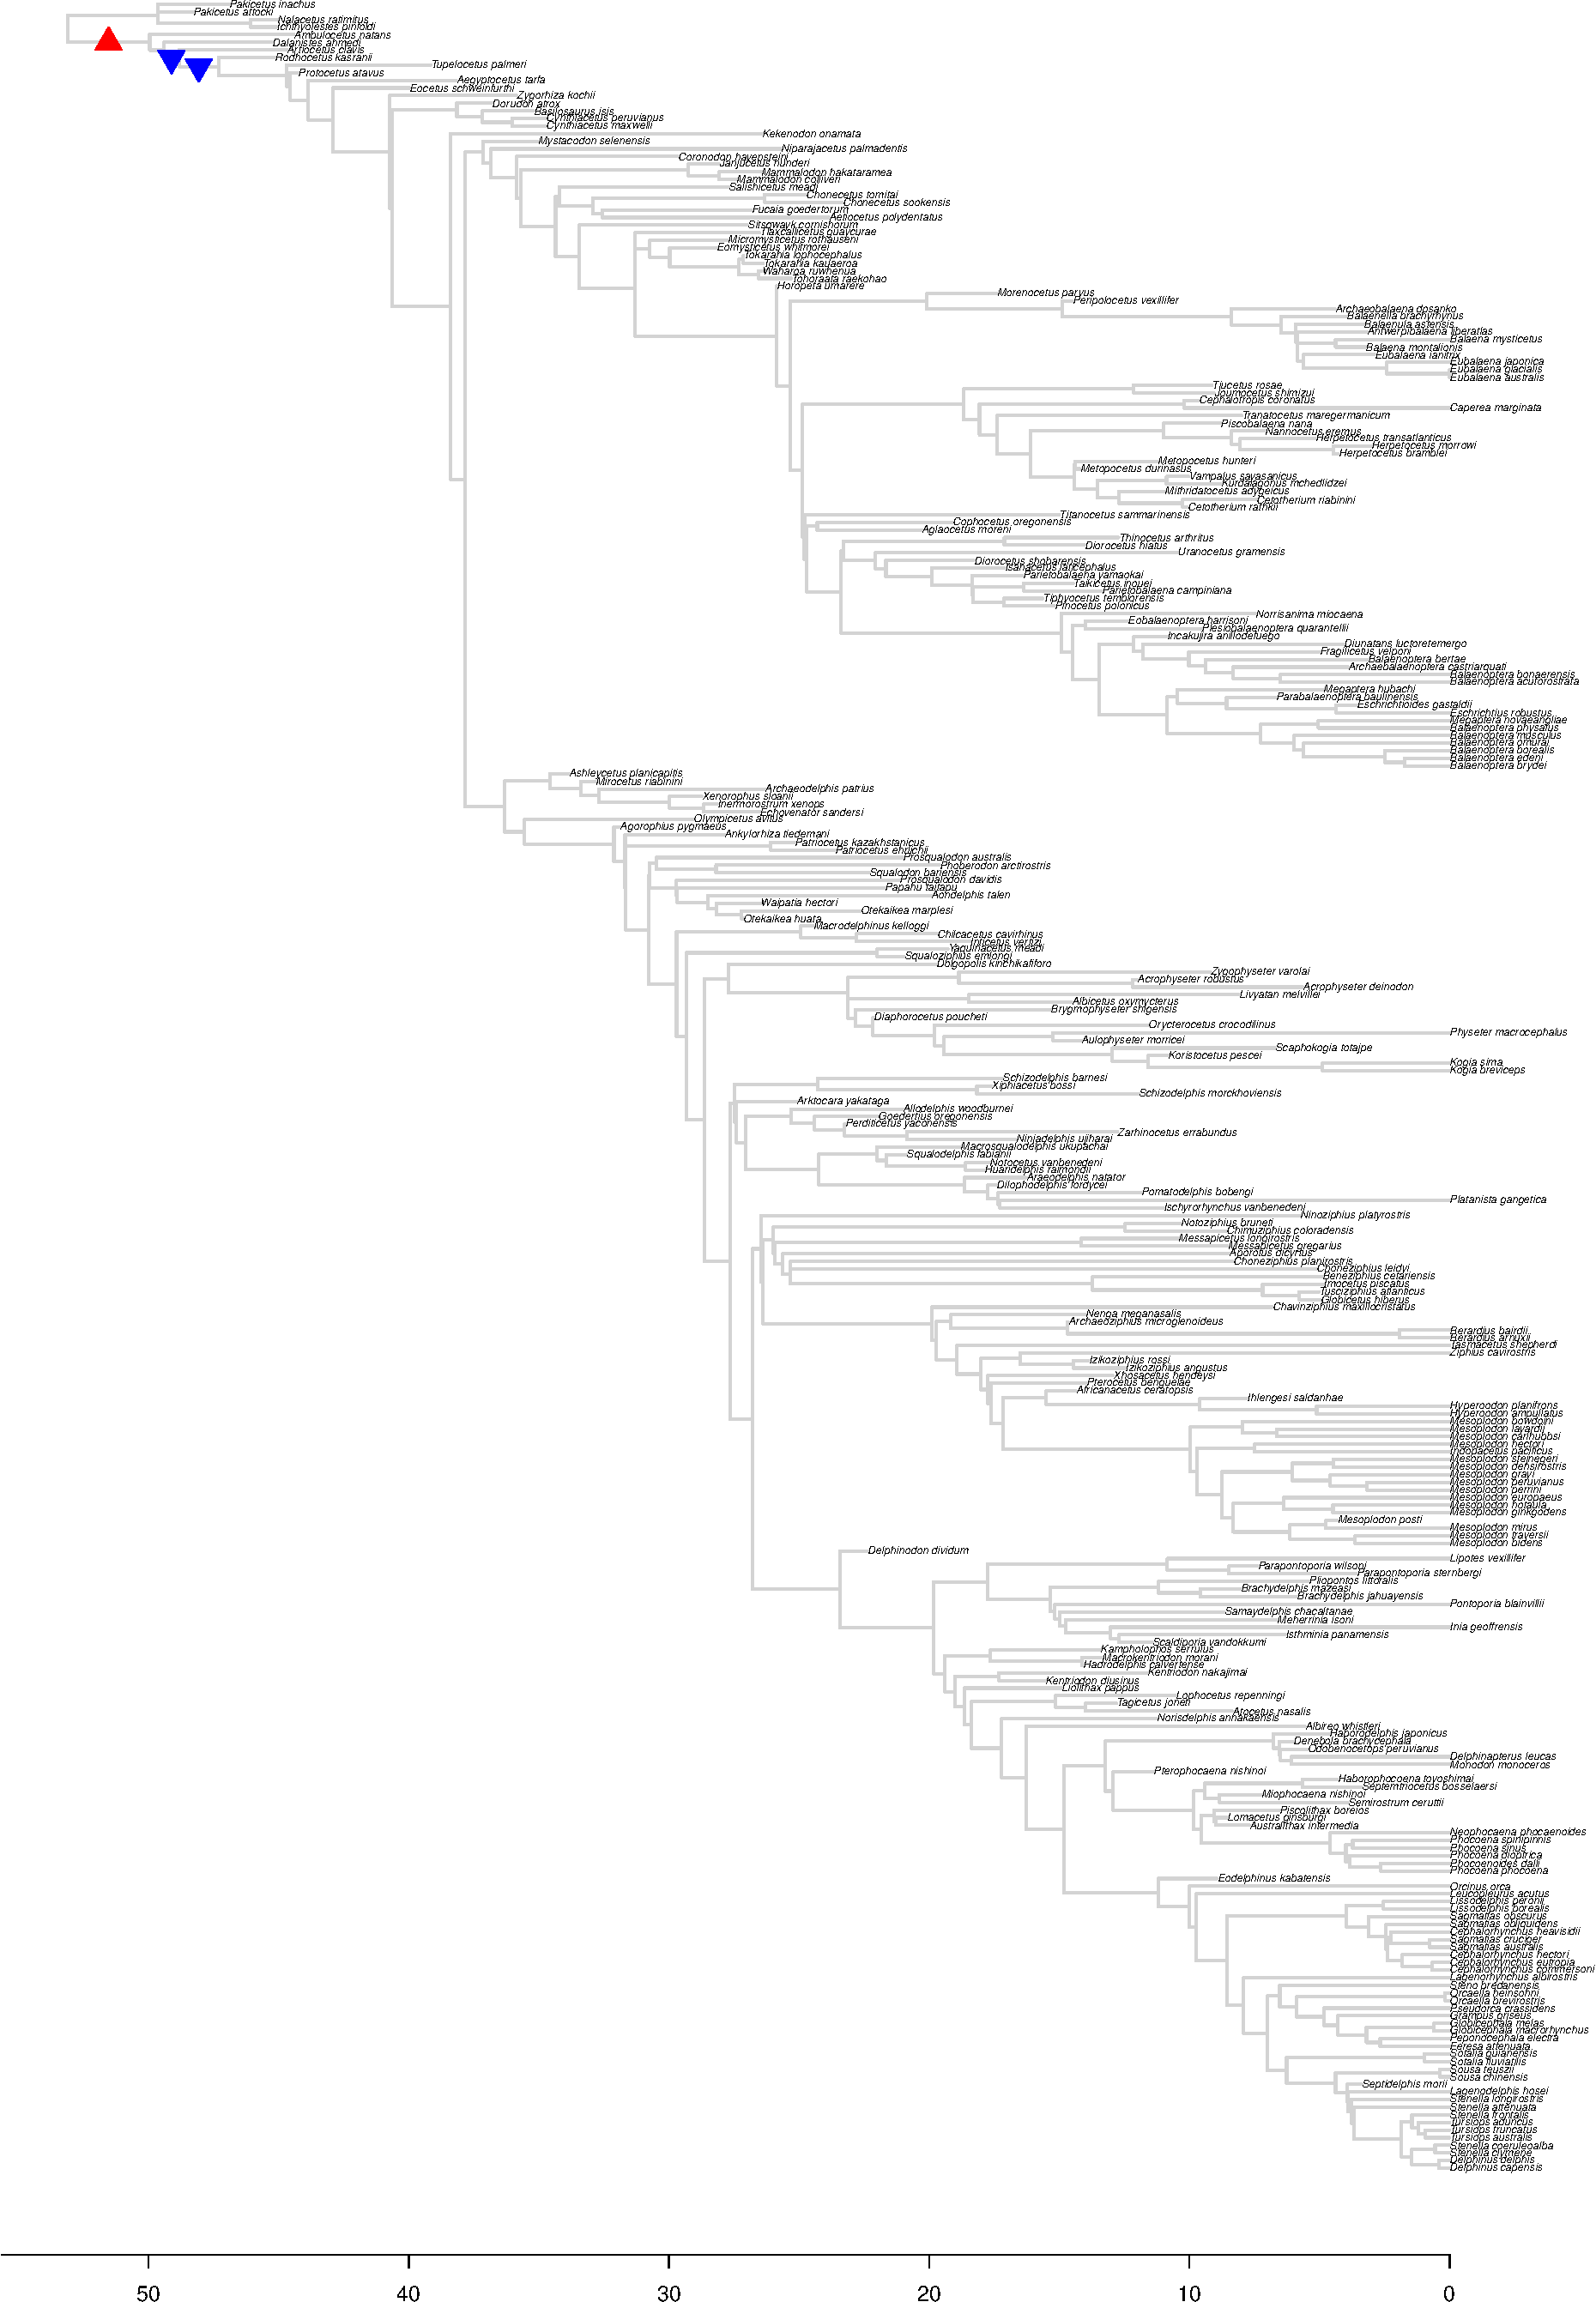
\includegraphics[width=0.8\textwidth]{img/plots-full-k5-1.pdf}
\caption{Results for \textit{bayou} fit for the \textit{Full} tree, excluding taxa on zero-length branches, setting the average number of shifts in the prior distribution ($\lambda$) to 5. The triangles represent the position and direction of the shifts with posterior probability higher than 0.1, with upward triangles (in red) indicating increases in $\theta$, and downward triangles (in blue) indicating decreases in $\theta$.}
\label{fig:full-k5-nzlb}
\end{figure}

\newpage

\begin{figure}[H]
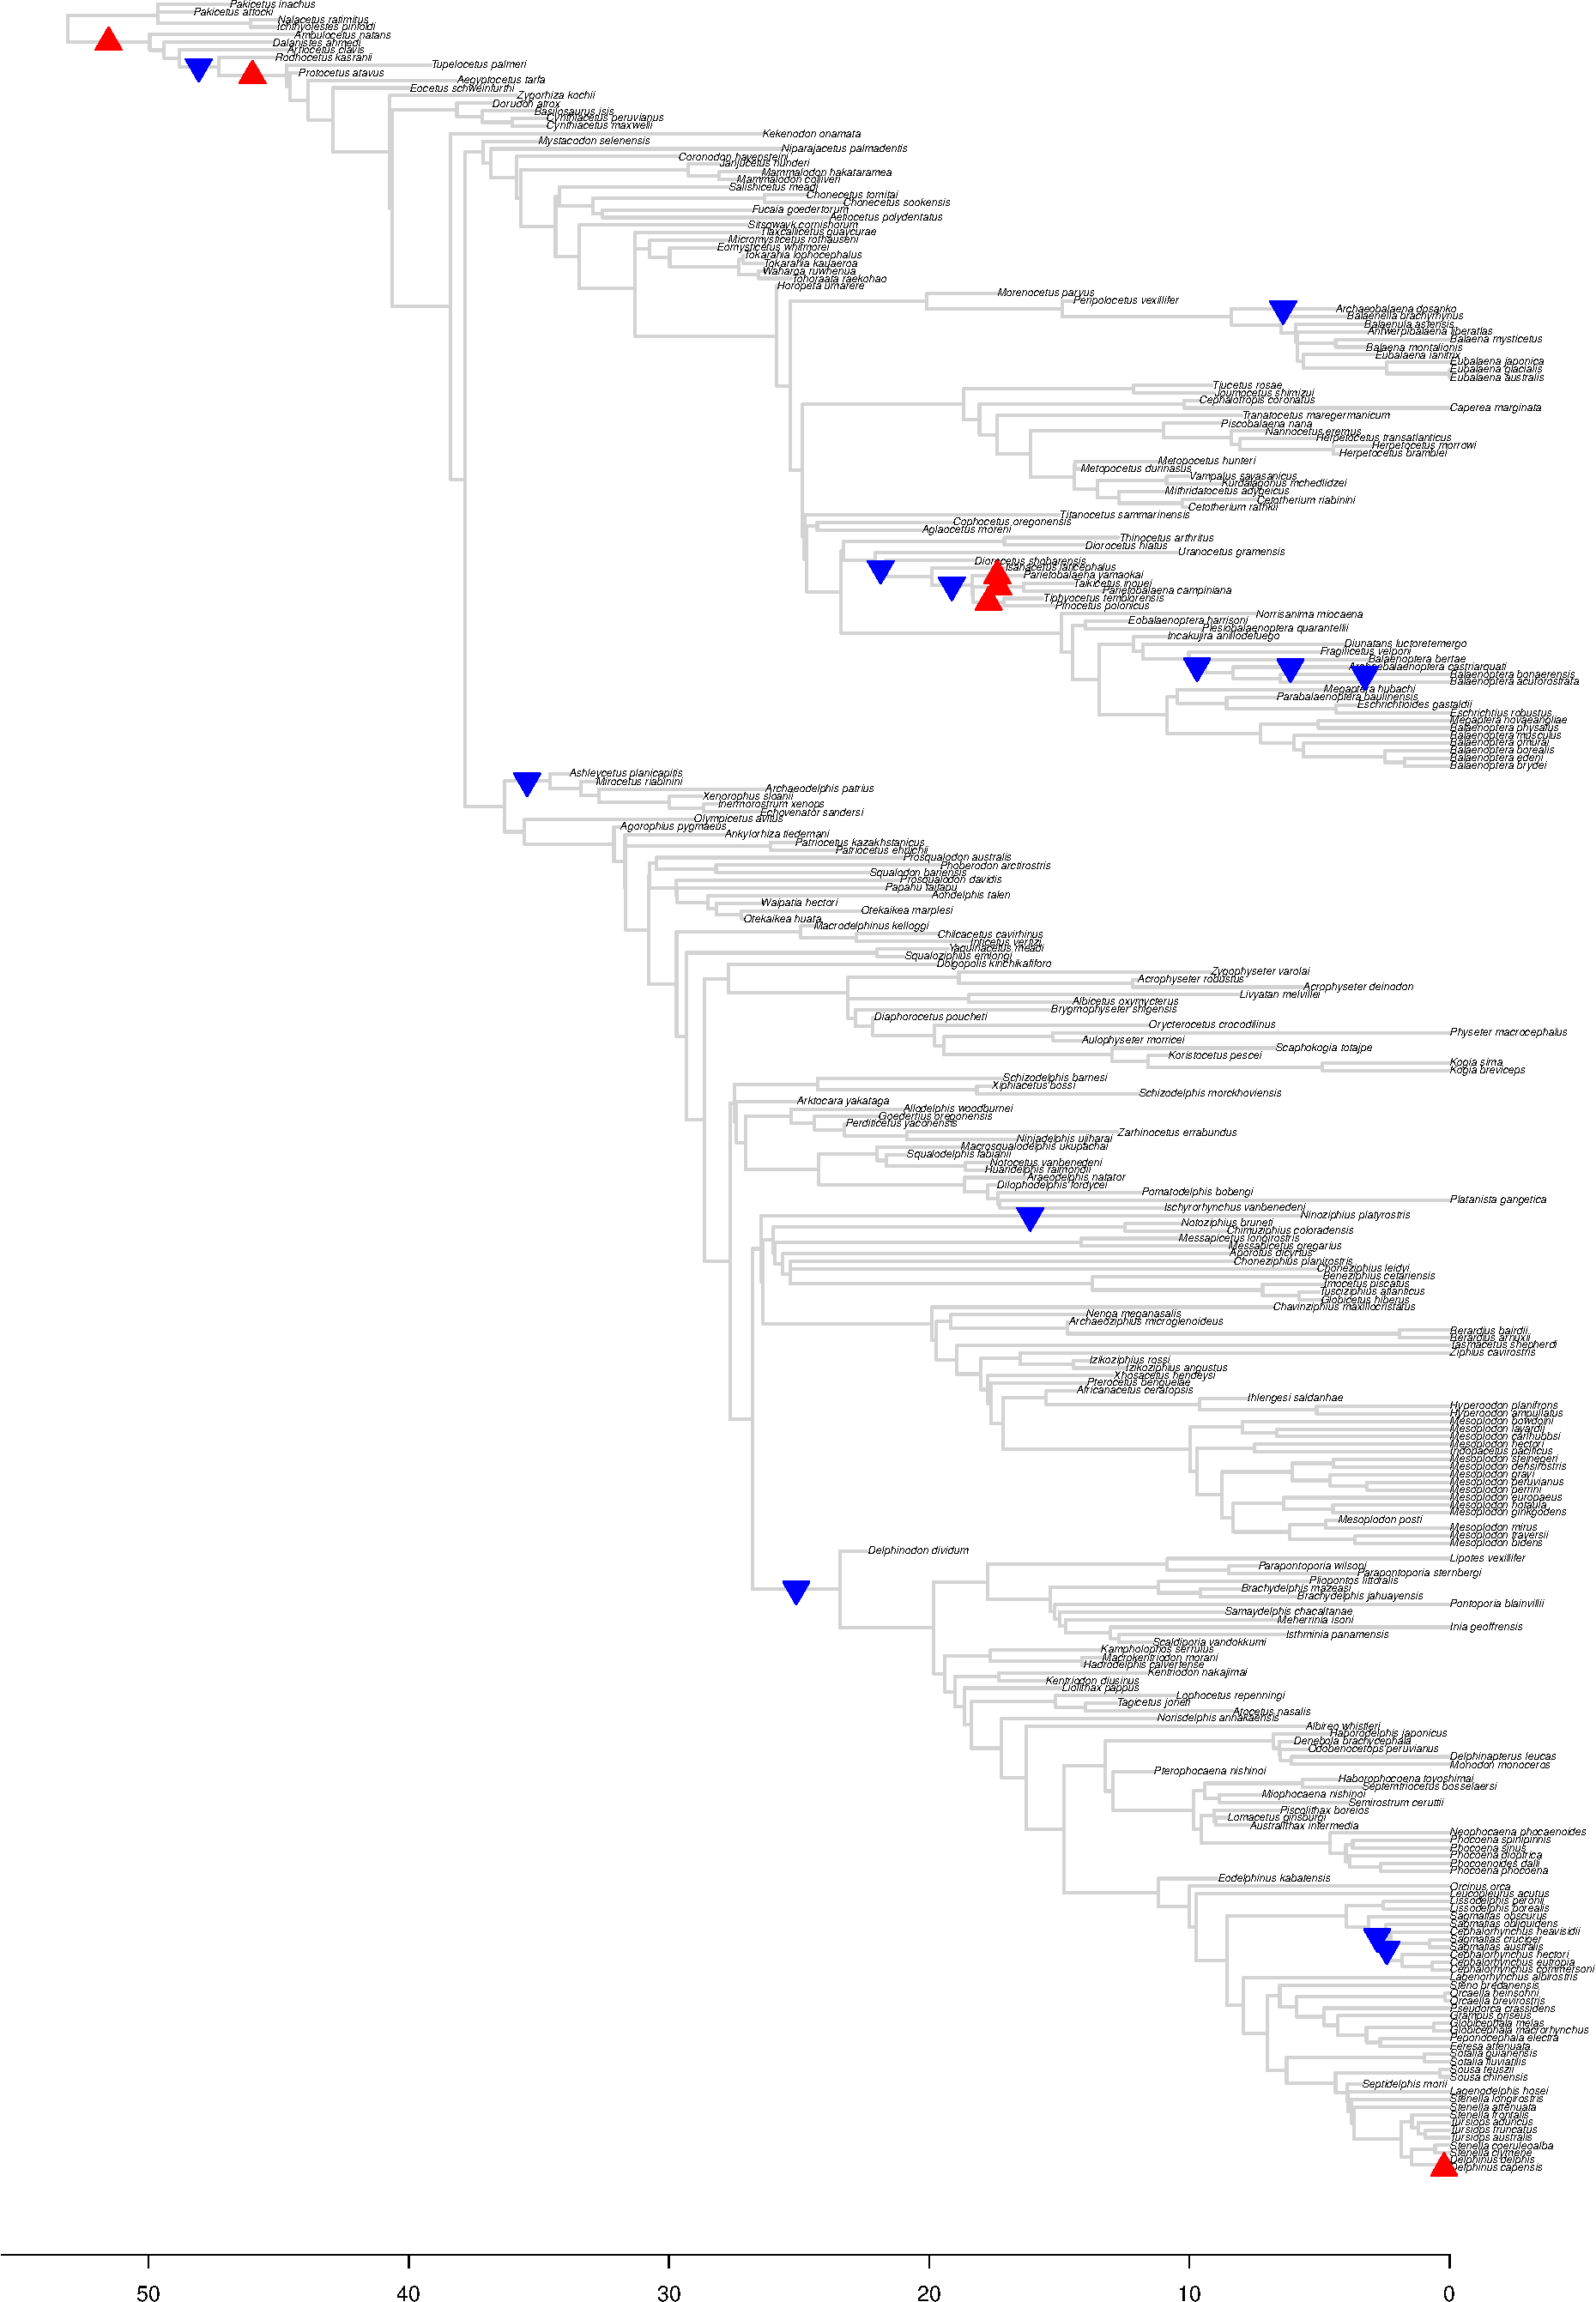
\includegraphics[width=0.9\textwidth]{img/plots-full-k15-1.pdf}
\caption{Results for \textit{bayou} fit for the \textit{Full} tree, excluding taxa on zero-length branches, setting the average number of shifts in the prior distribution ($\lambda$) to 15. The triangles represent the position and direction of the shifts with posterior probability higher than 0.1, with upward triangles (in red) indicating increases in $\theta$, and downward triangles (in blue) indicating decreases in $\theta$.}
\label{fig:full-k15-nzlb}
\end{figure}

\newpage

\begin{figure}[H]
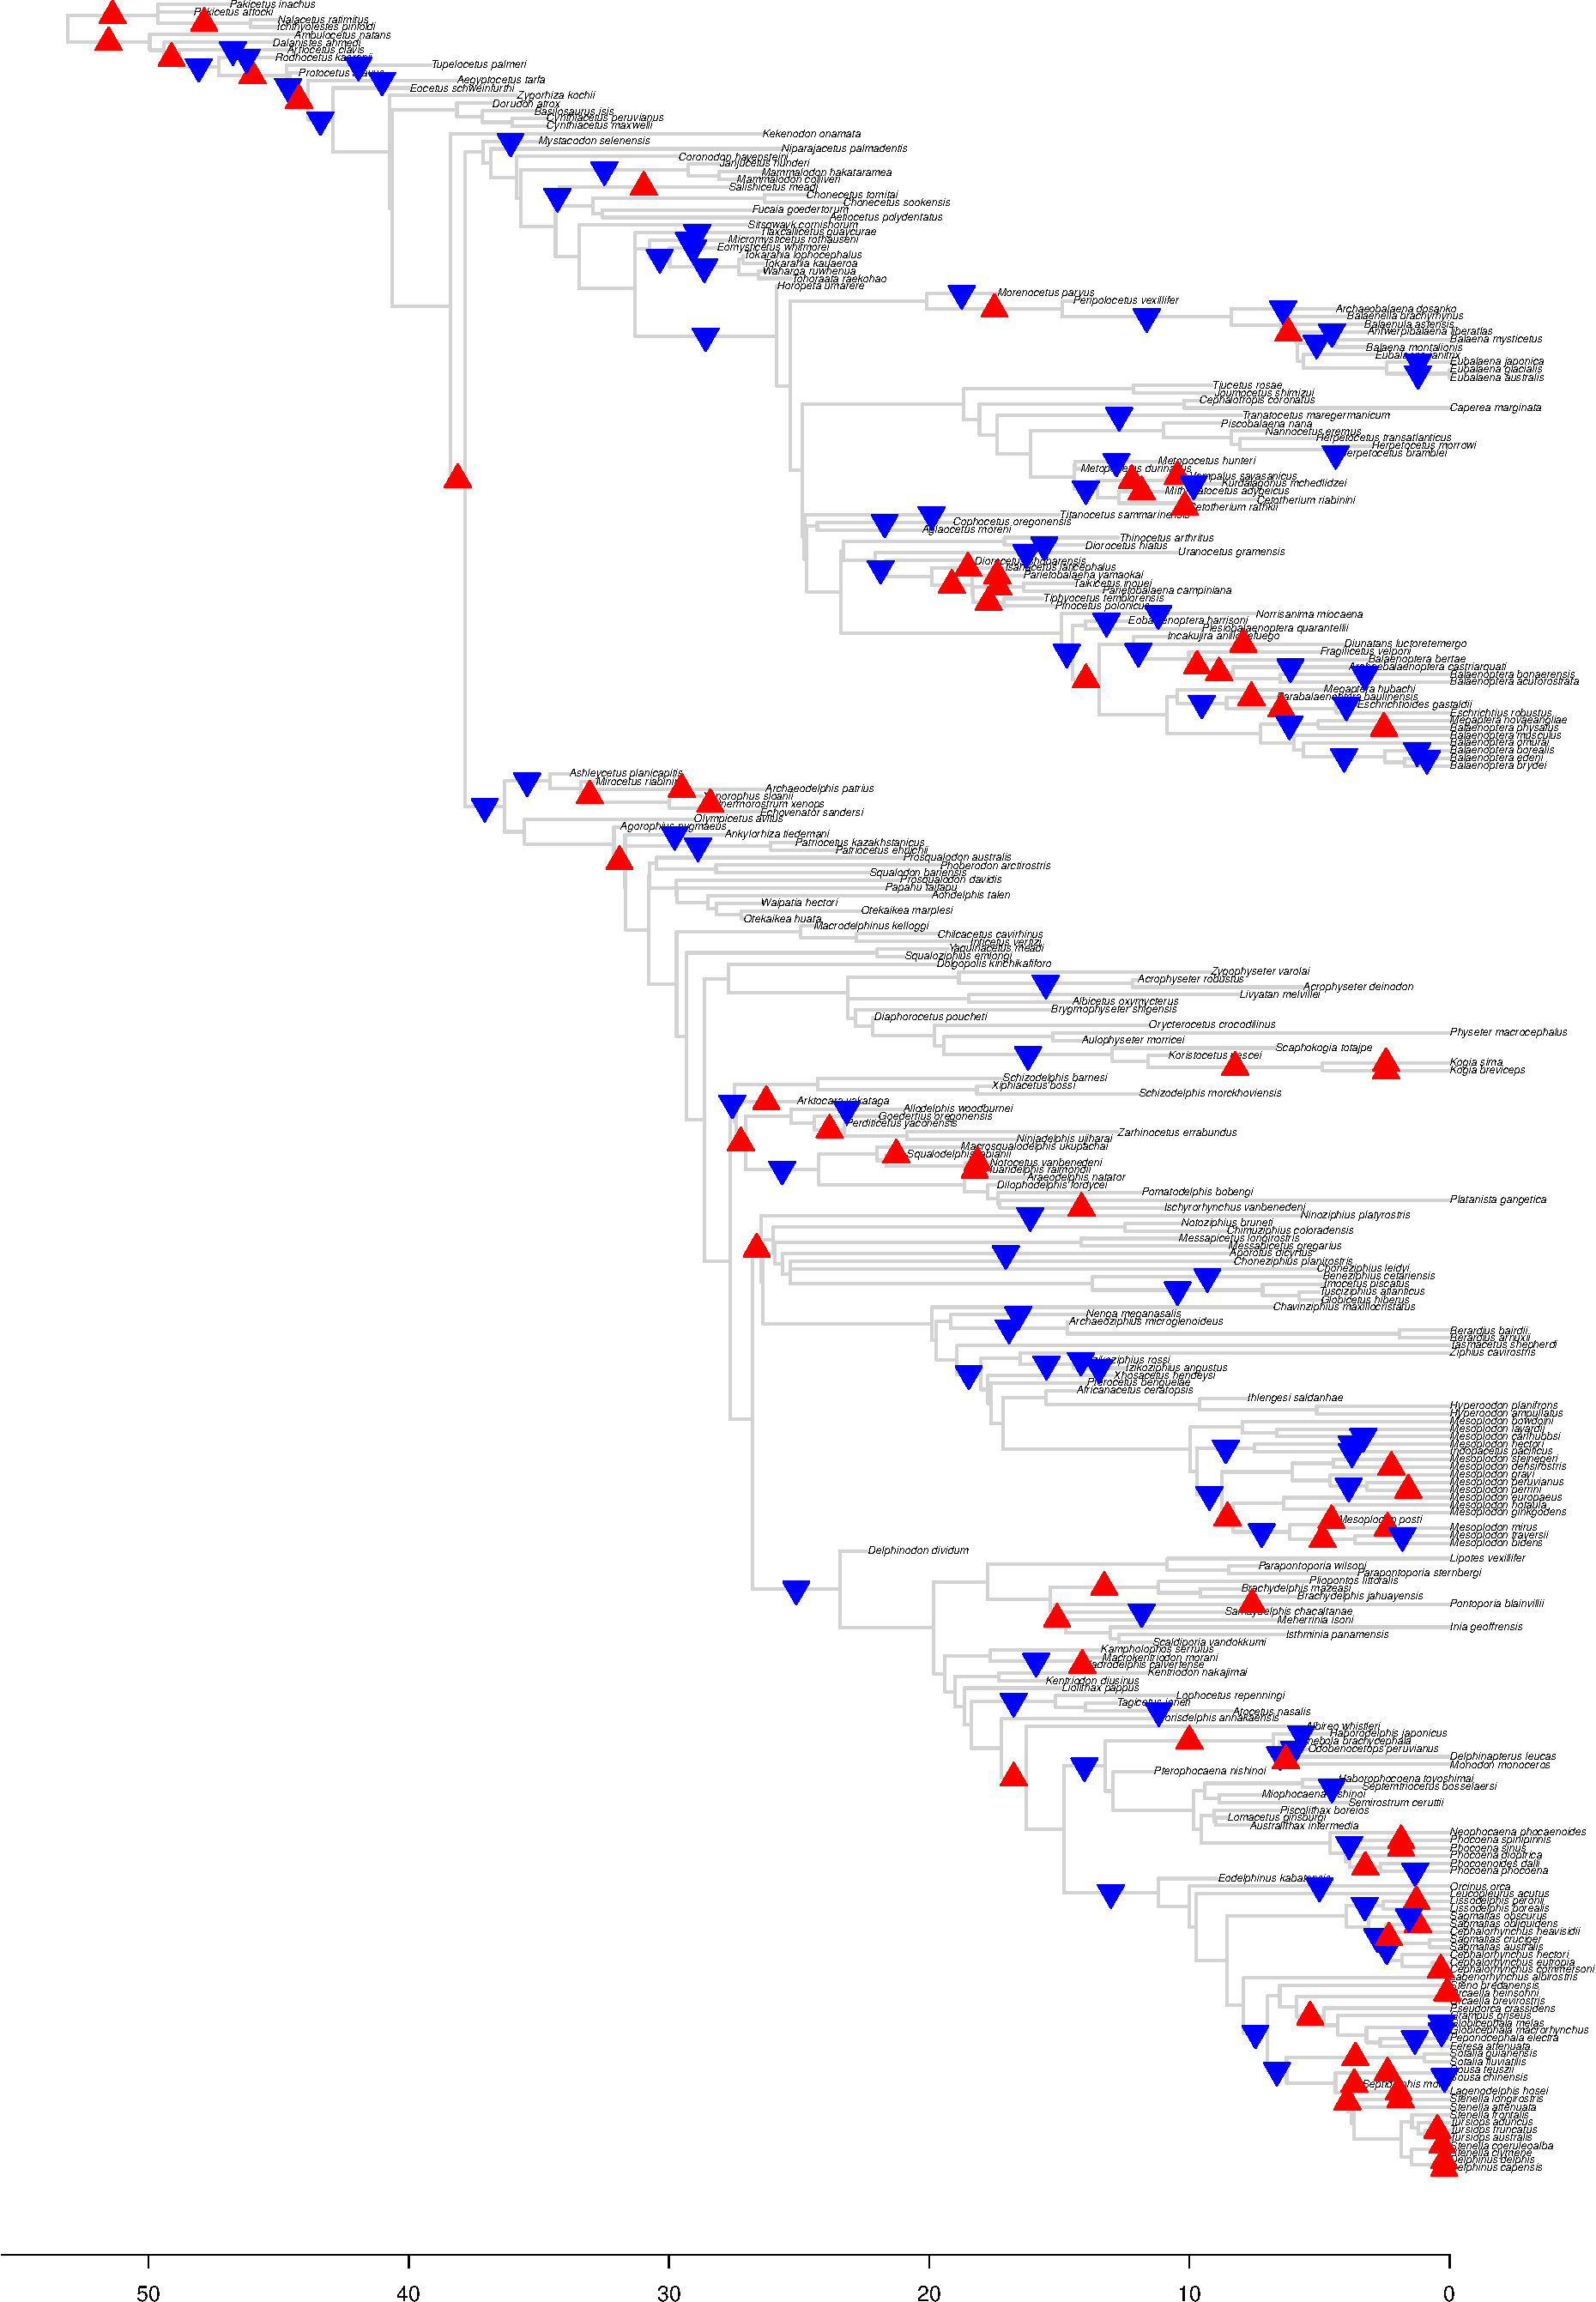
\includegraphics[width=0.9\textwidth]{img/plots-full-k50-1.pdf}
\caption{Results for \textit{bayou} fit for the \textit{Full} tree, excluding taxa on zero-length branches, setting the average number of shifts in the prior distribution ($\lambda$) to 50. The triangles represent the position and direction of the shifts with posterior probability higher than 0.1, with upward triangles (in red) indicating increases in $\theta$, and downward triangles (in blue) indicating decreases in $\theta$.}
\label{fig:full-k50-nzlb}
\end{figure}

\newpage

\begin{figure}[H]
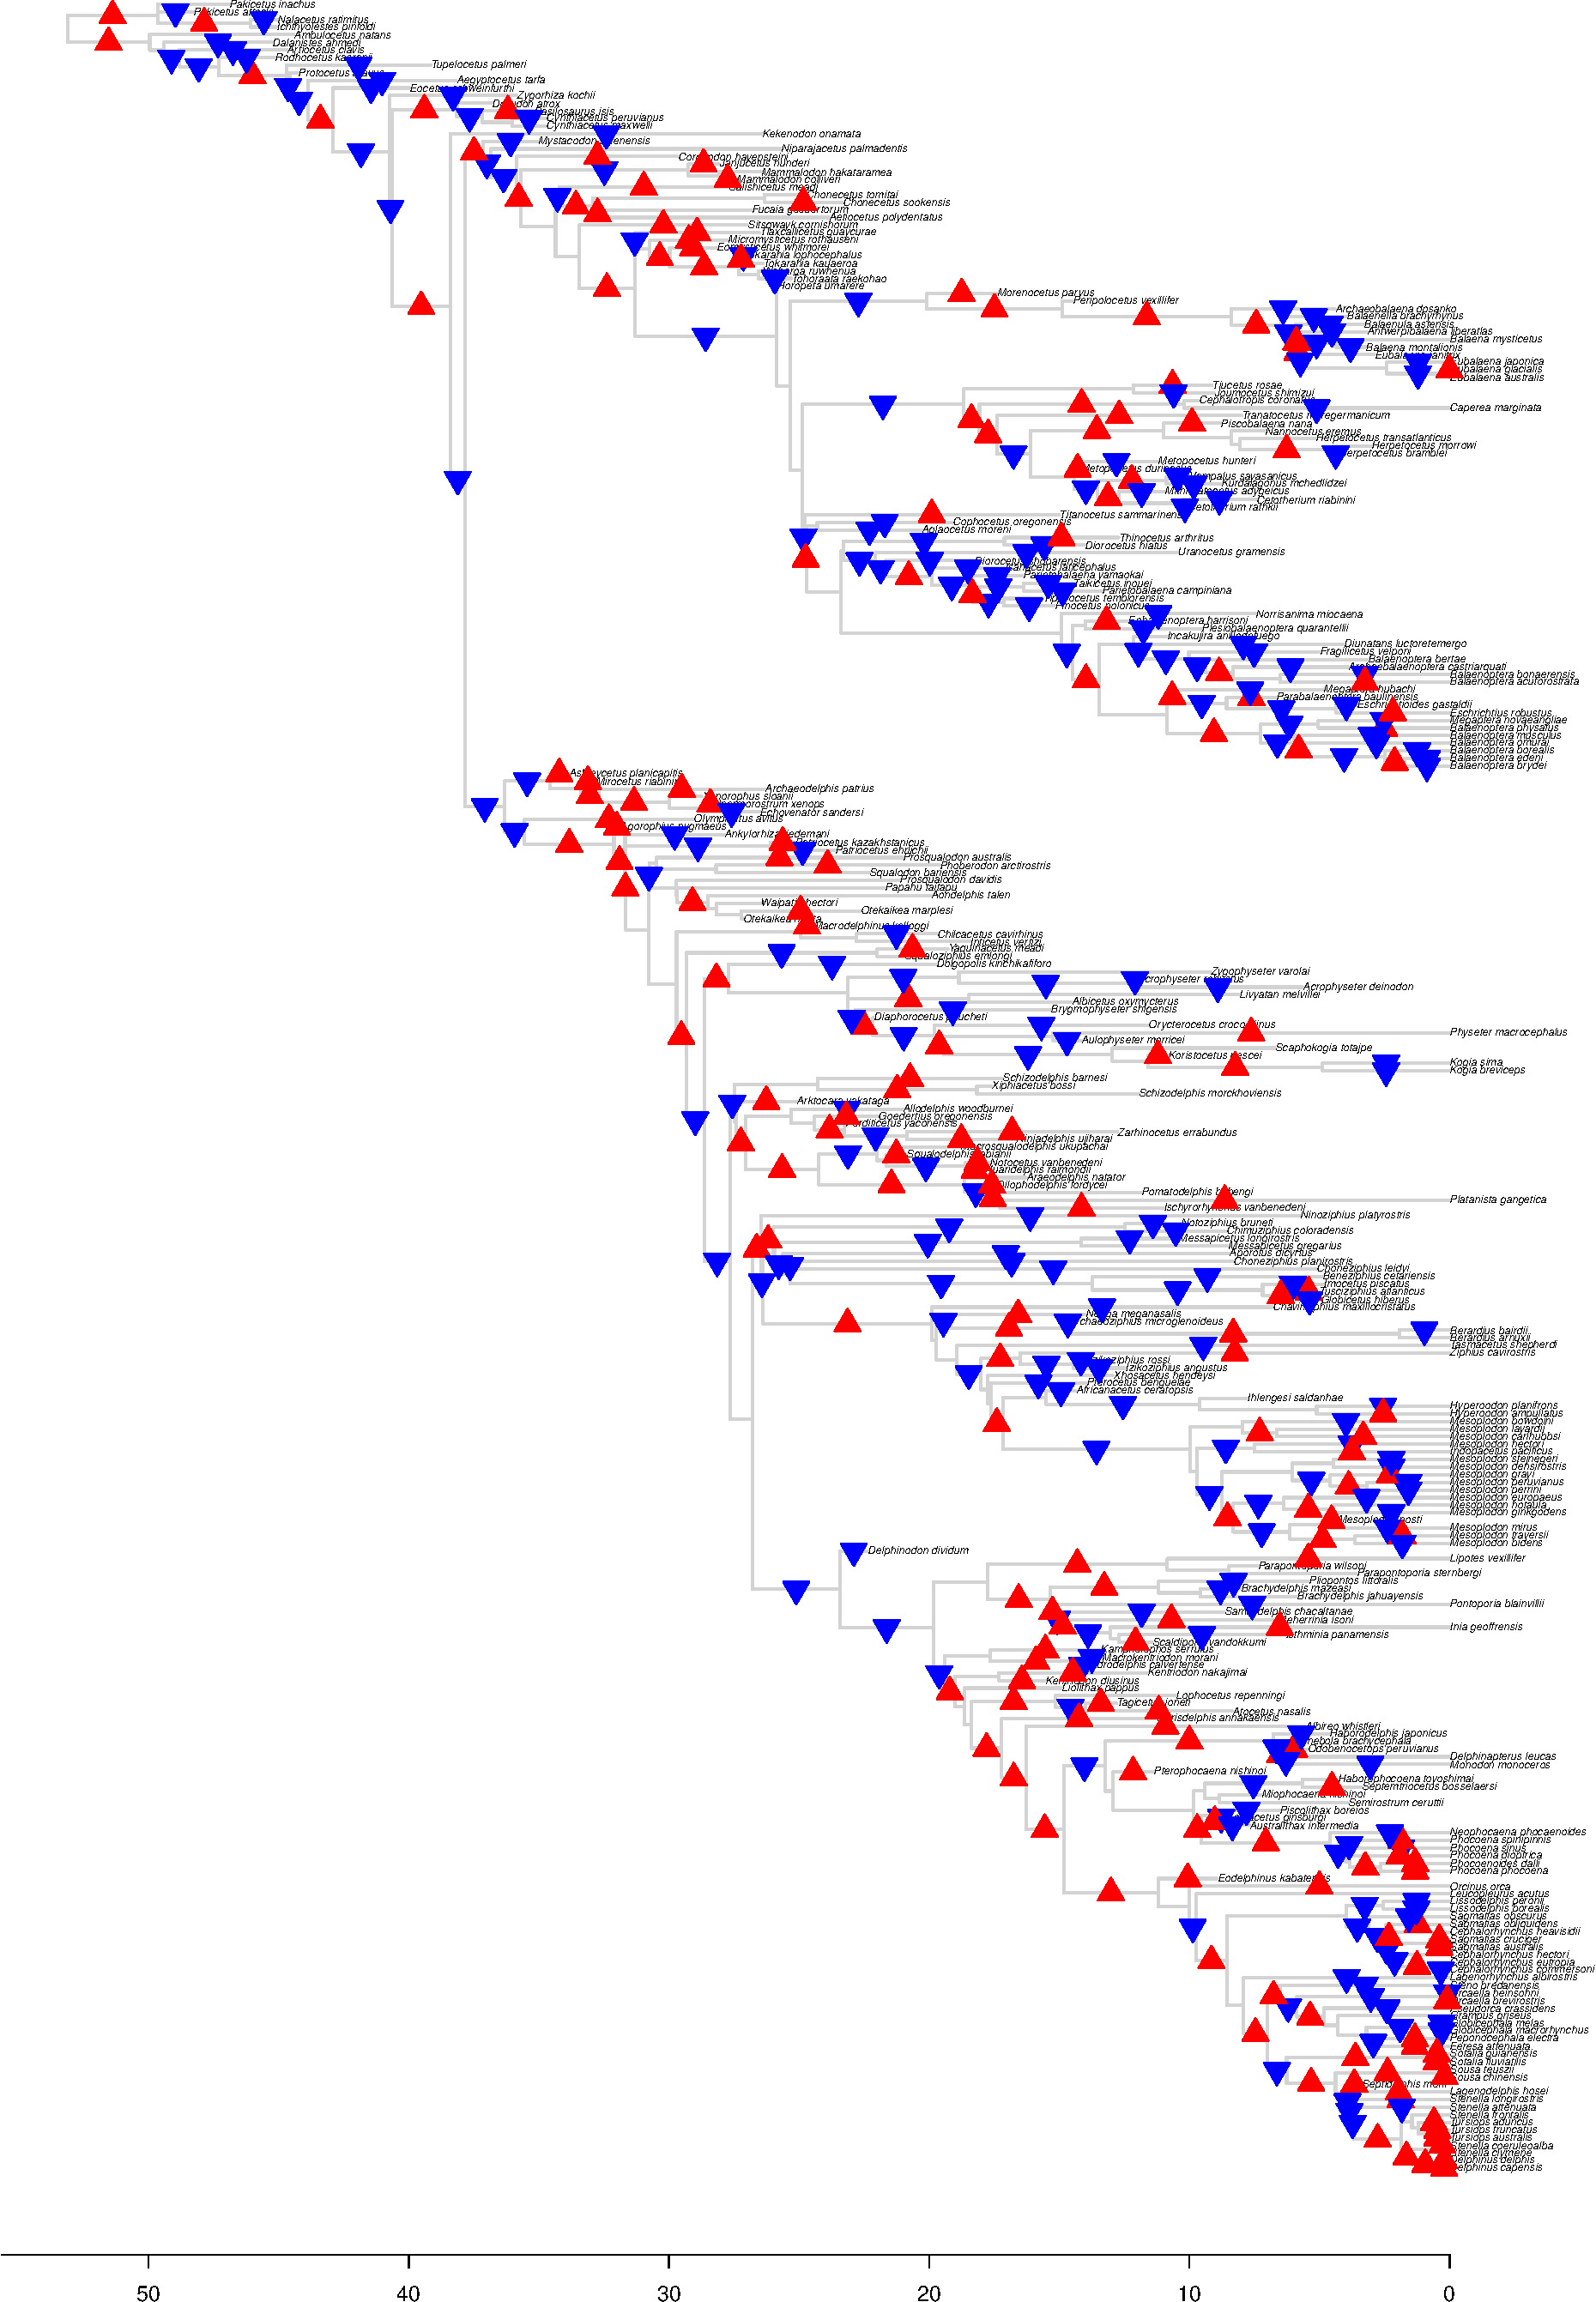
\includegraphics[width=0.9\textwidth]{img/plots-full-k250-1.pdf}
\caption{Results for \textit{bayou} fit for the \textit{Full} tree, excluding taxa on zero-length branches, setting the average number of shifts in the prior distribution ($\lambda$) to 250. The triangles represent the position and direction of the shifts with posterior probability higher than 0.1, with upward triangles (in red) indicating increases in $\theta$, and downward triangles (in blue) indicating decreases in $\theta$.}
\label{fig:full-k250-nzlb}
\end{figure}

\newpage

\begin{figure}[H]
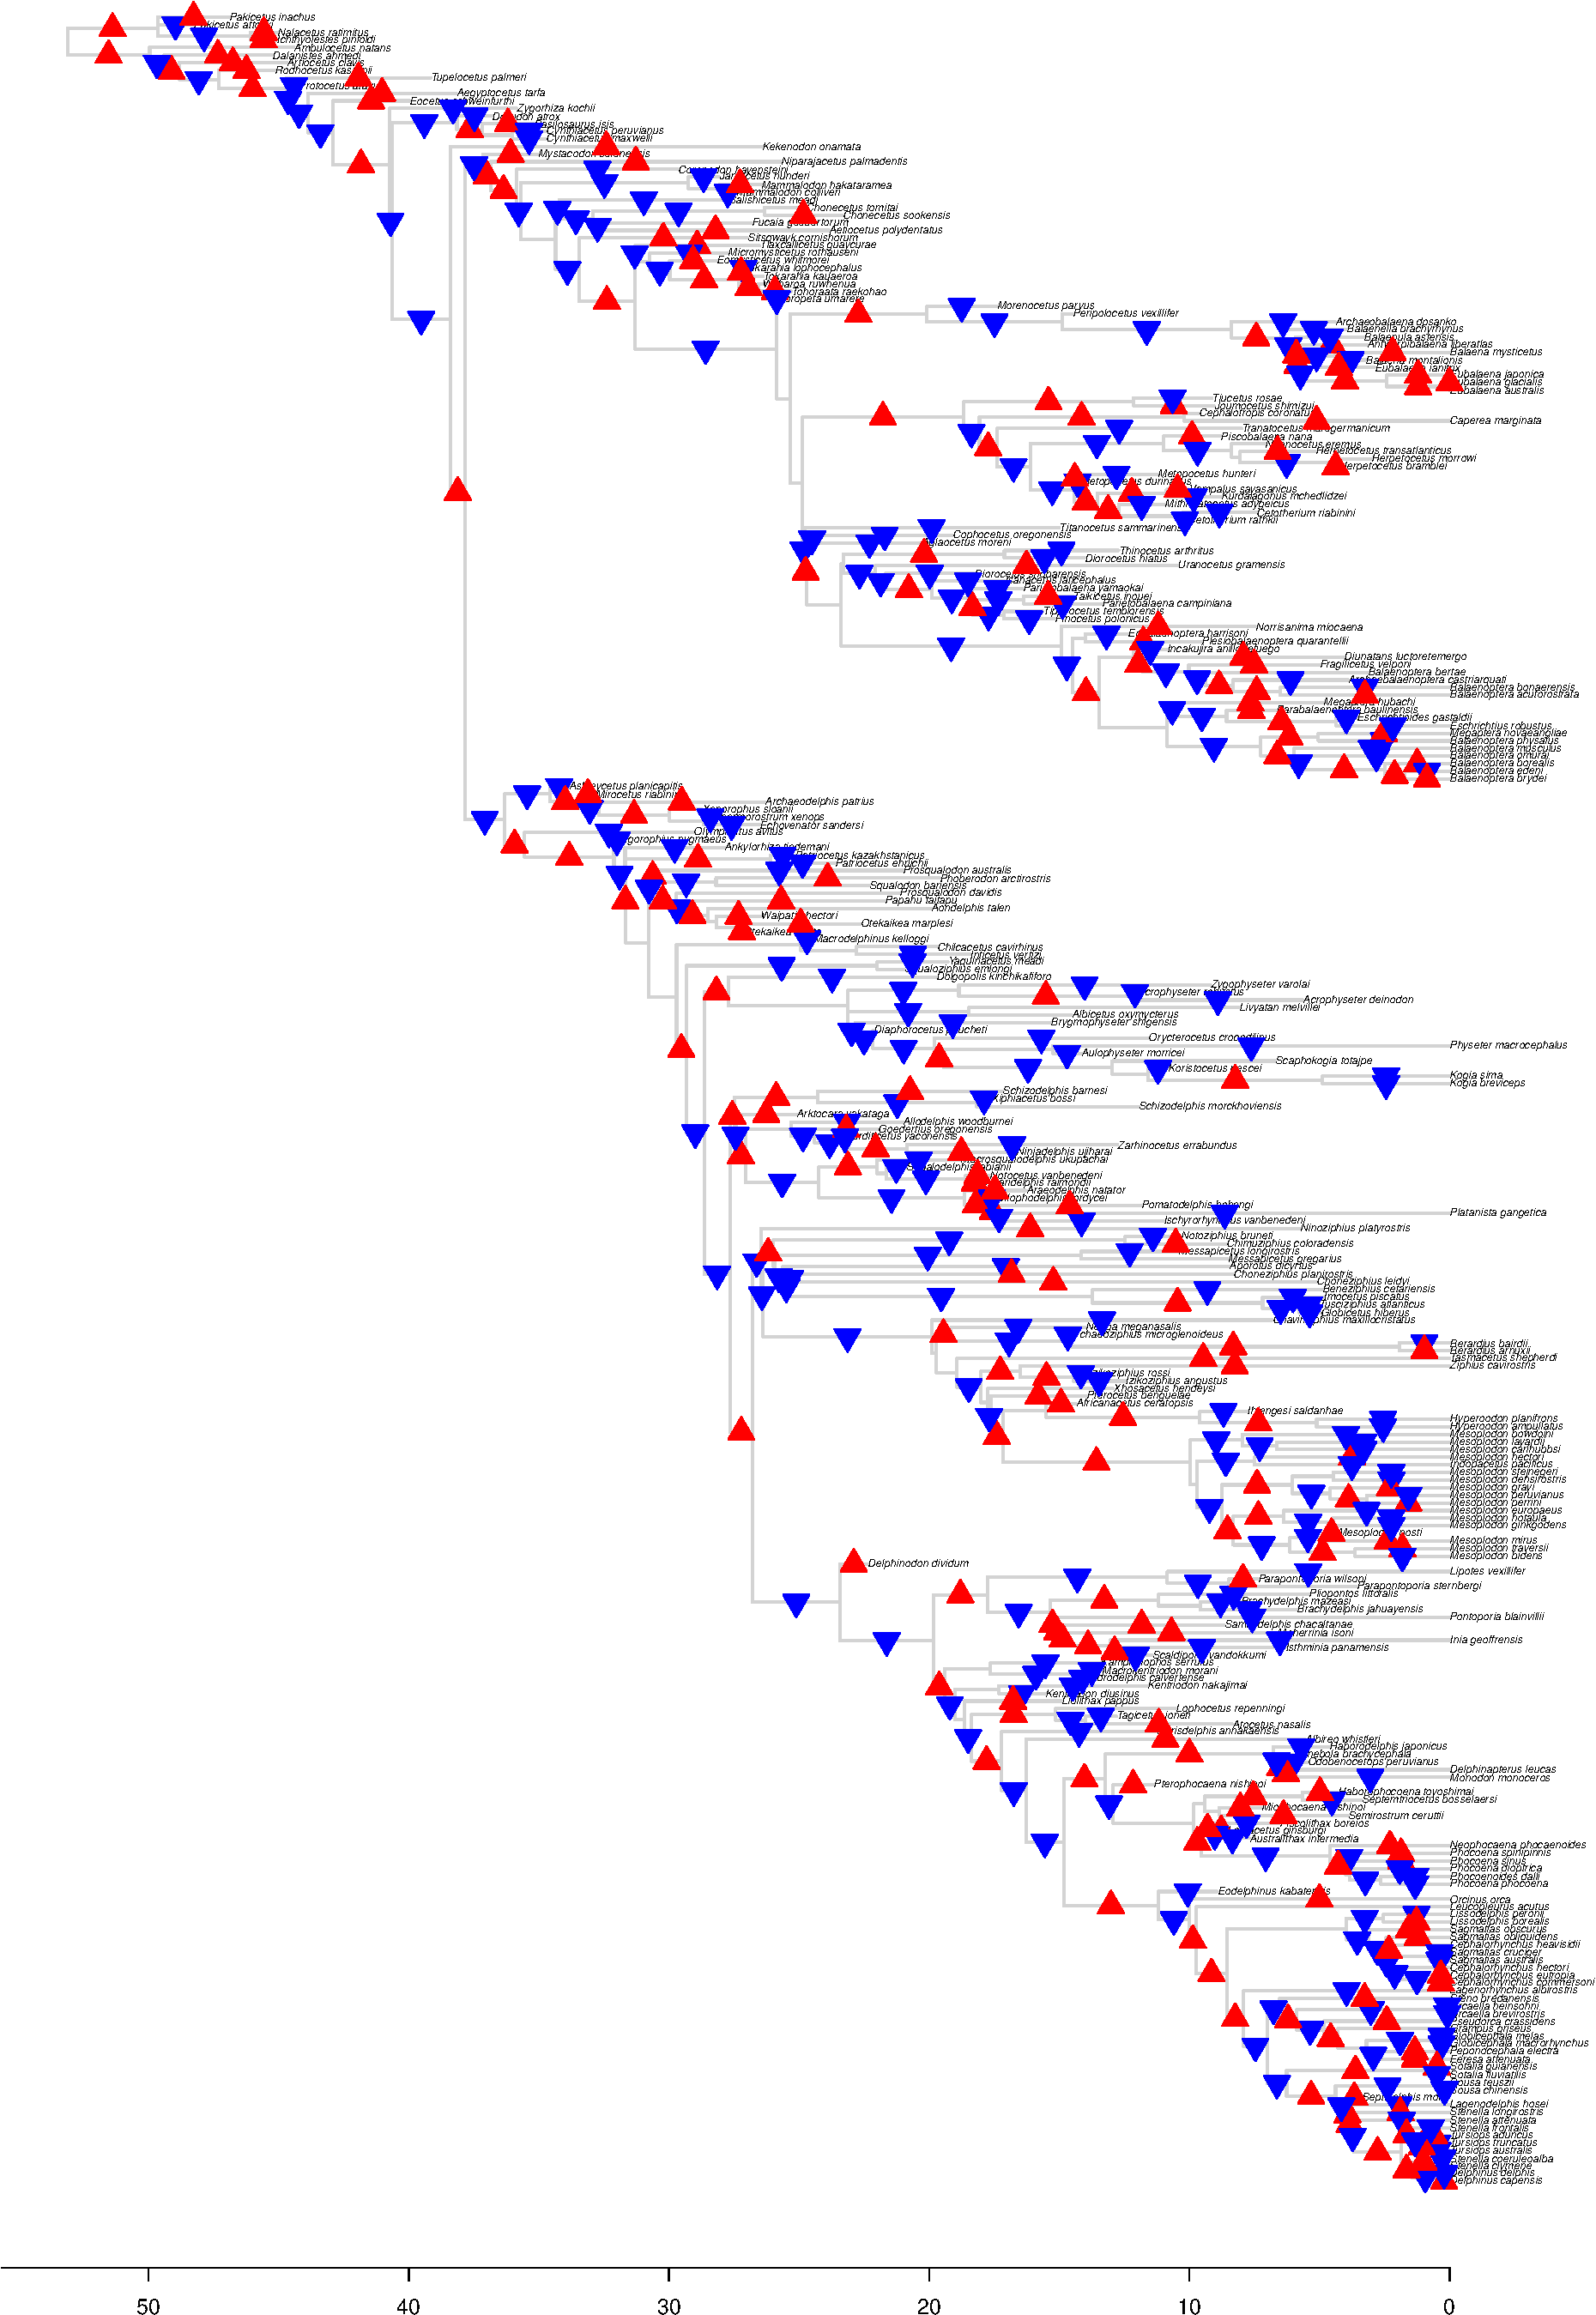
\includegraphics[width=0.9\textwidth]{img/plots-full-k500-1.pdf}
\caption{Results for \textit{bayou} fit for the \textit{Full} tree, excluding taxa on zero-length branches, setting the average number of shifts in the prior distribution ($\lambda$) to 500. The triangles represent the position and direction of the shifts with posterior probability higher than 0.1, with upward triangles (in red) indicating increases in $\theta$, and downward triangles (in blue) indicating decreases in $\theta$.}
\label{fig:full-k500-nzlb}
\end{figure}

%---------------------------------------------------------------------
\subsubsection{\textit{No Archaeoceti} tree}
%---------------------------------------------------------------------

\begin{figure}[H]
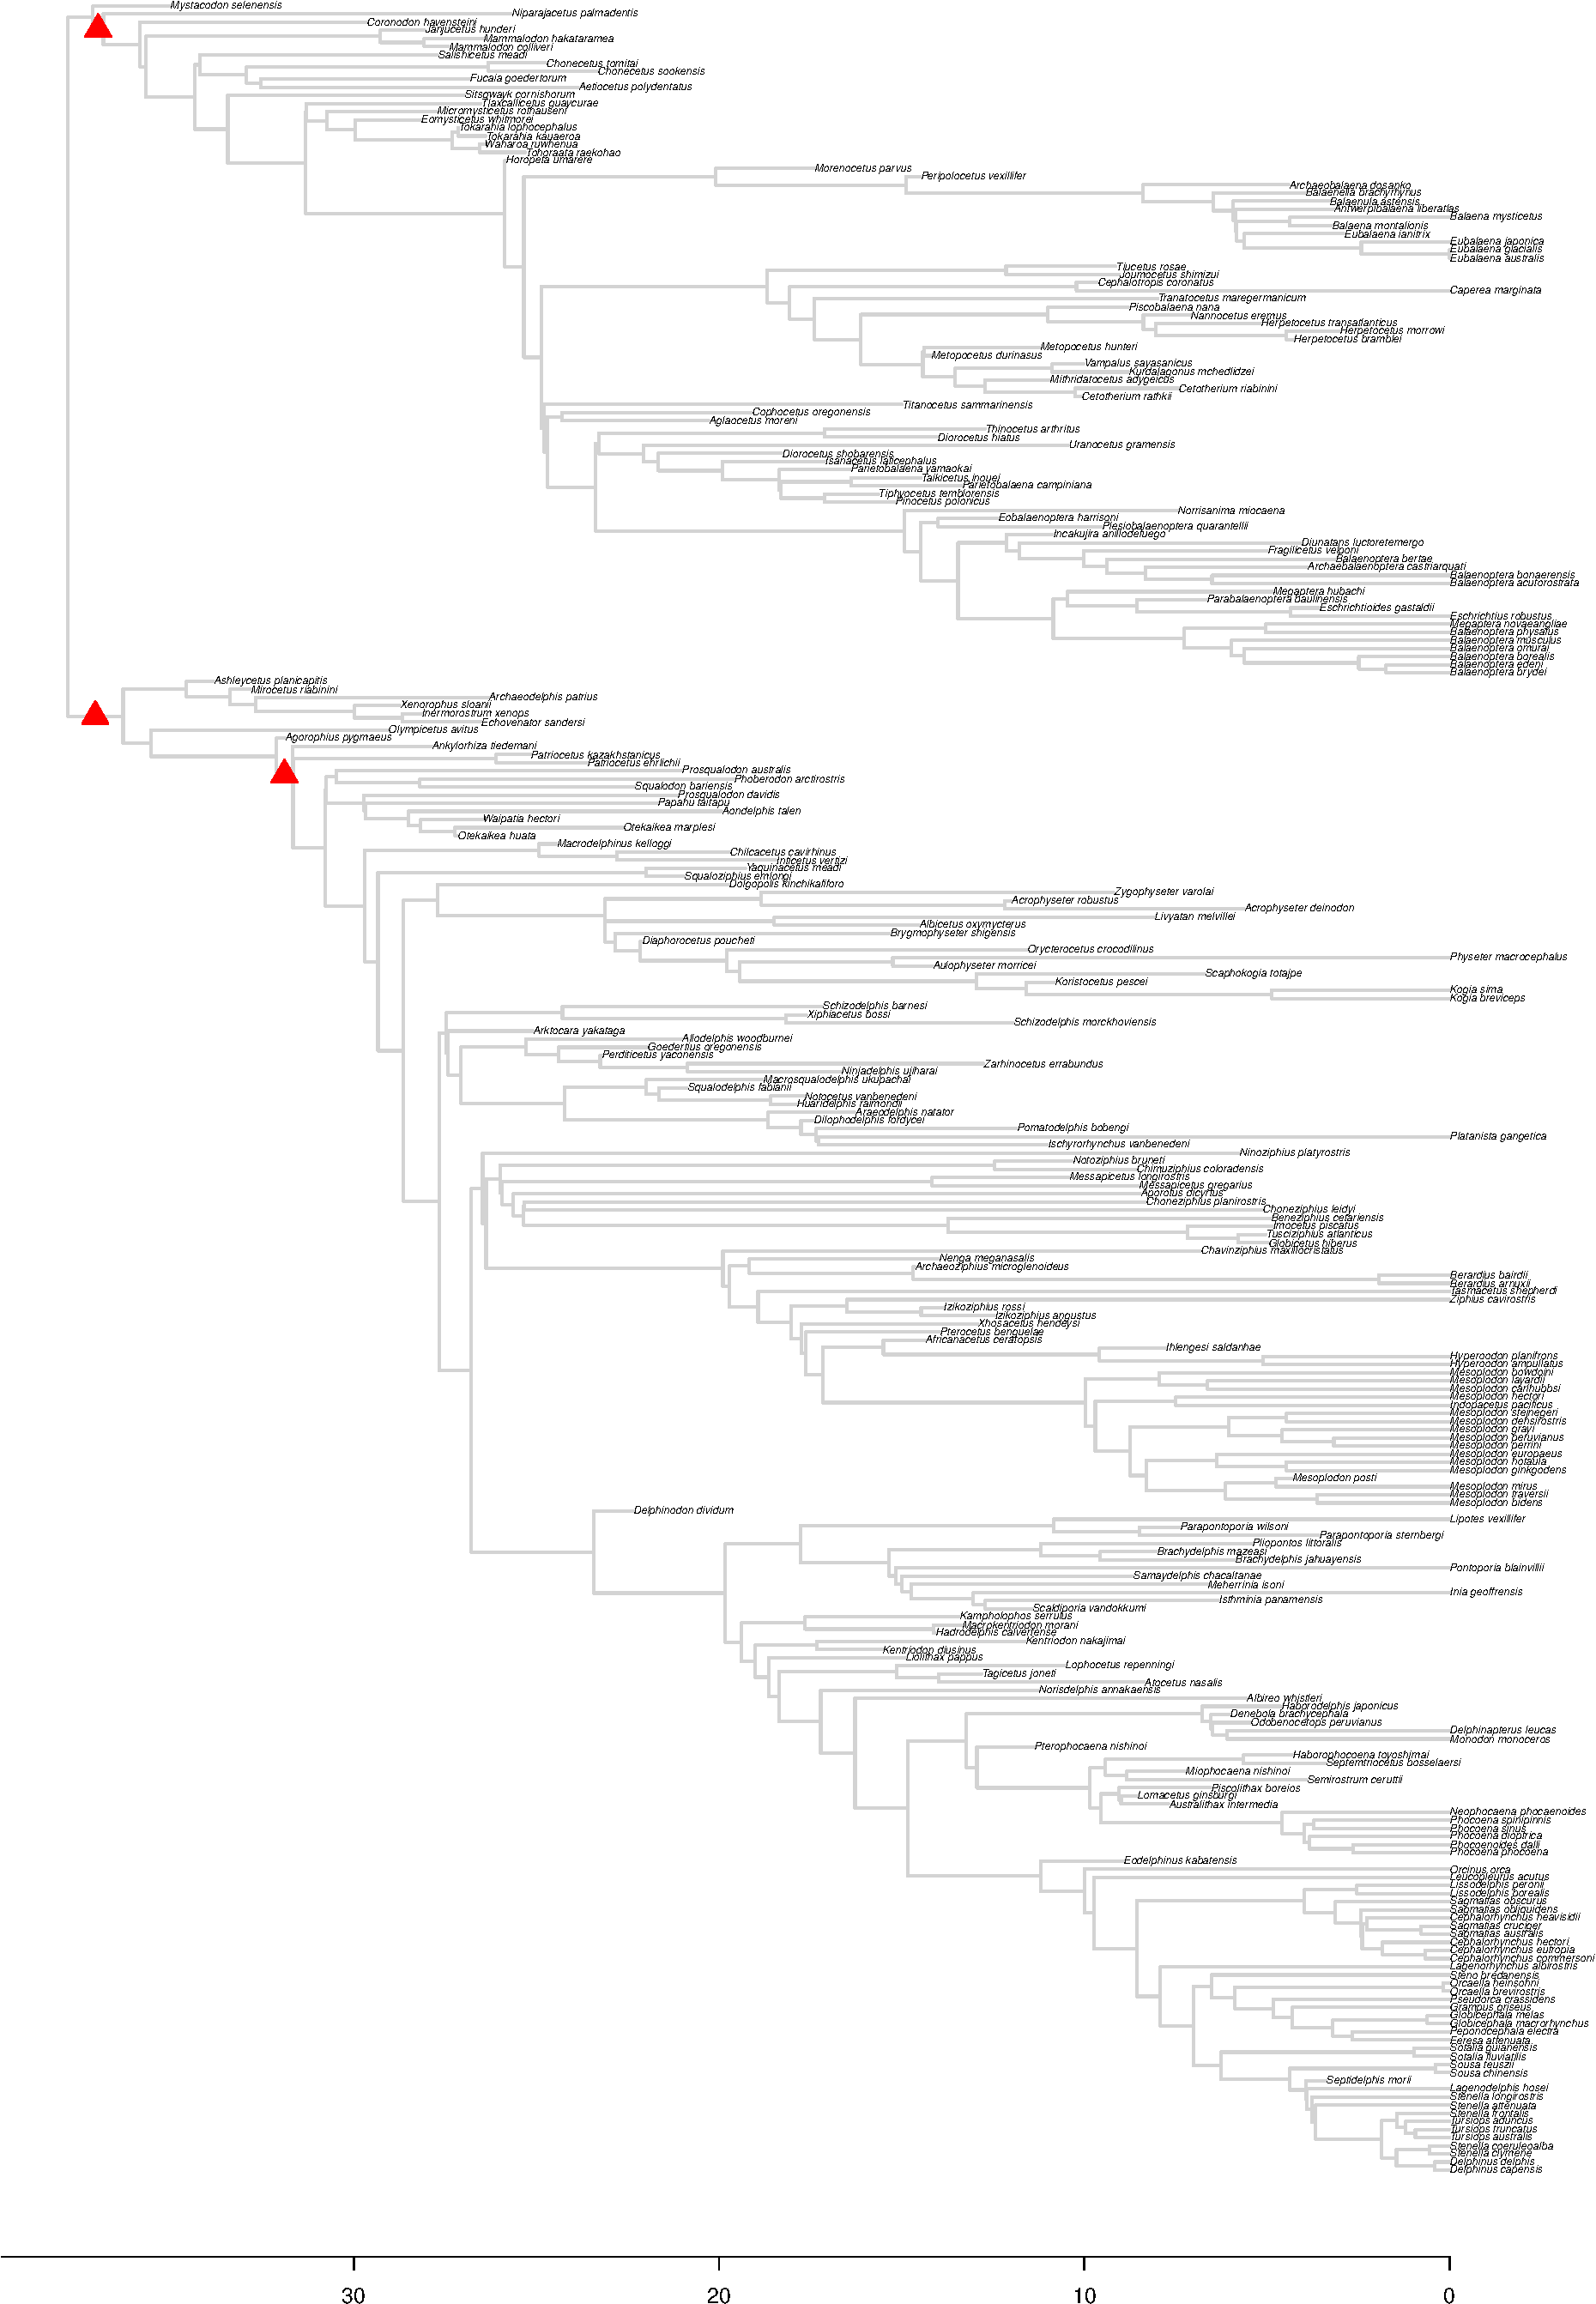
\includegraphics[width=0.9\textwidth]{img/plots-noarchaeo-k5-1.pdf}
\caption{Results for \textit{bayou} fit for the \textit{No Archaeoceti} tree, excluding taxa on zero-length branches, setting the average number of shifts in the prior distribution ($\lambda$) to 5. The triangles represent the position and direction of the shifts with posterior probability higher than 0.1, with upward triangles (in red) indicating increases in $\theta$, and downward triangles (in blue) indicating decreases in $\theta$.}
\label{fig:noarchaeo-k5-nzlb}
\end{figure}

\newpage

\begin{figure}[H]
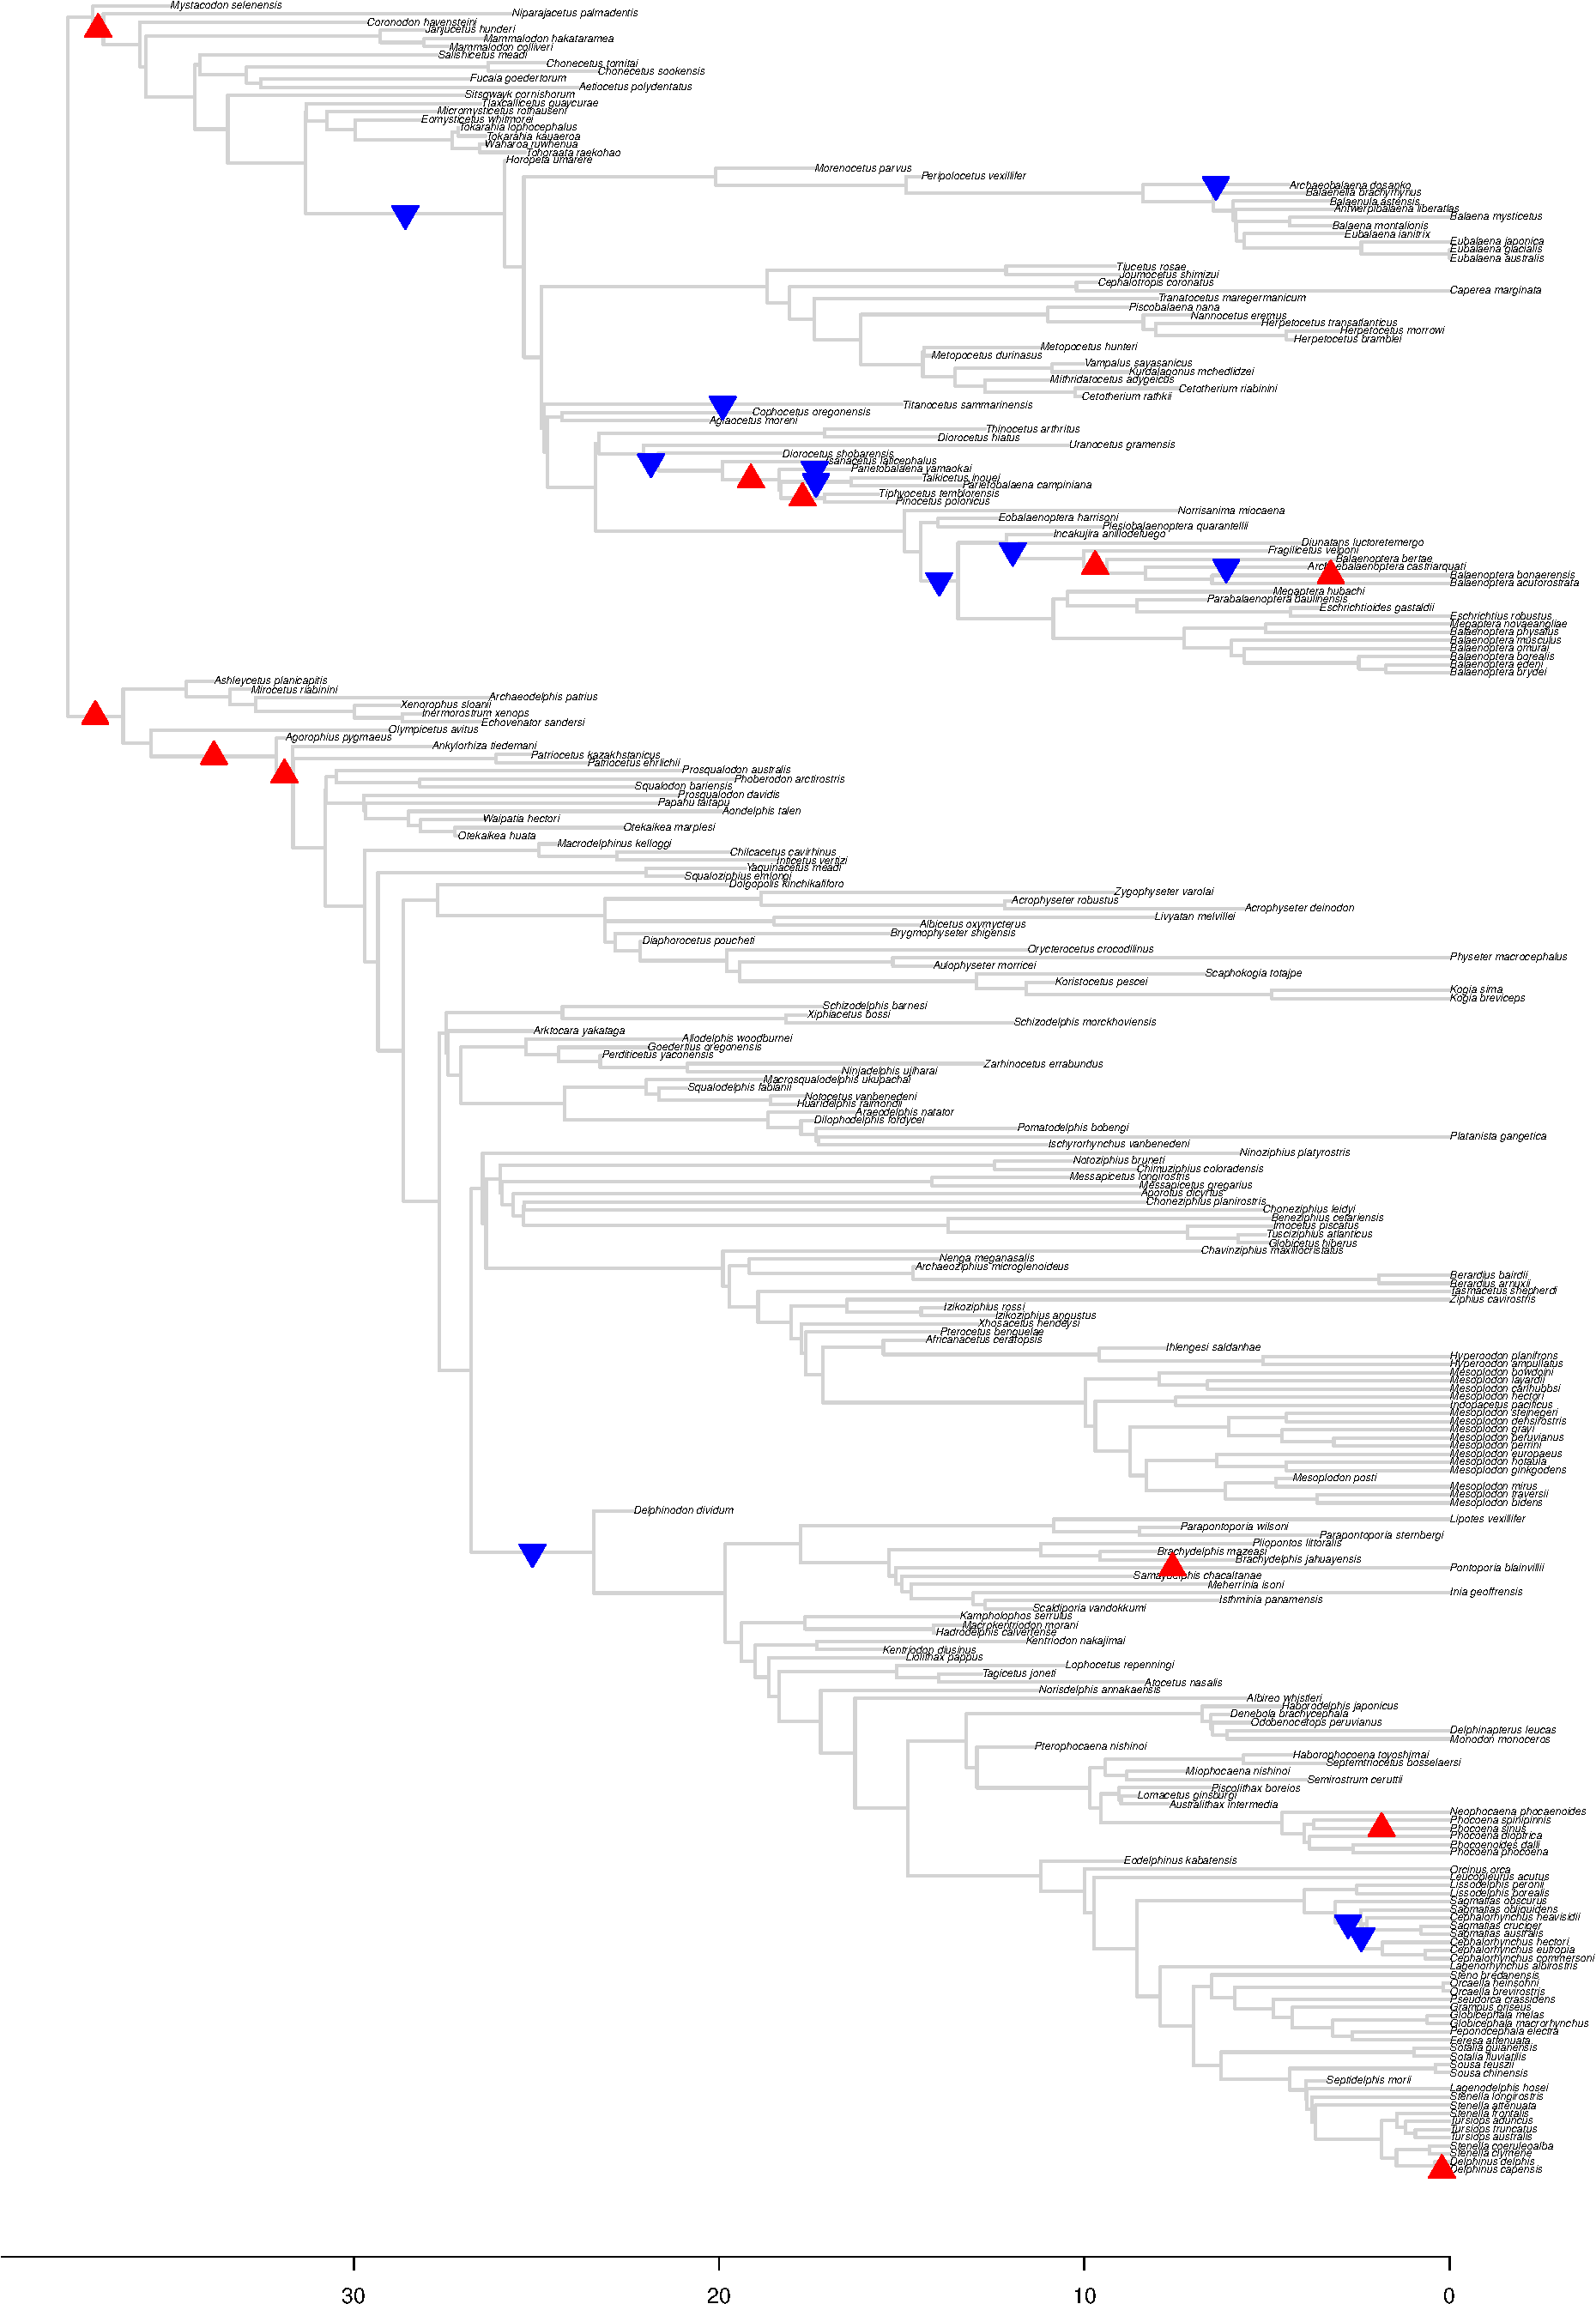
\includegraphics[width=0.9\textwidth]{img/plots-noarchaeo-k15-1.pdf}
\caption{Results for \textit{bayou} fit for the \textit{No Archaeoceti} tree, excluding taxa on zero-length branches, setting the average number of shifts in the prior distribution ($\lambda$) to 15. The triangles represent the position and direction of the shifts with posterior probability higher than 0.1, with upward triangles (in red) indicating increases in $\theta$, and downward triangles (in blue) indicating decreases in $\theta$.}
\label{fig:noarchaeo-k15-nzlb}
\end{figure}

\newpage

\begin{figure}[H]
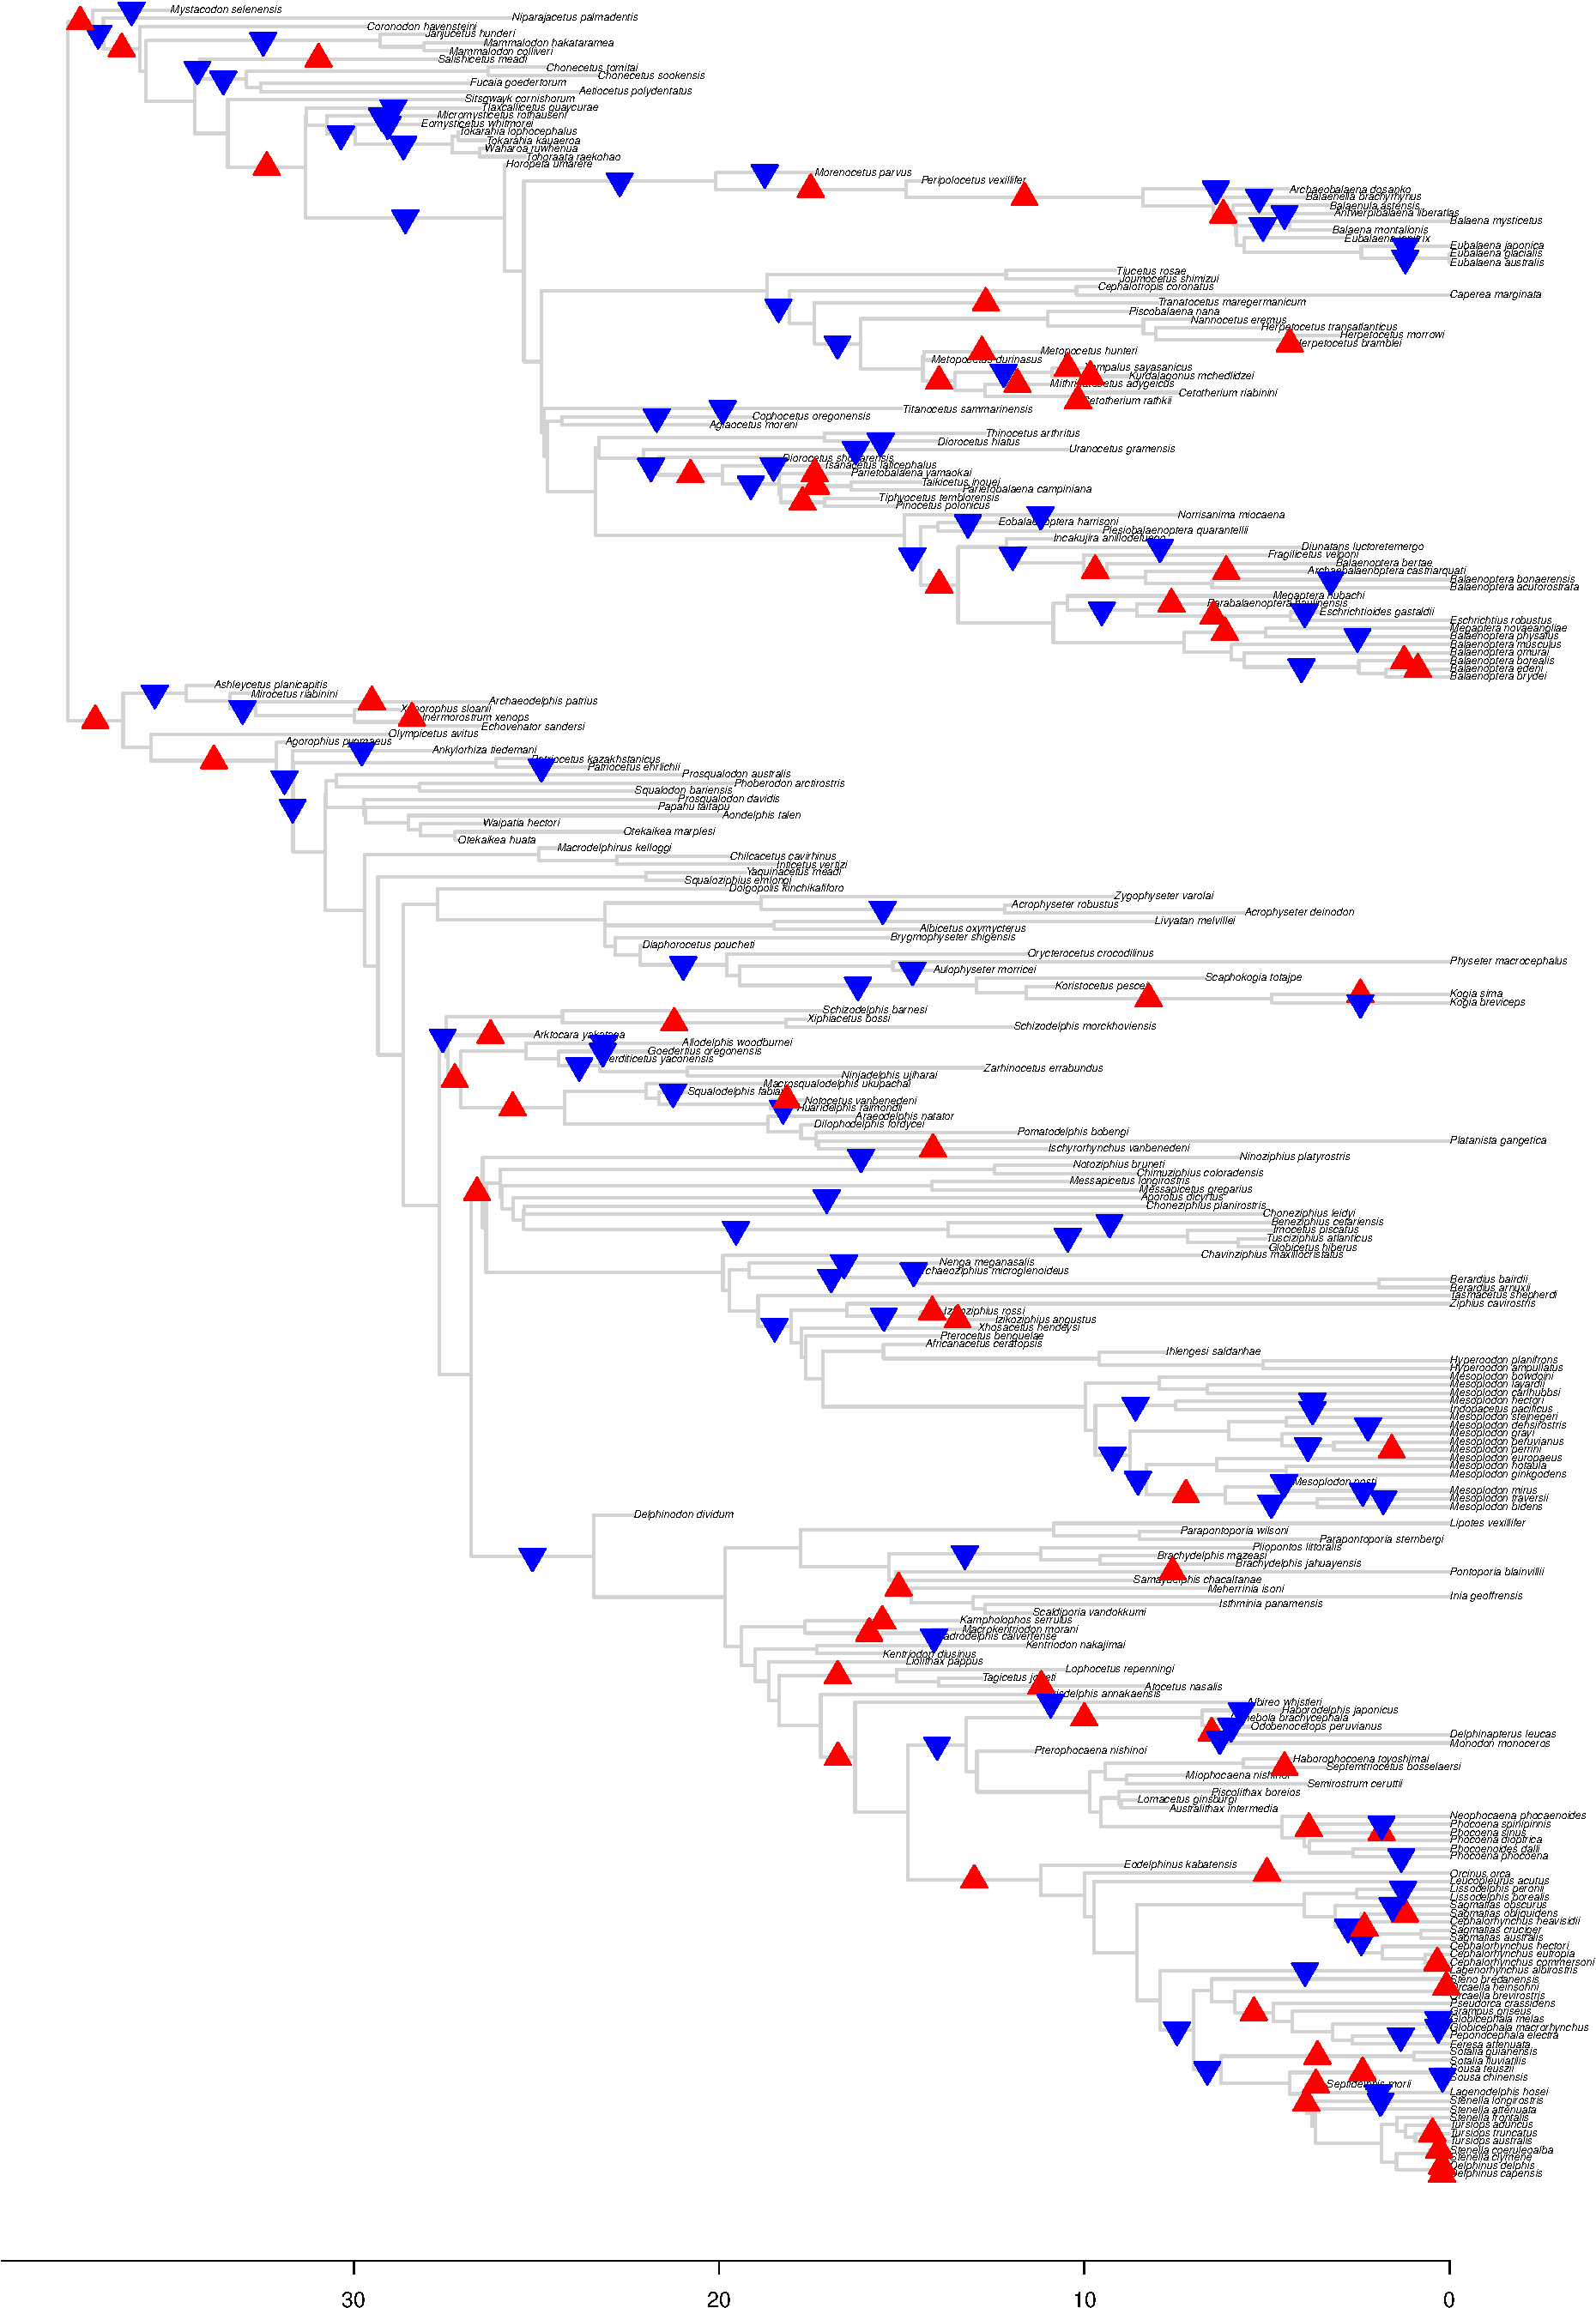
\includegraphics[width=0.9\textwidth]{img/plots-noarchaeo-k50-1.pdf}
\caption{Results for \textit{bayou} fit for the \textit{No Archaeoceti} tree, excluding taxa on zero-length branches, setting the average number of shifts in the prior distribution ($\lambda$) to 50. The triangles represent the position and direction of the shifts with posterior probability higher than 0.1, with upward triangles (in red) indicating increases in $\theta$, and downward triangles (in blue) indicating decreases in $\theta$.}
\label{fig:noarchaeo-k50-nzlb}
\end{figure}

%---------------------------------------------------------------------
\subsubsection{\textit{No Extant} tree}
%---------------------------------------------------------------------

\begin{figure}[H]
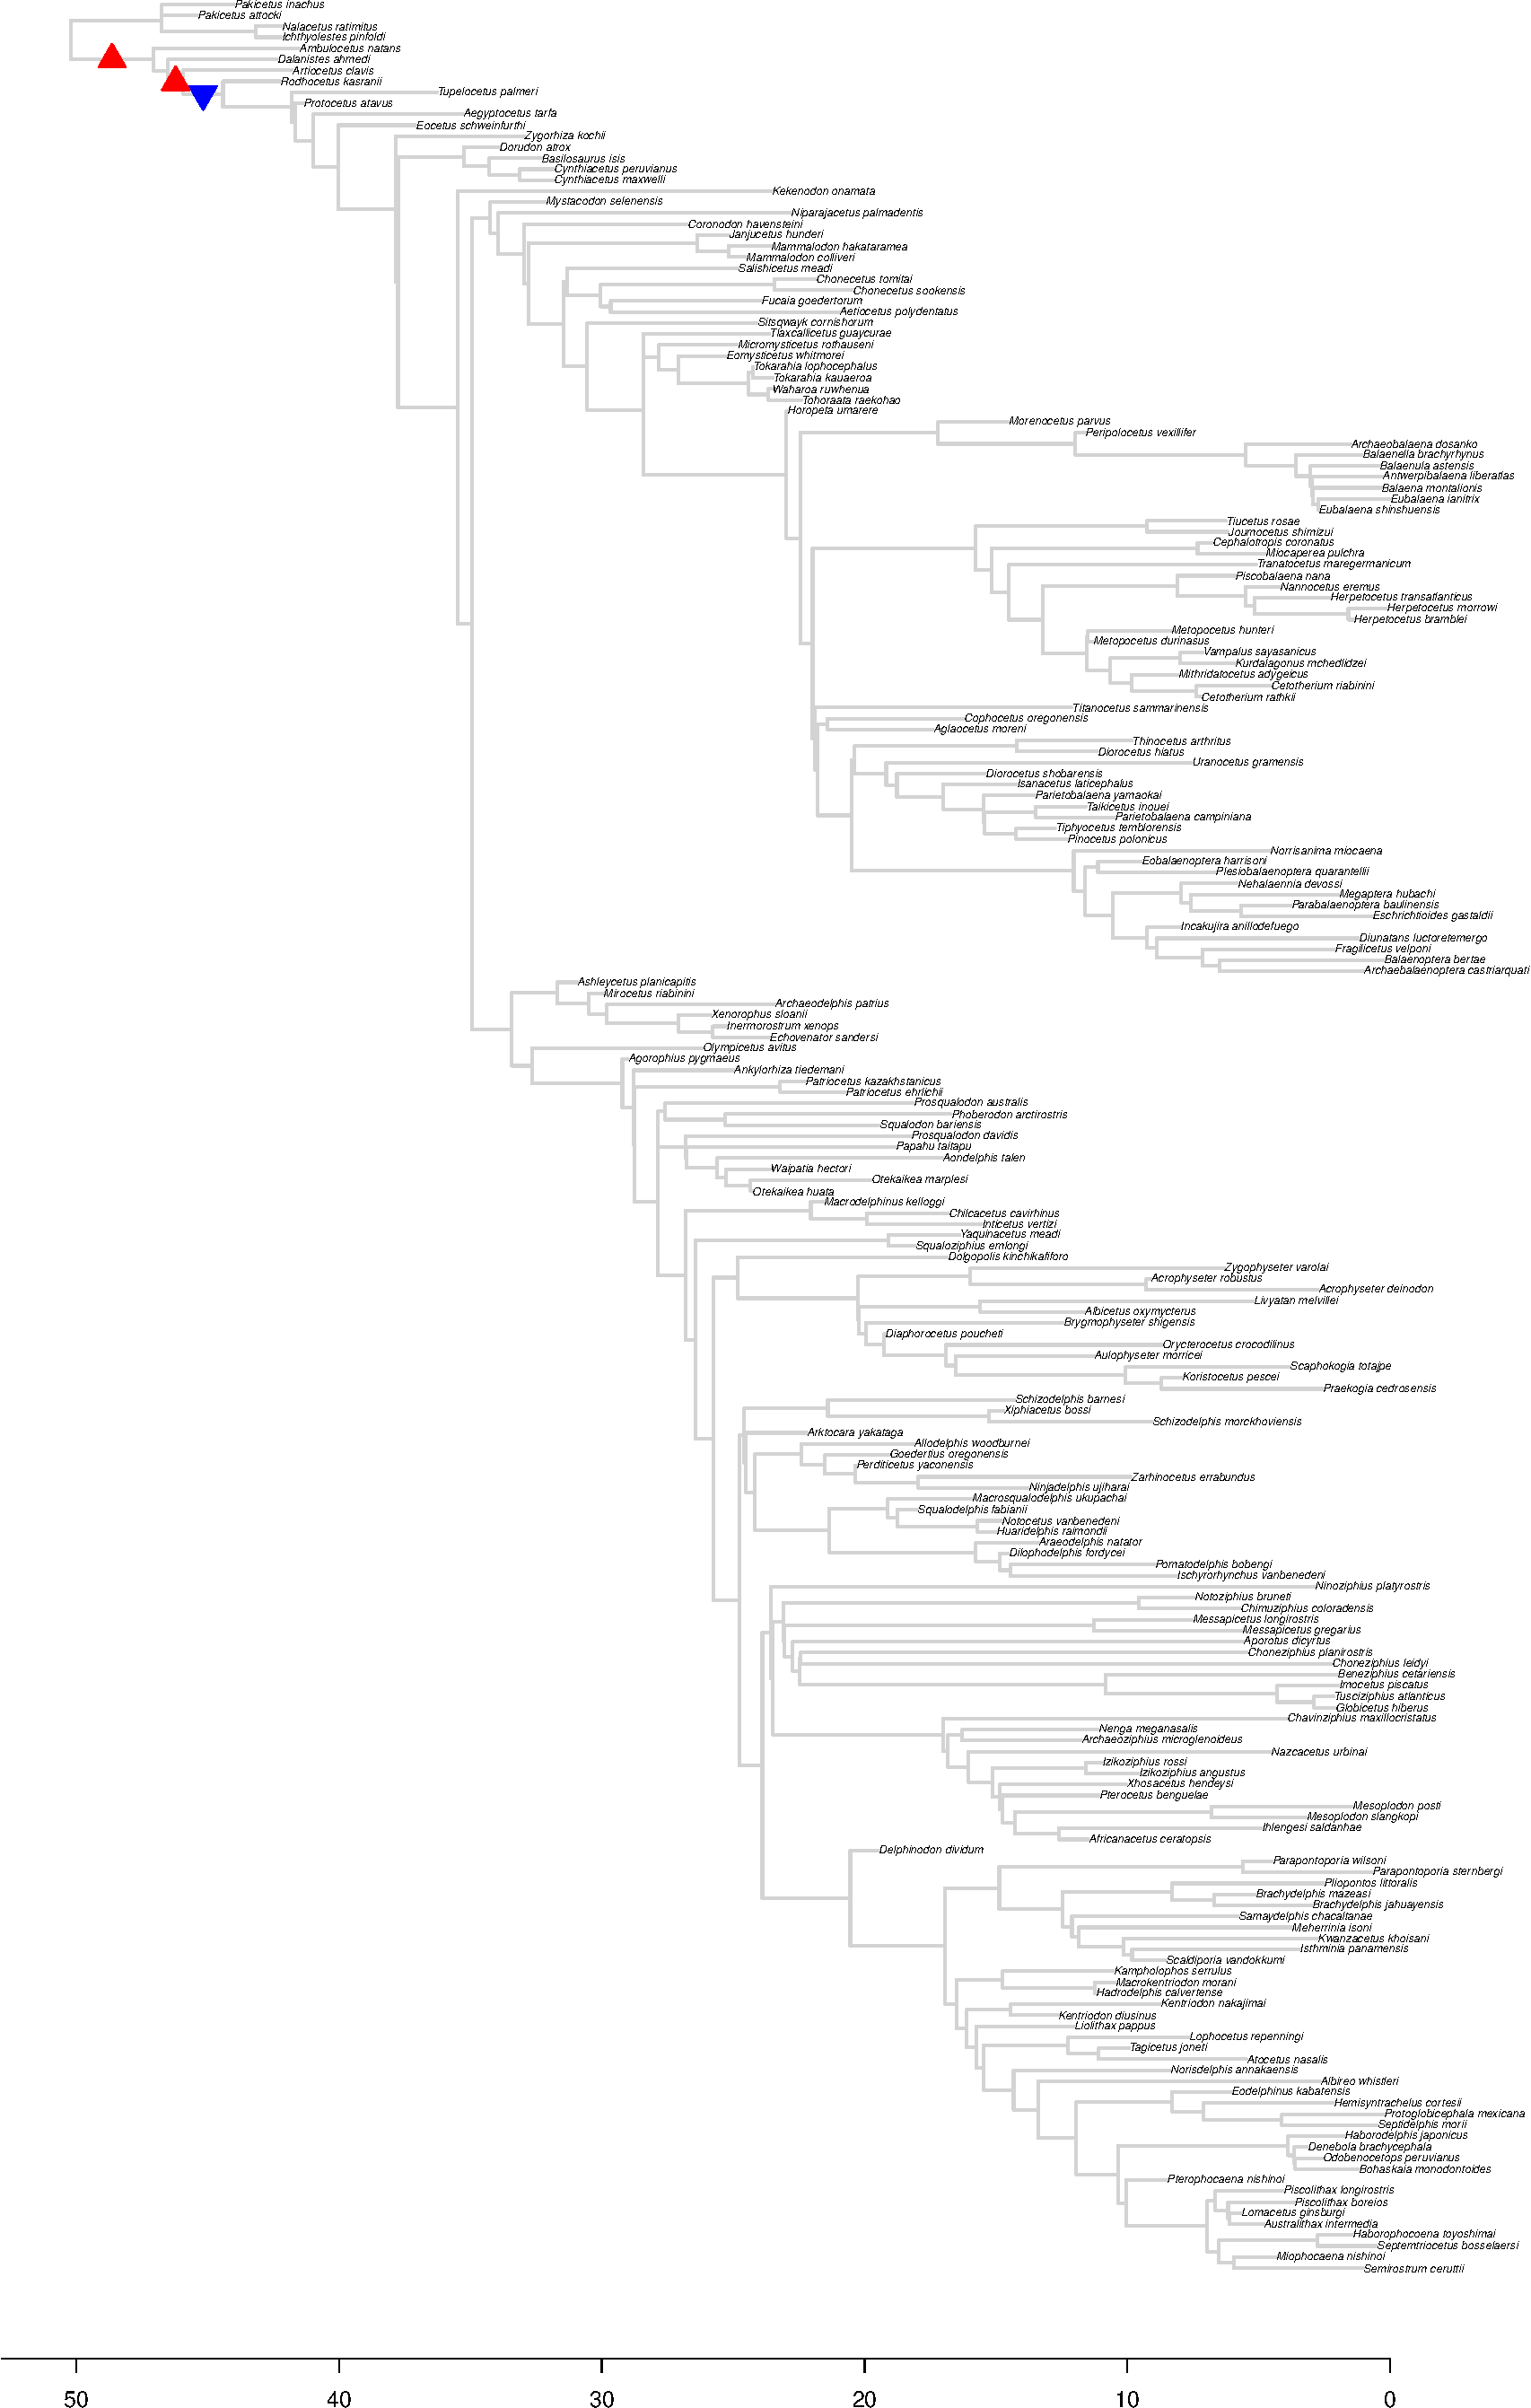
\includegraphics[width=0.8\textwidth]{img/plots-noextant-k5-1.pdf}
\caption{Results for \textit{bayou} fit for the \textit{No Extant} tree, excluding taxa on zero-length branches, setting the average number of shifts in the prior distribution ($\lambda$) to 5. The triangles represent the position and direction of the shifts with posterior probability higher than 0.1, with upward triangles (in red) indicating increases in $\theta$, and downward triangles (in blue) indicating decreases in $\theta$.}
\label{fig:extant-k5-nzlb}
\end{figure}

\newpage

\begin{figure}[H]
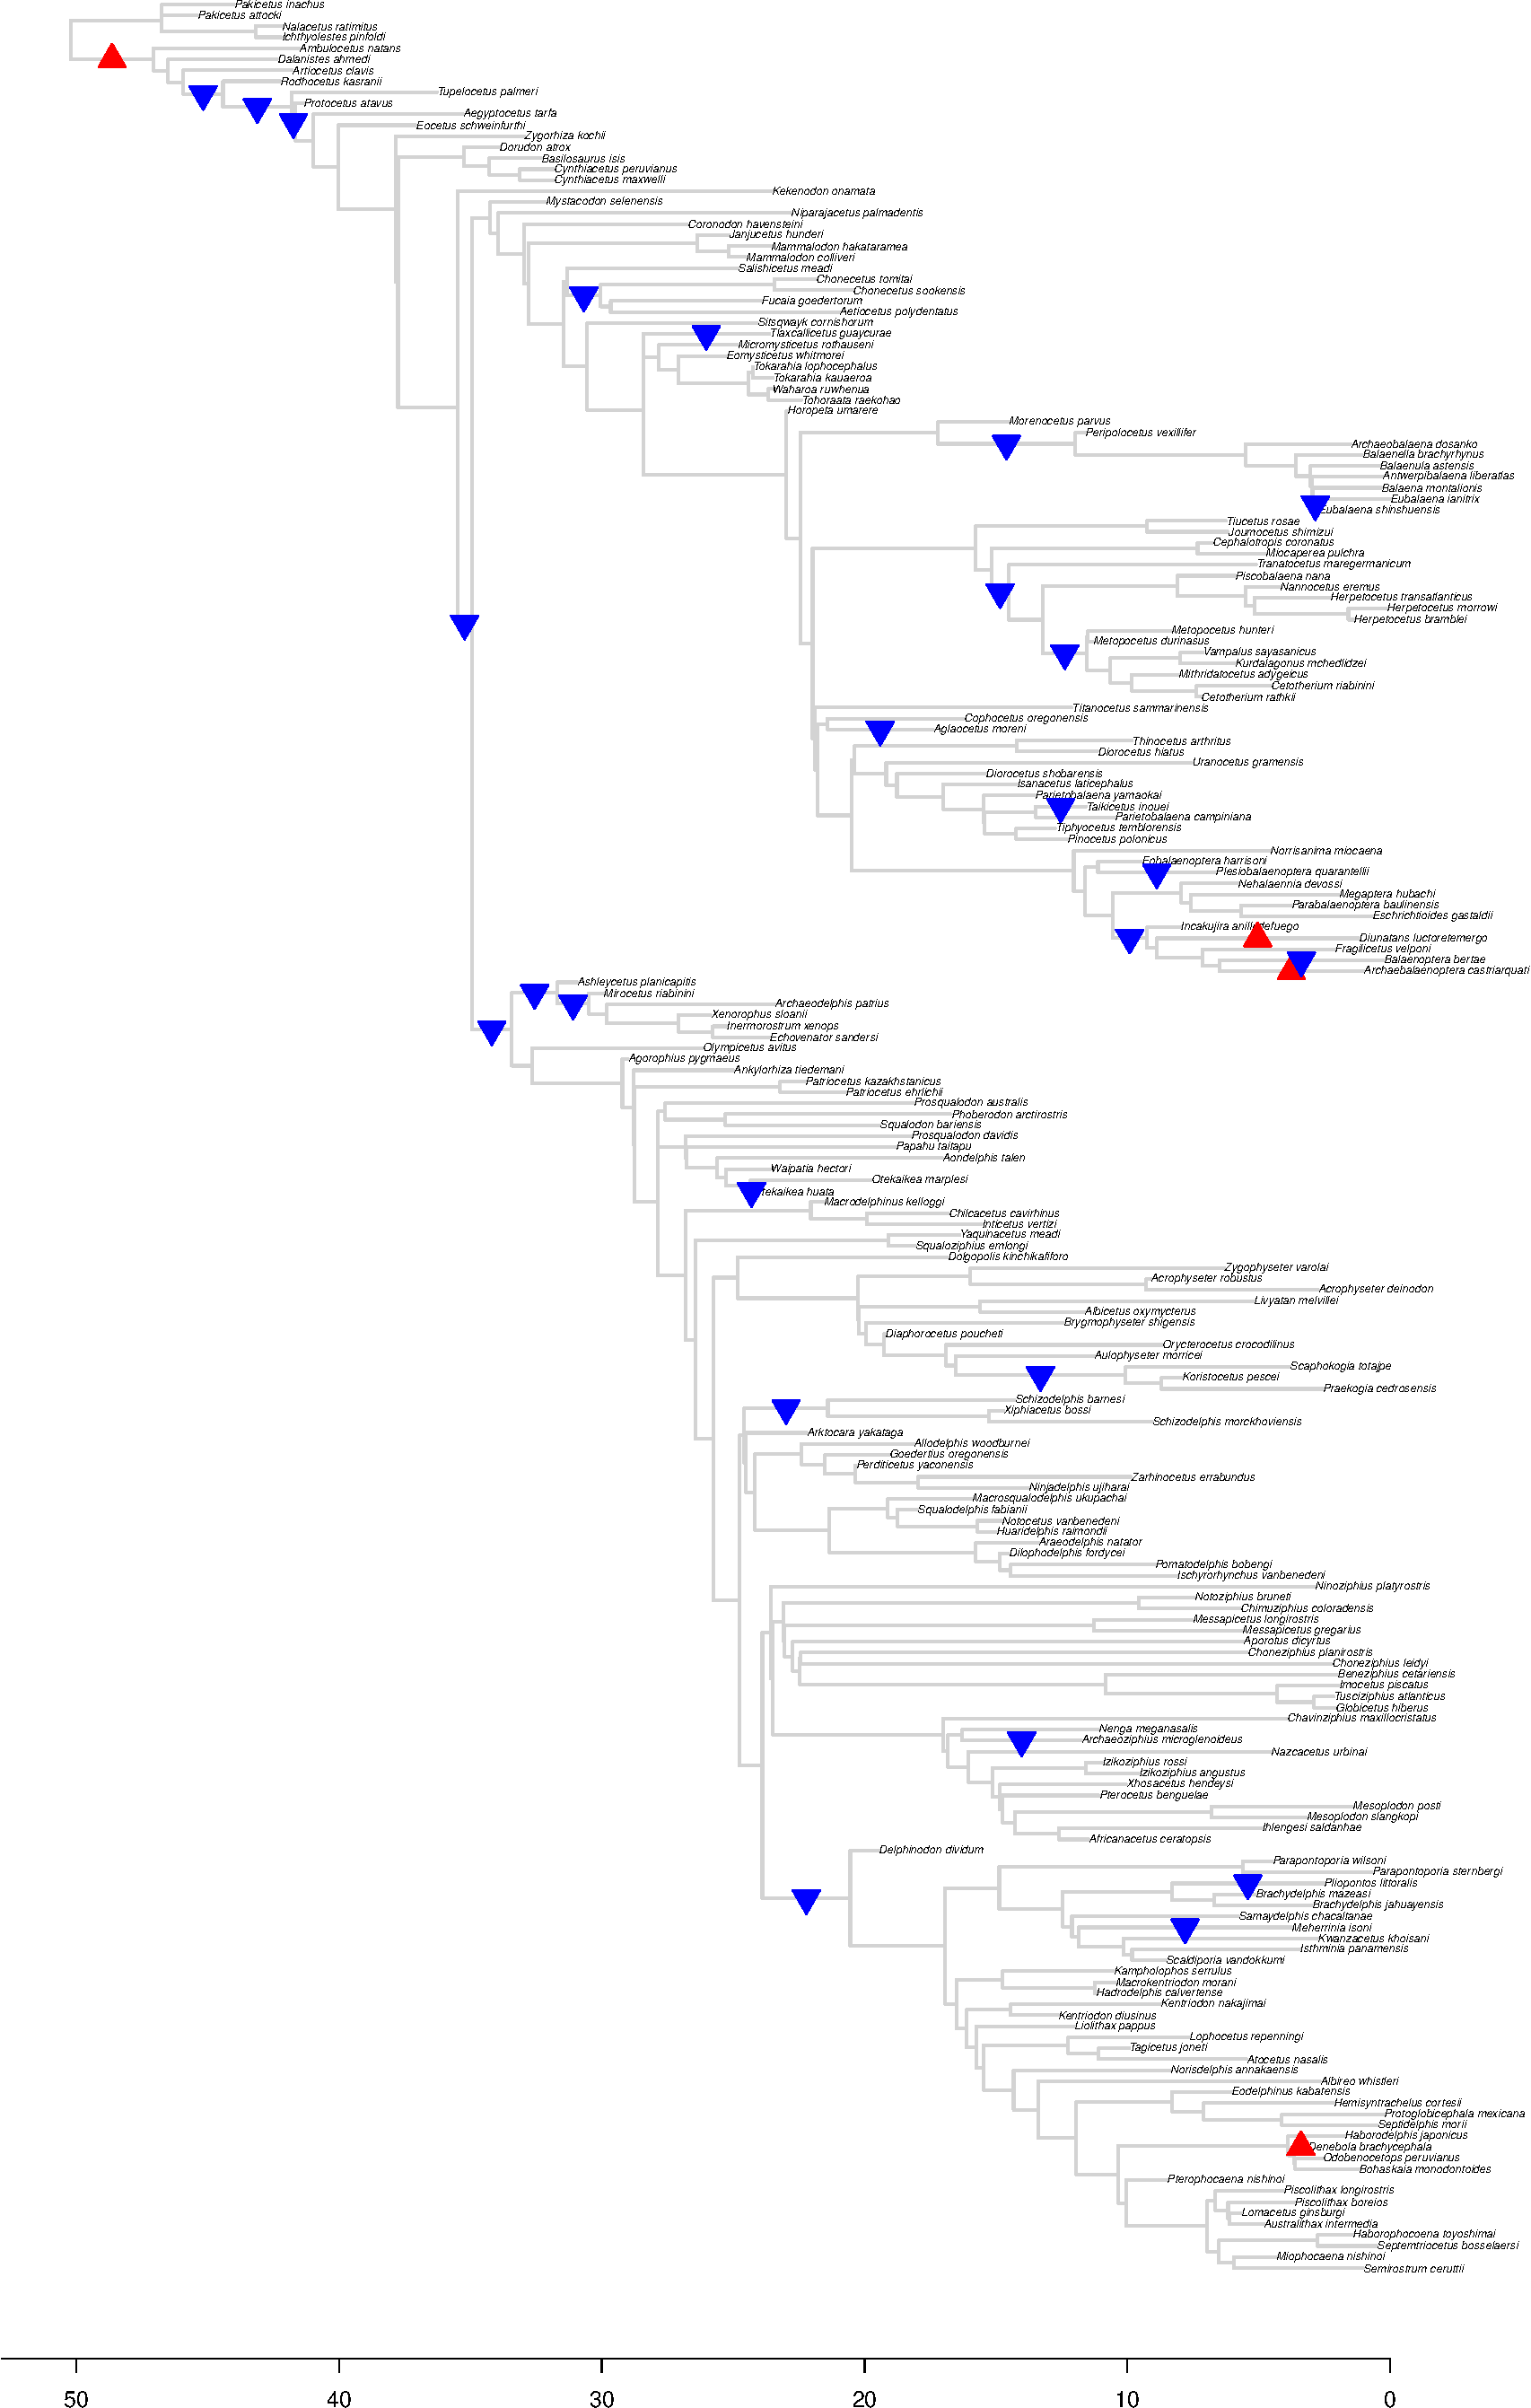
\includegraphics[width=0.9\textwidth]{img/plots-noextant-k15-1.pdf}
\caption{Results for \textit{bayou} fit for the \textit{No Extant} tree, excluding taxa on zero-length branches, setting the average number of shifts in the prior distribution ($\lambda$) to 15. The triangles represent the position and direction of the shifts with posterior probability higher than 0.1, with upward triangles (in red) indicating increases in $\theta$, and downward triangles (in blue) indicating decreases in $\theta$.}
\label{fig:extant-k15-nzlb}
\end{figure}

\newpage

\begin{figure}[H]
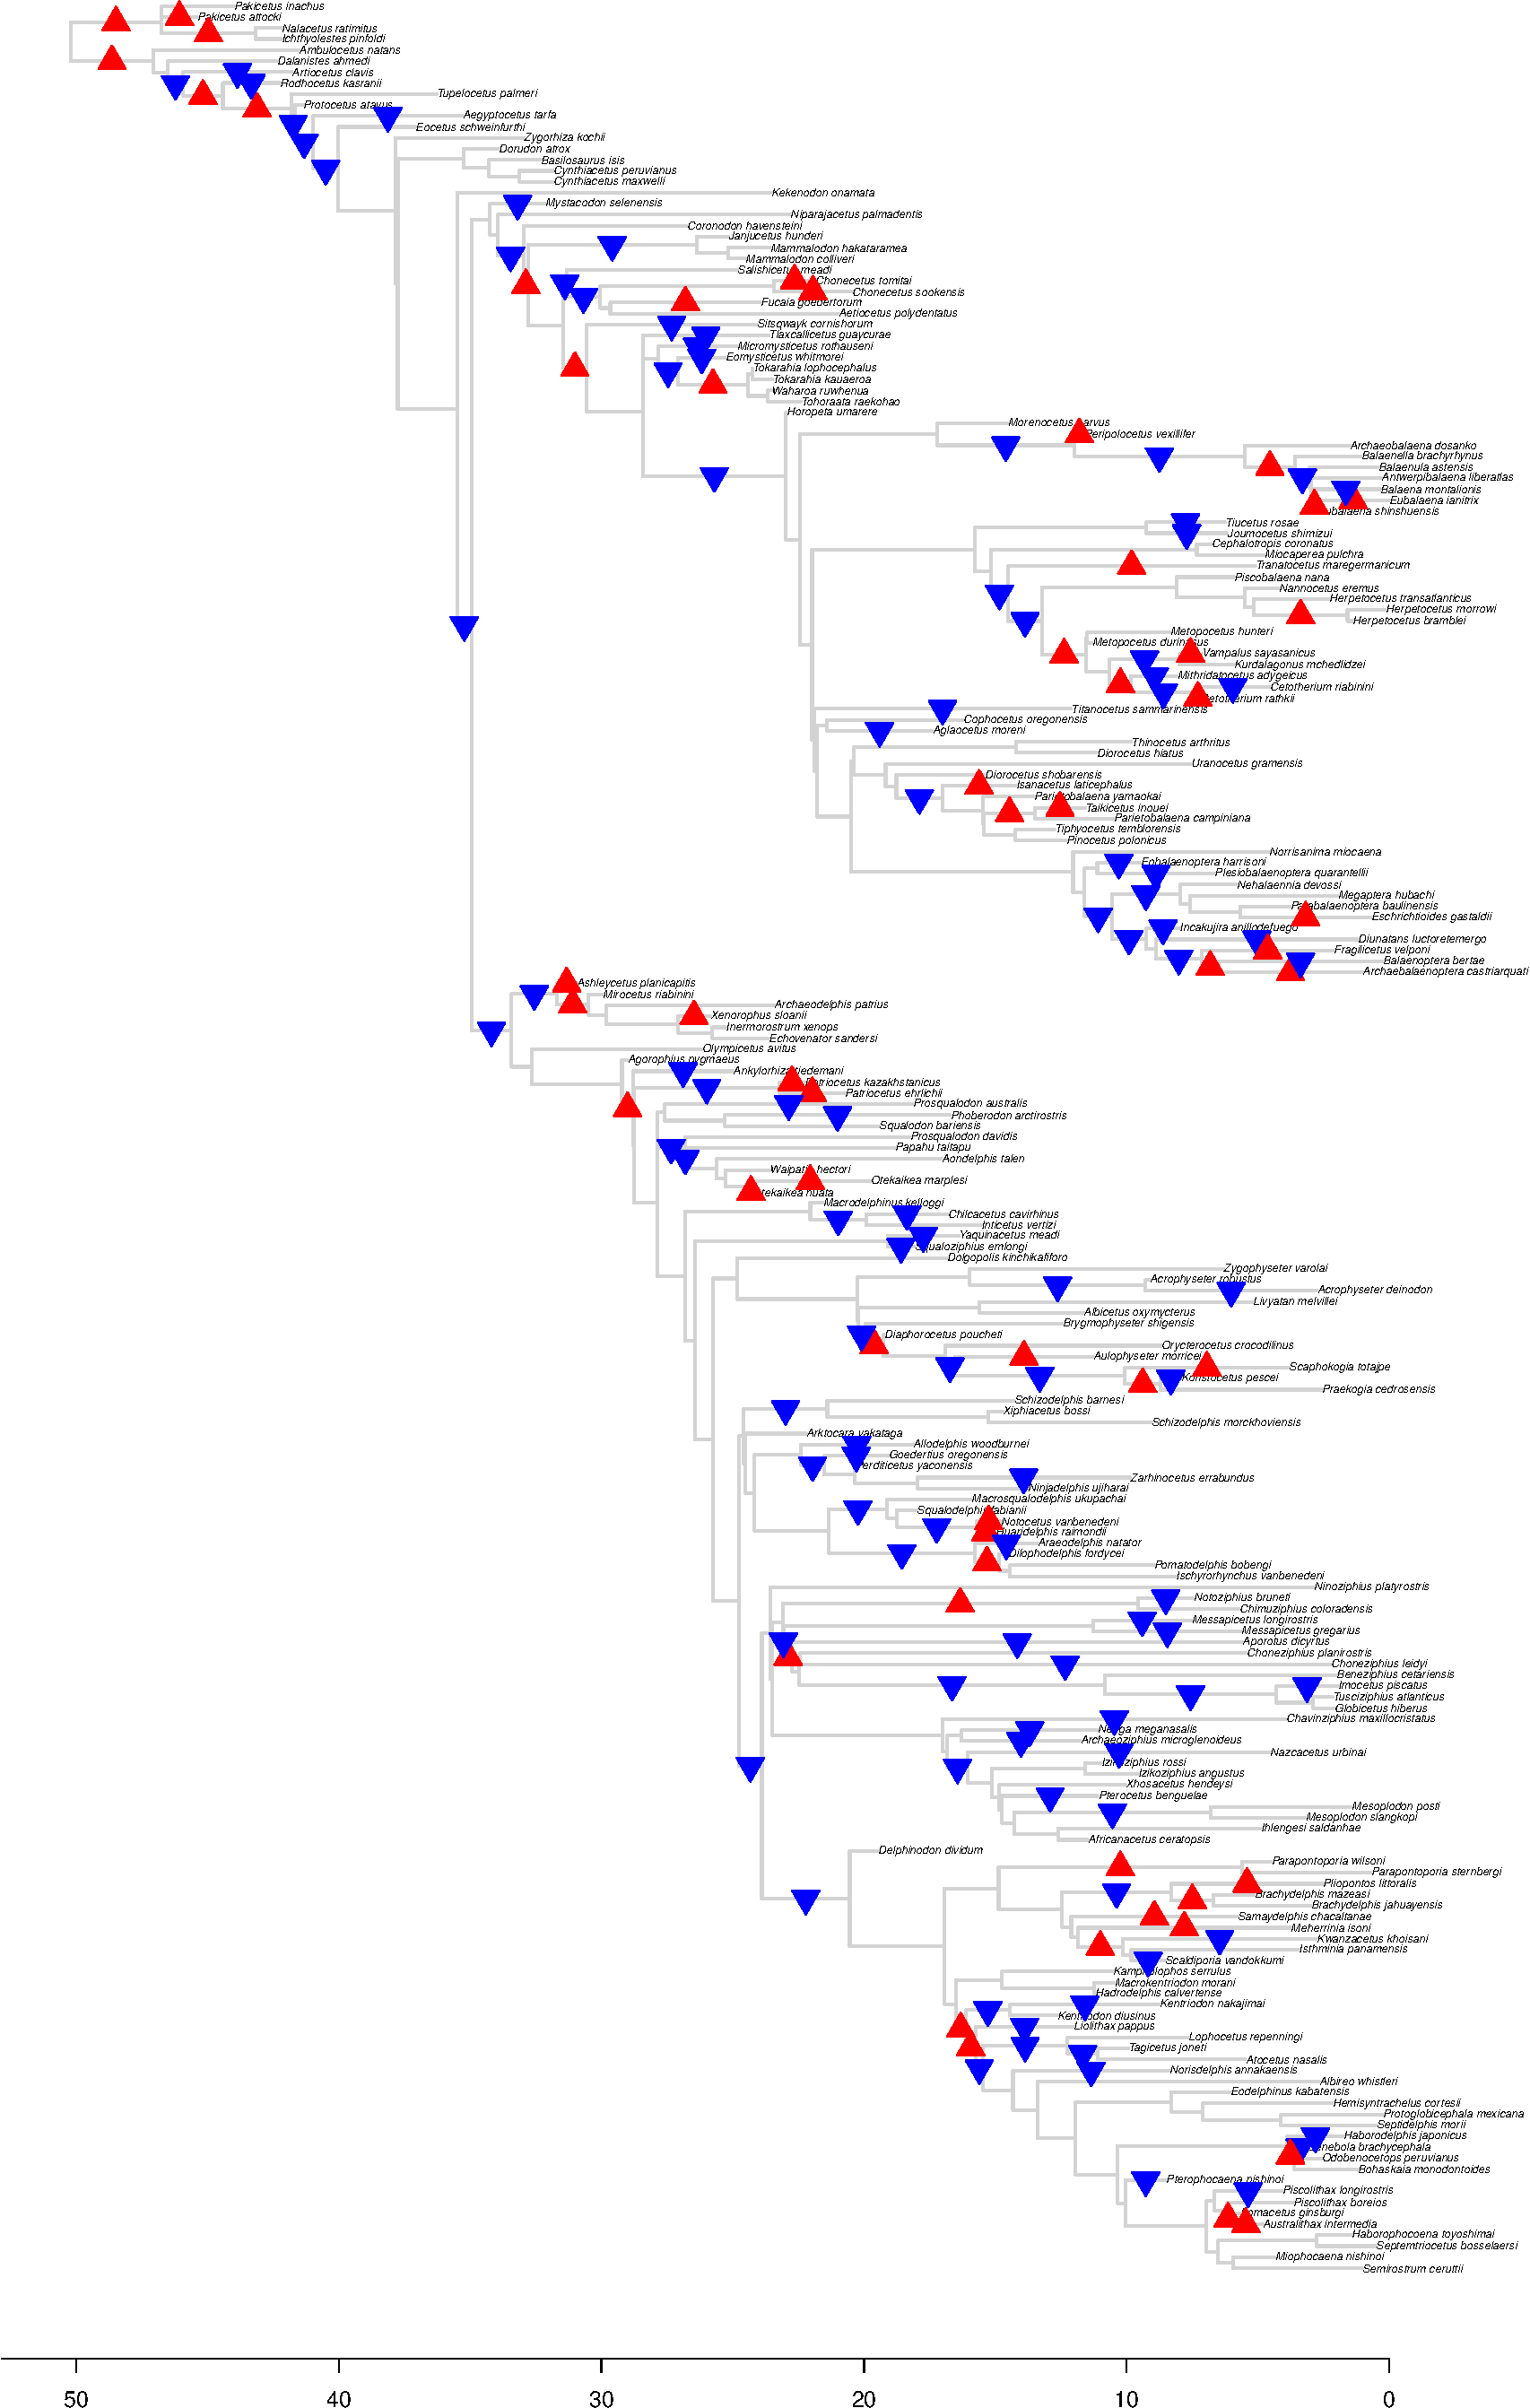
\includegraphics[width=0.9\textwidth]{img/plots-noextant-k50-1.pdf}
\caption{Results for \textit{bayou} fit for the \textit{No Extant} tree, excluding taxa on zero-length branches, setting the average number of shifts in the prior distribution ($\lambda$) to 50. The triangles represent the position and direction of the shifts with posterior probability higher than 0.1, with upward triangles (in red) indicating increases in $\theta$, and downward triangles (in blue) indicating decreases in $\theta$.}
\label{fig:extant-k50-nzlb}
\end{figure}

\newpage

\begin{figure}[H]
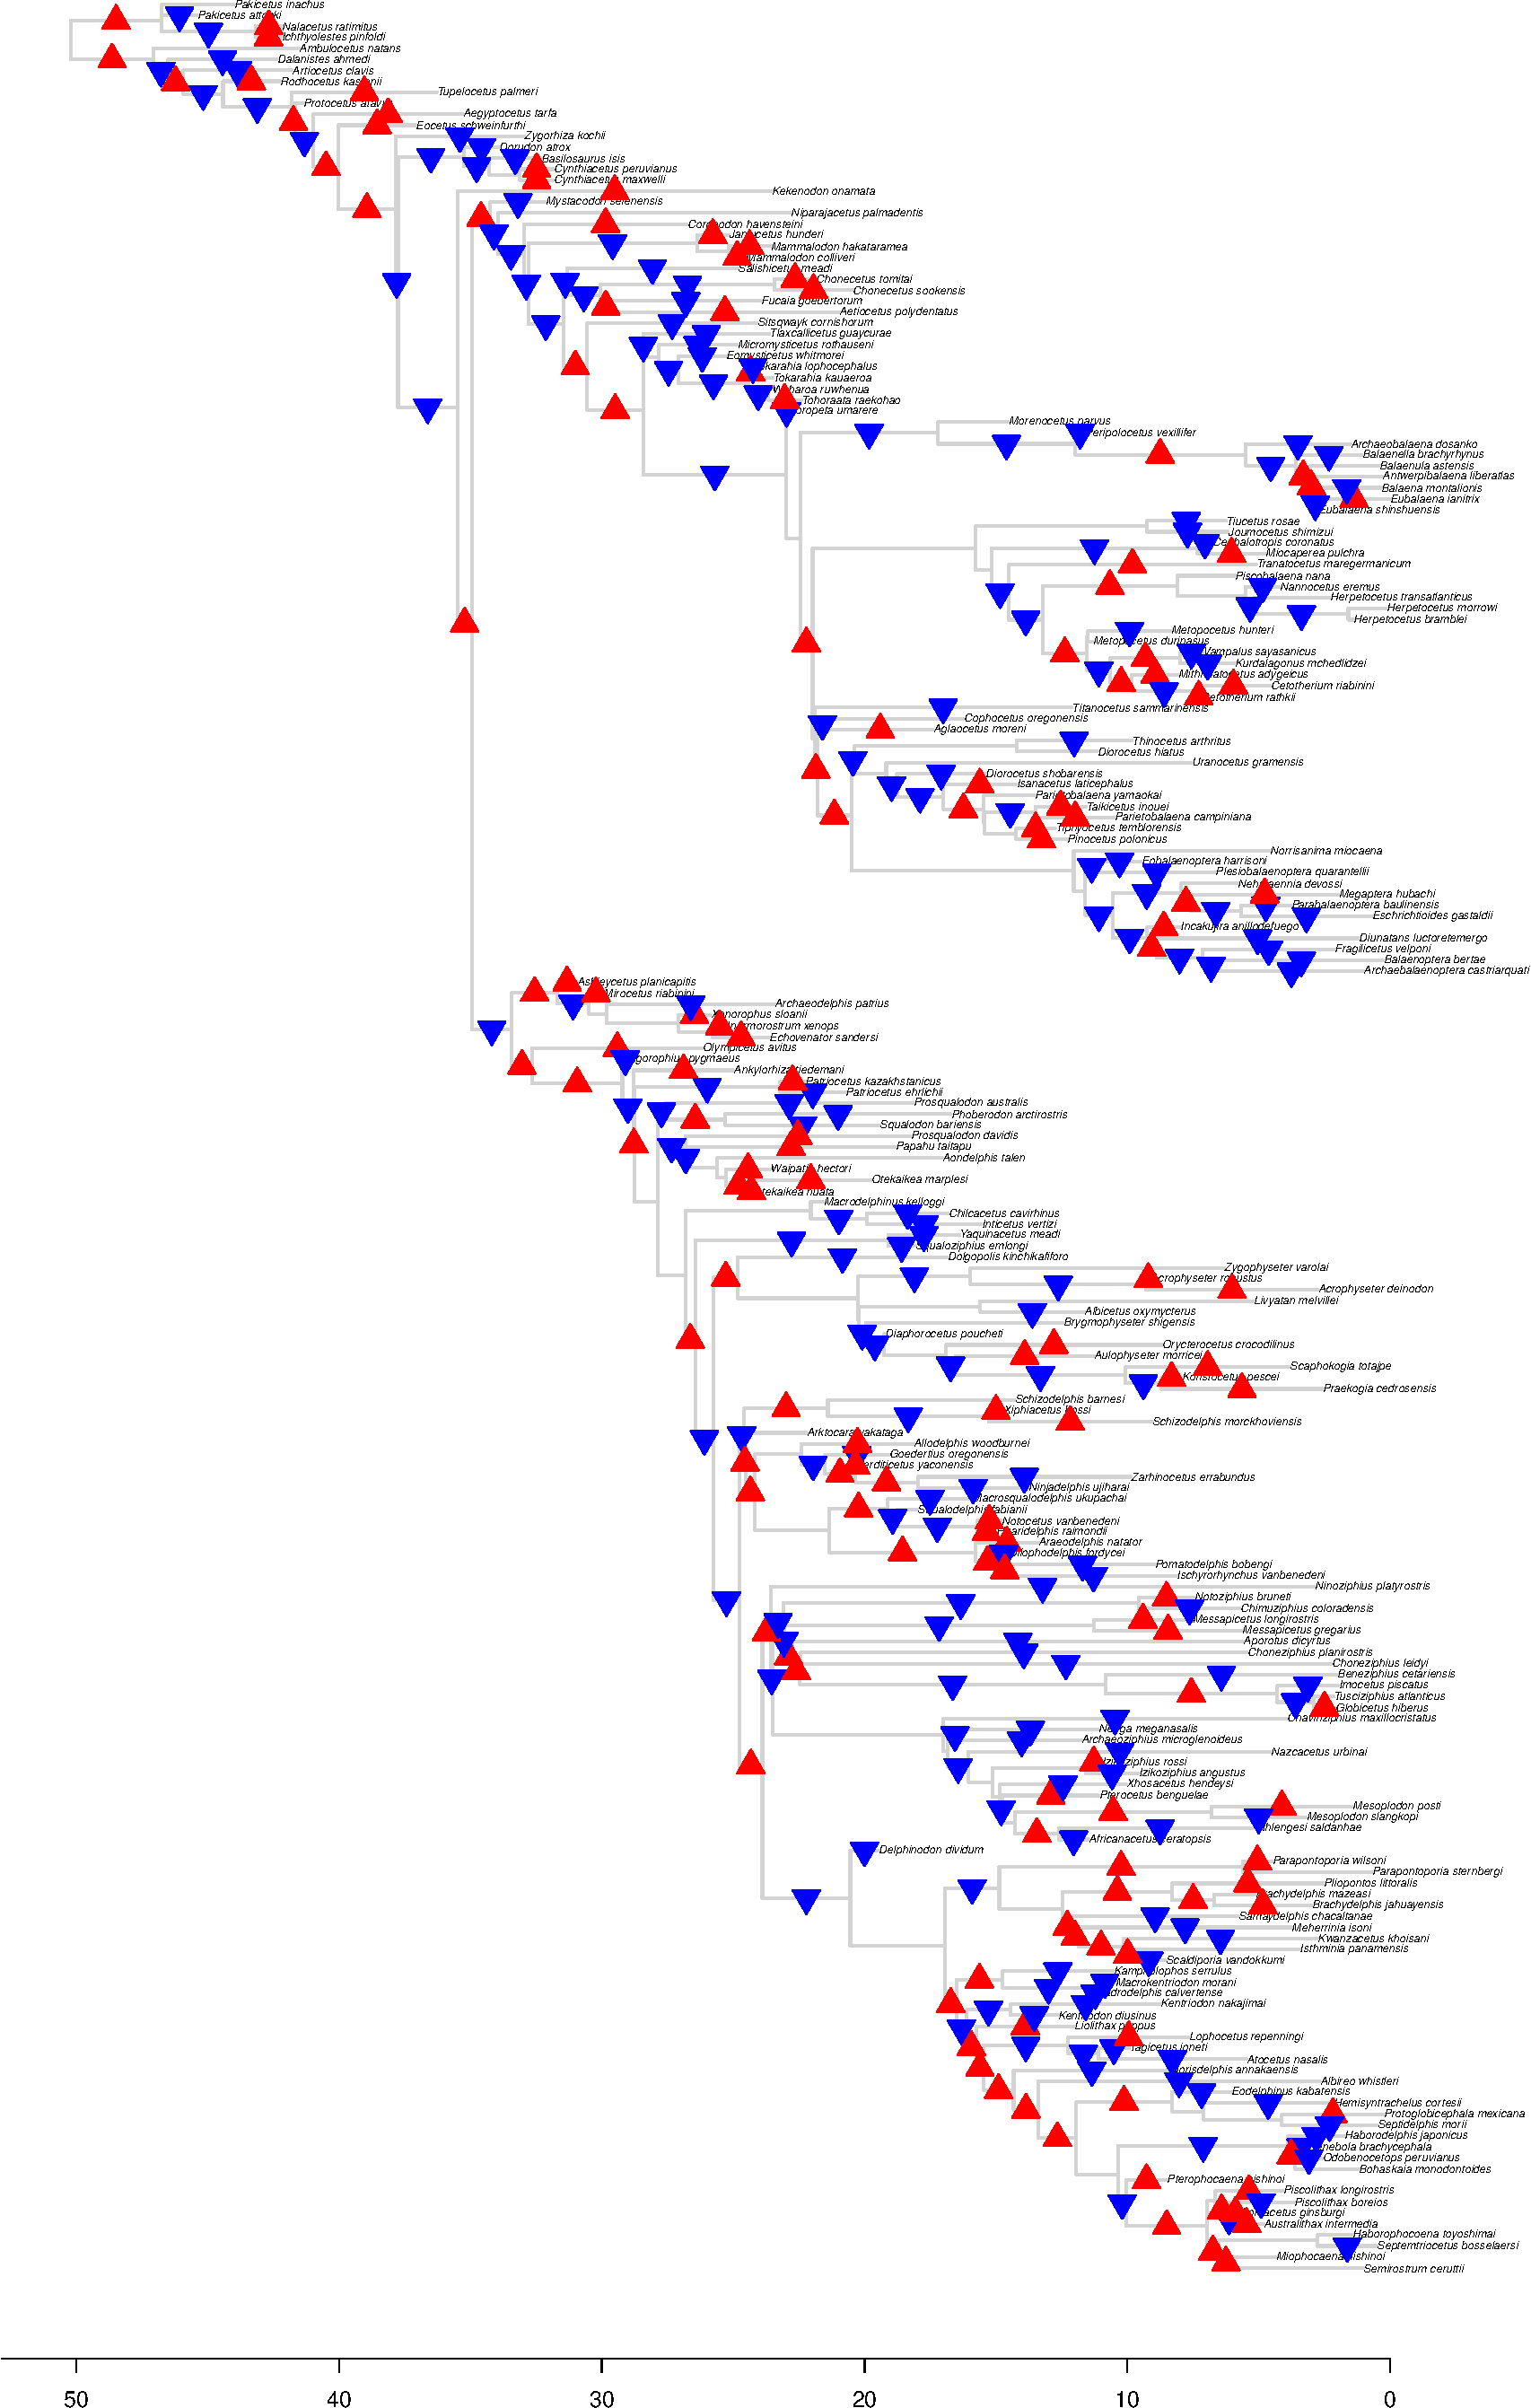
\includegraphics[width=0.9\textwidth]{img/plots-noextant-k250-1.pdf}
\caption{Results for \textit{bayou} fit for the \textit{No Extant} tree, excluding taxa on zero-length branches, setting the average number of shifts in the prior distribution ($\lambda$) to 250. The triangles represent the position and direction of the shifts with posterior probability higher than 0.1, with upward triangles (in red) indicating increases in $\theta$, and downward triangles (in blue) indicating decreases in $\theta$.}
\label{fig:extant-k250-nzlb}
\end{figure}

\newpage

\begin{figure}[H]
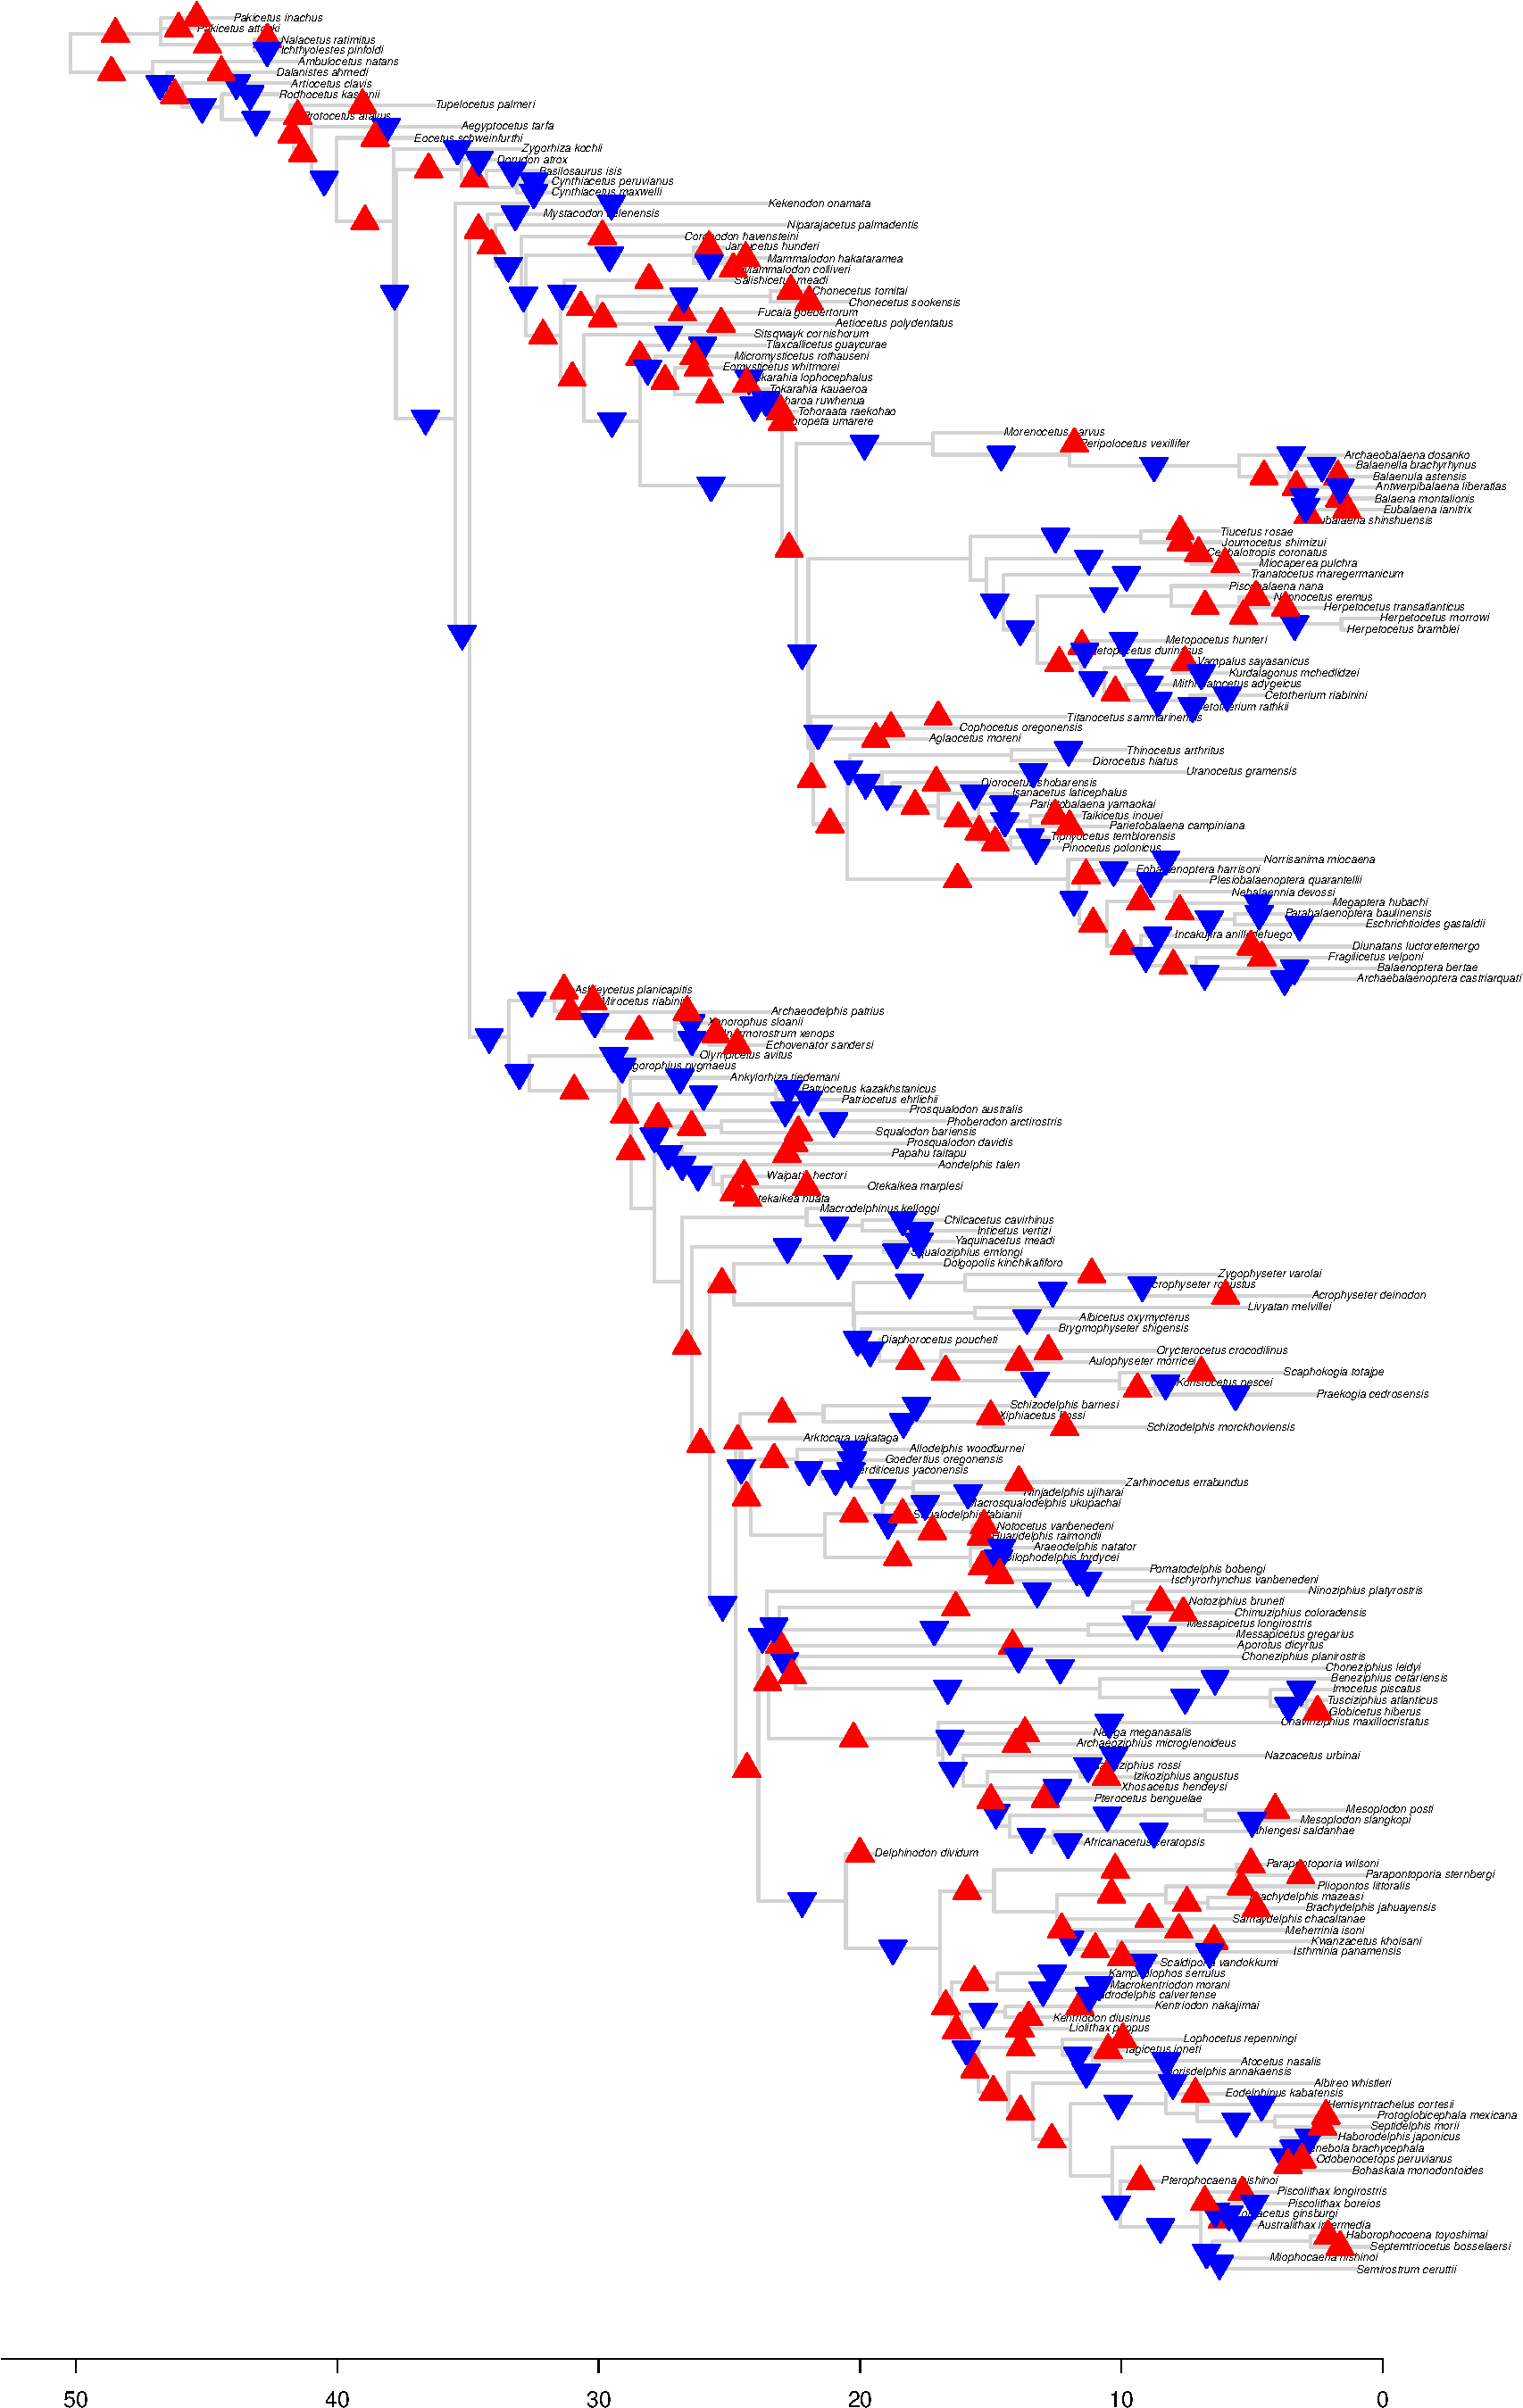
\includegraphics[width=0.9\textwidth]{img/plots-noextant-k500-1.pdf}
\caption{Results for \textit{bayou} fit for the \textit{No Extant} tree, excluding taxa on zero-length branches, setting the average number of shifts in the prior distribution ($\lambda$) to 500. The triangles represent the position and direction of the shifts with posterior probability higher than 0.1, with upward triangles (in red) indicating increases in $\theta$, and downward triangles (in blue) indicating decreases in $\theta$.}
\label{fig:extant-k500-nzlb}
\end{figure}

\newpage

%---------------------------------------------------------------------
\subsubsection{\textit{No Imput} tree}
%---------------------------------------------------------------------

\begin{figure}[H]
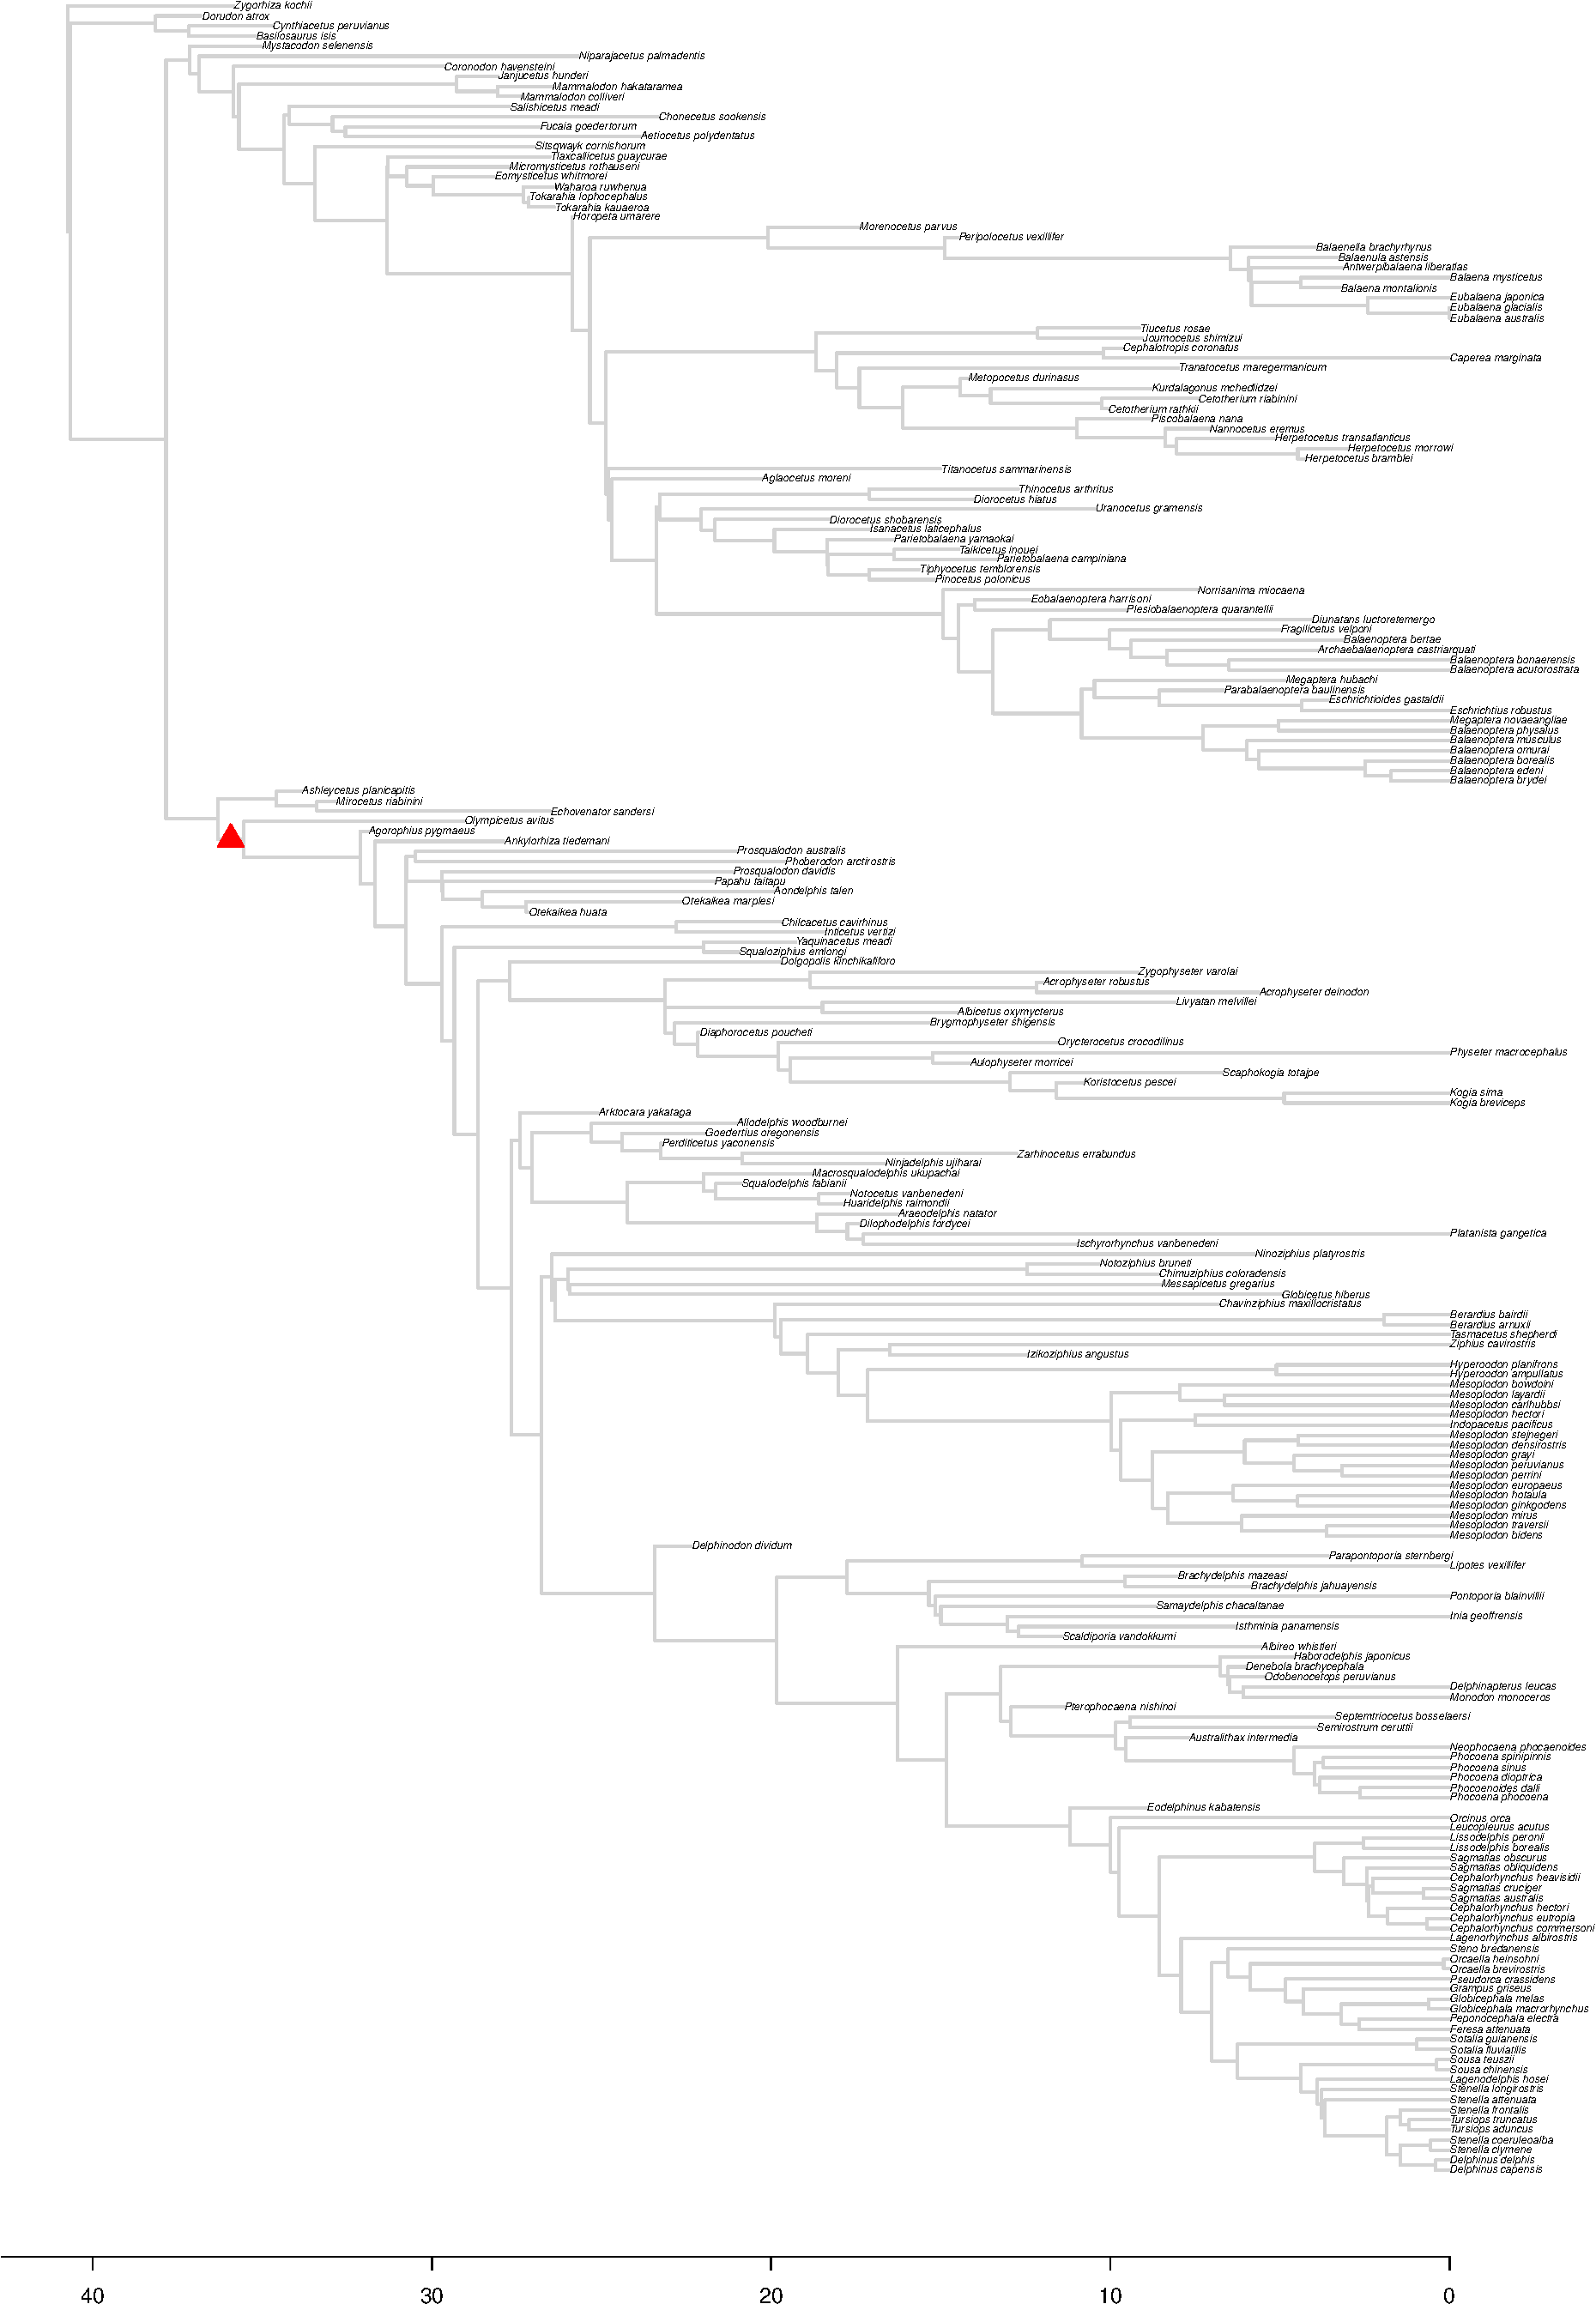
\includegraphics[width=0.8\textwidth]{img/plots-noimput-k5-1.pdf}
\caption{Results for \textit{bayou} fit for the \textit{No Imput} tree, excluding taxa on zero-length branches, setting the average number of shifts in the prior distribution ($\lambda$) to 5. The triangles represent the position and direction of the shifts with posterior probability higher than 0.1, with upward triangles (in red) indicating increases in $\theta$, and downward triangles (in blue) indicating decreases in $\theta$.}
\label{fig:noimput-k5-nzlb}
\end{figure}

\newpage

\begin{figure}[H]
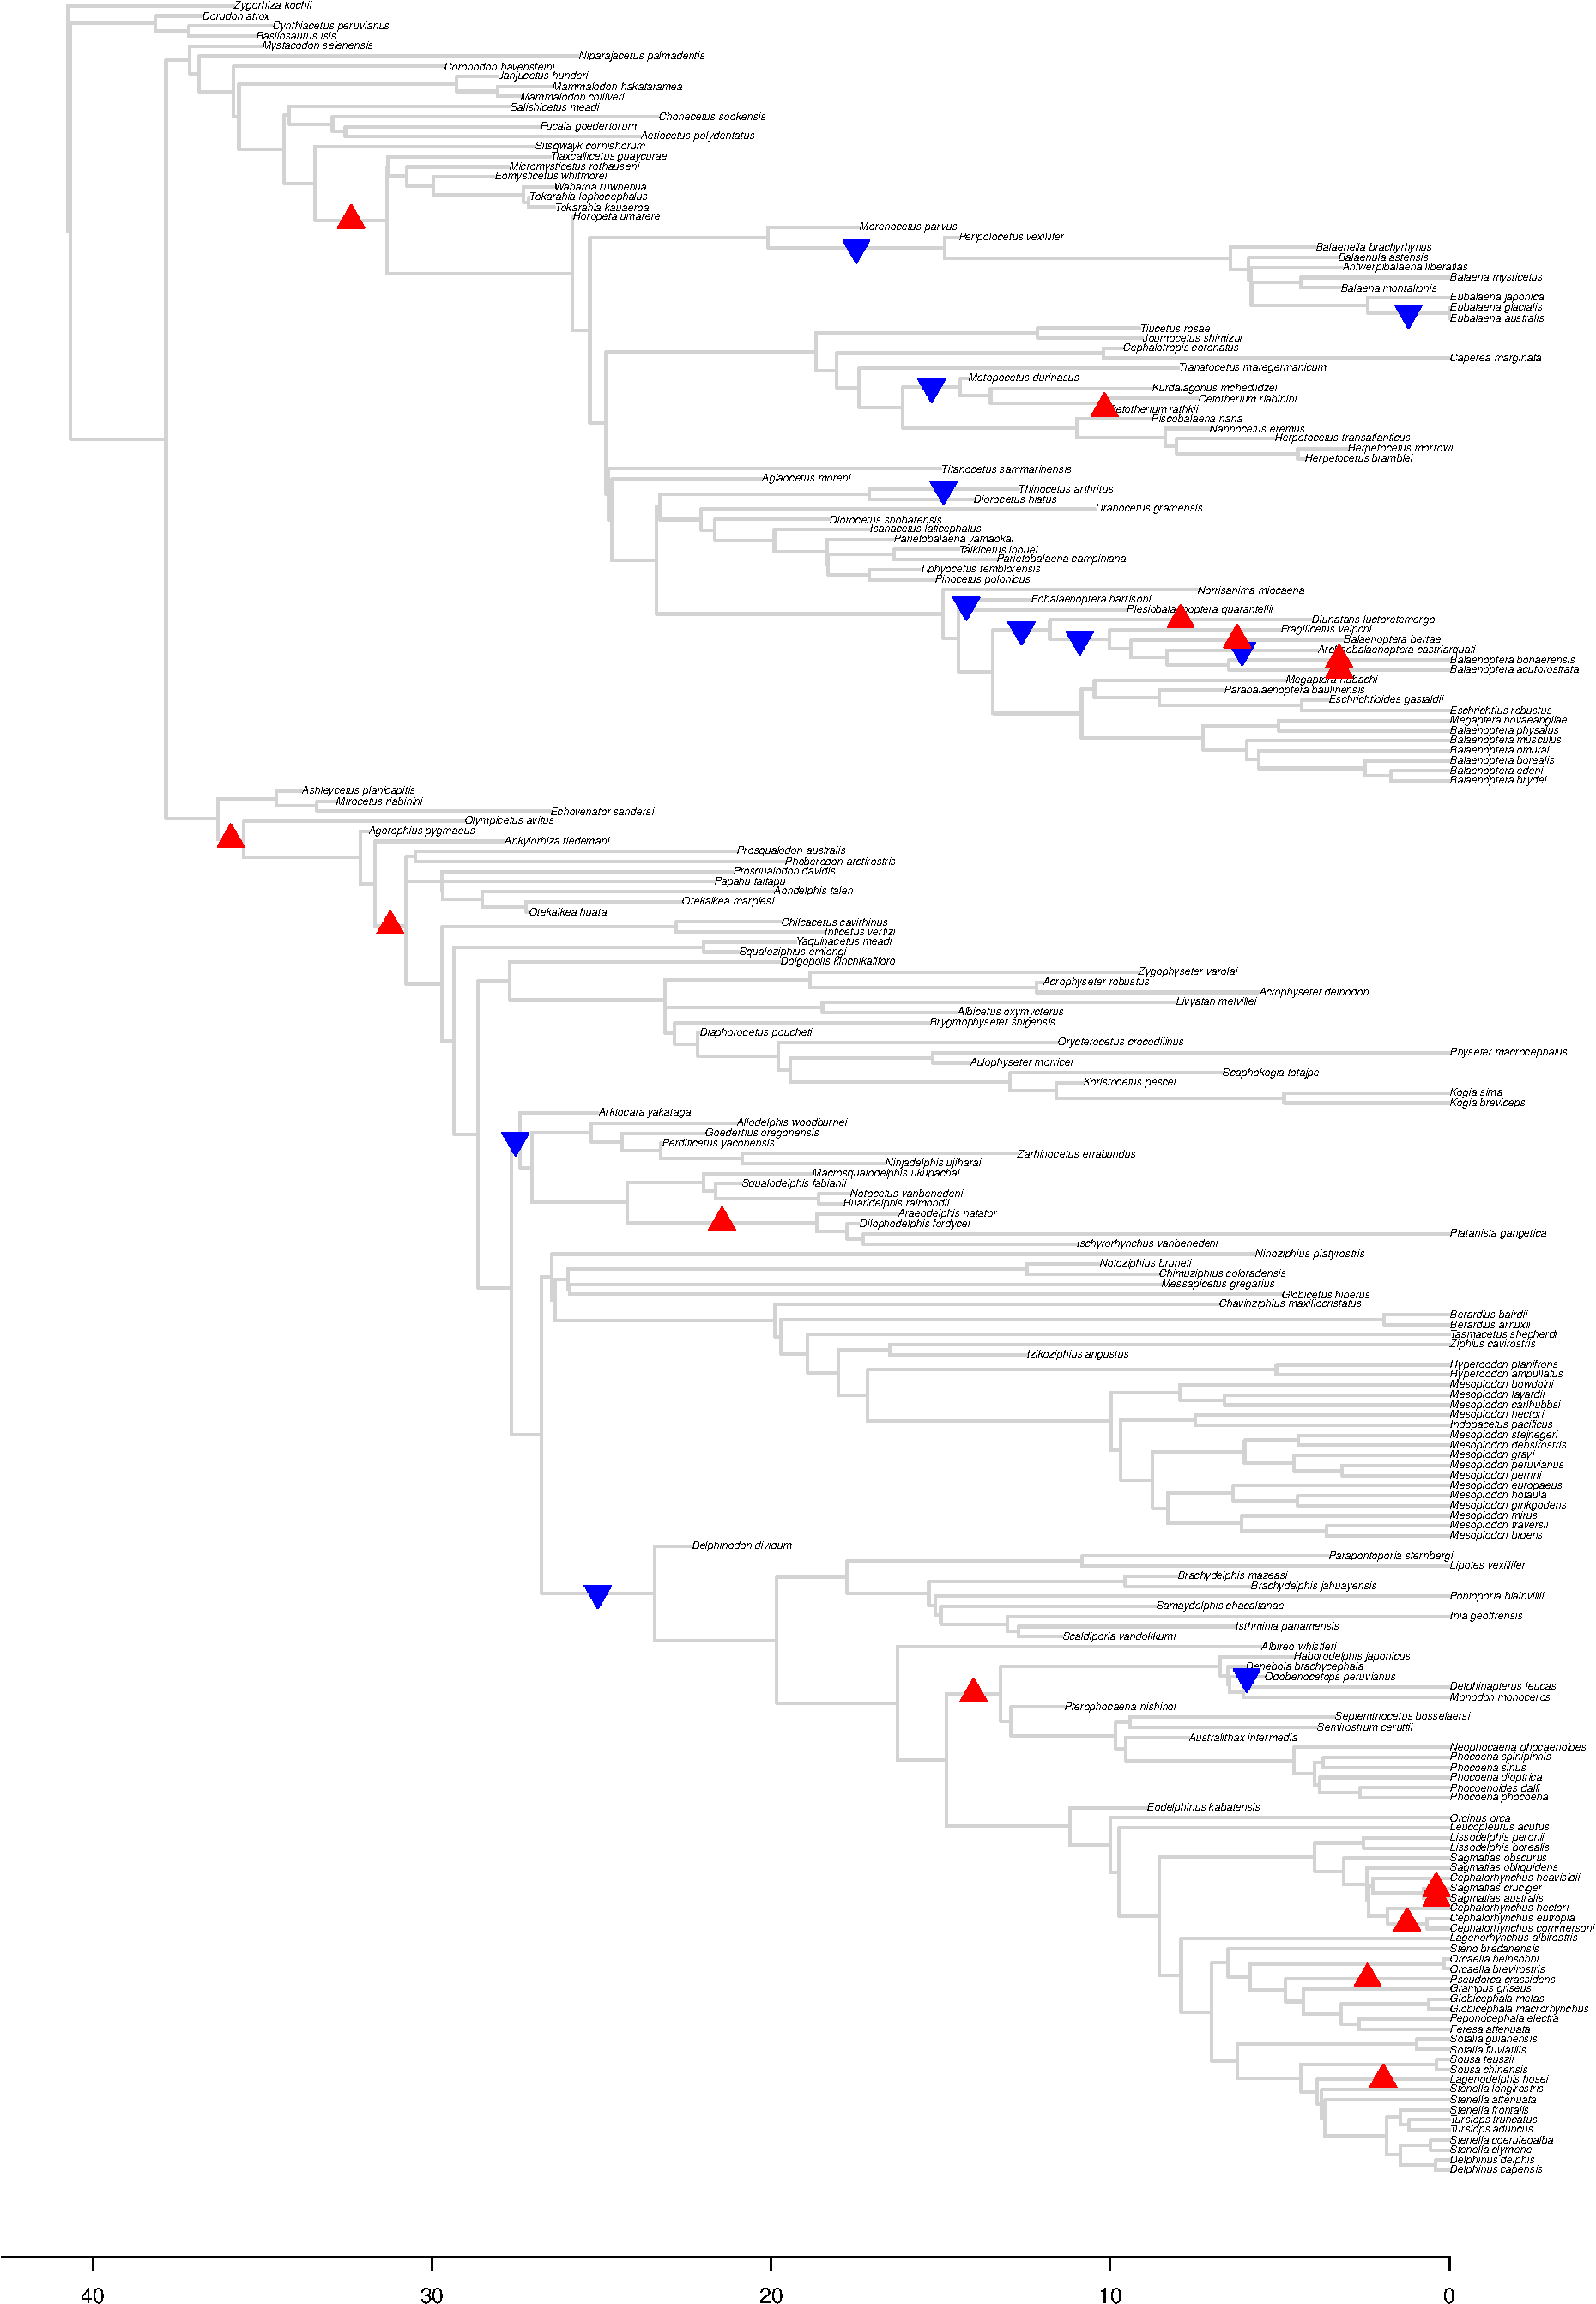
\includegraphics[width=0.9\textwidth]{img/plots-noimput-k15-1.pdf}
\caption{Results for \textit{bayou} fit for the \textit{No Imput} tree, excluding taxa on zero-length branches, setting the average number of shifts in the prior distribution ($\lambda$) to 15. The triangles represent the position and direction of the shifts with posterior probability higher than 0.1, with upward triangles (in red) indicating increases in $\theta$, and downward triangles (in blue) indicating decreases in $\theta$.}
\label{fig:noimput-k15-nzlb}
\end{figure}

\newpage

\begin{figure}[H]
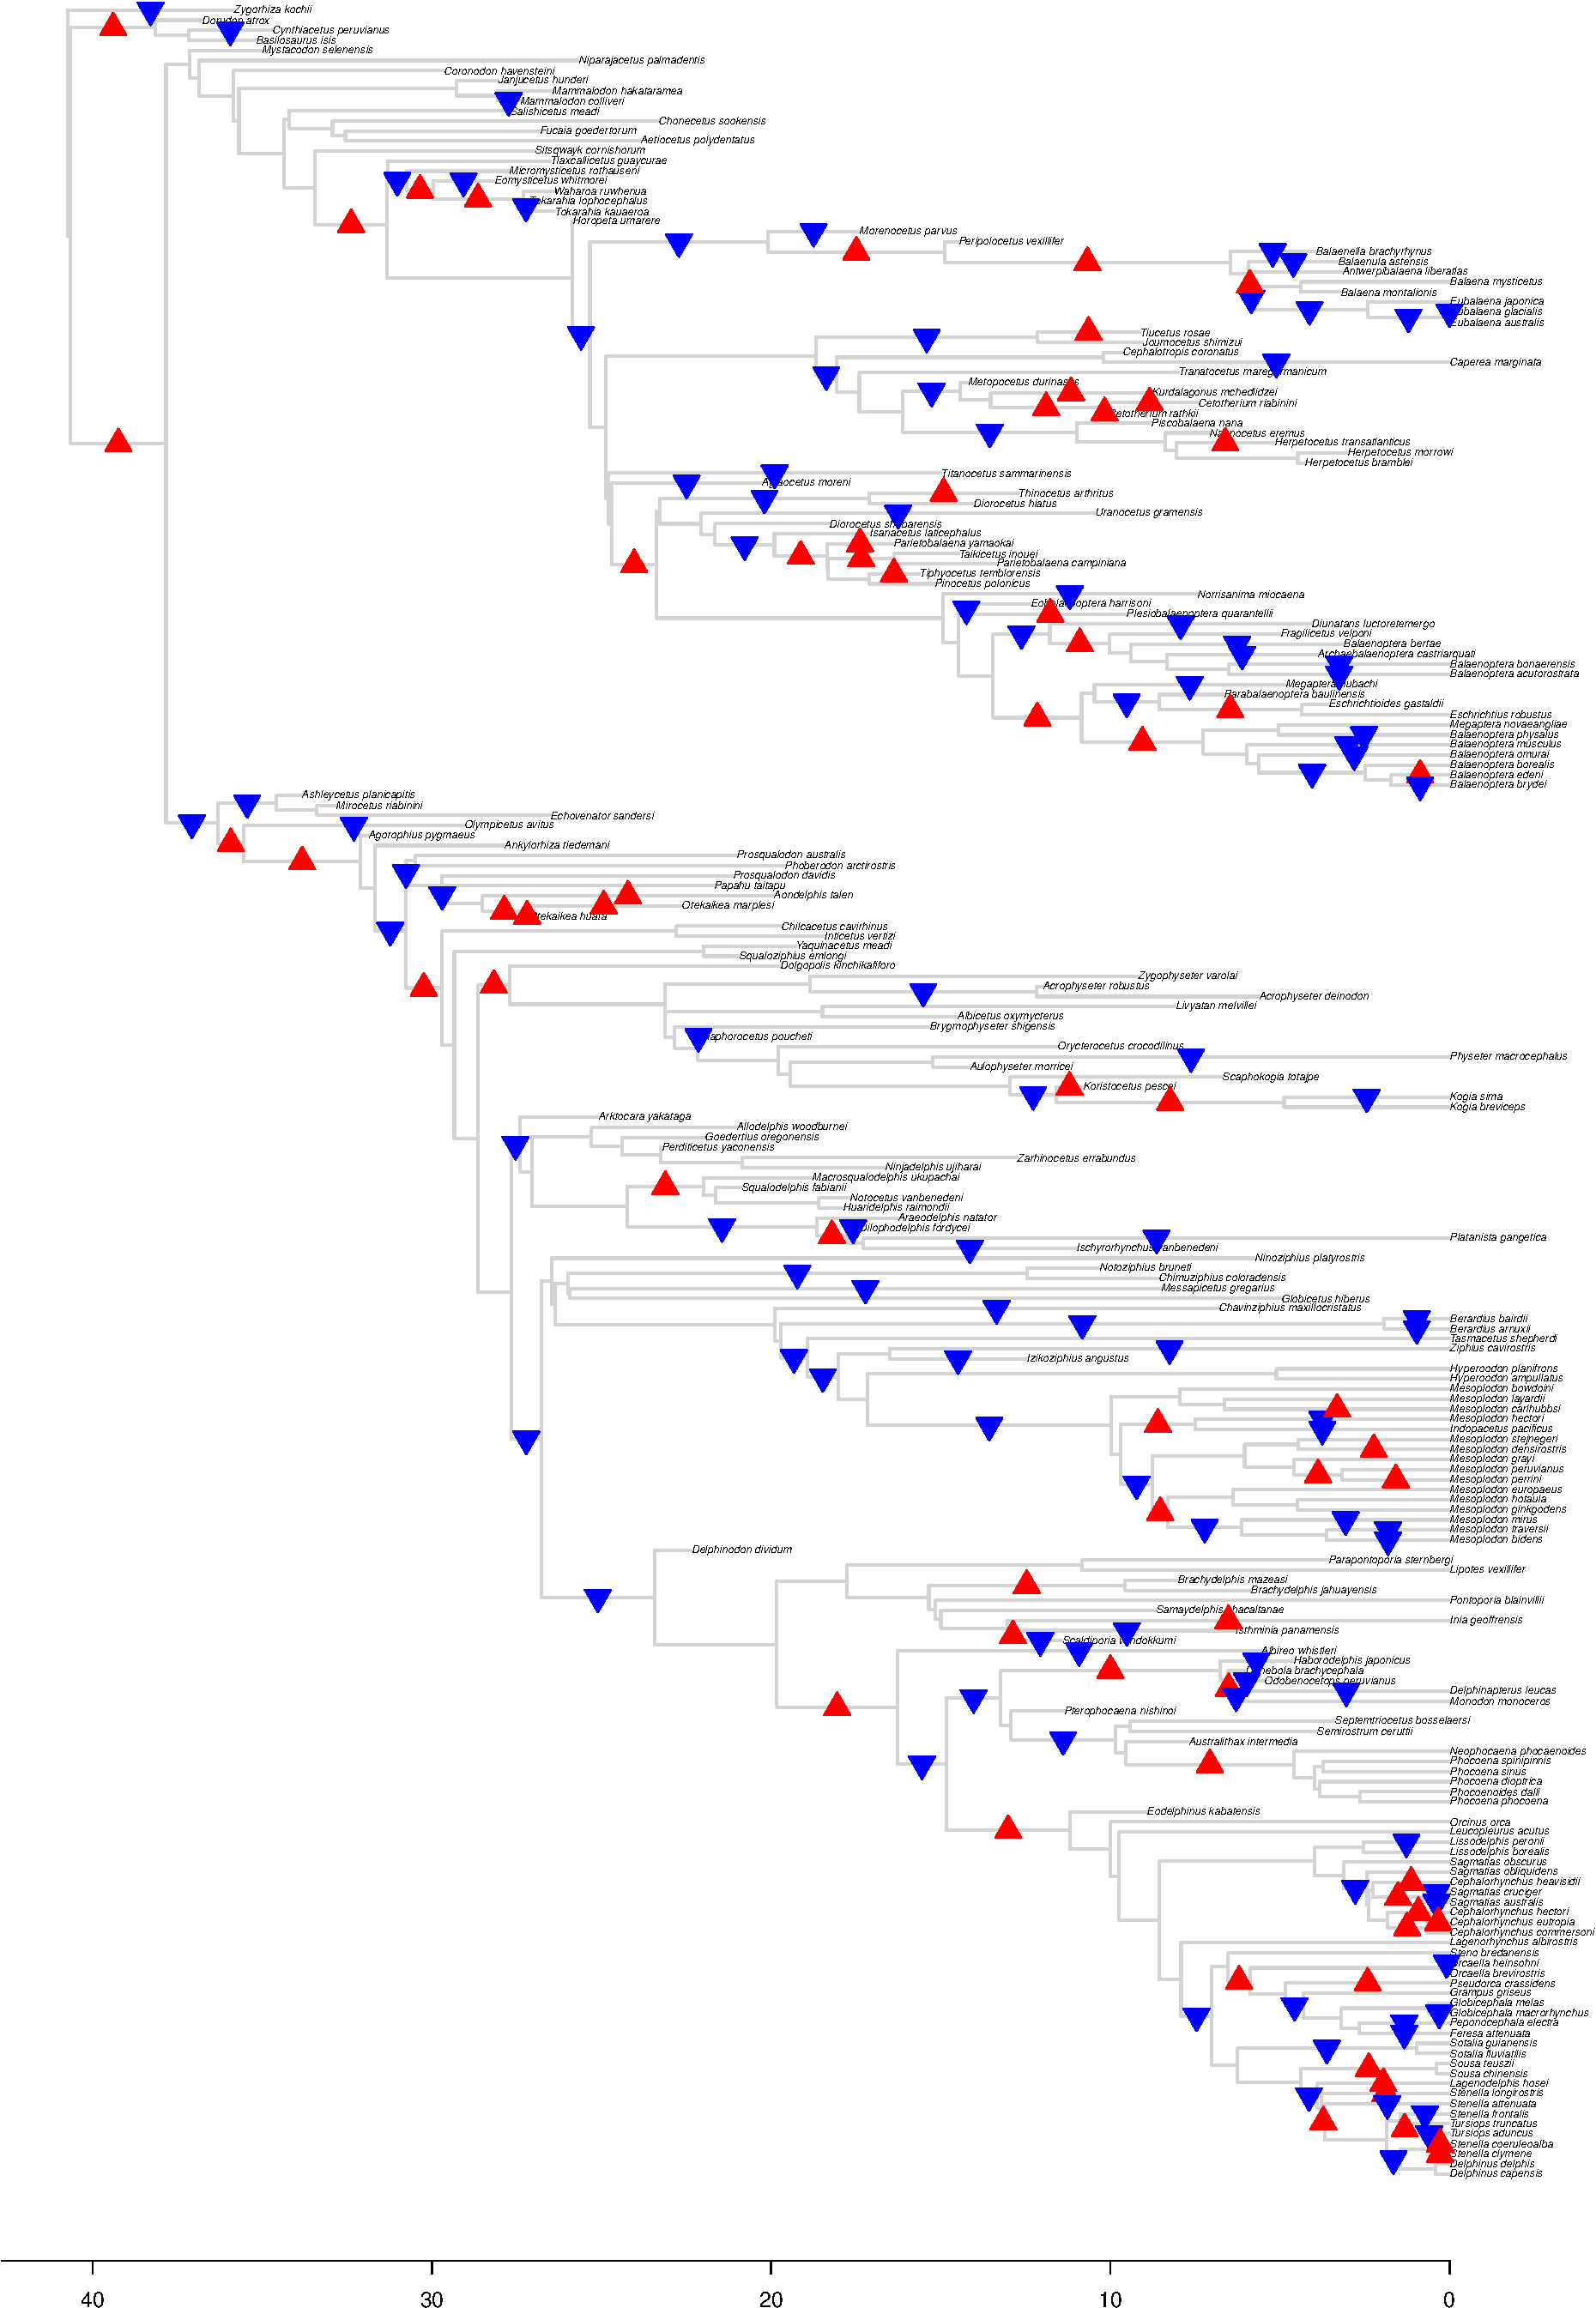
\includegraphics[width=0.9\textwidth]{img/plots-noimput-k50-1.pdf}
\caption{Results for \textit{bayou} fit for the \textit{No Imput} tree, excluding taxa on zero-length branches, setting the average number of shifts in the prior distribution ($\lambda$) to 50. The triangles represent the position and direction of the shifts with posterior probability higher than 0.1, with upward triangles (in red) indicating increases in $\theta$, and downward triangles (in blue) indicating decreases in $\theta$.}
\label{fig:noimput-k50-nzlb}
\end{figure}

\newpage

\begin{figure}[H]
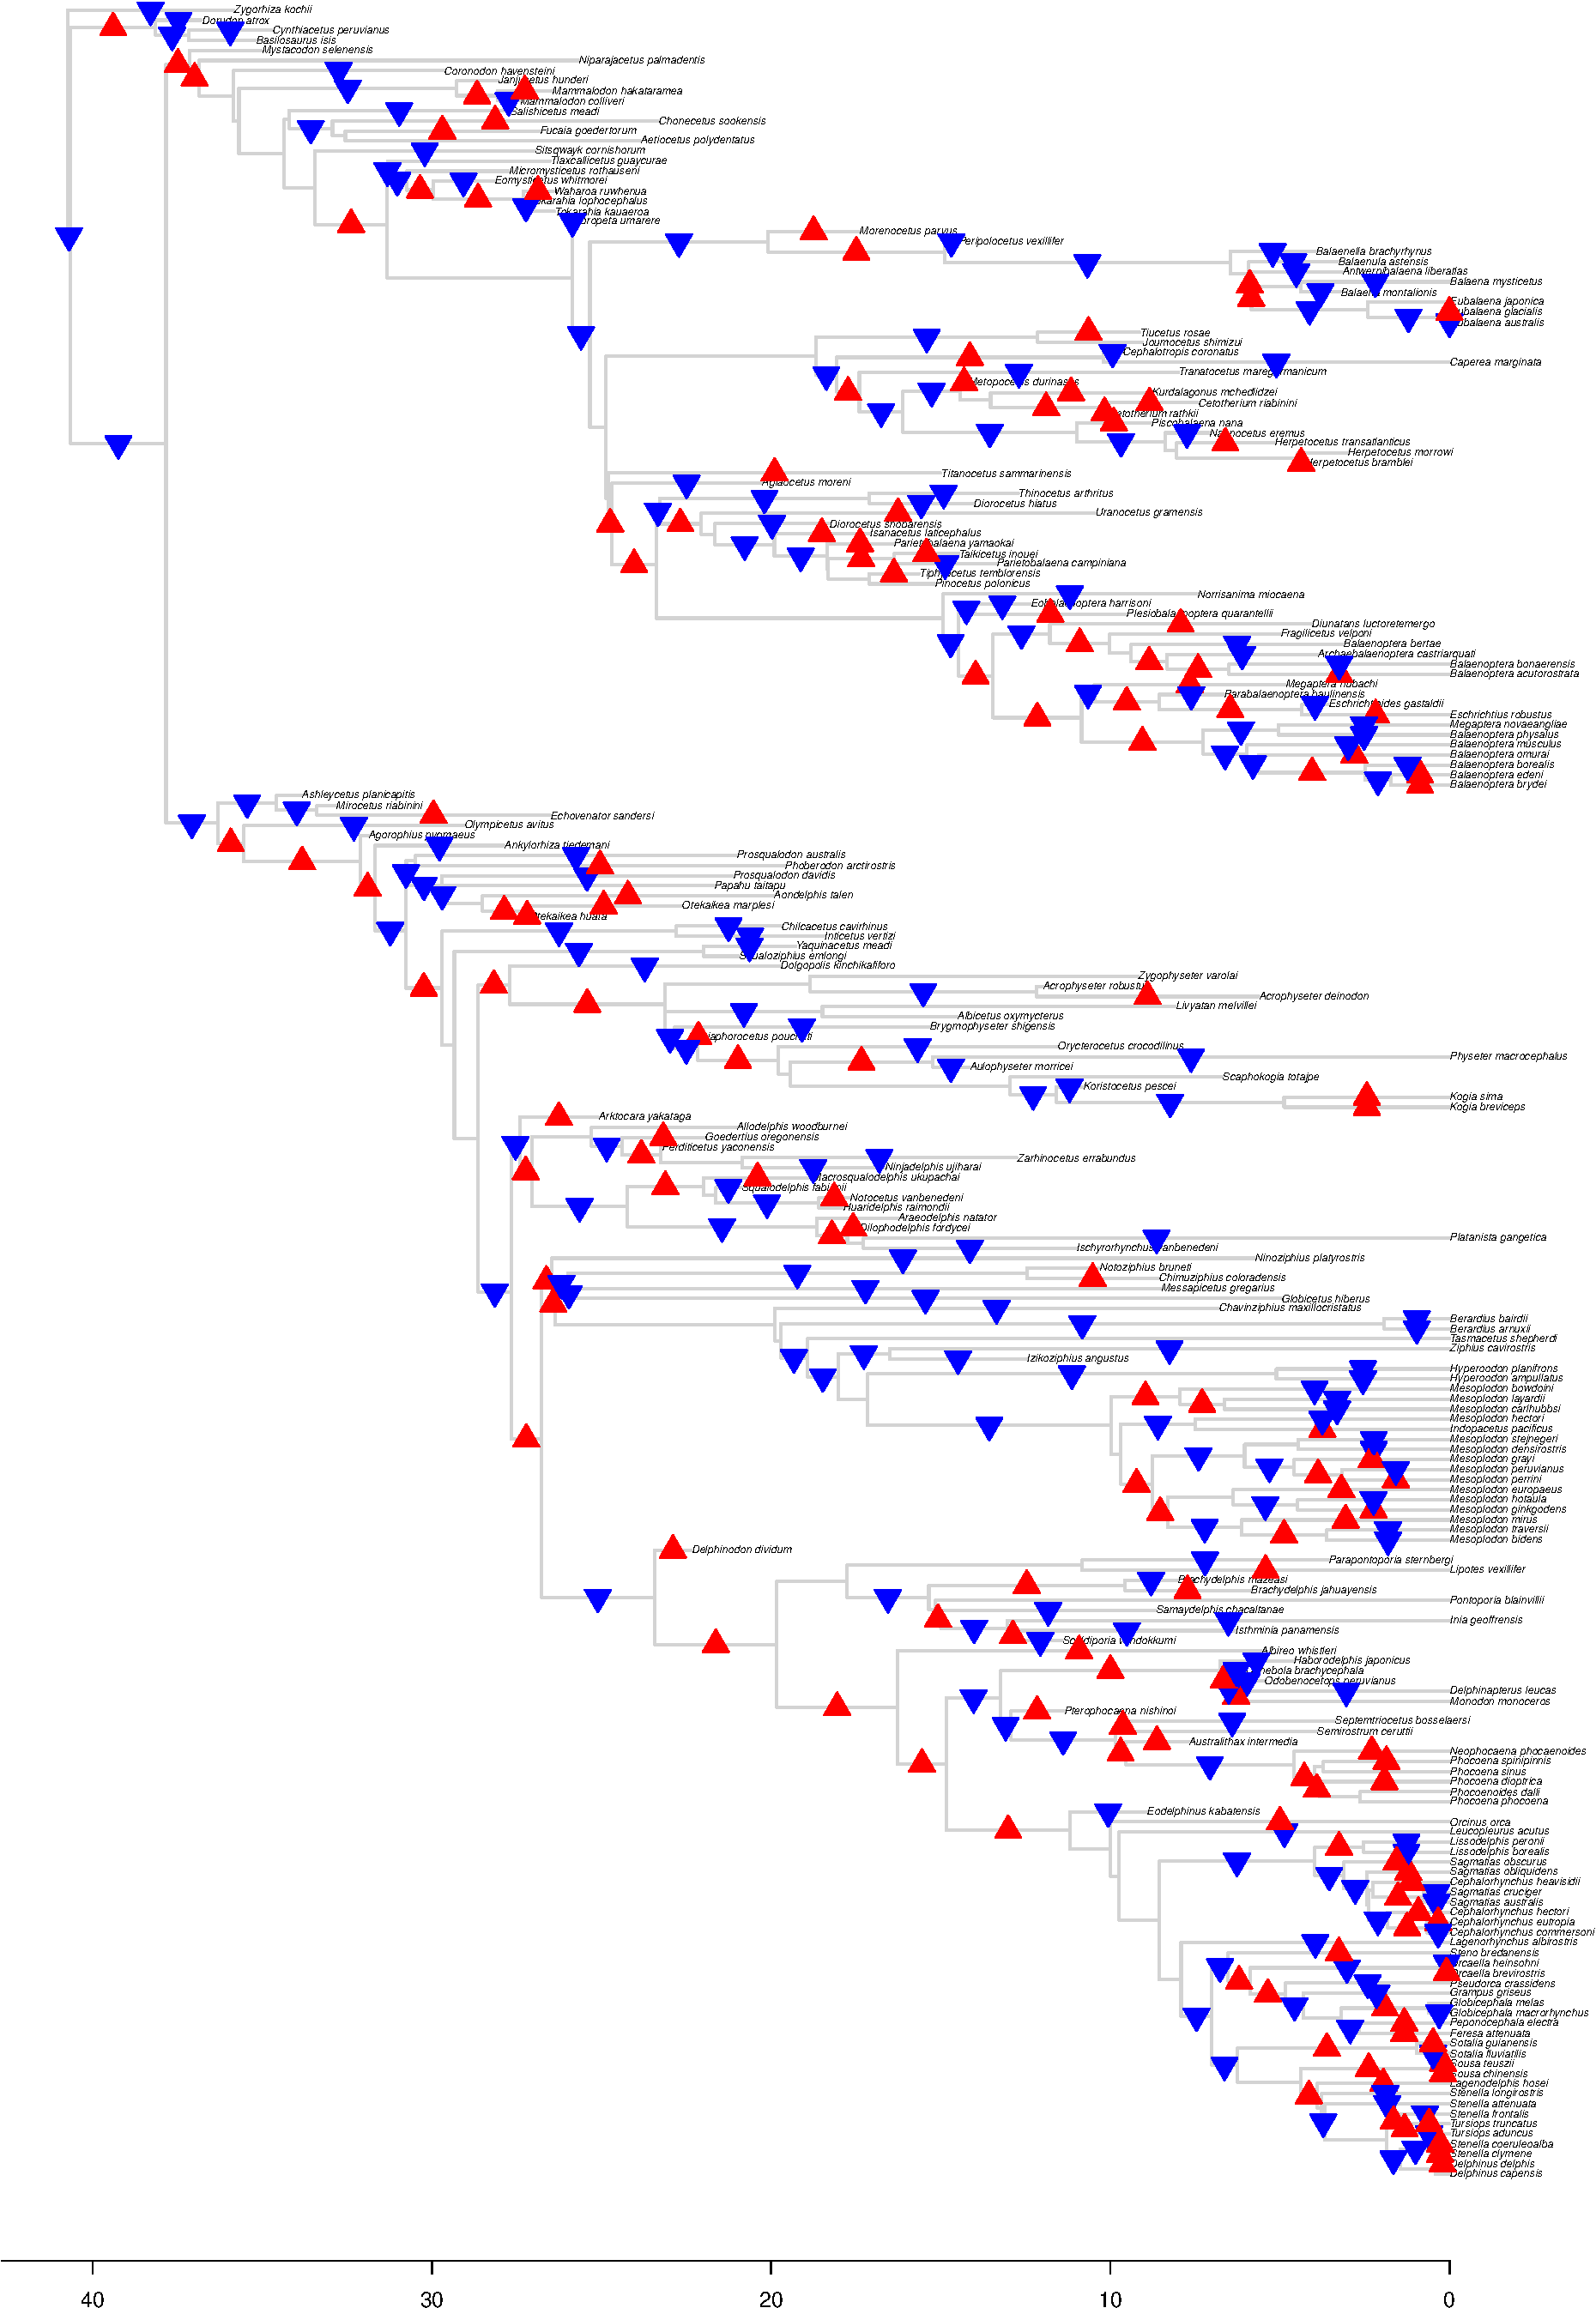
\includegraphics[width=0.9\textwidth]{img/plots-noimput-k250-1.pdf}
\caption{Results for \textit{bayou} fit for the \textit{No Imput} tree, excluding taxa on zero-length branches, setting the average number of shifts in the prior distribution ($\lambda$) to 250. The triangles represent the position and direction of the shifts with posterior probability higher than 0.1, with upward triangles (in red) indicating increases in $\theta$, and downward triangles (in blue) indicating decreases in $\theta$.}
\label{fig:noimput-k250-nzlb}
\end{figure}

\newpage

\begin{figure}[H]
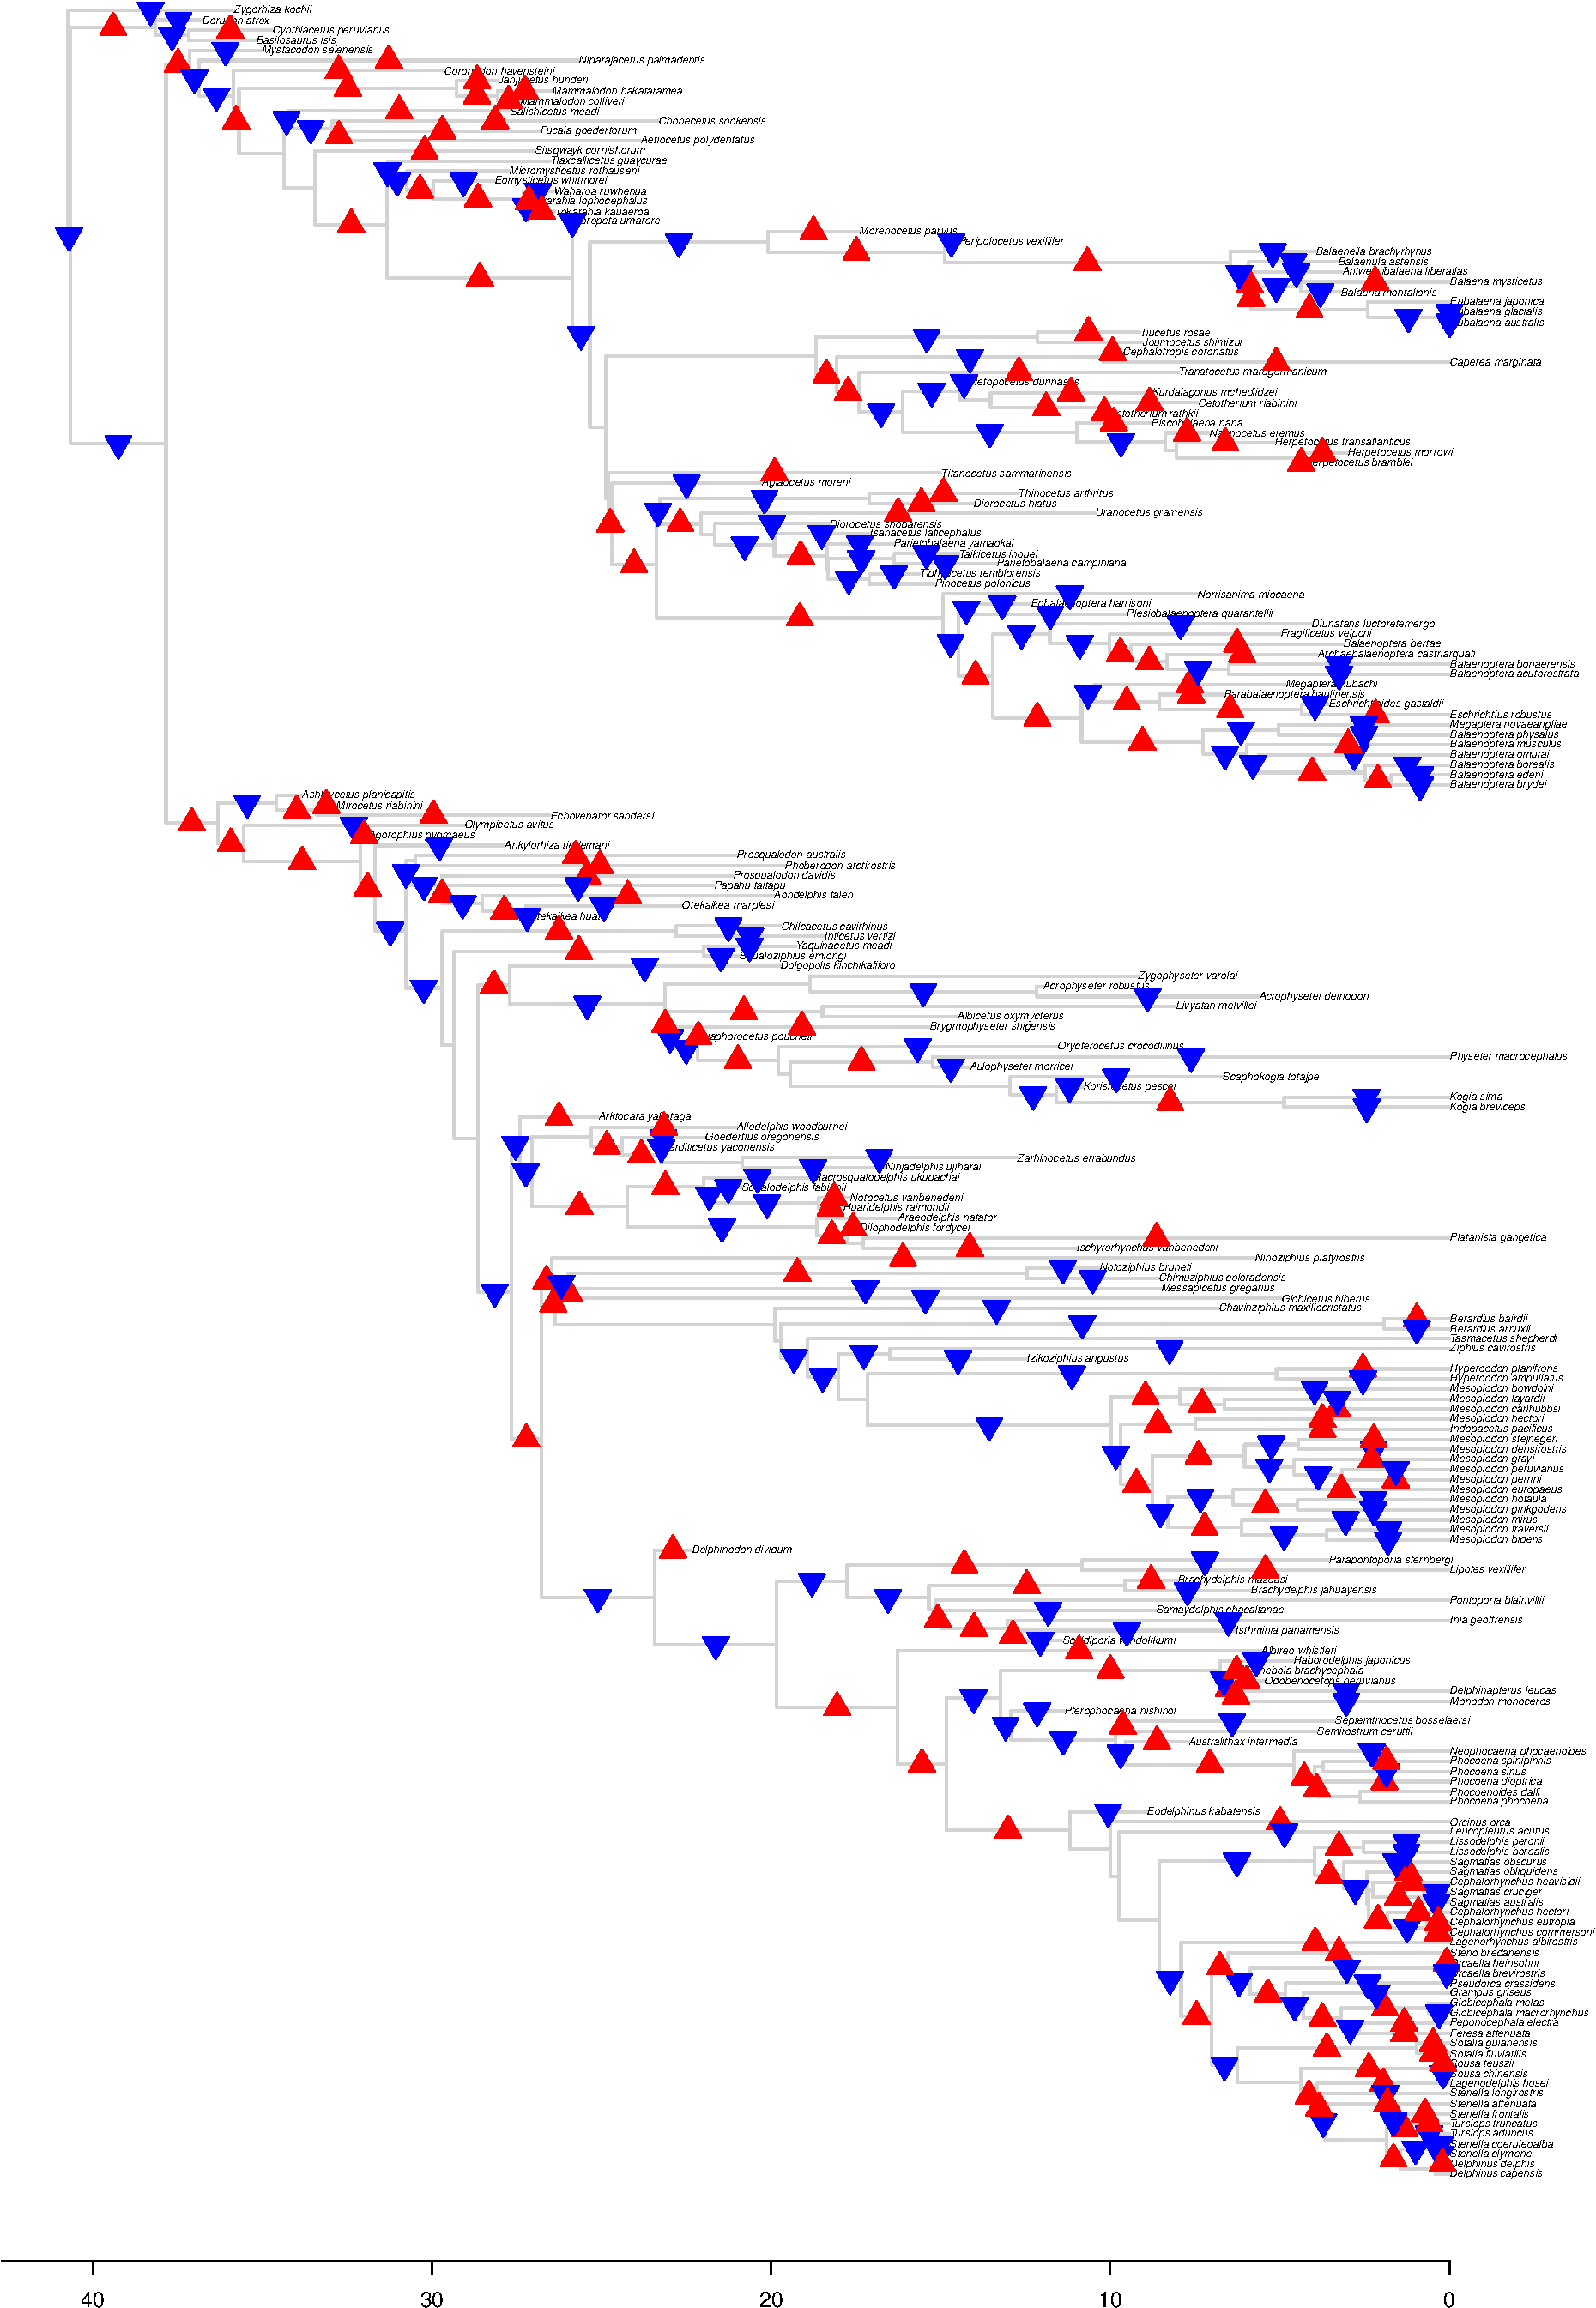
\includegraphics[width=0.9\textwidth]{img/plots-noimput-k500-1.pdf}
\caption{Results for \textit{bayou} fit for the \textit{No Imput} tree, excluding taxa on zero-length branches, setting the average number of shifts in the prior distribution ($\lambda$) to 500. The triangles represent the position and direction of the shifts with posterior probability higher than 0.1, with upward triangles (in red) indicating increases in $\theta$, and downward triangles (in blue) indicating decreases in $\theta$.}
\label{fig:noimput-k500-nzlb}
\end{figure}

%---------------------------------------------------------------------
\subsubsection{\textit{Baleen} tree}
%---------------------------------------------------------------------
\begin{figure}[H]
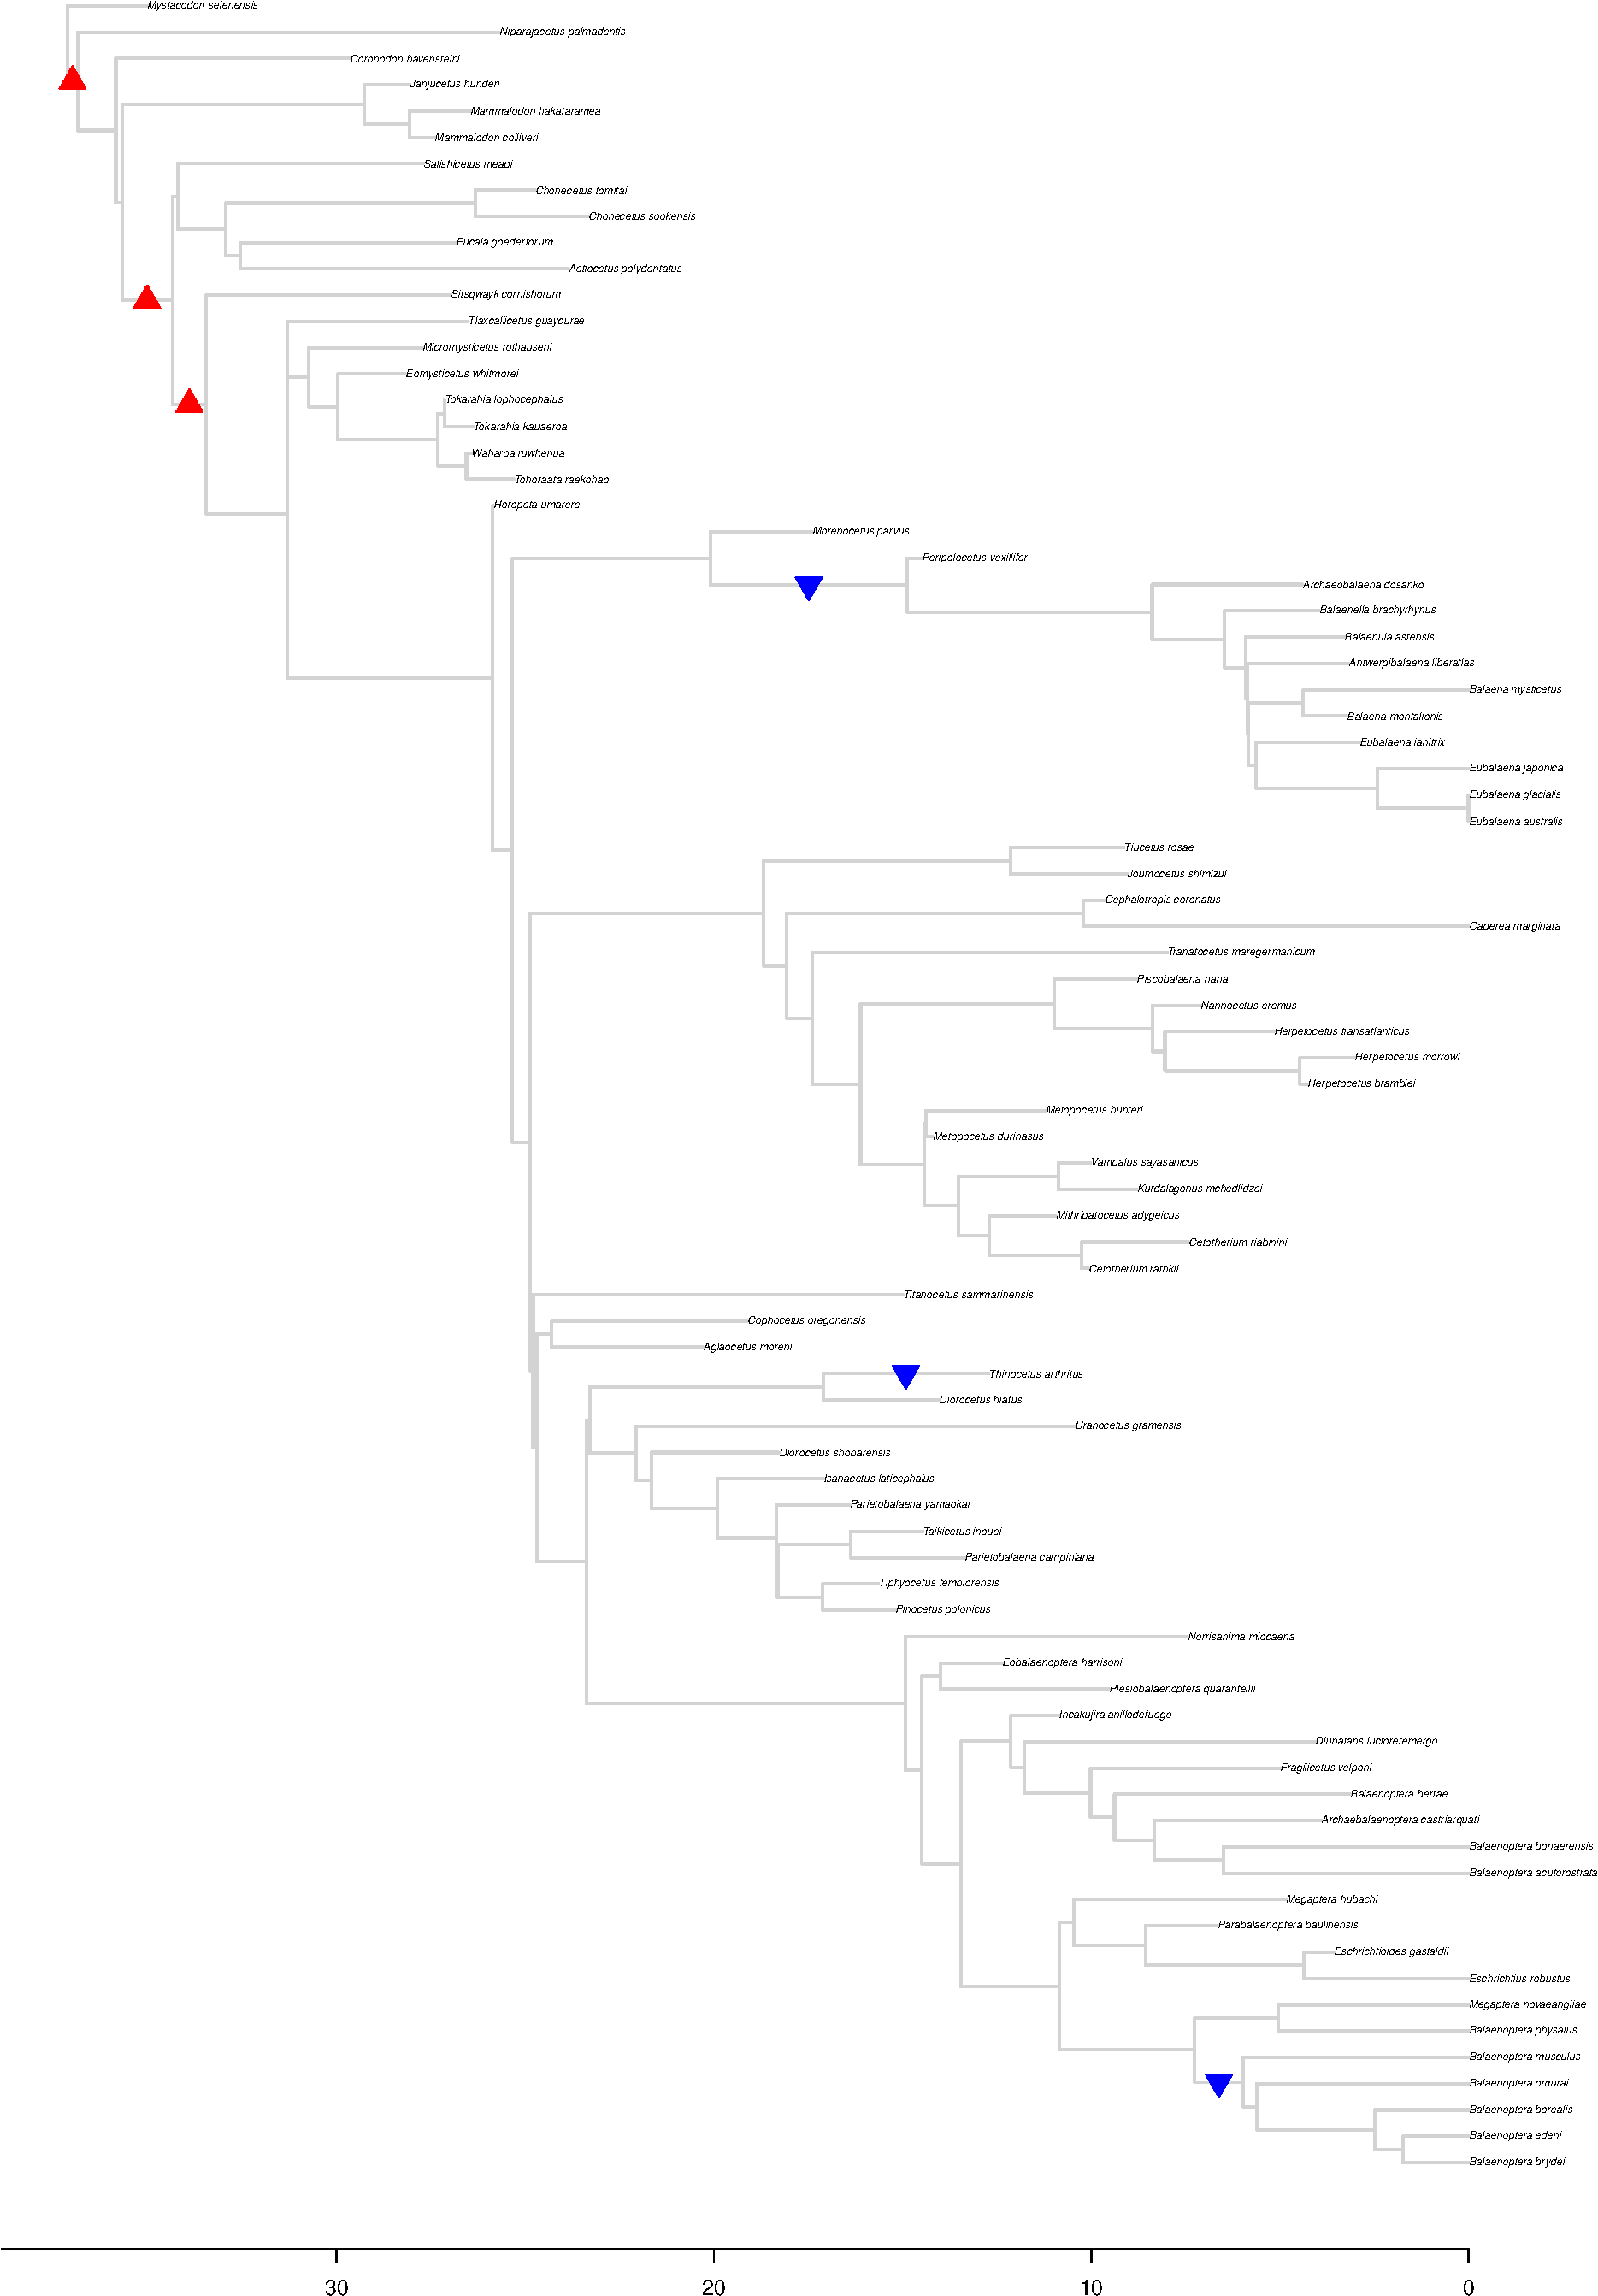
\includegraphics[width=0.9\textwidth]{img/plots-baleen-k5-1.pdf}
\caption{Results for \textit{bayou} fit for the \textit{Baleen} tree, excluding taxa on zero-length branches, setting the average number of shifts in the prior distribution ($\lambda$) to 5. The triangles represent the position and direction of the shifts with posterior probability higher than 0.1, with upward triangles (in red) indicating increases in $\theta$, and downward triangles (in blue) indicating decreases in $\theta$.}
\label{fig:baleen-k5-nzlb}
\end{figure}

\newpage

\begin{figure}[H]
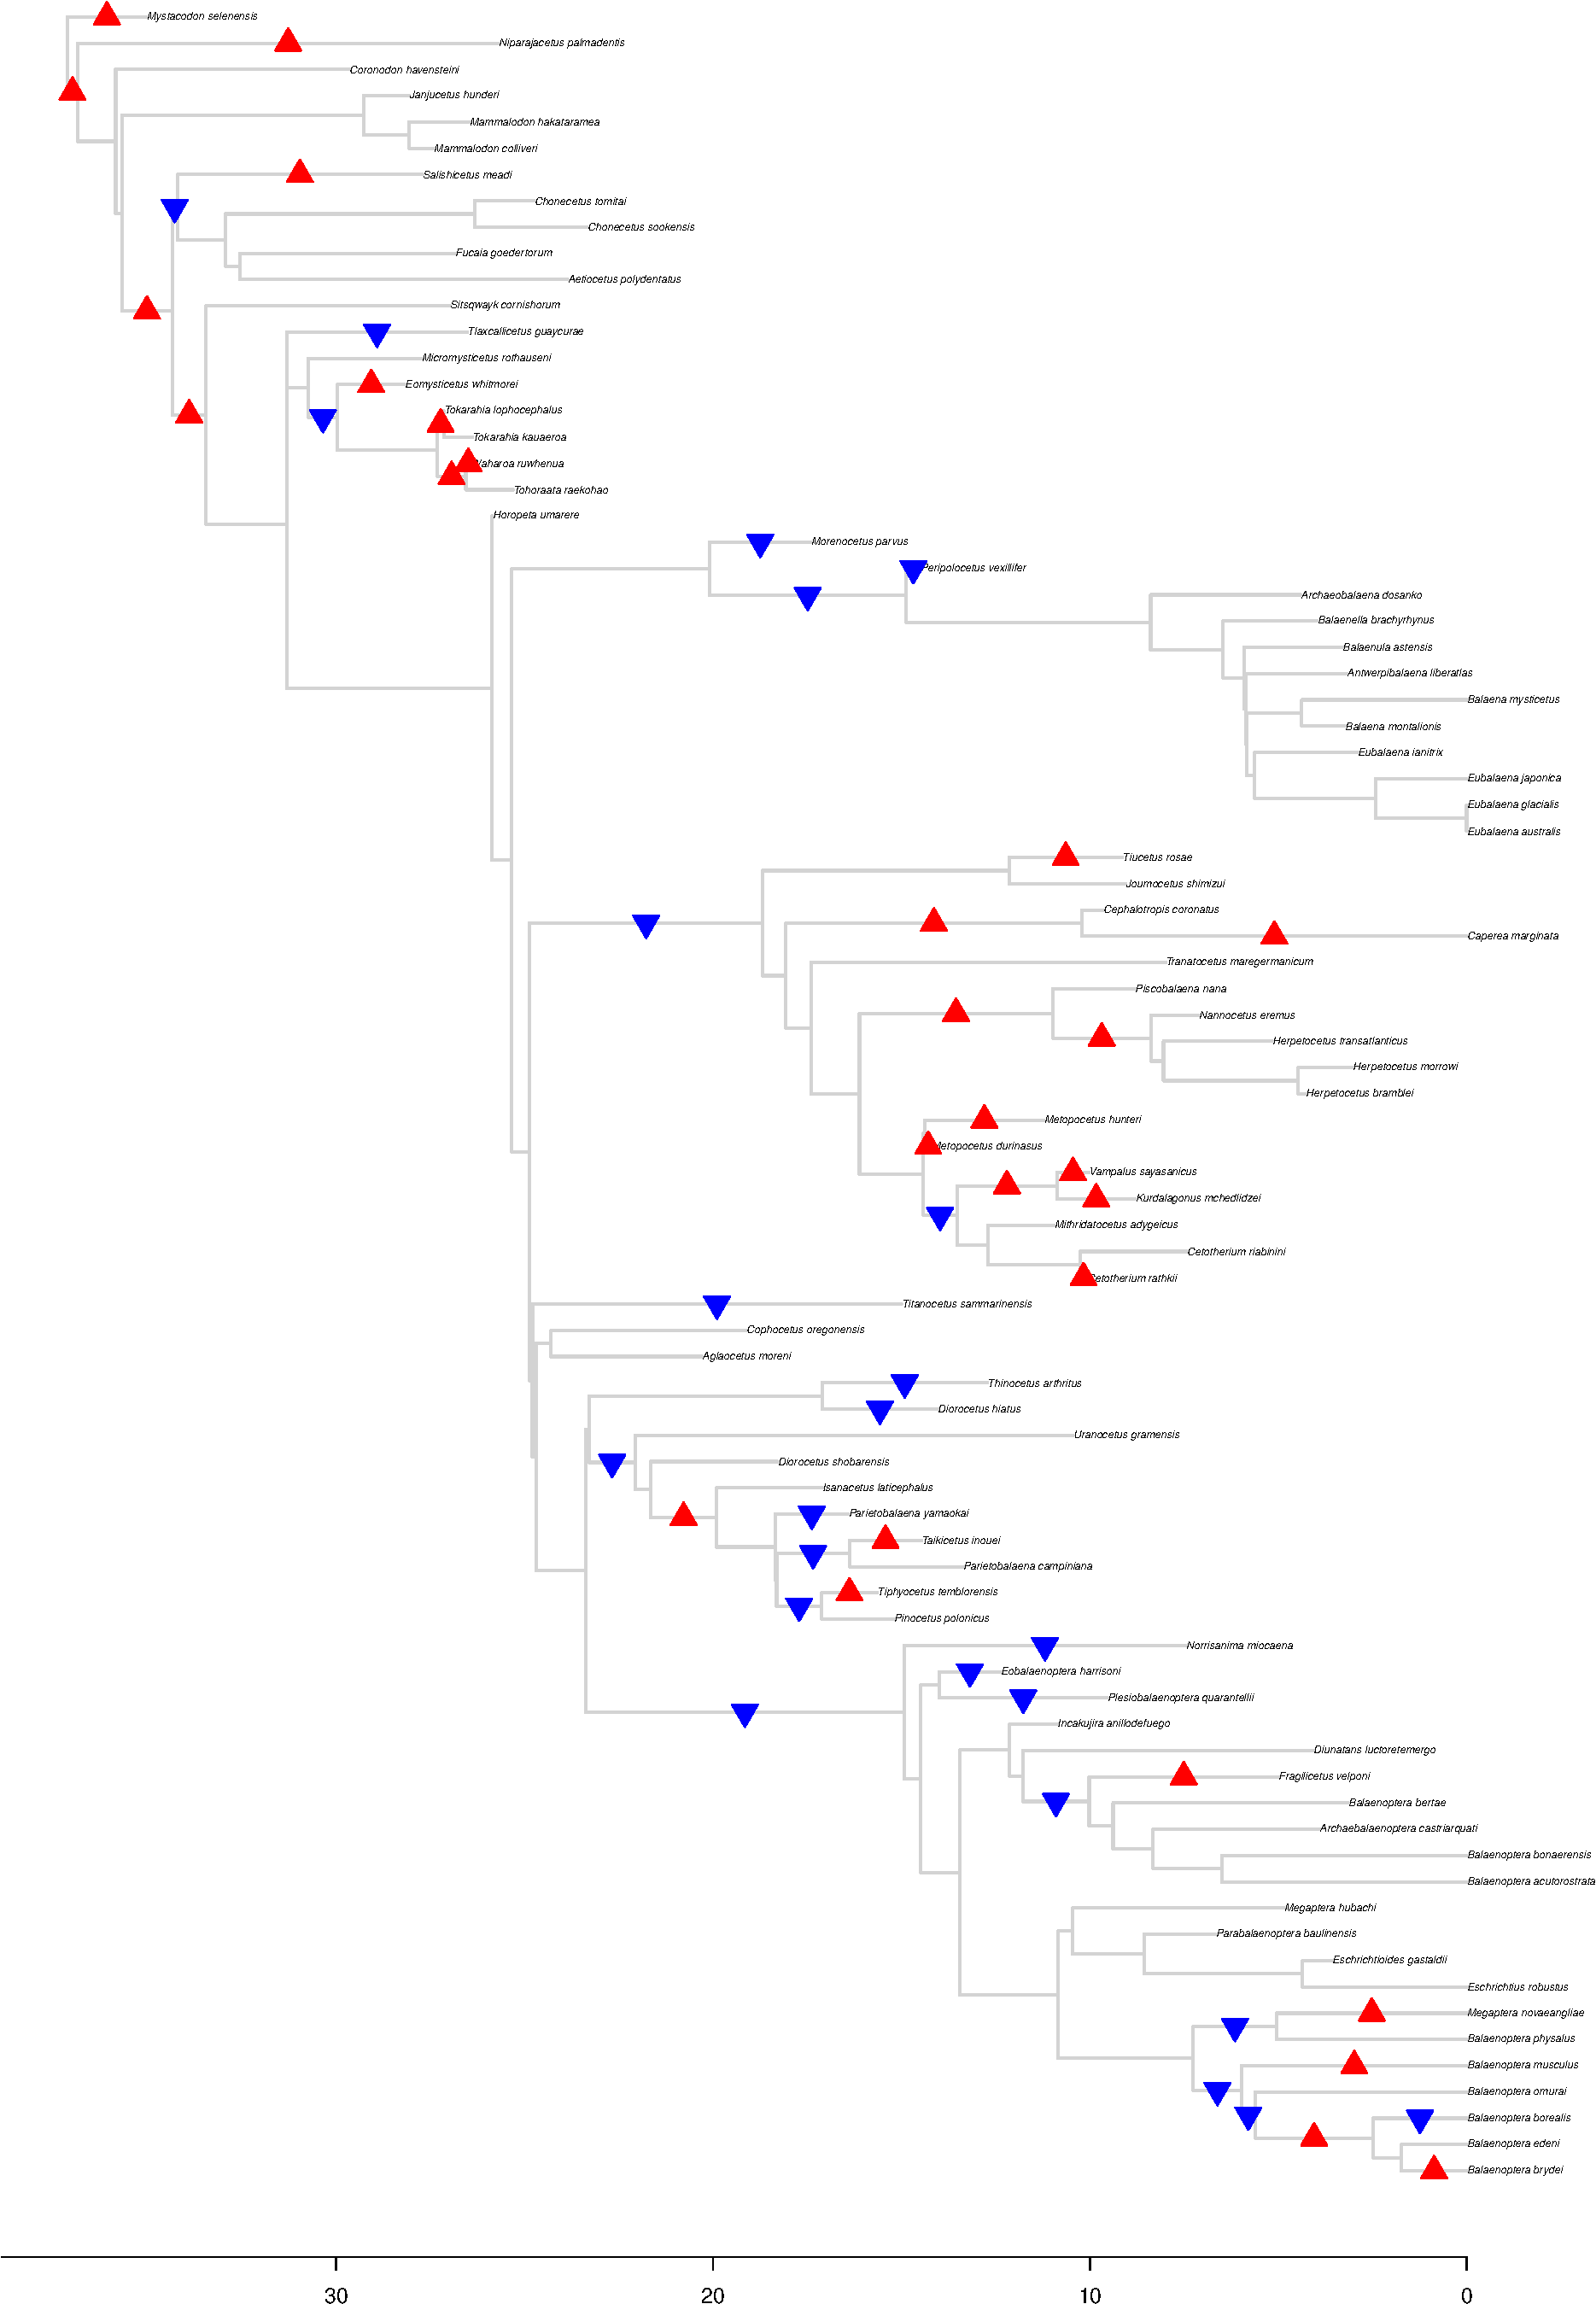
\includegraphics[width=0.9\textwidth]{img/plots-baleen-k15-1.pdf}
\caption{Results for \textit{bayou} fit for the \textit{Baleen} tree, excluding taxa on zero-length branches, setting the average number of shifts in the prior distribution ($\lambda$) to 15. The triangles represent the position and direction of the shifts with posterior probability higher than 0.1, with upward triangles (in red) indicating increases in $\theta$, and downward triangles (in blue) indicating decreases in $\theta$.}
\label{fig:baleen-k15-nzlb}
\end{figure}

\newpage

\begin{figure}[H]
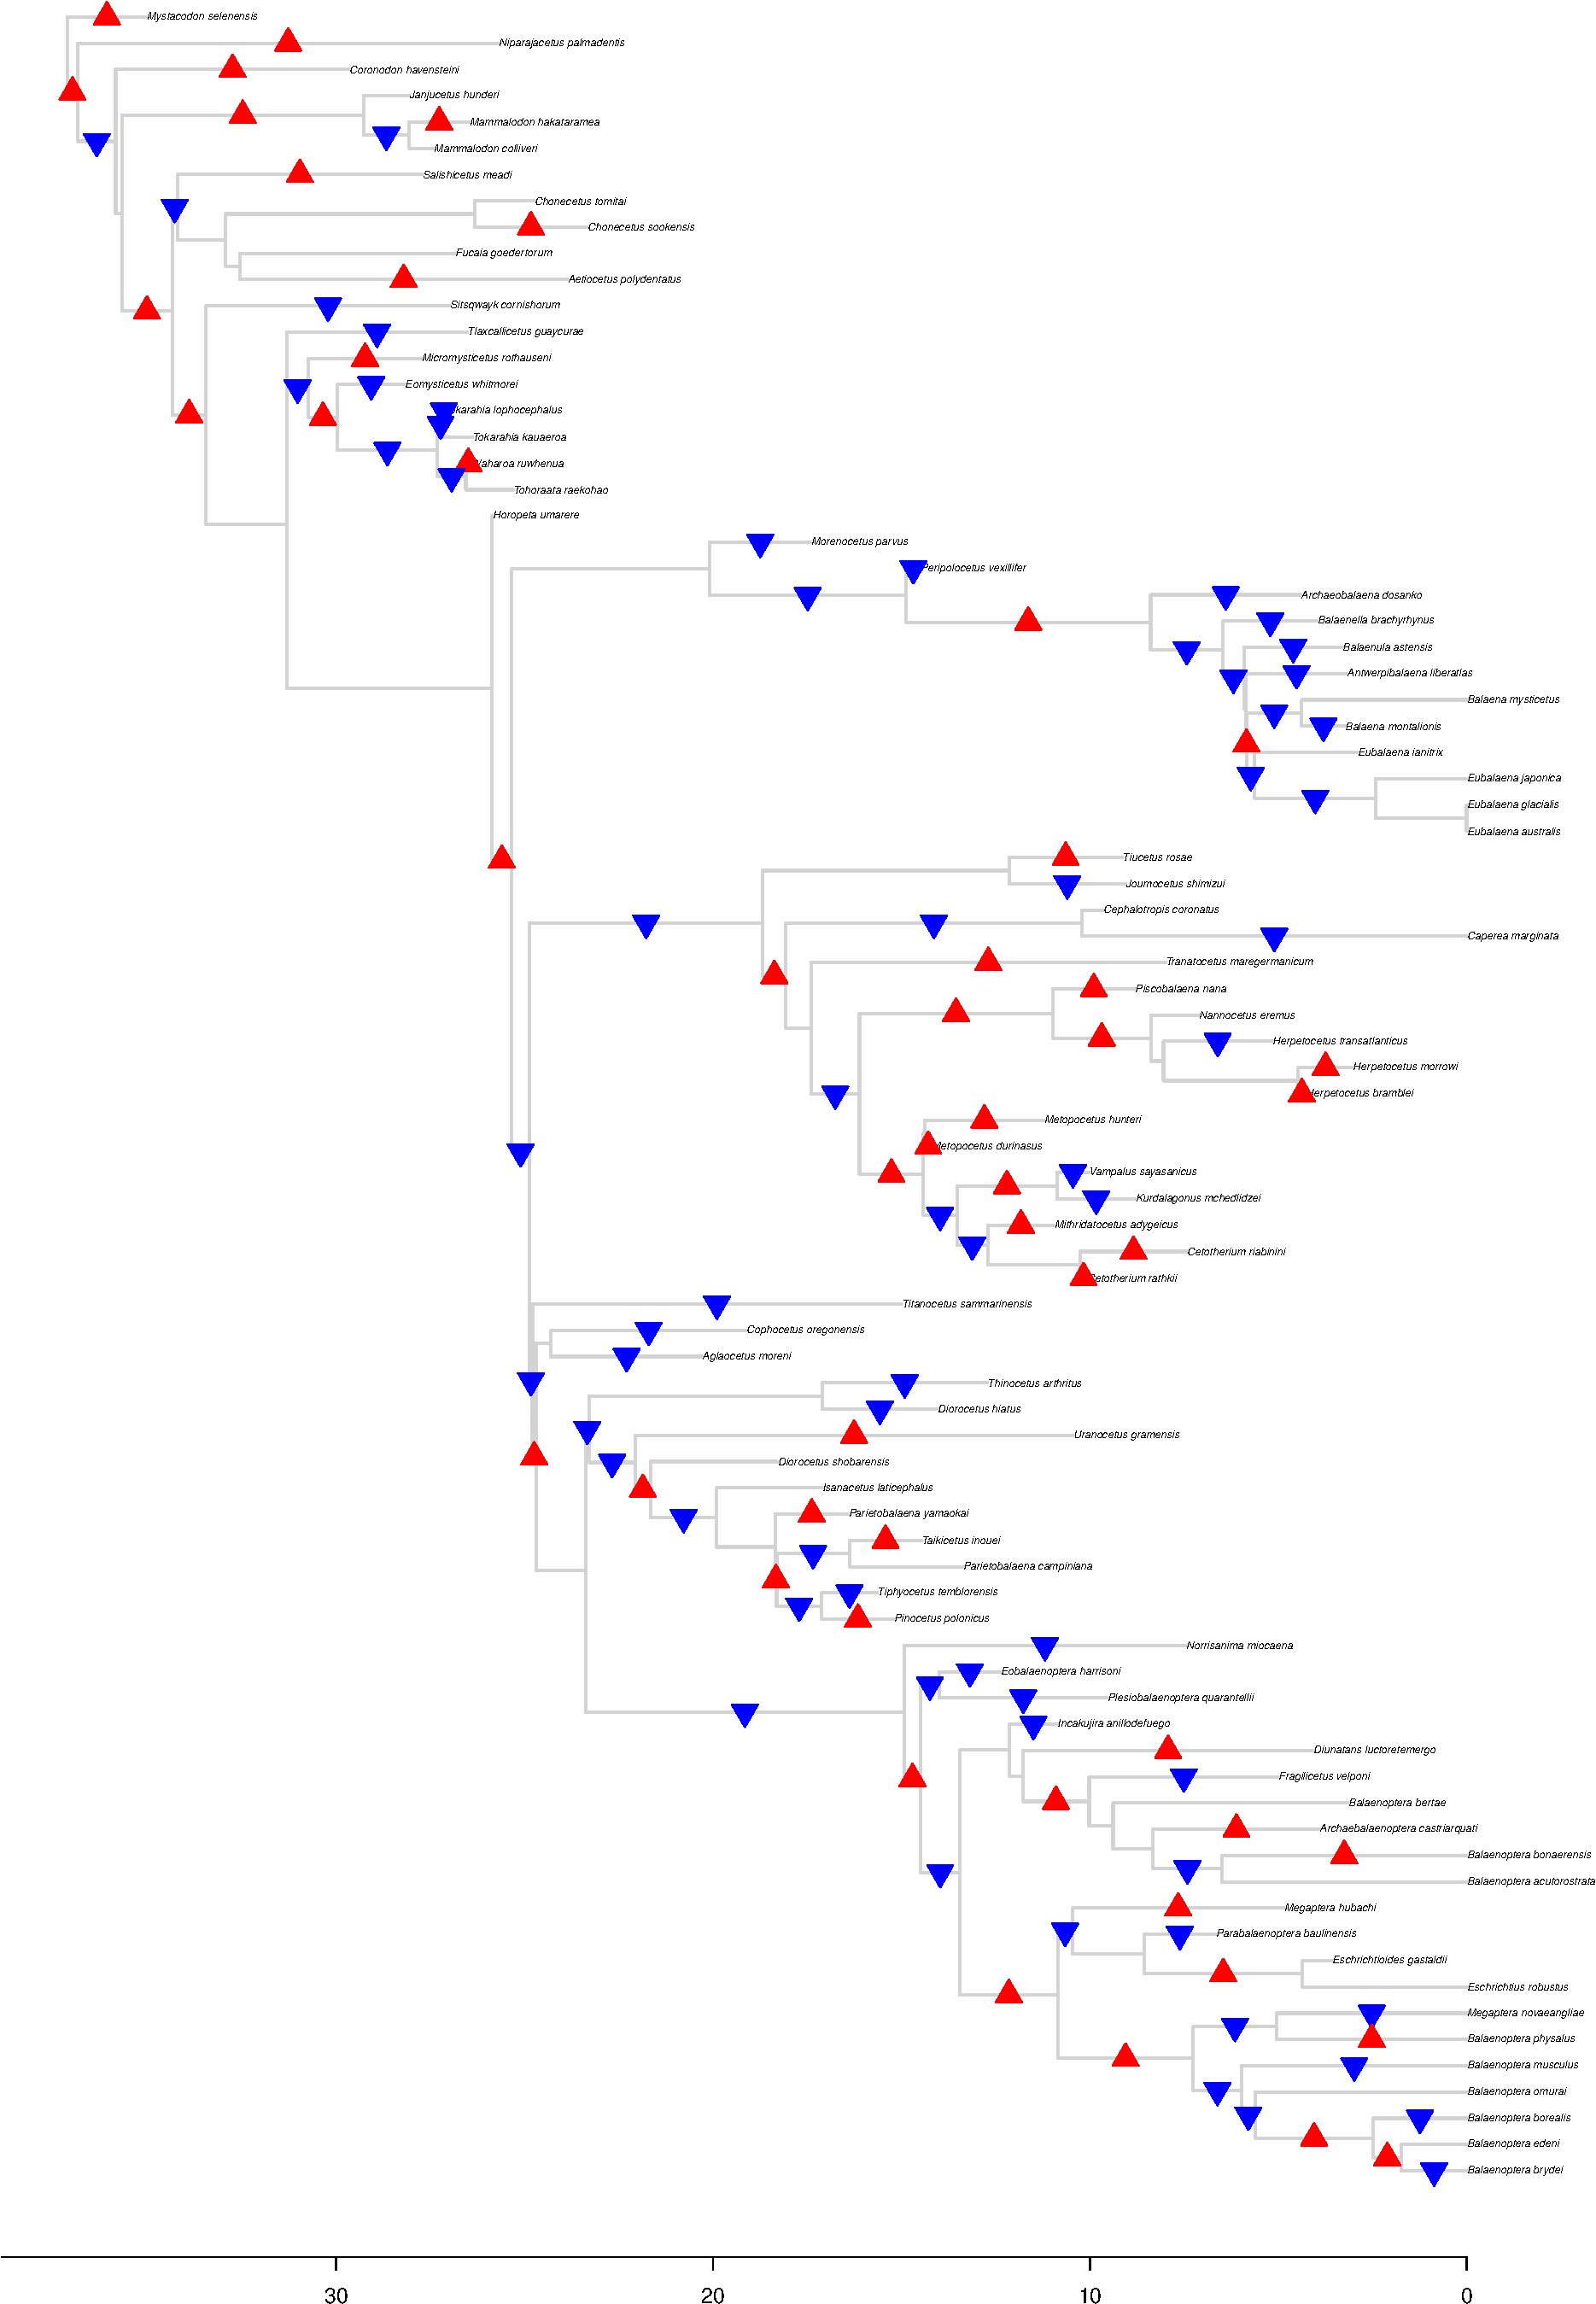
\includegraphics[width=0.9\textwidth]{img/plots-baleen-k50-1.pdf}
\caption{Results for \textit{bayou} fit for the \textit{Baleen} tree, excluding taxa on zero-length branches, setting the average number of shifts in the prior distribution ($\lambda$) to 50. The triangles represent the position and direction of the shifts with posterior probability higher than 0.1, with upward triangles (in red) indicating increases in $\theta$, and downward triangles (in blue) indicating decreases in $\theta$.}
\label{fig:baleen-k50-nzlb}
\end{figure}

\newpage
%---------------------------------------------------------------------
\subsubsection{\textit{Toothed} tree}
%---------------------------------------------------------------------

\begin{figure}[H]
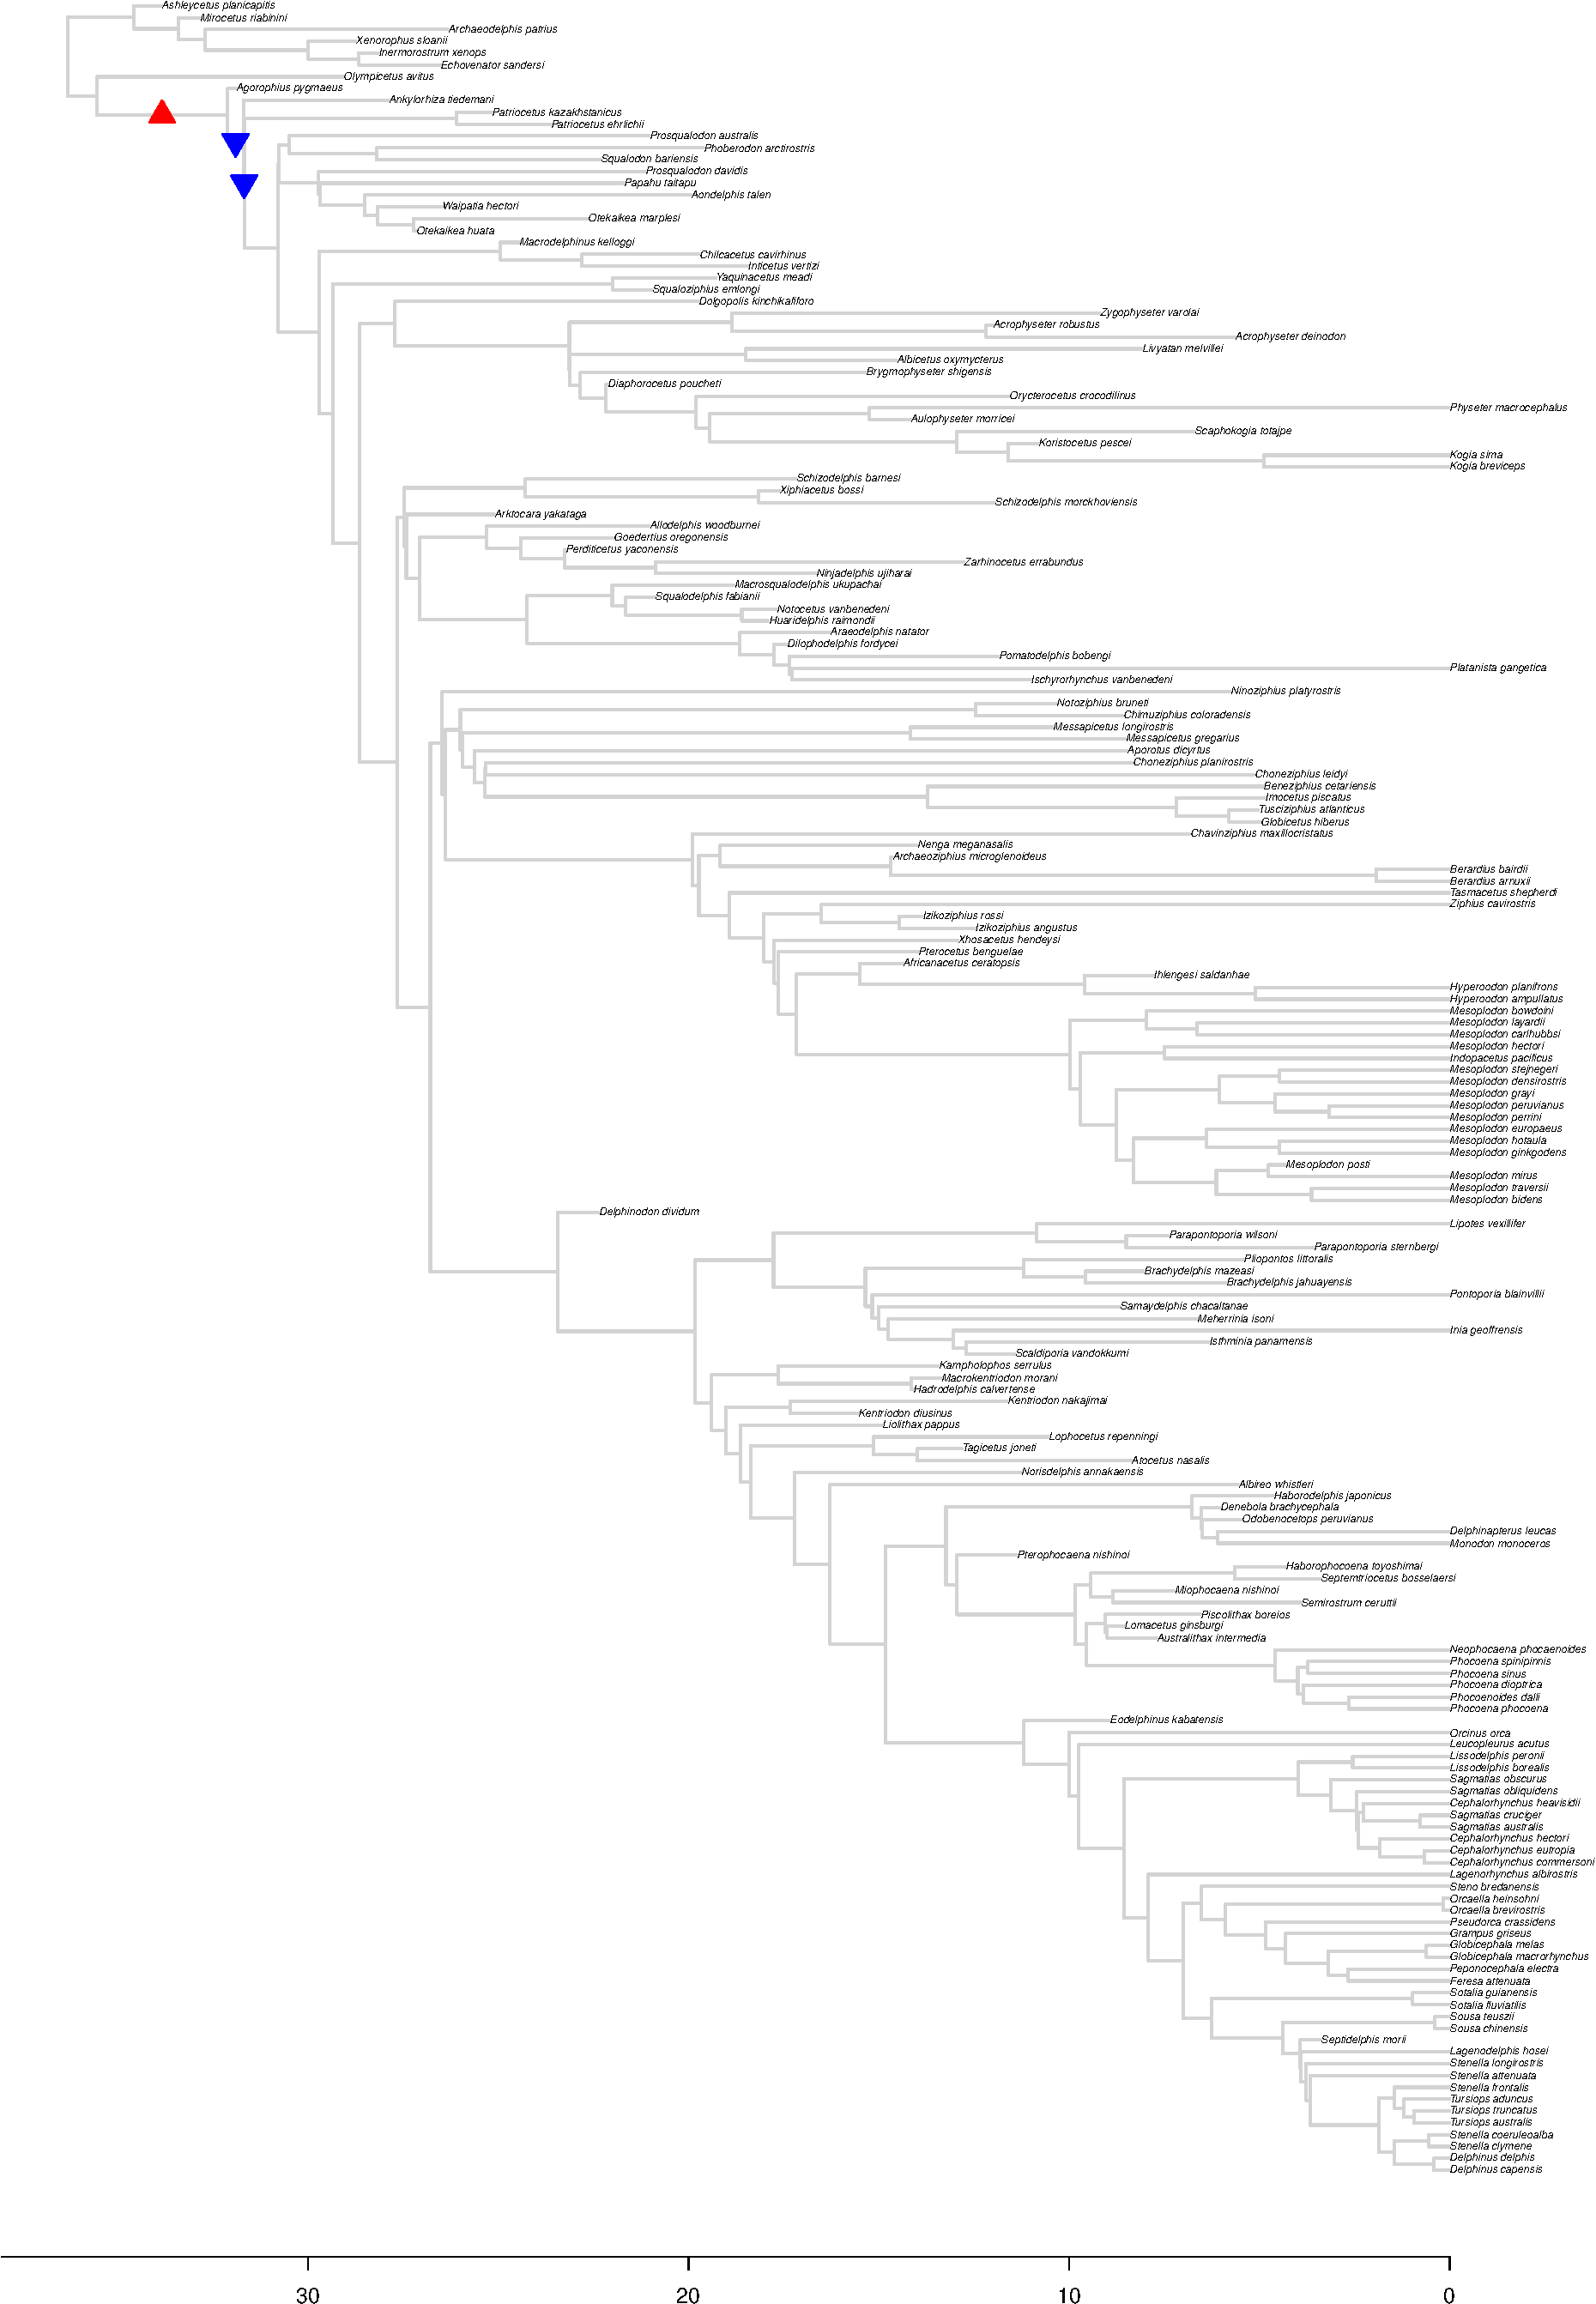
\includegraphics[width=0.9\textwidth]{img/plots-toothed-k5-1.pdf}
\caption{Results for \textit{bayou} fit for the \textit{Toothed} tree, excluding taxa on zero-length branches, setting the average number of shifts in the prior distribution ($\lambda$) to 5. The triangles represent the position and direction of the shifts with posterior probability higher than 0.1, with upward triangles (in red) indicating increases in $\theta$, and downward triangles (in blue) indicating decreases in $\theta$.}
\label{fig:toothed-k5-nzlb}
\end{figure}

\newpage

\begin{figure}[H]
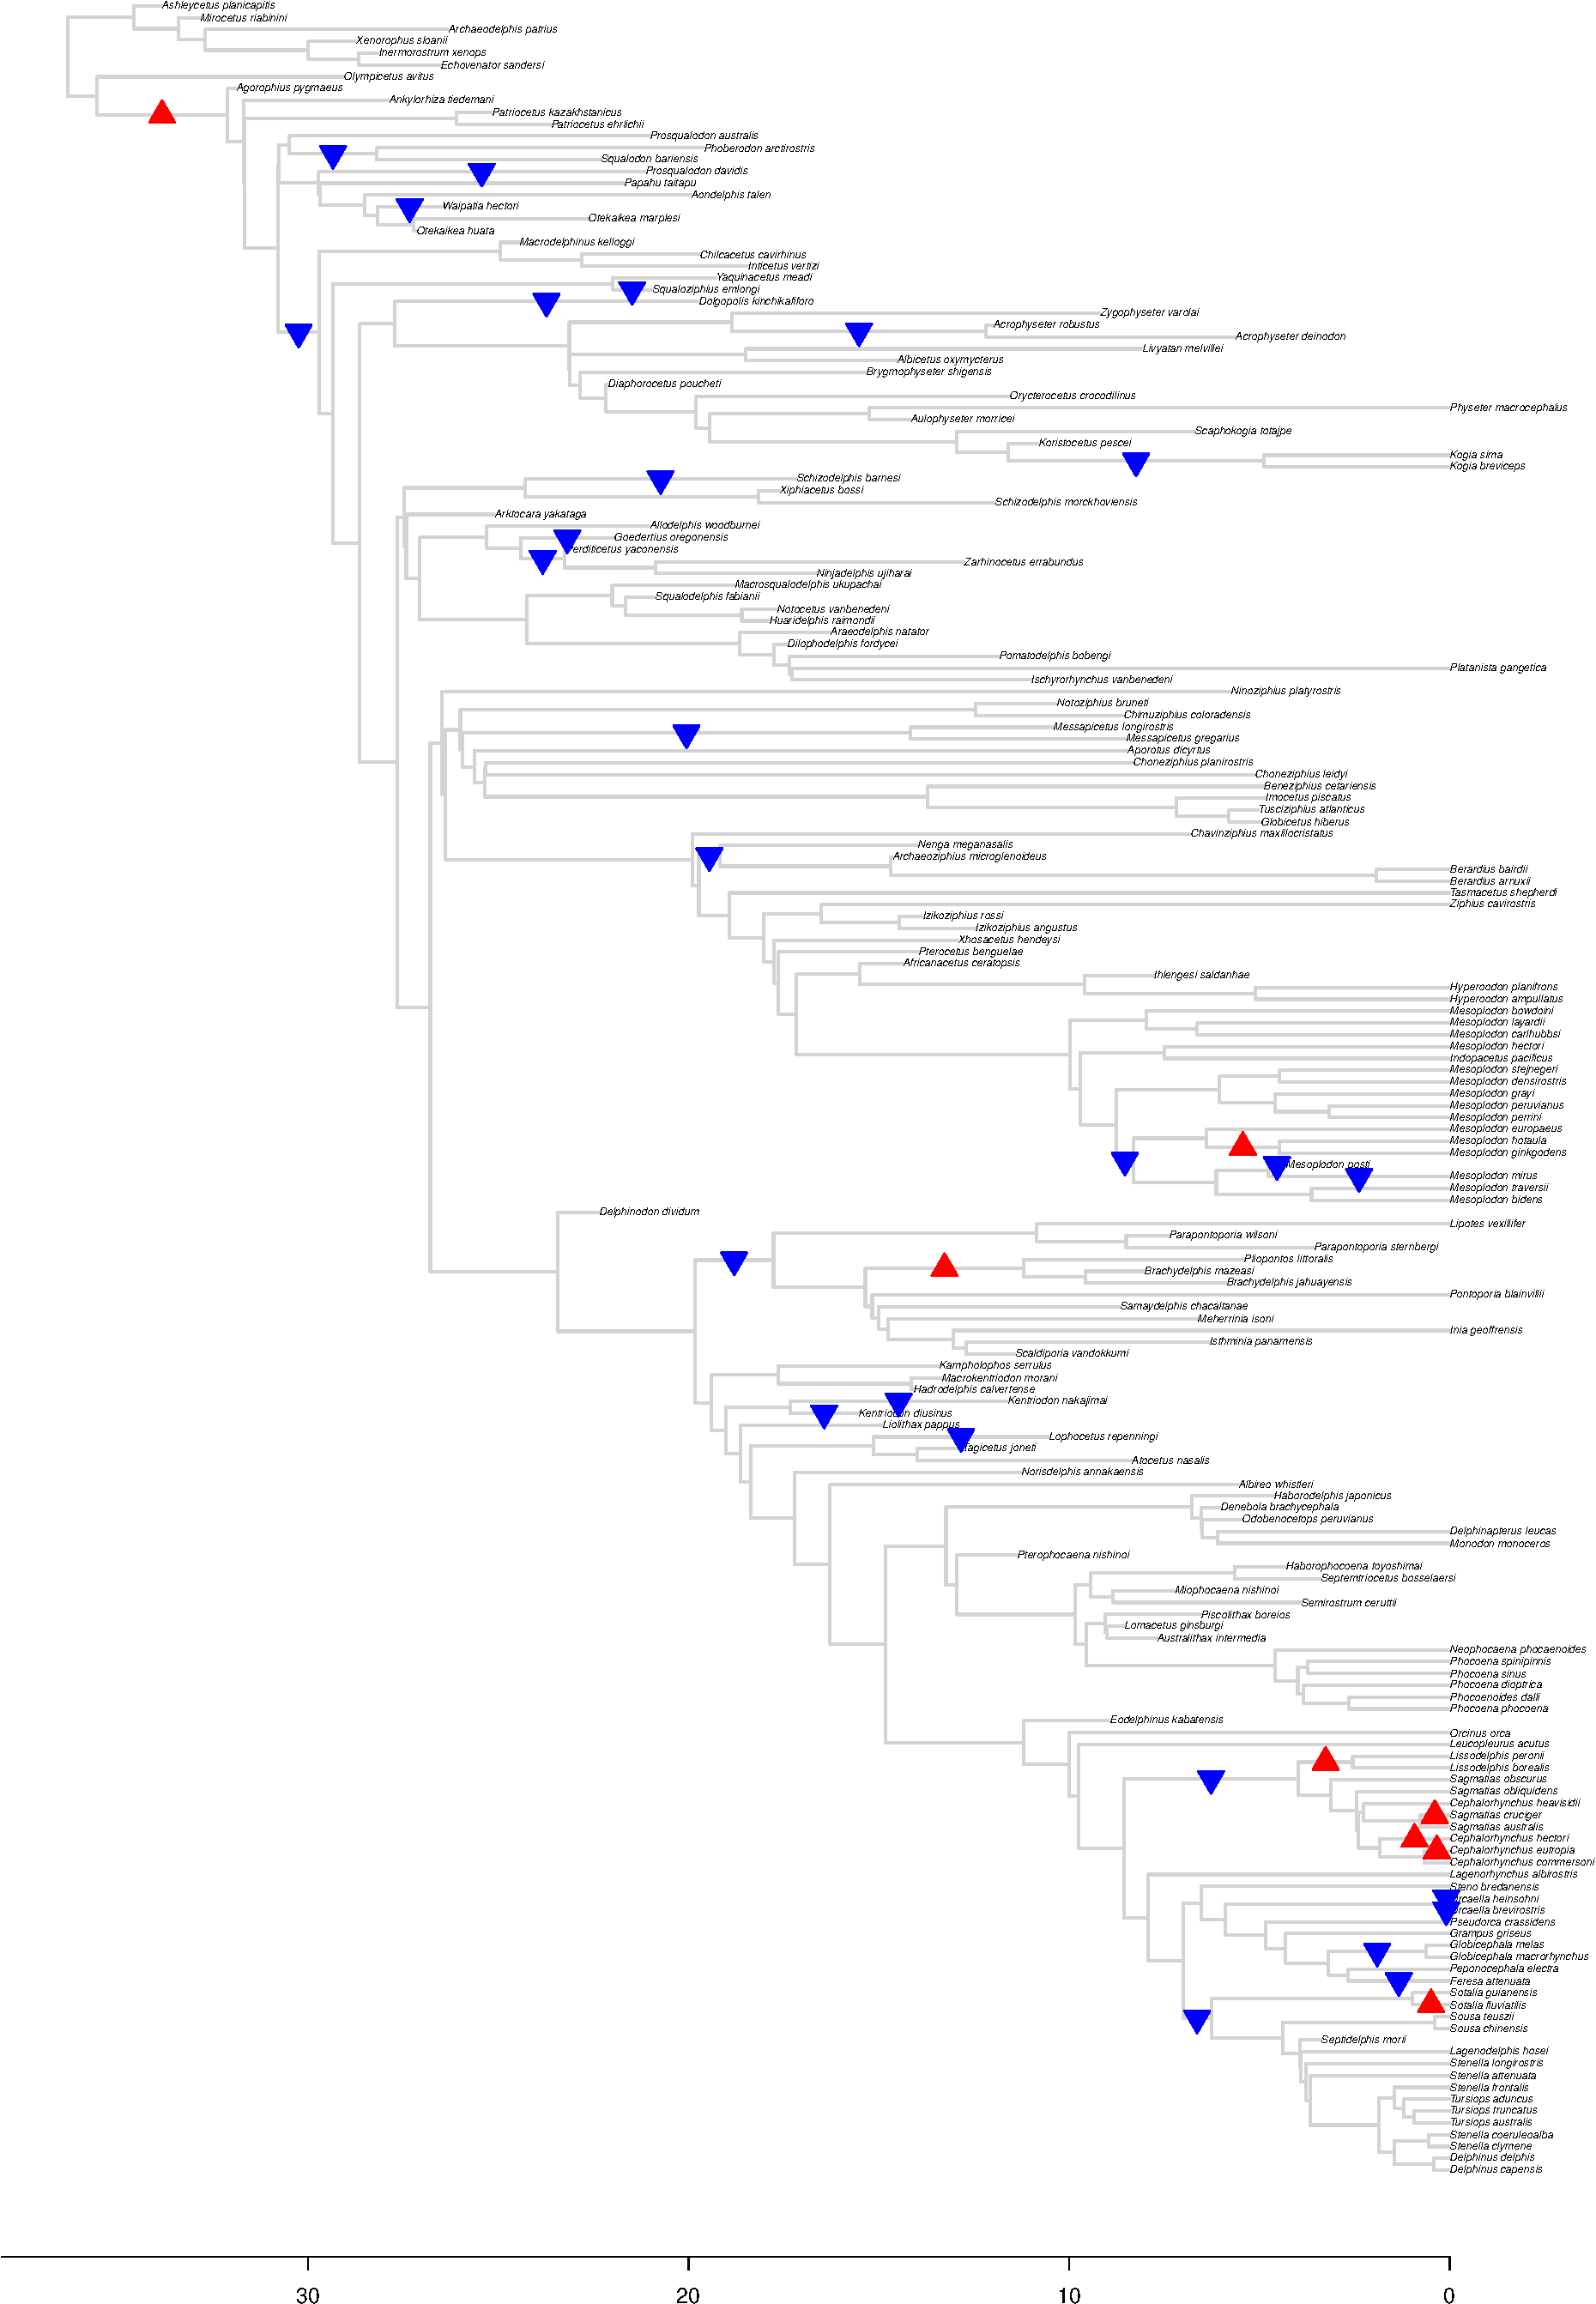
\includegraphics[width=0.9\textwidth]{img/plots-toothed-k15-1.pdf}
\caption{Results for \textit{bayou} fit for the \textit{Toothed} tree, excluding taxa on zero-length branches, setting the average number of shifts in the prior distribution ($\lambda$) to 15. The triangles represent the position and direction of the shifts with posterior probability higher than 0.1, with upward triangles (in red) indicating increases in $\theta$, and downward triangles (in blue) indicating decreases in $\theta$.}
\label{fig:toothed-k15-nzlb}
\end{figure}

\newpage

\begin{figure}[H]
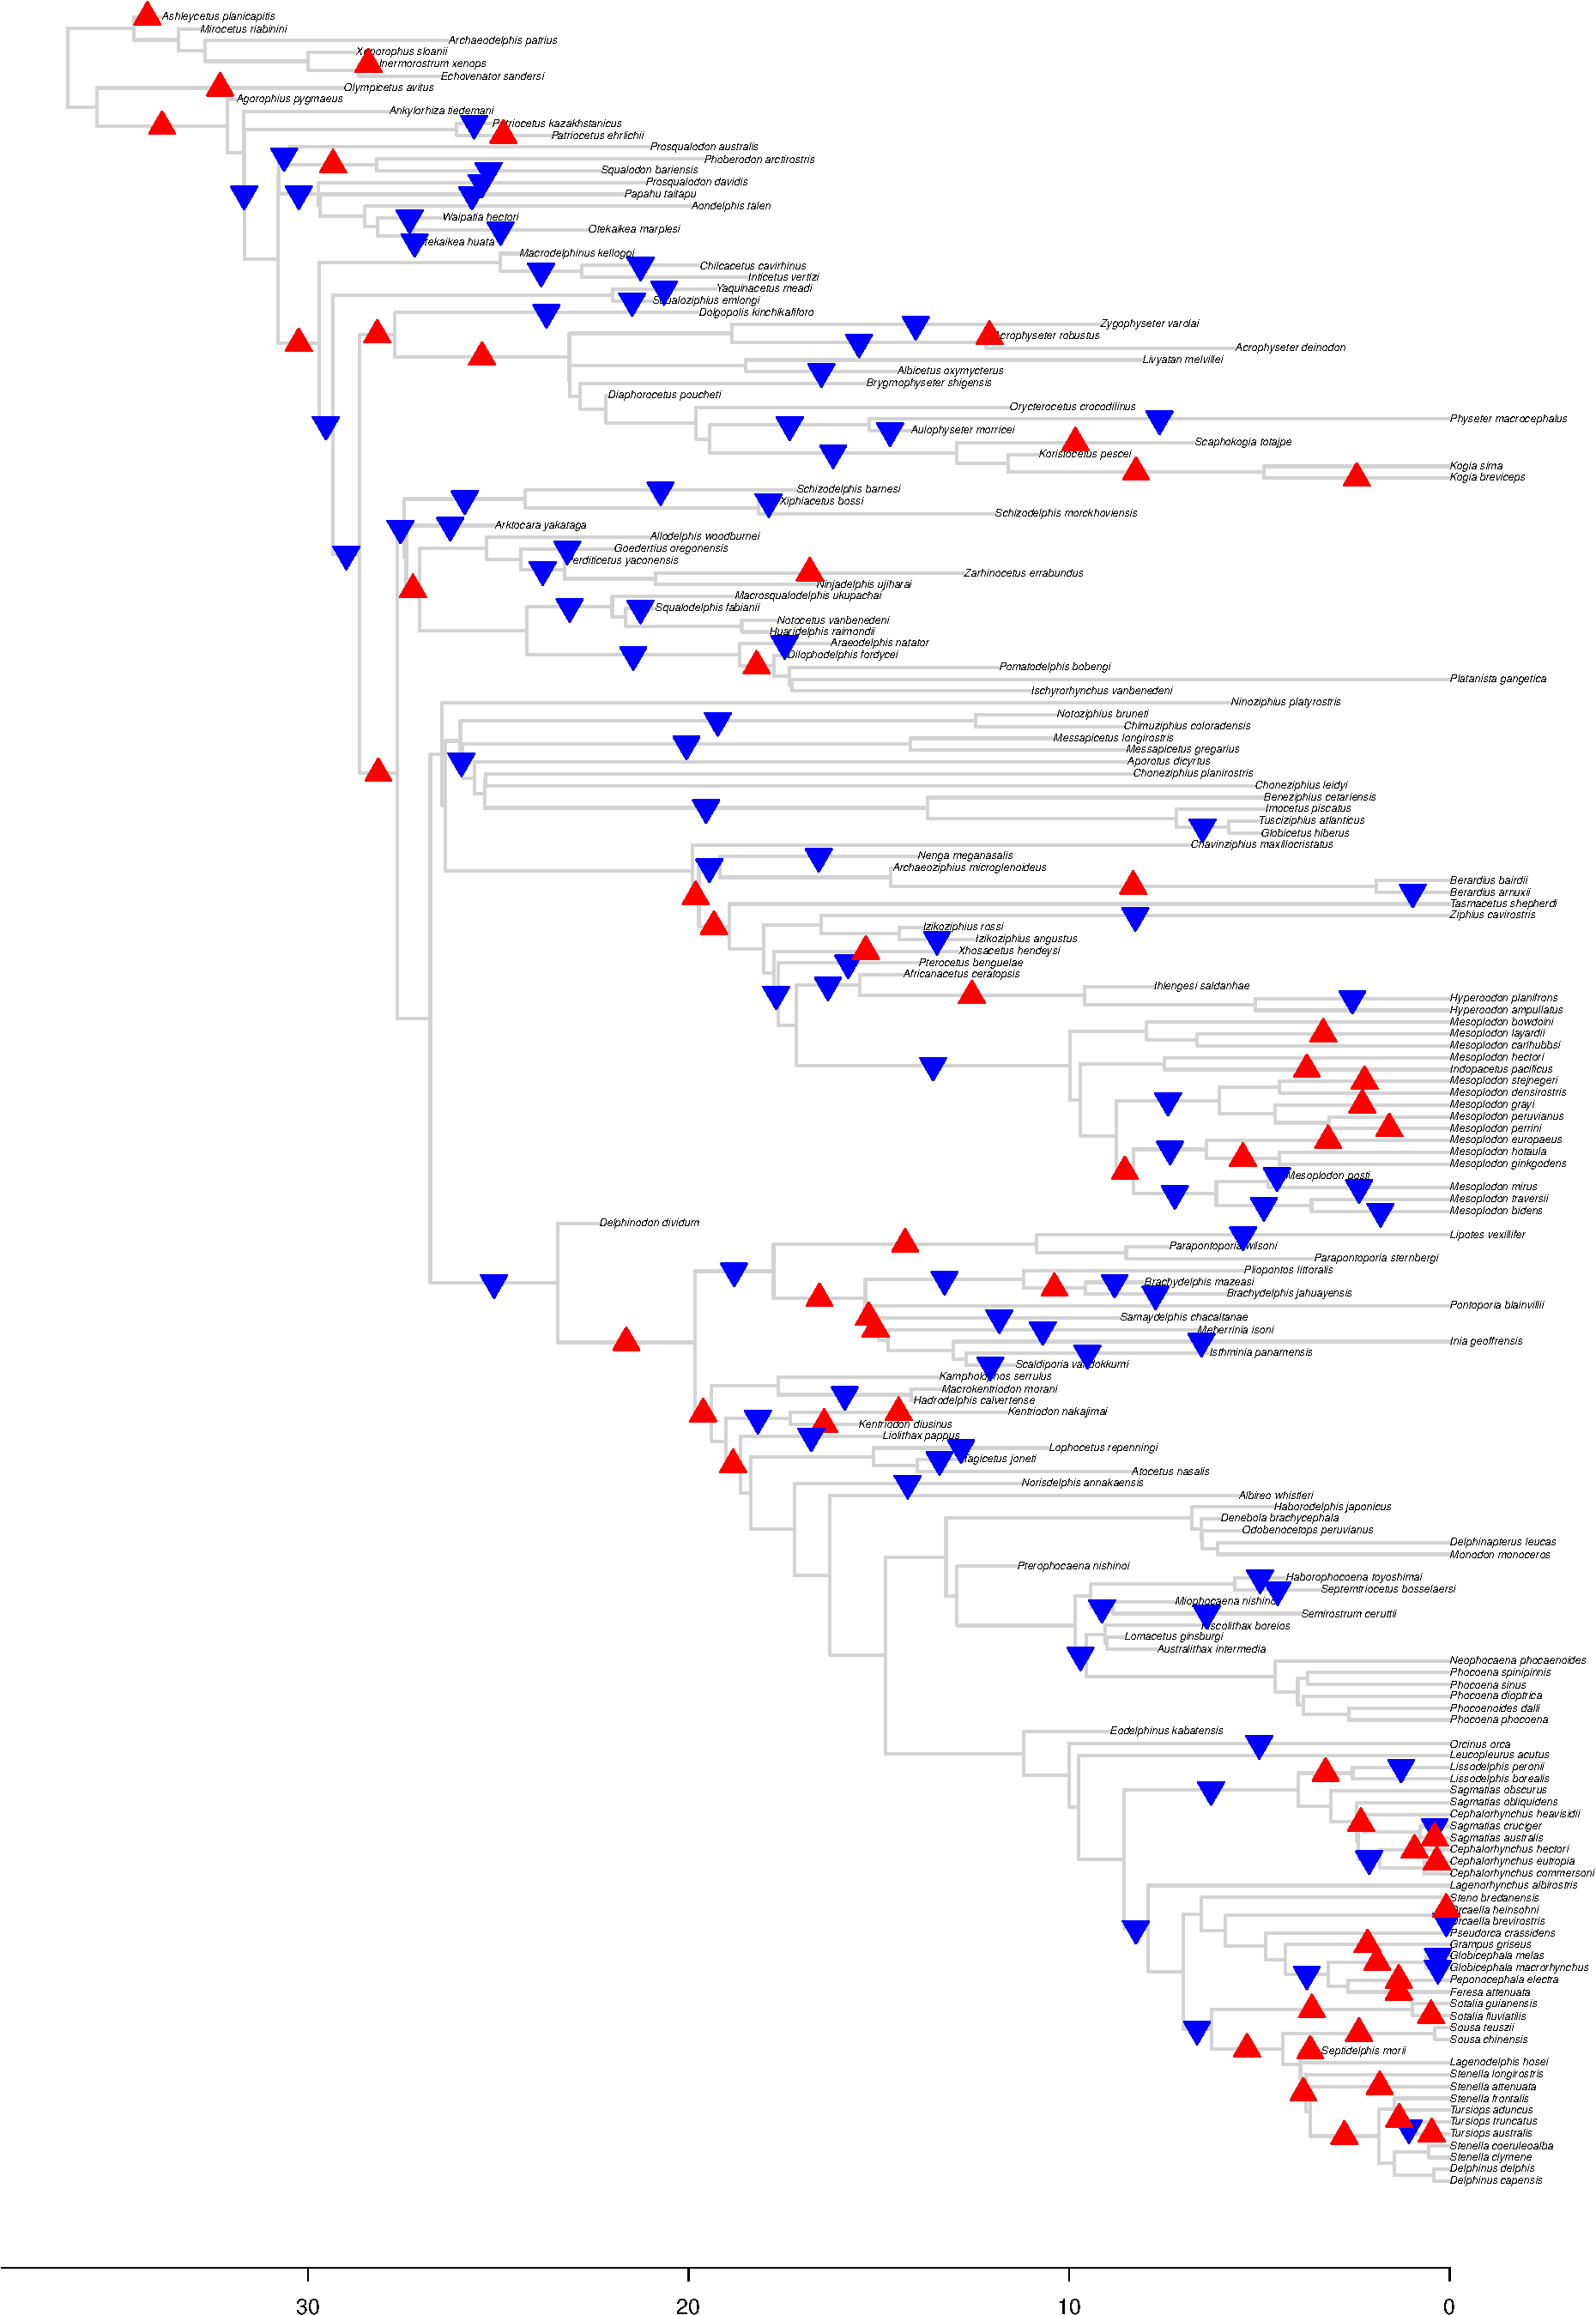
\includegraphics[width=0.9\textwidth]{img/plots-toothed-k50-1.pdf}
\caption{Results for \textit{bayou} fit for the \textit{Toothed} tree, excluding taxa on zero-length branches, setting the average number of shifts in the prior distribution ($\lambda$) to 50. The triangles represent the position and direction of the shifts with posterior probability higher than 0.1, with upward triangles (in red) indicating increases in $\theta$, and downward triangles (in blue) indicating decreases in $\theta$.}
\label{fig:toothed-k50-nzlb}
\end{figure}

\clearpage
